\chapter{\IFRU{Паттерны компиляторов}{Compiler's patterns}}

\IFRU
{Когда я учил Си, а затем Си++, я просто писал небольшие фрагменты кода, компилировал и смотрел что 
получилось на ассемблере. Так намного проще было понять. Я делал это такое количество раз, 
что связь между кодом на \CCpp и тем что генерирует компилятор вбилась мне в подсознание достаточно 
глубоко, поэтому я могу глядя на код на ассемблере сразу понимать, в общих чертах, что там было написано 
на Си. Возможно это поможет кому-то еще, попробую описать некоторые примеры.}
{When I first learned C and then C++ I was just writing small pieces of code, compiling it, 
and seeing what 
was produced in assembly language. That was easy for me. I did it many times and the relation 
between \CCpp code and what the compiler produced was imprinted in my mind so deep that 
I can quickly understand what was in C code when I look at produced x86 code. 
Perhaps this technique may be helpful for someone else so I will try to describe some examples here.}

% sections here:

\section{\HelloWorldSectionName}
\label{sec:helloworld}

\IFRU{Начнем с знаменитого примера из книги}
{Let's start with the famous example from the book}
``The C programming Language''\cite{Kernighan:1988:CPL:576122}:

\lstinputlisting{01_helloworld/1_1.c}

\subsection{x86}

\subsubsection{MSVC}

\IFRU{Компилируем в}{Let's compile it in} MSVC 2010:

\begin{lstlisting}
cl 1.cpp /Fa1.asm
\end{lstlisting}

\IFRU
{(Ключ /Fa означает сгенерировать листинг на ассемблере)}
{(/Fa option means generate assembly listing file)}

\begin{lstlisting}[caption=MSVC 2010]
CONST	SEGMENT
$SG3830	DB	'hello, world', 00H
CONST	ENDS
PUBLIC	_main
EXTRN	_printf:PROC
; Function compile flags: /Odtp
_TEXT	SEGMENT
_main	PROC
	push	ebp
	mov	ebp, esp
	push	OFFSET $SG3830
	call	_printf
	add	esp, 4
	xor	eax, eax
	pop	ebp
	ret	0
_main	ENDP
_TEXT	ENDS
\end{lstlisting}

\IFRU{MSVC выдает листинки в Intel-овском синтаксисе.}{MSVC produces assembly listings in Intel-syntax.} 
\IFRU{Разница между Intel-синтаксисом и AT\&T будет рассмотрена немного позже.}
{The difference between Intel-syntax and AT\&T-syntax will be discussed below.}

\IFRU{Компилятор сгенерировал файл \TT{1.obj}, который впоследствии будет слинкован линкером в \TT{1.exe}.} 
{The compiler generated \TT{1.obj} file will be linked into \TT{1.exe}.}

\IFRU{В нашем случае, этот файл состоит из двух сегментов: \TT{CONST} (для данных-констант) и \TT{\_TEXT} (для кода).}
{In our case, the file contain two segments: \TT{CONST} (for data constants) and \TT{\_TEXT} (for code).} 

\index{\CLanguageElements!const}
\IFRU{Строка \TT{``hello, world''} в \CCpp имеет тип \TT{const char*}, однако не имеет имени.}
{The string \TT{``hello, world''} in \CCpp has type \TT{const char*}, however it does not have
its own name.}

\IFRU{Но компилятору нужно как-то с ней работать, так что он дает ей внутреннее имя \TT{\$SG3830}.}
{The compiler needs to work with the string somehow so it defines the internal name \TT{\$SG3830} for it.}

\IFRU{Как видно, строка заканчивается нулевым байтом ~--- это требования стандарта \CCpp для строк.}
{As we can see, the string is terminated by a zero byte which is standard for \CCpp strings.}

\IFRU{В сегменте кода \TT{\_TEXT}, находится пока только одна функция}
{In the code segment, \TT{\_TEXT}, there is only one function so far}: \main.

\IFRU{Функция \main, как и практически все функции, начинается с пролога и заканчивается эпилогом}
{The function \main starts with prologue code and ends with epilogue code (like almost any function)}
\footnote{\IFRU{Об этом смотрите подробнее в разделе о прологе и эпилоге функции}
{Read more about it in section about function prolog and epilog}
~(\ref{sec:prologepilog}).}.

\index{x86!\Instructions!CALL}
\IFRU{Далее следует вызов функции \printf}
{After the function prologue we see the call to the \printf function}: \TT{CALL \_printf}. 

\index{x86!\Instructions!PUSH}
\IFRU
{Перед этим вызовом, адрес строки (или указатель на нее) с нашим приветствием при помощи инструкции \PUSH помещается в стек.}
{Before the call the string address (or a pointer to it) containing our greeting is placed on the stack with the help of the \PUSH instruction.}

\IFRU{После того как функция \printf возвращает управление в функцию \main, адрес строки (или указатель на нее) все еще лежит в стеке.}
{When the \printf function returns flow control to the \main function, string address (or pointer to it) is still in stack.}

\IFRU{Так как он больше не нужен, то \glslink{stack pointer}{указатель стека} (регистр \ESP) корректируется.} 
{Since we do not need it anymore the \gls{stack pointer} (the \ESP register) needs to be corrected.}

\index{x86!\Instructions!ADD}
\TT{ADD ESP, 4} \IFRU{означает прибавить 4 к значению в регистре \ESP.}
{means add 4 to the value in the \ESP register.}

\IFRU
{Почему 4? Так как, это 32-битный код, для передачи адреса нужно аккурат 4 байта. В x64-коде это 8 байт.}
{Why 4? Since it is 32-bit code we need exactly 4 bytes for address passing through the stack. 
It is 8 bytes in x64-code.}

\TT{``ADD ESP, 4''} \IFRU{эквивалентно \TT{``POP регистр''}, но без использования какого-либо регистра\footnote{Флаги
процессора, впрочем, модифицируются}.}
{is effectively equivalent to \TT{``POP register''} but without using any register\footnote{CPU flags, however, are modified}.}

\index{Intel C++}
\index{Oracle RDBMS}
\index{x86!\Instructions!POP}
\IFRU{Некоторые компиляторы, например Intel C++ Compiler, в этой же ситуации, могут вместо 
\ADD сгенерировать \TT{POP ECX} (подобное можно встретить например в коде \oracle{}, им скомпилированном),
что почти то же самое, только портится значение в регистре \ECX.}
{Some compilers (like Intel C++ Compiler) in the same situation may emit \TT{POP ECX} 
instead of \ADD (e.g. such a pattern can be observed in the \oracle{} code as it is compiled by Intel C++ compiler).
This instruction has almost the same effect but the \ECX register contents will be rewritten.}

\IFRU
{Возможно, компилятор применяет \TT{POP ECX} потому что эта инструкция короче (1 байт против 3).}
{The Intel C++ compiler probably uses \TT{POP ECX} since this instruction's opcode is shorter then 
\TT{ADD ESP, x} (1 byte against 3).}

\IFRU{О стеке можно прочитать в соответствующем разделе}
{Read more about the stack in section}~(\ref{sec:stack}).

\index{\CLanguageElements!return}
\IFRU{После вызова \printf, в оригинальном коде на \CCpp указано \TT{return 0} ~--- вернуть $0$ 
в качестве результата функции \main.} 
{After the call to \printf, in the original \CCpp code was \TT{return 0} ~--- 
return $0$ as the result of the \main function.}

\index{x86!\Instructions!XOR}
\IFRU{В сгенерированном коде это обеспечивается инструкцией}
{In the generated code this is implemented by instruction} \TT{XOR EAX, EAX} 

\index{x86!\Instructions!MOV}
\IFRU{\XOR, на самом деле, как легко догадаться, ``исключающее ИЛИ''}
{\XOR is in fact, just ``eXclusive OR''}
\footnote{\url{http://en.wikipedia.org/wiki/Exclusive_or}}
\IFRU{, но компиляторы часто используют его вместо простого}
{but compilers often use it instead of}
\TT{MOV EAX, 0} ~--- 
\IFRU
{снова потому что опкод короче (2 байта против 5).}
{again because it is a slightly shorter opcode (2 bytes against 5).}

\index{x86!\Instructions!SUB}
\IFRU{Бывает так, что некоторые компиляторы генерируют}{Some compilers emit}
\TT{SUB EAX, EAX}, 
\IFRU
{что значит, \IT{отнять значение в \EAX от значения в \EAX}, что в любом случае даст 0 в результате.}
{which means \IT{SUBtract the value in the \EAX from the value in \EAX}, which in any case will result zero.}

\index{x86!\Instructions!RET}
\IFRU{Самая последняя инструкция \RET возвращает управление в вызывающую функцию.
Обычно, это код \CCpp \ac{CRT}, который, в свою очередь, 
вернет управление операционной системе.}
{The last instruction \RET returns control flow to the \gls{caller}.
Usually, it is \CCpp \ac{CRT} code which in turn returns control to the \ac{OS}.}

\subsubsection{GCC}

\IFRU{Теперь скомпилируем то же самое компилятором GCC 4.4.1 в Linux}
{Now let's try to compile the same \CCpp code in the GCC 4.4.1 compiler in Linux}: \TT{gcc 1.c -o 1}

\IFRU{Затем при помощи \IDA. посмотрим как создалась функция \main.}
{After, with the assistance of the \IDA disassembler, let's see how the \main function was created.} 

(\IDA, \IFRU{как и MSVC, показывает код в Intel-синтаксисе}{as MSVC, showing code in Intel-syntax}).

N.B. \IFRU{Мы также можем заставить GCC генерировать листинги в этом формате при помощи ключей}
{We could also have GCC produce assembly listings in Intel-syntax by applying the options} 
\TT{-S -masm=intel}

\begin{lstlisting}[caption=GCC]
main            proc near

var_10          = dword ptr -10h

                push    ebp
                mov     ebp, esp
                and     esp, 0FFFFFFF0h
                sub     esp, 10h
                mov     eax, offset aHelloWorld ; "hello, world"
                mov     [esp+10h+var_10], eax
                call    _printf
                mov     eax, 0
                leave
                retn
main            endp
\end{lstlisting}

\index{Function prologue}
\index{x86!\Instructions!AND}
\IFRU{Почти то же самое. 
Адрес строки ``hello, world'' лежащей в сегменте данных, в начале сохраняется в \EAX, затем записывается в стек.
А еще в прологе функции мы видим \TT{AND ESP, 0FFFFFFF0h} ~--- 
эта инструкция выравнивает значение в \ESP по 16-байтной границе, делая все значения 
в стеке также выровненными по этой границе (процессор более эффективно работает с переменными расположенными
в памяти по адресам кратным 4 или 16)\footnote{\URLWPDA}.}
{The result is almost the same.
The address of the ``hello world'' string (stored in the data segment) is saved in the \EAX register first then it is stored on the stack.
Also in the function prologue we see \TT{AND ESP, 0FFFFFFF0h} ~--- 
this instruction aligns the value in the \ESP register on a 16-byte border.
This results in all values in the stack being aligned.
(CPU performs better if the values it is working with are located in memory at addresses aligned 
on a 4 or 16 byte border)\footnote{\URLWPDA}.}

\index{x86!\Instructions!SUB}
\TT{SUB ESP, 10h} \IFRU{выделяет в стеке 16 байт. Хотя, как будет видно далее, здесь достаточно только 4.}
{allocates 16 bytes on the stack. Although, as we can see below, only 4 are necessary here.} 

\IFRU{Это происходит потому что количество выделяемого места в локальном стеке тоже выровнено по 
16-байтной границе.}
{This is because the size of the allocated stack is also aligned on a 16-byte border.}

% TODO: rewrite.
\index{x86!\Instructions!PUSH}
\IFRU{Адрес строки (или указатель на строку) затем записывается прямо в стек без помощи инструкции \PUSH.
\IT{var\_10} по совместительству ~--- и локальная переменная и одновременно аргумент для \printf{}. Подробнее об этом будет ниже.}
{The string address (or a pointer to the string) is then written directly on the stack space 
without using the \PUSH instruction.
\IT{var\_10} ~--- is a local variable but is also an argument for \printf{}.
Read about it below.}

\IFRU{Затем вызывается \printf.}{Then the \printf function is called.}

\IFRU{В отличие от MSVC, GCC в компиляции без включенной оптимизации генерирует \TT{MOV EAX, 0} вместо 
более короткого опкода.}{Unlike MSVC, when GCC is compiling without optimization turned on,
it emits \TT{MOV EAX, 0} instead of a shorter opcode.}

\index{x86!\Instructions!LEAVE}
\IFRU{Последняя инструкция \LEAVE ~--- это аналог команд \TT{MOV ESP, EBP} и \TT{POP EBP} ~--- 
то есть возврат \glslink{stack pointer}{указателя стека} и регистра \EBP в первоначальное состояние.} 
{The last instruction, \LEAVE ~--- is the equivalent of the \TT{MOV ESP, EBP} and \TT{POP EBP} instruction pair ~--- 
in other words, this instruction sets the \gls{stack pointer} (\ESP) back and restores 
the \EBP register to its initial state.}

\IFRU{Это необходимо, т.к., в начале функции мы модифицировали регистры \ESP и \EBP (при помощи}
{This is necessary since we modified these register values (\ESP and \EBP) at the 
beginning of the function (executing}
\TT{\MOV EBP, ESP} / \TT{AND ESP, ...}).

\subsubsection{GCC: \ATTSyntax}

\IFRU{Попробуем посмотреть, как выглядит то же самое в AT\&T-синтаксисе языка ассемблера.}
{Let's see how this can be represented in the AT\&T syntax of assembly language.}
\IFRU{Этот синтаксис больше распространен в UNIX-мире.}
{This syntax is much more popular in the UNIX-world.}

\begin{lstlisting}[caption=\IFRU{компилируем в}{let's compile in} GCC 4.7.3]
gcc -S 1_1.c
\end{lstlisting}

\IFRU{Получим такой файл:}{We get this:}

\lstinputlisting[caption=GCC 4.7.3]{01_helloworld/1_1.s}

\IFRU{Здесь много макросов (начинающихся с точки). Они нам пока не интересны.}
{There are a lot of macros (beginning with dot). These are not very interesting to us so far.}
\IFRU{Пока что, ради упрощения, мы можем
их игнорировать и впредь (кроме макроса \IT{.string}, при помощи которого кодируется последовательность символов 
оканчивающихся нулем, такие же строки как в Си). И тогда получится следующее}
{For now, for the sake of simplification, we can ignore them (except the \IT{.string} macro which
encodes a null-terminated character sequence just like a C-string). Then we'll see this}
\footnote{\IFRU{Кстати, для уменьшения генерации ``лишних'' макросов, можно использовать такой ключ GCC}
{This GCC option can be used to eliminate ``unnecessary'' macros}: 
\IT{-fno-asynchronous-unwind-tables}}:

\lstinputlisting[caption=GCC 4.7.3]{01_helloworld/1_1_refined.s}

\index{\ATTSyntax}
\index{\IntelSyntax}
\IFRU{Основные отличия синтаксиса Intel и AT\&T следующие:}
{Some of the major differences between Intel and AT\&T syntax are:}

\begin{itemize}

\item
\IFRU{Операнды записываются наоборот.}{Operands are written backwards.}

\IFRU{В Intel-синтаксисе: <инструкция> <операнд назначения> <операнд-источник>.}
{In Intel-syntax: <instruction> <destination operand> <source operand>.}

\IFRU{В AT\&T-синтаксисе: <инструкция> <операнд-источник> <операнд назначения>.}
{In AT\&T syntax: <instruction> <source operand> <destination operand>.}

\IFRU{Чтобы легче понимать разницу, можно запомнить следующее}
{Here is a way to think about them}: \IFRU{когда вы работаете с Intel-синтаксисом, можете в уме ставить знак равенства ($=$) между операндами,}
{when you work with Intel-syntax, you can put in equality sign ($=$) in your mind between operands}
\IFRU{а когда с AT\&T-синтаксисом, мысленно ставьте стрелку направо}
{and when you work with AT\&T-syntax put in a right arrow} 
($\rightarrow$)
\footnote{
\index{\CStandardLibrary!memcpy()}
\index{\CStandardLibrary!strcpy()}
\IFRU{Кстати, в некоторые стандартных функциях библиотеки Си (например, memcpy(), strcpy()) также применяется 
расстановка аргументов как в Intel-синтаксисе: в начале указатель в памяти на блок назначения, 
затем указатель на блок-источник.}{By the way, in some C standard functions (e.g., memcpy(), strcpy()) arguments
are listed in the same way as in Intel-syntax: pointer to destination memory block at the beginning and then
pointer to source memory block.}}.

\item
AT\&T: \IFRU{Перед именами регистров ставится знак процента (\%), а перед числами знак доллара (\$).}
{Before register names a percent sign must be written (\%) and before numbers a dollar sign (\$).}
\IFRU{Вместо квадратных скобок применяются круглые.}{Parentheses are used instead of brackets.}

\item
AT\&T: \IFRU{К каждой инструкции добавляется специальный символ, определяющий тип данных:}
{A special symbol is to be added to each instruction defining the type of data:}

\begin{itemize}
\item l --- long (32 \IFRU{бита}{bits})
\item w --- word (16 \IFRU{бит}{bits})
\item b --- byte (8 \IFRU{бит}{bits})
\end{itemize}

\end{itemize}

\IFRU{Возвращаясь к результату компиляции: он идентичен тому, который мы посмотрели в \IDA.}
{Let's go back to the compilation result: it is identical to which we saw in \IDA.}
\IFRU{Одна мелочь}{With one subtle difference}: \TT{0FFFFFFF0h} \IFRU{записывается как}{is written as} \TT{\$-16}.
\IFRU{Это тоже самое}{It is the same}: \TT{16} \IFRU{в десятичной системе это}{in the decimal system is} \TT{0x10} 
\IFRU{в шестнадцатеричной}{in hexadecimal}. 
\TT{-0x10} \IFRU{будет как раз}{is equal to} \TT{0xFFFFFFF0} 
(\IFRU{в рамках 32-битных чисел}{for a 32-bit data type}).




\subsection{ARM}
\label{sec:hw_ARM}

\index{\idevices}
\index{Raspberry Pi}
\index{Xcode}
\index{LLVM}
\index{Keil}
\IFRU{Для экспериментов с процессором ARM, я выбрал два компилятора}
{For my experiments with ARM processors I chose two compilers}: 
\IFRU{популярный в embedded-среде}{popular in the embedded area} Keil Release 6/2013 
\IFRU{и среду разработки}{and} Apple Xcode 4.6.3 \IFRU{}{IDE} (\IFRU{с компилятором}{with} LLVM-GCC 4.2 \IFRU{}{compiler}), 
\IFRU{генерирующую код для ARM-совместимых процессоров и}{which produces code for ARM-compatible processors and} \ac{SOC} \InENRU \idevices, 
\IFRU{планшетных компьютеров для Windows 8 и Windows RT}{Windows 8 and Window RT tables}\footnote{\url{http://en.wikipedia.org/wiki/List_of_Windows_8_and_RT_tablet_devices}} 
\IFRU{и таких устройствах как}{and also such devices as} Raspberry Pi.

\subsubsection{\NonOptimizingKeil + \ARMMode}

\IFRU{Для начала, скомпилируем наш пример в Keil}{Let's start by compiling our example in Keil}:

\begin{lstlisting}
armcc.exe --arm --c90 -O0 1.c 
\end{lstlisting}

\index{\IntelSyntax}
\IFRU{Компилятор \IT{armcc} генерирует листинг на ассемблере в формате Intel,}
{The \IT{armcc} compiler produces assembly listings in Intel-syntax} 
\IFRU{но он содержит некоторые высокоуровневые макросы связанные с ARM}
{but it has a high-level ARM-processor related macros}\footnote{
\IFRU{например, он показывает инструкции \PUSH/\POP отсутствующие в режиме ARM}
{e.g. ARM mode lacks \PUSH/\POP instructions}}, 
\IFRU{а нам важнее увидеть инструкции ``как есть'', так что посмотрим скомпилированный результат в \IDA}
{but it is more important for us to see instructions ``as is'' so let's see the compiled results in \IDA}.

\begin{lstlisting}[caption=\NonOptimizingKeil + \ARMMode + \IDA]
.text:00000000             main
.text:00000000 10 40 2D E9                 STMFD   SP!, {R4,LR}
.text:00000004 1E 0E 8F E2                 ADR     R0, aHelloWorld ; "hello, world"
.text:00000008 15 19 00 EB                 BL      __2printf
.text:0000000C 00 00 A0 E3                 MOV     R0, #0
.text:00000010 10 80 BD E8                 LDMFD   SP!, {R4,PC}

.text:000001EC 68 65 6C 6C+aHelloWorld     DCB "hello, world",0    ; DATA XREF: main+4
\end{lstlisting}

\index{ARM!\ARMMode}
\index{ARM!\ThumbMode}
\index{ARM!\ThumbTwoMode}
\IFRU{Вот чуть-чуть фактов о процессоре ARM, которые желательно знать}
{Here are a couple of ARM-related facts we should know in order to proceed}.
\IFRU{Процессор ARM имеет по крайней мере два основных режима: режим ARM и thumb}
{An ARM processor has at least two major modes: ARM mode and thumb}. 
\IFRU{В первом (ARM) режиме доступны все инструкции и каждая имеет размер 32 бита (или 4 байта)}
{In the first (ARM) mode all instructions are enabled and each has 32-bit (4 bytes) size}. 
\IFRU{Во втором режиме (thumb) каждая инструкция имеет размер 16 бит (или 2 байта)}
{In the second (thumb) mode each instruction has 16-bit (or 2 bytes) size}
\footnote{\IFRU{Кстати, инструкции фиксированного размера удобны тем, что всегда можно легко узнать адрес 
следующей (или предыдущей) инструкции. Эта особенность будет рассмотрена в секции о 
switch()~(\ref{sec:SwitchARMLot}).}
{By the way, fixed-length instructions are handy in a way that one can calculate the next (or previous) 
instruction's address without effort. This feature will be discussed in switch()~(\ref{sec:SwitchARMLot}) section.}
}.
\IFRU{Режим thumb может выглядеть привлекательнее тем, что программа на нем может быть 1) компактнее; 2) эффективнее исполняться на микроконтроллере с 16-битной шиной данных}
{Thumb mode may look attractive because programs that use it may 1) be compact and
2) execute faster on microcontrollers having a 16-bit memory datapath}. 
\IFRU{Но за всё нужно платить: в режиме thumb куда меньше возможностей процессора, например, возможен доступ только к 8-и регистрам процессора, и чтобы совершить некоторые действия, выполнимые в режиме ARM одной инструкцией, нужны несколько thumb-инструкций}
{Nothing comes free of charge, so, in thumb mode there is a reduced instruction set, 
only 8 registers are accessible and one needs several thumb instructions for doing some operations when in ARM mode you only need one}.
\IFRU{Начиная с ARMv7, имеется также поддержка инструкций thumb-2, это thumb расширенный до поддержки куда большего числа инструкций}
{Starting at ARMv7 the thumb-2 instruction set is also present. 
This is an extended thumb which supports a much larger instruction set}.
\IFRU{Распространено заблуждение что thumb-2 это смесь ARM и thumb. Это не верно. Просто thumb-2 был дополен до
более полной поддержки возможностей процессора, что теперь может легко конкурировать с режимом ARM.}
{There is a common misconception the thumb-2 is a mix of ARM and thumb. This is not correct. 
Rather, thumb-2 was extended to fully support processor features so it could
compete with ARM mode.}
\IFRU{Программа для процессора ARM может представлять смесь процедур скомпилированных для обоих режимов}
{A program for ARM processor may be a mix of procedures compiled for both modes}.
\IFRU{Основное количество приложений для \idevices скомпилировано для набора инструкций thumb-2, потому что Xcode
делает так по умолчанию}
{The majority of \idevices applications are compiled for thumb-2 instructions set because Xcode does this by default}.

\IFRU{В вышеприведененном примере можно легко увидеть что каждая инструкция имеет размер 4 байта}
{In the example we can easily see each instruction has a size of 4 bytes}.
\IFRU{Действительно, ведь мы же компилировали наш код для режима ARM а не thumb}
{Indeed, we compiled our code for ARM mode, not for thumb}.

\index{ARM!\Instructions!STMFD}
\index{ARM!\Instructions!POP}
\IFRU{Самая первая инструкция}{The very first instruction}, \TT{''STMFD SP!, \{R4,LR\}''}\footnote{\STMFDdesc}, 
\IFRU{работает как инструкция}{works as an x86} \PUSH \IFRU{в x86}{instruction},
\IFRU{записывает значения двух регистров}{writing the values of two registers}
(\Rfour \AndENRU \LR) \IFRU{в стек}{into the stack}.
\IFRU{Действительно, в выдаваемом листинге на ассемблере, компилятор \IT{armcc}, для упрощения, указывает здесь инструкцию}
{Indeed, in the output listing from the \IT{armcc} compiler, for the sake of simplification, 
actually shows the} \TT{''PUSH \{r4,lr\}''}\IFRU{}{ instruction}.
\IFRU{Но это не совсем точно, инструкция \PUSH доступна только в режиме thumb, поэтому,
во избежания путанницы, я предложил работать в \IDA}
{But it is not quite correct. \PUSH instruction are only available in thumb mode.
So, to make things less messy, I offered to work in \IDA}.

\IFRU{Итак, эта инструкция записывает значения регистров \Rfour и \LR по адресу в памяти, на который указывает регистр \SPwithfootnote, затем уменьшает \TT{SP}, 
чтобы он указывал на место в стеке, доступное для новых записей}
{This instruction writes the values of the \Rfour and \LR registers at the address in memory to which 
\SPwithfootnote is pointing, then it \glspl{decrement} \SP so it will point to the place in the stack that 
is free for new entries}.

\IFRU{Эта инструкция, как и инструкция \PUSH в режиме thumb, может сохранить в стеке одновременно несколько значений регистров, что может быть очень удобно}
{This instruction (like the \PUSH instruction in thumb mode) is able to save several register values at once and this may be useful}. 
\IFRU{Кстати, такого в x86 нет}{By the way, there is no such thing in x86}.
\IFRU{Так же следует заметить, что \TT{STMFD} ~--- генерализация инструкции \PUSH (то есть, расширяет её возможности), потому что может работать с любым регистром а не только с \SP, это тоже может быть очень удобно}
{It can also be noted the \TT{STMFD} instruction is a generalization 
of \PUSH instruction (extending its features), since it can work with any register, not just with \SP and this can be very useful}.

\index{\PICcode}
\index{ARM!\Instructions!ADR}
\IFRU{Инструкция}{The} \TT{''ADR R0, aHelloWorld''}
\IFRU{прибавляет значение регистра \PC к смещению, где хранится строка}
{instruction adds the value in the \PC register to the offset where the}
\IT{``hello, world''} \IFRU{}{string is located}.
\IFRU{Причем здесь \PC, можно спросить}{How \TT{PC} register used here, one might ask}?
\IFRU{Притом, что это так называемый ``\PICcode''}{This is so called ``\PICcode''.}
\footnote{
	\IFRU{Читайте больше об этом в соответствующем разделе}
	{Read more about it in relevant section}~(\ref{sec:PIC})
	},
\IFRU{он предназначен для исполнения будучи не привязанным к каким-либо адресам в памяти}
{It is intended to be executed at an unfixed addresses in memory}.
\IFRU{В опкоде инструкции \TT{ADR} указывается разница между адресом этой инструкции и местом, где хранится строка}
{In the opcode of the \TT{ADR} instruction is encoded the difference between the address of this instruction and the place where the string is located}.
\IFRU{Эта разница всегда будет постоянной, вне зависимости от того, куда был загружен \ac{OS}
наш код}
{The difference will always be the same,
independent from the address where the code is loaded by \ac{OS}}.
\IFRU{Поэтому всё что нужно это прибавить адрес текущей инструкции (из \PC) чтобы получить текущий абсолютный адрес нашей Си-строки}
{That's why all we need is to add the address of the current instruction (from \PC) in order to get the absolute address of our C-string in memory}.

\index{ARM!\Registers!Link Register}
\index{ARM!\Instructions!BL}
\IFRU{Инструкция}{} \TT{''BL \_\_2printf''}\footnote{Branch with Link}
\IFRU{вызывает функцию \printf}{instruction calls the \printf function}. 
\IFRU{Работа этой инструкции состоит из двух фаз}
{That's how this instruction works}: 
\begin{itemize}
\item
\IFRU{записать адрес после инструкции \TT{BL} (\TT{0xC}) в регистр \LR}
{write the address following the \TT{BL} instruction (\TT{0xC}) into the \LR};
\item
\IFRU{затем собственно передать управление в \printf, записав адрес этой функции в регистр \PCwithfootnote}
{then pass control flow into \printf by writing its address into the \PCwithfootnote register}.
\end{itemize}

\IFRU{Ведь, когда функция \printf закончит работу, нужно знать, куда вернуть управление, поэтому закончив работу, всякая функция передает управление по адресу записанному в регистре \LR}
{When \printf finishes its work it must have information about where it must return control.
That's why each function passes control to the address stored in the \LR register}.

\IFRU{В этом разница между ``чистыми'' \ac{RISC}-процессорами вроде ARM и \ac{CISC}-процессорами как x86,
где адрес возврата записывается в стек}
{That is the difference between ``pure'' \ac{RISC}-processors like ARM and \ac{CISC}-processors like x86,
where address of return is stored in stack}\footnote{\IFRU{Подробнее об этом будет описано в следующей главе}{Read more about this in next section}~(\ref{sec:stack})}.

\IFRU{Кстати, 32-битный абсолютный адрес, либо же смещение, невозможно закодировать в 32-битной инструкции \TT{BL}, в ней есть место только для 24-х бит}
{By the way, an absolute 32-bit address or offset cannot be encoded in the 32-bit \TT{BL} instruction because
it only has space for 24 bits}.
\IFRU{Так же следует отметить, что из-за того что все инструкции в режиме ARM имеют длину 4 байта (32 бита), и инструкции могут находится только по адресам кратным 4, то последние 2 бита (всегда нулевых) можно не кодировать.}
{It is also worth noting all ARM mode instructions have a size of 4 bytes (32 bits).
Hence they can only be located on 4-byte boundary addresses.
This means the the last 2 bits of the instruction address (always zero bits) may be omitted.}
\IFRU{В итоге имеем 26 бит, при помощи которых можно закодировать смещение}
{In summary, we have 26 bit for offset encoding. This is enough to represent offset} $\pm{}\approx{}32M$.

\index{ARM!\Instructions!MOV}
\IFRU{Следующая инструкция}{Next, the} \TT{''MOV R0, \#0''}\footnote{MOVe}
\IFRU{просто записывает $0$ в регистр \Rzero}{instruction just writes $0$ into the \Rzero register}.
\IFRU{Ведь наша Си-функция возвращает $0$ а возвращаемое значение всякая функция оставляет в \Rzero}
{That's because our C-function returns $0$ and the returned value is to be placed in the \Rzero register}.

\index{ARM!\Registers!Link Register}
\index{ARM!\Instructions!LDMFD}
\index{ARM!\Instructions!POP}
\IFRU{Последняя инструкция}{The last instruction} \TT{''LDMFD SP!, {R4,PC}''}\footnote{\LDMFDDESC} \IFRU{это инструкция обратная от}{is an inverse instruction of} \TT{STMFD}. 
\IFRU{Она загружает из стека значения для сохранения их в \Rfour и \PC, увеличивая \glslink{stack pointer}{указатель стека} \SP}
{It loads values from the stack in order to save them into \Rfour and \PC, and \glslink{increment}{increments} \gls{stack pointer} \SP}.
\IFRU{Это, в каком-то смысле, аналог \POP}{It can be said it is similar to \POP}. 
N.B. \IFRU{Самая первая инструкция \TT{STMFD} сохранила в стеке \Rfour и \LR, а \IT{восстанавливаются} во время исполнения \TT{LDMFD} регистры \Rfour и \PC}
{The very first instruction \TT{STMFD} saves the \Rfour and \LR registers pair on the stack, but \Rfour and \PC are \IT{restored} during execution of \TT{LDMFD}}.
\IFRU{Как я уже описывал, в регистре \LR обычно сохраняется адрес места, куда нужно всякой функции вернуть управление}
{As I wrote before, address of place to where each function must return control is usually saved in the \LR
register}.
\IFRU{Самая первая инструкция сохраняет это значение в стеке, потому что наша функция \main позже будет сама пользоваться этим регистром, в момент вызова \printf}
{The very first function saves its value in the stack because our
\main function will use the register in order to call \printf}.
\IFRU{А затем, в конце функции, это значение можно сразу записать в \PC, таким образом, передав управление туда, откуда была вызвана наша функция}
{In the function end this value can be written to the \PC register, thus passing control to where our function was called}.
\IFRU{Так как функция \main обычно самая главная в \CCpp, управление будет возвращено в загрузчик \ac{OS}, либо куда-то в \ac{CRT},
или что-то в этом роде}
{Since our \main function is usually the primary function in \CCpp,
control will be returned to \ac{OS} loader or to a point in \ac{CRT},
or something like that}.

\index{ARM!DCB}
\TT{DCB}\IFRU{ ~--- директива ассемблера, описывающая массивы байт или ASCII-строк, аналог директивы DB в 
x86-ассемблере}
{~---assembly language directive defining array of bytes or ASCII-strings, akin to the DB directive 
in x86-assembly language}.

\subsubsection{\NonOptimizingKeil: \ThumbMode}

\IFRU{Скомпилируем тот же пример в Keil для режима thumb}{Let's compile the same example using Keil in thumb mode}:

\begin{lstlisting}
armcc.exe --thumb --c90 -O0 1.c 
\end{lstlisting}

\IFRU{Получим (в \IDA)}{We will get (in \IDA)}:

\begin{lstlisting}[caption=\NonOptimizingKeil + \ThumbMode + \IDA]
.text:00000000             main
.text:00000000 10 B5                       PUSH    {R4,LR}
.text:00000002 C0 A0                       ADR     R0, aHelloWorld ; "hello, world"
.text:00000004 06 F0 2E F9                 BL      __2printf
.text:00000008 00 20                       MOVS    R0, #0
.text:0000000A 10 BD                       POP     {R4,PC}

.text:00000304 68 65 6C 6C+aHelloWorld     DCB "hello, world",0    ; DATA XREF: main+2
\end{lstlisting}

\IFRU{Сразу бросаются в глаза двухбайтные (16-битные) опкоды, это, как я уже упоминал, thumb}
{We can easily spot the 2-byte (16-bit) opcodes. This is, as I mentioned, thumb}.
\index{ARM!\Instructions!BL}
\IFRU{Кроме инструкции \TT{BL}.}{Except for the \TT{BL} instruction}
\IFRU{Но на самом деле, она состоит из двух 16-битных инструкций}
{which consists of two 16-bit instructions}.
\IFRU{Это потому что загрузить в \PC смещение, по которому находится функция \printf, используя так мало места в одном 16-битном опкоде, нельзя}
{This is because it is not possible to load an offset for the \printf function into \PC while using so small of a space as one 16-bit opcode}.
\IFRU{Поэтому первая 16-битная инструкция загружает старшие 10 бит смещения, а вторая ~--- младшие 11 бит смещения}
{That's why the first 16-bit instruction loads the higher 10 bits of the offset and the second instruction loads 
the lower 11 bits of the offset}.
\IFRU{Как я уже упоминал, все инструкции в thumb-режиме имеют длину 2 байта (или 16 бит)}
{As I mentioned, all instructions in thumb mode have a size of 2 bytes (or 16 bits)}.
\IFRU{Поэтому невозможна такая ситуация, когда thumb-инструкция начинается по нечетному адресу}
{This mean it is not possible for a thumb-instruction to be on an odd address whatsoever}.
\IFRU{Учитывая сказанное, последний бит адреса можно не кодировать}
{Given the above, the last address bit may be omitted while encoding instructions}.
\IFRU{Таким образом, в итоге, в thumb-инструкции \TT{BL} кодируется смещение}
{Summarizing, in the \TT{BL} thumb-instruction} $\pm{}\approx{}2M$ 
\IFRU{от текущего адреса}{can be encoded as the offset from the current address}.

\IFRU{Остальные инструкции в функции: \PUSH и \POP работают почти так же как и описанные \TT{STMFD}/\TT{LDMFD}, только регистр \SP здесь не указывается явно}
{Other instructions in functions are: \PUSH and \POP work just like the described \TT{STMFD}/\TT{LDMFD} but the \SP register is not mentioned explicitly here}.
\TT{ADR} \IFRU{работает также как и в предыдущем примере}{works just like in previous example}.
\TT{MOVS} \IFRU{записывает $0$ в регистр \Rzero для возврата нуля}
{writes $0$ into the \Rzero register in order to return zero value}.

\subsubsection{\OptimizingXcode + \ARMMode}

Xcode 4.6.3 \IFRU{без включенной оптимизации выдает слишком много лишнего кода, поэтому остановимся на той версии, где как можно меньше инструкций}
{without optimization turned on produces a lot of redundant code so we'll study the version where the instruction count is as small as possible}: \Othree.

\begin{lstlisting}[caption=\OptimizingXcode + \ARMMode]
__text:000028C4             _hello_world
__text:000028C4 80 40 2D E9                 STMFD           SP!, {R7,LR}
__text:000028C8 86 06 01 E3                 MOV             R0, #0x1686
__text:000028CC 0D 70 A0 E1                 MOV             R7, SP
__text:000028D0 00 00 40 E3                 MOVT            R0, #0
__text:000028D4 00 00 8F E0                 ADD             R0, PC, R0
__text:000028D8 C3 05 00 EB                 BL              _puts
__text:000028DC 00 00 A0 E3                 MOV             R0, #0
__text:000028E0 80 80 BD E8                 LDMFD           SP!, {R7,PC}

__cstring:00003F62 48 65 6C 6C+aHelloWorld_0   DCB "Hello world!",0
\end{lstlisting}

\IFRU{Инструкции}{The instructions} \TT{STMFD} \AndENRU \TT{LDMFD} \IFRU{нам уже знакомы}{are familiar to us}.

\IFRU{Инструкция \MOV просто записывает число \TT{0x1686} в регистр \Rzero, это смещение указывающее на строку ``Hello world!''}
{The \MOV instruction just writes the number \TT{0x1686} into the \Rzero register.
This is the offset pointing to the ``Hello world!'' string}.

\IFRU{Регистр \TT{R7}, по стандарту принятому в}{The \TT{R7} register as it is standardized in}\cite{IOSABI}
\IFRU{это}{is a} frame pointer\IFRU{ , о нем будет рассказано позже.}{. More on it below.}

\index{ARM!\Instructions!MOVT}
\IFRU{Инструкция}{The} \TT{MOVT R0, \#0} \IFRU{записывает $0$ в старшие 16 бит регистра}
{instruction writes $0$ into higher 16 bits of the register}.
\IFRU{Дело в том, что обычная инструкция \MOV в режиме ARM может записывать какое-либо значение только в младшие 16 бит регистра, ведь, больше нельзя закодировать в ней}
{The issue here is that the generic \MOV instruction in ARM mode may write only the lower 16 bits of the register}.
\IFRU{Помните, что в режиме ARM опкоды всех инструкций ограничены длиной в 32 бита. Конечно, это ограничение не касается перемещений между регистрами.}
{Remember, all instructions' opcodes in ARM mode are limited in size to 32 bits. Of course, this limitation is not related to moving between registers.}
\IFRU{Поэтому для записи в старшие биты (от 16-го по 31-го включительно) существует дополнительная команда \TT{MOVT}}
{That's why an additional instruction \TT{MOVT} exists for writing into the higher bits (from 16 to 31 inclusive)}.
\IFRU{Впрочем, здесь её использование избыточно, потому что инструкция \TT{''MOV R0, \#0x1686''} выше итак обнулила старшую часть регистра}
{However, its usage here is redundant because the \TT{''MOV R0, \#0x1686''} instruction above cleared the higher part of the register}.
\IFRU{Возможно, это недочет компилятора}{It is probably the compiler's shortcoming}.

\index{ARM!\Instructions!ADD}
\IFRU{Инструкция}{The} \TT{''ADD R0, PC, R0''} \IFRU{прибавляет \PC к \Rzero, для вычисления действительного адреса строки ``Hello world!'', как нам уже известно, это ``\PICcode'', поэтому такая корректива необходима}
{instruction adds value in the \PC to the value in the \Rzero, to calculate absolute address of the ``Hello world!'' string. 
And as we already know, it is ``\PICcode'' so this corrective is essential here}.

\IFRU{Инструкция \TT{BL} вызывает \puts вместо \printf}
{The \TT{BL} instruction calls the \puts function instead of \printf}.

\label{puts}
\index{puts() \IFRU{вместо}{instead of} printf()}
\IFRU{Компилятор заменил вызов \printf на \puts. 
Действительно, \printf с одним агрументом это почти аналог \puts.}
{GCC replaced the first \printf call with \puts.
Indeed: \printf with a sole argument is almost analogous to \puts.} 

\IFRU{\IT{Почти}, если принять условие что в строке не будет управляющих символов \printf 
начинающихся со знака процента. Тогда эффект от работы этих двух функций будет разным}
{\IT{Almost} because we need to be sure the string will not contain printf-control 
statements starting with \IT{\%}: then the effect of these two functions would be different}
\footnote{
\IFRU{Также нужно заметить, что \puts не требует символа перевода строки '\textbackslash{}n' в конце строки,
поэтому его здесь нет.}
{It should also be noted the \puts does not require a '\textbackslash{}n' new line symbol 
at the end of a string, so we do not see it here.}}.

\IFRU{Зачем компилятор заменил один вызов на другой? Потому что \puts() работает быстрее}
{Why did the compiler replace the \printf with \puts? Because \puts is faster}
\footnote{\url{http://www.ciselant.de/projects/gcc_printf/gcc_printf.html}}. 

\IFRU{Видимо потому, что \puts проталкивает символы в stdout не сравнивая каждый со знаком процента.}
{\puts works faster because it just passes characters to stdout without comparing each to the \IT{\%} symbol.}

\IFRU{Далее уже знакомая инструкция}{Next, we see the familiar} 
\TT{''MOV R0, \#0''}\IFRU{, служащая для установки в $0$ возвращаемого значения функции}
{instruction intended to set $0$ to the \Rzero register}.

\subsubsection{\OptimizingXcode + \ThumbTwoMode}

\IFRU{По умолчанию,}{By default} Xcode 4.6.3 
\IFRU{генерирует код для режима thumb-2, примерно в такой манере}
{generates code for thumb-2 in this manner}:

\begin{lstlisting}[caption=\OptimizingXcode + \ThumbTwoMode]
__text:00002B6C                   _hello_world
__text:00002B6C 80 B5                             PUSH            {R7,LR}
__text:00002B6E 41 F2 D8 30                       MOVW            R0, #0x13D8
__text:00002B72 6F 46                             MOV             R7, SP
__text:00002B74 C0 F2 00 00                       MOVT.W          R0, #0
__text:00002B78 78 44                             ADD             R0, PC
__text:00002B7A 01 F0 38 EA                       BLX             _puts
__text:00002B7E 00 20                             MOVS            R0, #0
__text:00002B80 80 BD                             POP             {R7,PC}

...

__cstring:00003E70 48 65 6C 6C 6F 20+aHelloWorld     DCB "Hello world!",0xA,0
\end{lstlisting}

\index{ThumbTwoMode}
\IFRU{Инструкции \TT{BL} и \TT{BLX} в thumb, как мы помним, кодируются как пара 16-битных инструкций, 
а в thumb-2 эти \IT{суррогатные} опкоды расширены так, что новые инструкции кодируются здесь как 
32-битные инструкции}
{The \TT{BL} and \TT{BLX} instructions in thumb mode, as we remember, are encoded as pair
of 16-bit instructions.
In thumb-2 these \IT{surrogate} opcodes are extended in such way so the new instructions
may be encoded here as 32-bit instructions}.
\IFRU{Это можно заметить по тому что опкоды thumb-2 инструкций всегда начинаются с \TT{0xFx} либо с \TT{0xEx}}
{That's
easily observable~---opcodes of thumb-2 instructions also begin with \TT{0xFx} or \TT{0xEx}}.
\IFRU{Но в листинге \IDA байты опкода переставлены местами,
это из-за того что в процессоре ARM инструкции кодируются так:
в начале последний байт, потом первый (для thumb и thumb-2 режима), либо, 
(для инструкций в режиме ARM) в начале четвертый байт, затем третий, второй и первый 
(т.е., другой \gls{endianness})}
{But in the \IDA listings
two opcode bytes are swapped (for thumb and thumb-2 modes), or fourth byte, then third,
then second and first for instructions in ARM mode (different \gls{endianness})}.
\index{ARM!\Instructions!MOVW}
\index{ARM!\Instructions!MOVT.W}
\index{ARM!\Instructions!BLX}
\IFRU{Так что мы видим здесь что инструкции \TT{MOVW}, \TT{MOVT.W} и \TT{BLX} начинаются с}
{So as we see, \TT{MOVW}, \TT{MOVT.W} and \TT{BLX} instructions begin with} \TT{0xFx}.

\IFRU{Одна из thumb-2 инструкций это}{One of the thumb-2 instructions is}
\TT{``MOVW R0, \#0x13D8''}\IFRU{ ~--- она записывает 16-битное число в младшую часть регистра \Rzero}
{~---it writes a 16-bit value into the lower part of the \Rzero register}.

\IFRU{Еще}{Also,} \TT{``MOVT.W R0, \#0''}\IFRU{ ~--- эта инструкция работает так же как и}
{~---this instruction works just like} 
\TT{MOVT} \IFRU{из предыдущего примера, но она работает в}{from previous example but it works in} thumb-2.

\index{ARM!\IFRU{переключение режимов}{mode switching}}
\index{ARM!\Instructions!BLX}
\IFRU{Помимо прочих отличий, здесь используется инструкция}{Among other differences, here} \TT{BLX} \IFRU{вместо}{instruction is used instead of} \TT{BL}.
\IFRU{Отличие в том, что помимо сохранения адреса возврата в регистре \LR и передаче управления в функцию \puts, происходит смена режима процессора с thumb на ARM, либо наоборот}
{The difference in a way that besides saving of \ac{RA} in the \LR register and passing control to the \puts function, processor is also switching from the thumb mode to the ARM (or back)}.
\IFRU{Здесь это нужно потому что инструкция, куда ведет переход, выглядит так (она закодирована в режиме ARM)}{This instruction in place here since the instruction to which control is passed looks like (it is encoded in ARM mode)}:

\begin{lstlisting}
__symbolstub1:00003FEC _puts           ; CODE XREF: _hello_world+E
__symbolstub1:00003FEC 44 F0 9F E5     LDR  PC, =__imp__puts
\end{lstlisting}

\IFRU{Итак, внимательный читатель может задать справделивый вопрос: почему бы не вызывать \puts сразу в 
том же месте кода, где он нужен?}
{So, observant reader may ask: why not to call \puts right at the point of code where it needed?}

\IFRU{Но это не очень выгодно (в плане экономия места) и вот почему}
{Because it is not very space-efficient, that is why}.

\index{\IFRU{Динамически подгружаемые библиотеки}{Dynamically loaded libraries}}
\IFRU{Практически любая программа использует внешние динамические библиотеки (будь то DLL в Windows, .so в *NIX 
либо .dylib в Mac OS X)}{Almost any program uses external dynamic libraries (like DLL in Windows, .so in *NIX or .dylib in Mac OS X)}.
\IFRU{В динамических библиотеках находятся часто используемые библиотечные функции, в том числе стандартная функция Си \puts}
{Often used library functions are stored in dynamic libraries, including the standard C-function \puts}.

\index{Relocation}
\IFRU{В исполняемом бинарном файле}{In an executable binary file} 
(Windows PE .exe, ELF \IFRU{либо}{or} Mach-O) \IFRU{имеется секция импортов, список символов (функций либо глобальных переменных) импортируемых из внешних модулей, а также названия самих модулей}
{a section of imports is present.
This is a list of symbols (functions or global variables) being imported from external modules along with the names of these modules}.

\IFRU{Загрузчик \ac{OS} загружает необходимые модули и, перебирая импортируемые символы в основном модуле, проставляет правильные адреса каждого символа}
{The \ac{OS} loader loads all modules it needs and, while enumerating importing symbols in the primary module, sets the correct addresses of each symbol}.

\IFRU{В нашем случае,}{In our case} \IT{\_\_imp\_\_puts} 
\IFRU{это 32-битная переменная, куда загрузчик \ac{OS} запишет правильный адрес этой же функции во внешней библиотеке}
{is a 32-bit variable where the \ac{OS} loader will write the correct address of the function in an external library}. 
\IFRU{Так что инструкция \TT{LDR} просто берет 32-битное значение из этой переменной и, записывая его в регистр \PC, просто передает туда управление}
{Then the \TT{LDR} instruction just takes the 32-bit value from this variable and writes it into the \PC register, passing control to it}.

\IFRU{Чтобы уменьшить время работы загрузчика \ac{OS}, нужно чтобы ему пришлось записать адрес каждого символа только один раз, в соответствующее выделенное для них место}
{So to reduce the time an \ac{OS} loader needs for doing this procedure it is good idea for it to write the address of each symbol only once to a specially allocated place just for it}.

\index{thunk-\IFRU{функции}{functions}}
\IFRU{К тому же, как мы уже убедились, нельзя одной инструкцией загрузить в регистр 32-битное число без обращений к памяти}
{Besides, as we have already figured out, it is not possible to load a 32-bit value into a register 
while using only one instruction without memory access}.
\IFRU{Так что, наиболее оптимально, выделить отдельную функцию, работающую в режиме ARM, 
чья единственная цель ~--- передавать управление дальше, в динамическую библиотеку.}
{So, it is optimal to allocate a separate function working in ARM mode with only one 
goal~---to pass control to the dynamic library}
\IFRU{И затем ссылаться на эту короткую функцию из одной инструкции (так называемую \glslink{thunk function}{thunk-функцию}) из thumb-кода}
{and then to jump to this short one-instruction function (the so called \gls{thunk function}) from thumb-code}.

\index{ARM!\Instructions!BL}
\IFRU{Кстати, в предыдущем примере (скомпилированном для режима ARM), переход при помощи инструкции \TT{BL} ведет 
на такую же \glslink{thunk function}{thunk-функцию}, однако режим процессора не переключается (отсюда, отсутствие ``X'' в мнемонике инструкции)}
{By the way, in the previous example (compiled for ARM mode) control passed by the \TT{BL} instruction goes to the 
same \gls{thunk function}.
However the processor mode is not switched (hence the absence of an ``X'' in the instruction mnemonic)}.



\section{\Stack}
\label{sec:stack}
\index{\Stack}

\IFRU{Стек в компьютерных науках ~--- это одна из наиболее фундаментальных вещей}
{Stack~---is one of the most fundamental things in computer science}
\footnote{\url{http://en.wikipedia.org/wiki/Call_stack}}.

\IFRU{Технически, это просто блок памяти в памяти процесса + регистр \ESP или \RSP в x86, либо \SP в ARM, который указывает где-то в пределах этого блока.}
{Technically it is just a memory block in process memory + the an \ESP or the \RSP register in x86 or the \SP register in ARM as a pointer within the block.}

\index{ARM!\Instructions!PUSH}
\index{ARM!\Instructions!POP}
\index{x86!\Instructions!PUSH}
\index{x86!\Instructions!POP}
\IFRU{Часто используемые инструкции для работы со стеком это \PUSH и \POP (в x86 и thumb-режиме ARM). 
\PUSH уменьшает \ESP/\RSP/\SP на $4$ в 32-битном режиме (или на $8$ в 64-битном),
затем записывает по адресу на который указывает \ESP/\RSP/\SP содержимое своего единственного операнда.}
{The most frequently used stack access instructions are \PUSH and \POP (in both x86 and ARM thumb-mode). 
\PUSH subtracts $4$ in 32-bit mode (or $8$ in 64-bit mode) from \ESP/\RSP/\SP and then writes the contents of its sole operand to the memory address pointed to by \ESP/\RSP/\SP.} 

\IFRU{\POP это обратная операция ~--- сначала достает из \glslink{stack pointer}{указателя стека} значение и помещает его в операнд 
(который очень часто является регистром) и затем увеличивает указатель стека на $4$ (или $8$).}
{\POP is the reverse operation: get the data from memory pointed to by \SP, 
put it in the operand (often a register) and then add $4$ (or $8$) to the \gls{stack pointer}.}

\IFRU{В самом начале, \glslink{stack pointer}{регистр-указатель} указывает на конец стека.}
{After stack allocation the \gls{stack pointer} points to the end of stack.}
\IFRU{\PUSH уменьшает \glslink{stack pointer}{регистр-указатель}, а \POP ~--- увеличивает.}
{\PUSH increases the \gls{stack pointer} and \POP decreases it.}
\IFRU{Конец стека находится в начале блока памяти выделенного под стек. Это странно, но это так.}
{The end of the stack is actually at the beginning of the memory allocated for the stack block. 
It seems strange, but it is so.}

\IFRU{В процессоре ARM, тем не менее, есть поддержка стеков растущих как в сторону уменьшения, так и в
сторону увеличения}
{Nevertheless ARM has not only instructions supporting ascending stacks but also descending stacks}. \\
\\
\index{ARM!\Instructions!STMFD}
\index{ARM!\Instructions!LDMFD}
\index{ARM!\Instructions!STMED}
\index{ARM!\Instructions!LDMED}
\index{ARM!\Instructions!STMFA}
\index{ARM!\Instructions!LDMFA}
\index{ARM!\Instructions!STMEA}
\index{ARM!\Instructions!LDMEA}
\IFRU{Например, инструкции}{For example the} 
STMFD\footnote{\STMFDdesc}/LDMFD\footnote{\LDMFDDESC}, 
STMED\footnote{\STMEDdesc}/LDMED\footnote{\LDMEDdesc} 
\IFRU{предназначены для descending-стека, т.е., уменьшающегося}{instructions are intended to work with 
a descending stack}.
\IFRU{Инструкции}{The}
STMFA\footnote{\STMFAdesc}/LMDFA\footnote{\LDMFAdesc}, 
STMEA\footnote{\STMEAdesc}/LDMEA\footnote{\LDMEAdesc} 
\IFRU{предназначены для ascending-стека, т.е., увеличивающегося}{instructions are intended to work with 
an ascending stack}.

\subsection{\IFRU{Для чего используется стек?}{What is the stack used for?}}

\subsubsection{\IFRU{Сохранение адреса куда должно вернуться управление после вызова функции}
{Save the return address where a function must return control after execution}}

\paragraph{x86}

\index{x86!\Instructions!CALL}
\IFRU{При вызове другой функции через \CALL, сначала в стек записывается адрес указывающий на место аккурат после 
инструкции \CALL, затем делается безусловный переход (почти как \TT{JMP}) на адрес указанный в операнде.} 
{While calling another function with a \CALL instruction the address of the point exactly after the \CALL instruction is saved 
to the stack and then an unconditional jump to the address in the CALL operand is executed.} 

\index{x86!\Instructions!PUSH}
\index{x86!\Instructions!JMP}
\IFRU{\CALL это аналог пары инструкций \TT{PUSH address\_after\_call / JMP}.}
{The \CALL instruction is equivalent to a \TT{PUSH address\_after\_call / JMP operand} instruction pair}.

\index{x86!\Instructions!RET}
\index{x86!\Instructions!POP}
\IFRU{\RET вытаскивает из стека значение и передает управление по этому адресу ~--- 
это аналог пары инструкций \TT{POP tmp / JMP tmp}.}
{\RET fetches a value from the stack and jumps to it ~--- it is equivalent to a \TT{POP tmp / JMP tmp} instruction pair.}

\index{\Stack!\IFRU{Переполнение стека}{Stack overflow}}
\index{\Recursion}
\IFRU{Крайне легко устроить переполнение стека запустив бесконечную рекурсию:}
{Overflowing the stack is straightforward. Just run eternal recursion:}

\begin{lstlisting}
void f()
{
	f();
};
\end{lstlisting}

\IFRU{MSVC 2008 предупреждает о проблеме:}{MSVC 2008 reports the problem:}

\begin{lstlisting}
c:\tmp6>cl ss.cpp /Fass.asm
Microsoft (R) 32-bit C/C++ Optimizing Compiler Version 15.00.21022.08 for 80x86
Copyright (C) Microsoft Corporation.  All rights reserved.

ss.cpp
c:\tmp6\ss.cpp(4) : warning C4717: 'f' : recursive on all control paths, function will cause runtime stack overflow
\end{lstlisting}

\dots \IFRU{но тем не менее создает нужный код}{but generates the right code anyway}:

\begin{lstlisting}
?f@@YAXXZ PROC						; f
; File c:\tmp6\ss.cpp
; Line 2
	push	ebp
	mov	ebp, esp
; Line 3
	call	?f@@YAXXZ				; f
; Line 4
	pop	ebp
	ret	0
?f@@YAXXZ ENDP						; f
\end{lstlisting}

\dots \IFRU
{причем, если включить оптимизацию (\Ox), то будет даже интереснее, без переполнения стека, 
но работать будет \IT{корректно}\footnote{здесь ирония}:}
{Also if we turn on optimization (\Ox option) the optimized code will not overflow the stack 
but will work \IT{correctly}\footnote{irony here}:}

\begin{lstlisting}
?f@@YAXXZ PROC						; f
; File c:\tmp6\ss.cpp
; Line 2
$LL3@f:
; Line 3
	jmp	SHORT $LL3@f
?f@@YAXXZ ENDP						; f
\end{lstlisting}

\IFRU{GCC 4.4.1 генерирует точно такой же код в обоих случаях, хотя и не предупреждает о проблеме.}
{GCC 4.4.1 generating the likewise code in both cases, although not warning about problem.}

\paragraph{ARM}

\index{ARM!\Registers!Link Register}
\IFRU{Программы для ARM также используют стек для сохранения \ac{RA}, куда нужно вернуться, но несколько иначе}{ARM
programs also use the stack for saving return addresses, but differently}.
\IFRU{Как уже упоминалось в секции}{As it was mentioned in} ``\HelloWorldSectionName''~(\ref{sec:hw_ARM}),
\IFRU{\ac{RA} записывается в регистр}{the \ac{RA} is saved to the} \LR (\IT{link register}).
\IFRU{Но если есть необходимость вызывать какую-то другую функцию, и использовать регистр \LR еще
раз, его значение желательно сохранить}
{However, if one needs to call another function and use the \LR register
one more time its value should be saved}.
\index{Function prologue}
\IFRU{Обычно, это происходит в прологе функции, часто мы видим там инструкцию вроде}
{Usually it is saved in the function prologue. Often, we see instructions like}
\index{ARM!\Instructions!PUSH}
\index{ARM!\Instructions!POP}
\TT{``PUSH {R4-R7,LR}''} \IFRU{, а в эпилоге}{along with this instruction in epilogue} \TT{``POP {R4-R7,PC}''} ~--- 
\IFRU{так сохраняются регистры, которые будут использоваться в текущей функции, в том числе}
{thus register values
to be used in the function are saved in the stack, including} \LR.

\index{ARM!Leaf function}
\IFRU{Тем не менее, если некая функция не вызывает никаких более функций, в терминологии ARM она называется}
{Nevertheless, if a function never calls any other function, in ARM terminology it is called}
\IT{\gls{leaf function}}\footnote{\url{http://infocenter.arm.com/help/index.jsp?topic=/com.arm.doc.faqs/ka13785.html}}. 
\IFRU{Как следствие, ``leaf''-функция не использует регистр \LR}
{As a consequence ``leaf'' functions do not use the \LR register}.
\IFRU{А если эта функция небольшая, использует мало регистров, она может не использовать стек вообще}
{And if this function is small and it uses a small number of registers it may not use stack at all}.
\IFRU{Таким образом, в ARM возможен вызов небольших ``leaf'' функций не используя стек}
{Thus, it is possible to call ``leaf'' functions without using stack}.
\IFRU{Это может быть быстрее чем в x86, ведь внешняя память для стека не используется}
{This can be faster than on x86 because external RAM is not used for the stack}
\footnote{\IFRU{Когда-то очень давно, на PDP-11 и VAX, на инструкцию CALL (вызов других функций) могло тратиться
вплоть до 50\% времени, возможно из-за работы с памятью,
поэтому считалось что много небольших функций это \glslink{anti-pattern}{анти-паттерн}}
{Some time ago, on PDP-11 and VAX, CALL instruction (calling other functions) was expensive, up to 50\%
of execution time might be spent on it, so it was common sense that big number of small function is \gls{anti-pattern}}\cite[Chapter 4, Part II]{Raymond:2003:AUP:829549}.}.
\IFRU{Либо, это может быть полезным для тех ситуаций, когда память для стека еще не выделена либо недоступна}
{It can be useful for such situations when memory for the stack is not yet allocated or not available}.

\subsection{\IFRU{Передача параметров для функции}{Function arguments passing}}

\begin{lstlisting}
push arg3
push arg2
push arg1
call f
add esp, 4*3
\end{lstlisting}

\IFRU{Вызываемая функция получает свои параметры также через указатель стека.}
{Callee{\footnote{Function being called}} function get its arguments via stack ponter.}

\IFRU{См.также в соответствующем разделе о способах передачи аргументов через стек}
{See also section about calling conventions}~\ref{sec:callingconventions}.

\IFRU{Важно отметить, что, в общем, никто не заставляет программистов передавать параметры именно через стек,
это не является требованием к исполняемому коду.}
{It is important to note that no one oblige programmers to pass arguments through stack, it is not prerequisite.}

\IFRU{Вы можете делать это совершенно иначе, не используя стек.}
{One could implement any other method not using stack.}

\IFRU{К примеру, можно выделять в куче\footnote{heap в англоязычной литературе} место для аргументов, 
заполнять их и передавать в функцию указатель на это место через \EAX. И это вполне будет работать}
{For example, it is possible to allocate a place for arguments in heap, fill it and pass to a function 
via pointer to this pack in \EAX register. And this will work}
\footnote{\IFRU{Например, в книге Дональда Кнута ``Искусство программирования'', в разделе 1.4.1 
посвященном подпрограммам\cite[раздел 1.4.1]{Knuth:1998:ACP:521463}, 
мы можем прочитать о возможности располагать параметры для вызываемой подпрограммы после инструкции \JMP
передающей управление подпрограмме. Кнут описывает что это было особенно удобно для компьютеров System/360.}
{For example, in ``The Art of Computer Programming'' book by Donald Knuth, 
in section 1.4.1 dedicated to subroutines\cite[section 1.4.1]{Knuth:1998:ACP:521463},
we can read about one way to supply arguments to subroutine is simply to list them after the \JMP instruction
passing control to subroutine. Knuth writes that this method was particularly convenient on System/360.}}.

\IFRU{Однако, так традиционно сложилось, что в x86 и ARM передача аргументов происходит именно через стек.}
{However, it is convenient tradition in x86 and ARM to use stack for this.}
\\
\\
\IFRU{Кстати, вызываемая ф-ция не имеет информации, сколько аргументов было ей было передано.}
{By the way, callee function hasn't any information, how many arguments were passed.}
\IFRU{Ф-ции Си с переменным количеством аргументов (как \printf) определяют их количество по 
спецификатором строки формата (начинающиеся со знака \%).}
{Functions with variable arguments count (like \printf) determines its count by specifiers
in format string (which begun with \% sign).}
\IFRU{Если написать что-то вроде}{If to write something like} 

\begin{lstlisting}
printf("%d %d %d", 1234);
\end{lstlisting}

\printf \IFRU{выведет 1234, затем еще два случайных числа, которые волею случая оказались в стеке рядом.}
{will dump 1234, and then also two random numbers, which were laying near it in stack, by chance.}
\\
\IFRU{Вот почему не так уж и важно, как объявлять ф-цию \main}
{That's why it's not very important how to declare \main function}: \IFRU{как}{as} \main, 
\TT{main(int argc, char *argv[])} 
\IFRU{либо}{or} \TT{main(int argc, char *argv[], char *envp[])}.

\IFRU{В реальности, т.н. startup-код вызывает \main примерно так:}
{In fact, so called startup-code is calling \main roughly as:}

\begin{lstlisting}
push envp
push argv
push argc
call main
...
\end{lstlisting}

\IFRU{Если вы объявляете \main как \main без аргументов, они, тем не менее, присутствуют в стеке, но не используются.}
{If you'll declare \main as \main without arguments, they are, nevertheless, are still present in stack, but
not used.}
\IFRU{Если вы объявите \main как}{If you declare \main as} \TT{main(int argc, char *argv[])}, 
\IFRU{вы будете использовать два аргумента, а третий останется для вашей ф-ции ``невидимым''.}
{you will use two arguments, and third will remain ``invisible'' for your function.}
\IFRU{Более того, можно даже объявить}{Even more than that, it's possible to declare} \TT{main(int argc)}, 
\IFRU{и это будет работать}{and it will work}.


\subsubsection{\IFRU{Хранение локальных переменных}{Local variable storage}}

\IFRU{Функция может выделить для себя некоторое место в стеке для локальных переменных просто отодвинув 
указатель стека глубже к концу стека.}
{A function could allocate some space in the stack for its local variables just by shifting 
the stack pointer towards stack bottom.}

\IFRU{Это снова не является необходимым требованием. Вы можете хранить локальные переменные где угодно. 
Но по традиции всё сложилось так.}
{It is also not a requirement. You could store local variables wherever you like. 
But traditionally it is so.}

\subsection{x86: \IFRU{Функция alloca()}{alloca() function}}
\label{alloca}
\index{\CStandardLibrary!alloca()}
\IFRU{Интересен случай с функцией \TT{alloca()}}
{It is worth noting \TT{alloca()} function.}\footnote{
\IFRU
{В MSVC, реализацию функции можно посмотреть в файлах}
{As of MSVC, function implementation can be found in} 
  \TT{alloca16.asm} 
  \IFRU{и}{and} 
  \TT{chkstk.asm} 
  \IFRU{в}{in} 
  \TT{C:\textbackslash{}Program Files (x86)\textbackslash{}Microsoft Visual Studio 10.0\textbackslash{}VC\textbackslash{}crt\textbackslash{}src\textbackslash{}intel}}. 

\IFRU{Эта функция работает как \TT{malloc()}, но выделяет память прямо в стеке.} 
{This function works like \TT{malloc()} but allocates memory just in stack.}

\IFRU{Память освобождать через \TT{free()} не нужно, так как эпилог функции~\ref{sec:prologepilog} 
вернет \ESP назад в изначальное состояние и выделенная память просто аyнулируется.}
{Allocated memory chunk is not needed to be freed via \TT{free()} function call since 
function epilogue~\ref{sec:prologepilog} shall return value of the \ESP back to initial state and 
allocated memory will be just annuled.} 

\IFRU{Интересна реализация функции \TT{alloca()}.}
{It is worth noting how \TT{alloca()} implemented.}

\IFRU{Эта функция, если упрощенно, просто сдвигает \ESP вглубь стека 
на столько байт сколько вам нужно и возвращает \ESP в качестве указателя на выделенный блок.}
{This function, if to simplify, just shifting \ESP deeply to stack bottom so much bytes you 
need and set \ESP as a pointer to that \IT{allocated} block.}
\IFRU{Попробуем:}{Let's try:}

\lstinputlisting{02_stack/2_1.c}

\IFRU{(Функция \TT{\_snprintf()} работает так же как и \printf, только вместо выдачи результата в 
stdout (т.е., на терминал или в консоль),
записывает его в буфер \TT{buf}. \puts выдает содержимое буфера \TT{buf} в stdout. Конечно, можно было бы
заменить оба этих вызова на один \printf, но мне нужно проиллюстрировать использование небольшого буфера.)}
{(\TT{\_snprintf()} function works just like \printf, but instead dumping result into stdout (e.g., to terminal or 
console), write it to the \TT{buf} buffer. \puts copies \TT{buf} contents to stdout. Of course, these two
function calls might be replaced by one \printf call, but I would like to illustrate small buffer usage.)}

\subsubsection{MSVC}

\IFRU{Компилируем}{Let's compile} (MSVC 2010):

\lstinputlisting[caption=MSVC 2010]{02_stack/2_2_msvc.asm}

\index{Compiler intrinsic}
\IFRU {Единственный параметр в \TT{alloca()} передается через \EAX, а не как обычно через стек}
{The sole \TT{alloca()} argument passed via \EAX (instead of pushing into stack)}
\footnote{\IFRU{Это потому что alloca() это не сколько функция, сколько т.е. compiler intrinsic}{It's because
alloca() is rather compiler intrinsic than usual function}}.
\IFRU{После вызова \TT{alloca()}, \ESP теперь указывает на блок в 600 байт который 
мы можем использовать под \TT{buf}.}
{After \TT{alloca()} call, \ESP is now pointing to the block of 600 bytes and we can 
use it as memory for \TT{buf} array.}

\subsubsection{GCC + \IntelSyntax}

\IFRU{А GCC 4.4.1 обходится без вызова других функций:}
{GCC 4.4.1 can do the same without calling external functions:}

\lstinputlisting[caption=GCC 4.7.3]{\IFRU{02_stack/2_1_gcc_intel_O3_ru.asm}{02_stack/2_1_gcc_intel_O3_en.asm}}

\subsubsection{GCC + \ATTSyntax}

\IFRU{Посмотрим на тот же код, только в синтаксисе AT\&T}{Let's see the same code, but in AT\&T syntax}:

\lstinputlisting[caption=GCC 4.7.3]{02_stack/2_1_gcc_ATT_O3.s}

\index{\ATTSyntax}
\IFRU{Всё то же самое что и в прошлом листинге.}{The same code as in previos listing.}

\IFRU{Обратите внимание что, например}{Please note that, for example}, \TT{movl \$3, 20(\%esp)} 
\IFRU{это аналог}{is analogous to} \TT{mov DWORD PTR [esp+20], 3} \IFRU{в Intel-синтаксисе}{in Intel-syntax} ~--- 
\IFRU{при адресации памяти в виде}{when addressing memory in form} \IT{\IFRU{регистр+смещение}{register+offset}}, 
\IFRU{это записывается в AT\&T синтаксисе как}{it's written in AT\&T syntax as} 
\TT{\IFRU{смещение}{offset}(\%\IFRU{регистр}{register})}.


\subsubsection{(Windows) SEH}
\index{Windows!Structured Exception Handling}

\IFRU{В стеке хранятся записи SEH (\IT{Structured Exception Handling}) для функции (если имеются)}
{SEH (\IT{Structured Exception Handling}) records are also stored on the stack (if needed).}
\footnote{
\IFRU{О SEH: классическая статья Мэтта Питрека}{Classic Matt Pietrek article about SEH}: 
\url{http://www.microsoft.com/msj/0197/Exception/Exception.aspx}}.

\subsection{\IFRU{Защита от переполнений буфера}{Buffer overflow protection}}

\IFRU{Здесь больше об этом}{More about it here}~\ref{subsec:bufferoverflow}.


\section{\PrintfSeveralArgumentsSectionName}

\IFRU{Попробуем теперь немного расширить пример \IT{\HelloWorldSectionName}~\ref{sec:helloworld}, 
написав в теле функции \main:}
{Now let's extend \IT{\HelloWorldSectionName}~\ref{sec:helloworld} example, replacing \printf in 
the \main function body by this:}

\begin{lstlisting}
printf("a=%d; b=%d; c=%d", 1, 2, 3);
\end{lstlisting}

\subsection{x86}

\IFRU{Компилируем при помощи MSVC 2010 Express, и в итоге получим:}
{Let's compile it by MSVC 2010 and we got:}

\begin{lstlisting}
$SG3830	DB	'a=%d; b=%d; c=%d', 00H

...

	push	3
	push	2
	push	1
	push	OFFSET $SG3830
	call	_printf
	add	esp, 16					; 00000010H
\end{lstlisting}

\IFRU{Все почти то же, за исключением того, что теперь видно, что аргументы для \printf заталкиваются в стек в обратном порядке: самый первый аргумент заталкивается последним.}
{Almost the same, but now we can see the \printf arguments are pushing into stack in reverse order: and the first argument is pushing in as the last one.}

\IFRU{Кстати, вспомним что переменные типа \Tint в 32-битной системе, как известно, имеет ширину 32 бита, это 4 байта.}
{By the way, variables of \Tint type in 32-bit environment has 32-bit width, that is 4 bytes.}

\IFRU{Итак, у нас всего 4 аргумента. $4*4 = 16$ ~--- именно 16 байт занимают в стеке указатель на строку плюс еще 3 числа типа \Tint.}
{So, we got here 4 arguments. $4*4 = 16$ ~--- they occupy exactly 16 bytes in the stack: 32-bit pointer to string and 3 number of \Tint type.}

\index{x86!\Instructions!ADD}
\index{x86!\Registers!ESP}
\index{cdecl}
\IFRU{Когда при помощи инструкции \TT{``ADD ESP, X''} корректируется указатель стека \ESP 
после вызова какой-либо функции, зачастую можно сделать вывод о том, сколько аргументов 
у вызываемой функции было, разделив X на 4.}
{When stack pointer (the \ESP register) is corrected by \TT{``ADD ESP, X''}
instruction after a function 
call, often, the number of function arguments could be deduced here: just divide X by 4.}

\IFRU{Конечно, это относится только к cdecl-методу передачи аргументов через стек.}
{Of course, this is related only to \IT{cdecl} calling convention.}

\IFRU{См.также в соответствующем разделе о способах передачи аргументов через стек}
{See also section about calling conventions}~\ref{sec:callingconventions}.

\IFRU{Иногда бывает так, что подряд идут несколько вызовов разных функций, 
но стек корректируется только один раз, после последнего вызова:}
{It is also possible for compiler to merge several \TT{``ADD ESP, X''} instructions into one, after last call:}

\begin{lstlisting}
push a1
push a2
call ...
...
push a1
call ...
...
push a1
push a2
push a3
call ...
add esp, 24
\end{lstlisting}

\IFRU{Скомпилируем то же самое в Linux при помощи GCC 4.4.1 и посмотрим в \IDA что вышло:}
{Now let's compile the same in Linux by GCC 4.4.1 and take a look in \IDA what we got:}

\begin{lstlisting}
main            proc near

var_10          = dword ptr -10h
var_C           = dword ptr -0Ch
var_8           = dword ptr -8
var_4           = dword ptr -4

                push    ebp
                mov     ebp, esp
                and     esp, 0FFFFFFF0h
                sub     esp, 10h
                mov     eax, offset aADBDCD ; "a=%d; b=%d; c=%d"
                mov     [esp+10h+var_4], 3
                mov     [esp+10h+var_8], 2
                mov     [esp+10h+var_C], 1
                mov     [esp+10h+var_10], eax
                call    _printf
                mov     eax, 0
                leave
                retn
main            endp
\end{lstlisting}

\IFRU{Можно сказать, что этот короткий код созданный GCC отличается от кода MSVC только способом помещения 
значений в стек.
Здесь GCC снова работает со стеком напрямую без \PUSH/\POP.}
{It can be said, the difference between code by MSVC and GCC is only in method of placing arguments on the stack.
Here GCC working directly with stack without \PUSH/\POP.}

\subsection{ARM: \IFRU{3 аргумента в \printf}{3 \printf arguments}}

\IFRU{В ARM традиционно принята такая схема передачи аргументов в функцию: 
4 первых аргумента через регистры \Rzero-\Rthree,
а остальные ~--- через стек}
{Traditionally, ARM arguments passing scheme (calling convention) is as follows:
the 4 first arguments are passed in \Rzero-\Rthree registers and remaining arguments ~--- via stack}.
\IFRU{Это немного похоже на то как аргументы передаются в}{This resembling arguments passing scheme in} 
fastcall~\ref{fastcall} \IFRU{или}{or} win64~\ref{sec:callingconventions_win64}.

\subsubsection{\NonOptimizingKeil + \ARMMode}

\begin{lstlisting}[caption=\NonOptimizingKeil + \ARMMode]
.text:00000014             printf_main1
.text:00000014 10 40 2D E9                 STMFD   SP!, {R4,LR}
.text:00000018 03 30 A0 E3                 MOV     R3, #3
.text:0000001C 02 20 A0 E3                 MOV     R2, #2
.text:00000020 01 10 A0 E3                 MOV     R1, #1
.text:00000024 1D 0E 8F E2                 ADR     R0, aADBDCD     ; "a=%d; b=%d; c=%d\n"
.text:00000028 0D 19 00 EB                 BL      __2printf
.text:0000002C 10 80 BD E8                 LDMFD   SP!, {R4,PC}
\end{lstlisting}

\IFRU{Итак, первые 4 аргумента передаются через регистры \Rzero-\Rthree, по порядку: 
указатель на формат-строку для \printf
в \Rzero, затем $1$ в R1, $2$ в R2 и $3$ в R3}
{So, the first 4 arguments are passing via \Rzero-\Rzero arguments in this order:
pointer to \printf format string in \Rzero, then $1$ in R1, $2$ in R2 and $3$ in R3}.

\IFRU{Пока что, здесь нет ничего необычного}{Nothing unusual so far}.

\subsubsection{\OptimizingKeil + \ARMMode}
\label{ARM_B_to_printf}

\begin{lstlisting}[caption=\OptimizingKeil + \ARMMode]
.text:00000014                             EXPORT printf_main1
.text:00000014             printf_main1
.text:00000014 03 30 A0 E3                 MOV     R3, #3
.text:00000018 02 20 A0 E3                 MOV     R2, #2
.text:0000001C 01 10 A0 E3                 MOV     R1, #1
.text:00000020 1E 0E 8F E2                 ADR     R0, aADBDCD     ; "a=%d; b=%d; c=%d\n"
.text:00000024 CB 18 00 EA                 B       __2printf
\end{lstlisting}

\index{ARM!\Registers!Link Register}
\index{ARM!\Instructions!B}
\index{Function epilogue}
\IFRU{Это соптимизированная версия (\Othree) для режима ARM, и здесь мы видим последнюю инструкцию: 
\TT{B} вместо привычной нам \TT{BL}}{This is optimized (\Othree) version for ARM mode and here we see \TT{B} as
the last instruction instead of familiar \TT{BL}}.
\IFRU{Отличия между этой соптимзированной версией и предыдущей, скомпилированной без оптимизации, 
еще и в том, 
что здесь нет пролога и эпилога функции (инструкций, сохранающих состояние регистров \TT{\Rzero} и \LR)}
{Another difference between this optimized version and previous one, compiled without optimization, 
is also in the
fact that there are no function prologue and epilogue (instructions saving \TT{\Rzero} and \LR registers values)}.
\index{x86!\Instructions!JMP}
\IFRU{Инструкция \TT{B} просто переходит на другой адрес, без манипуляций с регистром \LR, то есть,
это аналог \JMP в x86}
{\TT{B} instruction just jumping to another address, without any \LR register manipulation, 
that is, it's \JMP analogue in x86}.
\IFRU{Почему это работает нормально? Потому что этот код эквивалентен предыдущему.}
{Why it works fine? Because this code is in fact equivalent to the previous.}
\IFRU{Основных причин две: 1) стек не модифицируется, как и указатель стека \SP; 2) вызов функции \printf последний, 
после него ничего не происходит}{There are two main reasons: 1) stack is not modified, as well as \SP stack pointer; 
2) \printf call is the last one, there are nothing going on after it}.
\IFRU{Функция \printf, отработав, просто вернет управление по адресу, записанному в \LR}{After finishing, \printf
function will just return control to the address stored in \LR}. 
\IFRU{Но в \LR находится адрес места, откуда была вызвана наша функция}{But the address of the place from where our function
was called is now in \LR}!
\IFRU{А следовательно, управление из \printf вернется сразу туда}
{And consequently, control from \printf will returned to that place}.
\IFRU{Следовательно, нет нужды сохранять \LR, потому что нет нужны модифицировать \LR}
{As a consequent, we don't need to save \LR, because we don't need to modify \LR}.
\IFRU{А нет нужды модифицировать \LR, потому что нет иных вызовов функций, кроме \printf, к тому же, после этого вызова не нужно ничего здесь больше делать}{And we don't need to modify \LR because there are no other functions calls except \printf, furthermore,
after this call we are not planning to do anything}!
\IFRU{Поэтому такая оптимизация возможна}{That's why this optimization is possible}.

\IFRU{Еще один похожий пример описан в секции}{Another similar example was described in} 
``\SwitchCaseDefaultSectionName'' 
\IFRU{, здесь}{section, here}~\ref{jump_to_last_printf}.

\subsubsection{\OptimizingKeil + \ThumbMode}

\begin{lstlisting}[caption=\OptimizingKeil + \ThumbMode]
.text:0000000C             printf_main1
.text:0000000C 10 B5                       PUSH    {R4,LR}
.text:0000000E 03 23                       MOVS    R3, #3
.text:00000010 02 22                       MOVS    R2, #2
.text:00000012 01 21                       MOVS    R1, #1
.text:00000014 A4 A0                       ADR     R0, aADBDCD     ; "a=%d; b=%d; c=%d\n"
.text:00000016 06 F0 EB F8                 BL      __2printf
.text:0000001A 10 BD                       POP     {R4,PC}
\end{lstlisting}

\IFRU{Здесь нет особых отличий от неоптимизированного варианта для режима ARM}
{There are no significant difference from non-optimized code for ARM mode}.



\subsection{ARM: \IFRU{8 аргументов в \printf}{8 \printf arguments}}

\IFRU{Для того, чтобы посмотреть, как остальные аргументы будут передаваться через стек, 
изменим пример еще раз, 
увеличив количество передаваемых аргументов до 9 (строка формата \printf и 8 переменных типа \Tint)}
{To see,
how other arguments will be passed via stack, let's change our example again by increasing number of arguments
to be passed to 9 (\printf format string + 8 \Tint variables)}:

\begin{lstlisting}
void printf_main2()
{
	printf("a=%d; b=%d; c=%d; d=%d; e=%d; f=%d; g=%d; h=%d\n", 1, 2, 3, 4, 5, 6, 7, 8);
};
\end{lstlisting}

\subsubsection{\OptimizingKeil: \ARMMode}

\begin{lstlisting}
.text:00000028             printf_main2
.text:00000028
.text:00000028             var_18          = -0x18
.text:00000028             var_14          = -0x14
.text:00000028             var_4           = -4
.text:00000028
.text:00000028 04 E0 2D E5                 STR     LR, [SP,#var_4]!
.text:0000002C 14 D0 4D E2                 SUB     SP, SP, #0x14
.text:00000030 08 30 A0 E3                 MOV     R3, #8
.text:00000034 07 20 A0 E3                 MOV     R2, #7
.text:00000038 06 10 A0 E3                 MOV     R1, #6
.text:0000003C 05 00 A0 E3                 MOV     R0, #5
.text:00000040 04 C0 8D E2                 ADD     R12, SP, #0x18+var_14
.text:00000044 0F 00 8C E8                 STMIA   R12, {R0-R3}
.text:00000048 04 00 A0 E3                 MOV     R0, #4
.text:0000004C 00 00 8D E5                 STR     R0, [SP,#0x18+var_18]
.text:00000050 03 30 A0 E3                 MOV     R3, #3
.text:00000054 02 20 A0 E3                 MOV     R2, #2
.text:00000058 01 10 A0 E3                 MOV     R1, #1
.text:0000005C 6E 0F 8F E2                 ADR     R0, aADBDCDDDEDFDGD ; "a=%d; b=%d; c=%d; d=%d; e=%d; f=%d; g=%"...
.text:00000060 BC 18 00 EB                 BL      __2printf
.text:00000064 14 D0 8D E2                 ADD     SP, SP, #0x14
.text:00000068 04 F0 9D E4                 LDR     PC, [SP+4+var_4],#4
\end{lstlisting}

\IFRU{Этот код можно условно разделить на несколько частей}{This code can be divided into several parts}:

\begin{itemize}
\index{Function prologue}
\item \IFRU{Пролог функции}{Function prologue}:

\index{ARM!\Instructions!STR}
\IFRU{Самая первая инструкция}{The very first} \TT{``STR LR, [SP,\#var\_4]!''} 
\IFRU{сохраняет в стеке \LR, ведь, нам придется использовать этот регистр для вызова \printf}
{instruction saves the \LR in stack, because we will use this register for \printf call}.

\index{ARM!\Instructions!SUB}
\IFRU{Вторая инструкция}{The second} \TT{``SUB SP, SP, \#0x14''} \IFRU{уменьшает указатель стека \SP, но на самом деле, эта процедура нужна для выделения в локальном стеке места размером \TT{0x14} ($20$) байт}
{instruction decreasing
\SP stack pointer, but in fact, 
this procedure is needed for allocating a space of size \TT{0x14} ($20$) bytes in the stack}.
\IFRU{Действительно, нам нужно передать 5 32-битных значений через стек в \printf, каждое значение занимает 4 байта, а $5*4=20$ ~--- как раз}{Indeed, we need to pass 5 32-bit values via stack to the \printf function, and each one occupy 4 bytes, that is $5*4=20$ ~--- exactly}.
\IFRU{Остальные 4 32-битных значения будут переданы через регистры}{Other 4 32-bit values will be passed in
registers}.

\item \IFRU{Передача 5, 6, 7 и 8 через стек}{Passing 5, 6, 7 and 8 via stack}:

\IFRU{Затем значения 5, 6, 7 и 8 записываются в регистры \Rzero, \Rone, \Rtwo и \Rthree соответственно}
{Then values 5, 6, 7 and 8
are written to the \Rzero, \Rone, \Rtwo and \Rthree registers respectively}.
\IFRU{Затем инструкция}{Then} \TT{``ADD R12, SP, \#0x18+var\_14''} 
\IFRU{записывает в регистр \TT{R12} адрес места в стеке, куда будут помещены эти 4 значения}
{instruction writes an address of the point in the stack, where these 4 variables will be written, into the \TT{R12} register}.
\index{IDA!var\_?}
\IT{var\_14} \IFRU{это макрос ассемблера}{is an assembly macro}, \IFRU{равный}{equal to} $-0x14$, 
\IFRU{такие макросы создает \IDA, чтобы удобнее было показывать, как код обращается к стеку}{such macros are created by \IDA in order to show simply how code accessing stack}.
\IFRU{Макросы \IT{var\_?}, создаваемые \IDA, отражают локальные переменные в стеке}{\IT{var\_?} macros created
by \IDA reflecting local variables in stack}.
\IFRU{Так что, в \TT{R12} будет записано $SP+4$}{So, $SP+4$ will be written into the \TT{R12} register}.
\index{ARM!\Instructions!STMIA}
\IFRU{Следующая инструкция}{The next} \TT{``STMIA R12, {R0-R3}''} 
\IFRU{записывает содержимое регистров \Rzero-\Rthree по адресу в памяти, на который указывает \TT{R12}}
{instruction
writes \Rzero-\Rthree registers contents at the point in memory to which \TT{R12} pointing}.
\IFRU{Инструкция }\TT{STMIA} \IFRU{означает}{instruction meaning} \IT{Store Multiple Increment After}. 
\IT{Increment After} \IFRU{означает что \TT{R12} будет увеличиваться на 4 после записи каждого значения регистра}
{meaning that \TT{R12} will be increasing by $4$ after each register value write}.

\item \IFRU{Передача $4$ через стек}{Passing $4$ via stack}:
\IFRU{$4$ записывается в \Rzero, затем, это значение, при помощи инструкции}{$4$ is stored in the \Rzero and then,
this value, with the help of} \TT{``STR R0, [SP,\#0x18+var\_18]''} \IFRU{попадает в стек}{instruction, is saved
in stack}.
\IT{var\_18} \IFRU{равен}{is} $-0x18$, \IFRU{смещение будет $0$}{offset will be $0$}, 
\IFRU{так что, значение из регистра \Rzero ($4$) запишется туда, куда указывает \SP}
{so, value from the \Rzero register ($4$) will be written to a point the \SP pointing to}.

\item \IFRU{Передача 1, 2 и 3 через регистры}{Passing 1, 2 and 3 via registers}:

\IFRU{Значения для первых трех чисел (a, b, c) (1, 2, 3 соответственно) передаются в регистрах R1, R2 и R3 перед самим вызововм \printf}
{Values of first 3 numbers (a, b, c) (1, 2, 3 respectively) are passing in R1, R2 and R3
registers right before \printf call}, \IFRU{а остальные 5 значений передаются через стек, и вот как}{and other
5 values are passed via stack and this is how}:

\item \IFRU{Вызов \printf}{\printf call}:

\index{Function epilogue}
\item \IFRU{Эпилог функции}{Function epilogue}:

\IFRU{Инструкция }{}\TT{``ADD SP, SP, \#0x14''} \IFRU{возвращает \SP на прежнее место, 
аннулируя таким образом, всё что было записано в стеке}
{instruction returns the \SP pointer back to former point,
thus annulling what was written to stack}.
\IFRU{Конечно, то что было записано в стек, там пока и останется, но всё это будет многократно 
перезаписано во время исполнения последующих функций}
{Of course, what was written in stack will stay there, but it all will be
rewritten while execution of following functions}.

\index{ARM!\Instructions!LDR}
\IFRU{Инструкция }{}\TT{``LDR PC, [SP+4+var\_4],\#4''} \IFRU{загружает в \PC сохраненное значение \LR из стека, 
таким образом, обеспечивая выход из функции}{instruction loads saved \LR value in stack into the \PC register, providing
exit from the function}.

\end{itemize}

\subsubsection{\OptimizingKeil: \ThumbMode}

\begin{lstlisting}
.text:0000001C             printf_main2
.text:0000001C
.text:0000001C             var_18          = -0x18
.text:0000001C             var_14          = -0x14
.text:0000001C             var_8           = -8
.text:0000001C
.text:0000001C 00 B5                       PUSH    {LR}
.text:0000001E 08 23                       MOVS    R3, #8
.text:00000020 85 B0                       SUB     SP, SP, #0x14
.text:00000022 04 93                       STR     R3, [SP,#0x18+var_8]
.text:00000024 07 22                       MOVS    R2, #7
.text:00000026 06 21                       MOVS    R1, #6
.text:00000028 05 20                       MOVS    R0, #5
.text:0000002A 01 AB                       ADD     R3, SP, #0x18+var_14
.text:0000002C 07 C3                       STMIA   R3!, {R0-R2}
.text:0000002E 04 20                       MOVS    R0, #4
.text:00000030 00 90                       STR     R0, [SP,#0x18+var_18]
.text:00000032 03 23                       MOVS    R3, #3
.text:00000034 02 22                       MOVS    R2, #2
.text:00000036 01 21                       MOVS    R1, #1
.text:00000038 A0 A0                       ADR     R0, aADBDCDDDEDFDGD ; "a=%d; b=%d; c=%d; d=%d; e=%d; f=%d; g=%"...
.text:0000003A 06 F0 D9 F8                 BL      __2printf
.text:0000003E
.text:0000003E             loc_3E                                  ; CODE XREF: example13_f+16
.text:0000003E 05 B0                       ADD     SP, SP, #0x14
.text:00000040 00 BD                       POP     {PC}
\end{lstlisting}

\IFRU{Это почти то же самое что и в предыдущем примере, только код для thumb и значения помещаются в 
стек немного иначе: в начале $8$ за первый раз, затем $5$, $6$, $7$ за второй раз и $4$ за третий раз}{Almost 
same as
in previous example, however, this is thumb code and values are packed into stack differently: 
$8$ for the first time, then $5$, $6$, $7$ for the second and $4$ for the third}.

\subsubsection{\OptimizingXcode: \ARMMode}

\begin{lstlisting}
__text:0000290C             _printf_main2
__text:0000290C
__text:0000290C             var_1C          = -0x1C
__text:0000290C             var_C           = -0xC
__text:0000290C
__text:0000290C 80 40 2D E9                 STMFD           SP!, {R7,LR}
__text:00002910 0D 70 A0 E1                 MOV             R7, SP
__text:00002914 14 D0 4D E2                 SUB             SP, SP, #0x14
__text:00002918 70 05 01 E3                 MOV             R0, #0x1570
__text:0000291C 07 C0 A0 E3                 MOV             R12, #7
__text:00002920 00 00 40 E3                 MOVT            R0, #0
__text:00002924 04 20 A0 E3                 MOV             R2, #4
__text:00002928 00 00 8F E0                 ADD             R0, PC, R0
__text:0000292C 06 30 A0 E3                 MOV             R3, #6
__text:00002930 05 10 A0 E3                 MOV             R1, #5
__text:00002934 00 20 8D E5                 STR             R2, [SP,#0x1C+var_1C]
__text:00002938 0A 10 8D E9                 STMFA           SP, {R1,R3,R12}
__text:0000293C 08 90 A0 E3                 MOV             R9, #8
__text:00002940 01 10 A0 E3                 MOV             R1, #1
__text:00002944 02 20 A0 E3                 MOV             R2, #2
__text:00002948 03 30 A0 E3                 MOV             R3, #3
__text:0000294C 10 90 8D E5                 STR             R9, [SP,#0x1C+var_C]
__text:00002950 A4 05 00 EB                 BL              _printf
__text:00002954 07 D0 A0 E1                 MOV             SP, R7
__text:00002958 80 80 BD E8                 LDMFD           SP!, {R7,PC}
\end{lstlisting}

\index{ARM!\Instructions!STMFA}
\index{ARM!\Instructions!STMIB}
\IFRU{Почти то же самое что мы уже видели, за исключением того что}
{Almost the same what we already figured out, with the
exception of} \TT{STMFA} (Store Multiple Full Ascending) 
\IFRU{это синоним инструкции}{instruction, it is synonym to} 
\TT{STMIB} (Store Multiple Increment Before) \IFRU{}{instruction}. 
\IFRU{Эта инструкция увеличивает \SP и только затем записывает в память значение очередного регистра, 
но не наоборот}{This
instruction increasing value in the \SP register and only then writing next register value into memory, but not vice versa}.

\index{\IFRU{Внеочередное исполнение (OoOE)}{Out-of-order execution}}
\IFRU{Второе что бросается в глаза, это то что инструкции как будто бы расположены случайно}{Another thing
we easily spot is that instructions ostensibly located randomly}.
\IFRU{Например, значение в регистре \Rzero подготавливается в трех местах, по адресам \TT{0x2918}, \TT{0x2920} 
и \TT{0x2928}, 
когда это можно было бы сделать в одном месте}{For instance, value in the \Rzero register is prepared in three
places, at addresses \TT{0x2918}, \TT{0x2920} and \TT{0x2928}, when it would be possible to do it in one single point}.
\IFRU{Однако, у оптимизирующего компилятора могут быть свои доводы о том, как лучше составлять инструкции 
друг с другом для лучшей эффективности исполнения}
{However, optimizing compiler has its own reasons about how
to place instructions better}.
\IFRU{Процессор обычно пытается исполнять одновременно идущие друг за другом инструкции}{Usually,
processor attempts to execute instructions located side-by-side}.
\IFRU{К примеру, инструкции}{For example, instructions like} \TT{``MOVT R0, \#0''} \IFRU{и}{and} 
\TT{``ADD R0, PC, R0''} \IFRU{не могут быть исполнены одновременно, потому что обе инструкции модифицируют 
регистр \Rzero}{cannot be executed simultaneously since they both modifying the \Rzero register}. 
\IFRU{А вот инструкции}{On the other hand,} \TT{``MOVT R0, \#0''} \IFRU{и}{and} \TT{``MOV R2, \#4''} 
\IFRU{легко можно исполнить одновременно, 
потому что эффекты от их исполнения никак не конфликтуют друг с другом}{instructions can be executed
simultaneously since effects of their execution are not conflicting with each other}.
\IFRU{Вероятно, компилятор старается генерировать код именно таким образом, конечно, там где это возможно}
{Presumably, compiler tries to generate code in such way, where it's possible, of course}.
 
\subsubsection{\OptimizingXcode: \ThumbTwoMode}

\begin{lstlisting}
__text:00002BA0                   _printf_main2
__text:00002BA0
__text:00002BA0                   var_1C          = -0x1C
__text:00002BA0                   var_18          = -0x18
__text:00002BA0                   var_C           = -0xC
__text:00002BA0
__text:00002BA0 80 B5                             PUSH            {R7,LR}
__text:00002BA2 6F 46                             MOV             R7, SP
__text:00002BA4 85 B0                             SUB             SP, SP, #0x14
__text:00002BA6 41 F2 D8 20                       MOVW            R0, #0x12D8
__text:00002BAA 4F F0 07 0C                       MOV.W           R12, #7
__text:00002BAE C0 F2 00 00                       MOVT.W          R0, #0
__text:00002BB2 04 22                             MOVS            R2, #4
__text:00002BB4 78 44                             ADD             R0, PC  ; char *
__text:00002BB6 06 23                             MOVS            R3, #6
__text:00002BB8 05 21                             MOVS            R1, #5
__text:00002BBA 0D F1 04 0E                       ADD.W           LR, SP, #0x1C+var_18
__text:00002BBE 00 92                             STR             R2, [SP,#0x1C+var_1C]
__text:00002BC0 4F F0 08 09                       MOV.W           R9, #8
__text:00002BC4 8E E8 0A 10                       STMIA.W         LR, {R1,R3,R12}
__text:00002BC8 01 21                             MOVS            R1, #1
__text:00002BCA 02 22                             MOVS            R2, #2
__text:00002BCC 03 23                             MOVS            R3, #3
__text:00002BCE CD F8 10 90                       STR.W           R9, [SP,#0x1C+var_C]
__text:00002BD2 01 F0 0A EA                       BLX             _printf
__text:00002BD6 05 B0                             ADD             SP, SP, #0x14
__text:00002BD8 80 BD                             POP             {R7,PC}
\end{lstlisting}

\IFRU{Почти то же самое что и впредыдущем примере, лишь за тем исключением что здесь используются thumb-инструкции}
{Almost the same as in previous example, with the exception that thumb-instructions are used there instead}.



\subsection{\IFRU{Кстати}{By the way}}

\IFRU{Кстати, разница между способом передачи параметров принятая в x86 и ARM, неплохо иллюстрирует тот важный момент, что процессору, в общем, все равно как будут 
передаваться параметры функций. Можно создать гипотетический компилятор, который будет передавать их при 
помощи указателя на структуру с параметрами, не пользуясь стеком вообще.}
{By the way, this difference between passing arguments in x86 and ARM is a good illustration that CPU is not aware of how arguments is passed to functions. 
It is also possible to create hypothetical compiler which is able to pass arguments 
via some special structure not using stack at all.}


\section{scanf()}
\index{\CStandardLibrary!scanf()}
\label{label_scanf}

\IFRU{Теперь попробуем использовать scanf().}{Now let's use scanf().}

\begin{lstlisting}
int main() 
{
	int x;
	printf ("Enter X:\n");

	scanf ("%d", &x);

	printf ("You entered %d...\n", x);

	return 0;
};
\end{lstlisting}

\IFRU
{Да, согласен, использовать \scanf в наши времена для того чтобы спросить у пользователя что-то: 
не самая хорошая идея.
Но я хотел проиллюстрировать передачу указателя на \Tint.}
{OK, I agree, it is not clever to use \scanf today. But I wanted to illustrate passing pointer to \Tint.}

\subsection{\IFRU{Об указателях}{About pointers}}
\index{\CLanguageElements!\Pointers}

\IFRU{Это одна из фундаментальных вещей в компьютерных науках.}{It is one of the most fundamental things in computer
science.}
\IFRU{Часто, большой массив, структуру или объект, передавать в другую функцию никак не выгодно, 
а передать её адрес куда проще.}
{Often, large array, structure or object, it is too costly to pass to another function, 
while passing its address is much easier.}
\IFRU{К тому же, если вызываемая функция должна изменить что-то в этом большом массиве или структуре,
то возвращать её полностью это так же абсурдно.}
{More than that: if calling function must modify something in the large array or structure,
to return it as a whole is absurdly as well.}
\IFRU{Так что самое простое что можно сделать, это передать в функцию адрес массива или структуры,
и пусть она что-то там изменит.}
{So the simplest thing to do is to pass an address of array or structure to function,
and let it change what must be changed.}

\IFRU{Указатель в}{In} \CCpp \IFRU{это просто адрес какого-либо места в памяти.}
{it is just an address of some point in memory.}

\index{x86-64}
\IFRU{В x86 адрес представляется в виде 32-битного числа (т.е., занимает 4 байта), а в x86-64 как 64-битное число 
(занимает 8 байт).}
{In x86, address is represented as 32-bit number (i.e., occupying 4 bytes), while in x86-64 it is 64-bit number
(occupying 8 bytes).}
\IFRU{Кстати, отсюда негодование некоторых людей связанное с переходом на x86-64 ~--- на этой архитектуре все указатели
будут занимать места в 2 раза больше.}
{By the way, that is the reason of some people's indignation related to switching to x86-64~---all pointers
on x64-architecture will require twice as more space.}

\index{\CStandardLibrary!memcpy()}
\IFRU{При некотором упорстве, можно работать только с бестиповыми указателями (\TT{void*})}{With some effort,
it is possible to work only with untyped pointers}, \IFRU{например,}{e.g.} 
\IFRU{стандартная функция Си}{standard C function} \TT{memcpy()},
\IFRU{копирующая блок из одного места памяти в другое}{copying a block from one place in memory to another}, 
\IFRU{принимает на вход 2 указателя типа}{takes 2 pointers of} \TT{void*}\IFRU{}{ type on input}, 
\IFRU{потому что, нельзя
зараннее предугадать, какого типа блок вы собираетесь копировать, да в общем это и не важно, важно только знать размер
блока.}
{since it is not possible to predict block type you would like to copy, and it is not even important to know, 
only block size is important.}

\IFRU{Также, указатели широко используются когда функции нужно вернуть более одного значения}
{Also pointers are widely used when function needs to return more than one value}
(\IFRU{мы еще вернемся к этому в будущем}{we will back to this in future}~(\ref{label_pointers})).
\IT{scanf()} \IFRU{это как раз такой случай}{is just that case}. 
\IFRU{Помимо того, что этой функции нужно показать, сколько значений
было прочитано успешно, ей еще и нужно вернуть сами значения.}
{In addition to the function's need to show how many values were read successfully, 
it also should return all these values.}

\IFRU{Тип указателя в}{In} \CCpp \IFRU{нужен для проверки типов на стадии компиляции.}
{pointer type is needed only for type checking on compiling stage.}
\IFRU{Внутри, в скомпилированном коде, никакой информации о типах указателей нет.}
{Internally, in compiled code, there is no information about pointers types.}

\subsection{x86}

\IFRU{Что получаем на ассемблере компилируя MSVC 2010:}
{What we got after compiling in MSVC 2010:}

\lstinputlisting{04_scanf/4_1_msvc.asm}

\IFRU{Переменная \TT{x} является локальной.}{Variable \TT{x} is local.} 

\IFRU{По стандарту \CCpp она доступна только из этой же функции и ниоткуда более. 
Так получилось, что локальные переменные располагаются в стеке. 
Может быть, можно было бы использовать и другие варианты, но в x86 это традиционно так.}
{\CCpp standard tell us it must be visible only in this function and not from any other point. 
Traditionally, local variables are placed in the stack. 
Probably, there could be other ways, but in x86 it is so.}

\index{x86!\Instructions!PUSH}
\IFRU{Следующая после пролога инструкция \TT{PUSH ECX} не ставит своей целью сохранить 
значение регистра \ECX. 
(Заметьте отсутствие сооветствующей инструкции \TT{POP ECX} в конце функции)}
{Next instruction after function prologue, \TT{PUSH ECX}, hasn't goal to save \ECX state 
(notice absence of corresponding \TT{POP ECX} at the function end).}

\IFRU{Она на самом деле выделяет в стеке 4 байта для хранения \TT{x} в будущем.} 
{In fact, this instruction just allocates 4 bytes on the stack for \TT{x} variable storage.} 

\index{\Stack!\IFRU{Стековый фрейм}{Stack frame}}
\index{x86!\Registers!EBP}
\IFRU{Доступ к \TT{x} будет осуществляться при помощи объявленного макроса \TT{\_x\$} 
(он равен -4) и регистра \EBP указывающего на текущий фрейм.}
{\TT{x} will be accessed with the assistance of the \TT{\_x\$} macro 
(it equals to -4) and the \EBP register pointing to current frame.}

\IFRU{Вообще, во все время исполнения функции, \EBP указывает на текущий фрейм и через \TT{EBP+смещение}
можно иметь доступ как к локальным переменным функции, так и аргументам функции.} 
{Over a span of function execution, \EBP is pointing to current stack frame and it is possible 
to have an access to local variables and function arguments via \TT{EBP+offset}.}

\index{x86!\Registers!ESP}
\IFRU
{Можно было бы использовать \ESP, но он во время исполнения функции постоянно меняется. 
Так что можно сказать что \EBP это \IT{замороженное состояние} \ESP на момент начала исполнения функции.}
{It is also possible to use \ESP, but it is often changing and not very convenient.
So it can be said, the value of the \EBP is \IT{frozen state} of the value of the \ESP at the moment of function execution start.}

\IFRU
{У функции \scanf в нашем примере два аргумента.}{Function \scanf in our example has two arguments.}

\IFRU
{Первый ~--- указатель на строку содержащую \TT{``\%d''} и второй ~--- адрес переменной \TT{x}.} 
{First is pointer to the string containing \TT{``\%d''} and second ~--- address of variable \TT{x}.} 

\index{x86!\Instructions!LEA}
\IFRU{Вначале адрес \TT{x} помещается в регистр \EAX при помощи инструкции \TT{lea eax, DWORD PTR \_x\$[ebp]}.}
{First of all, address of the \TT{x} variable is placed into the \EAX register by \TT{lea eax, DWORD PTR \_x\$[ebp]} instruction}

\IFRU{Инструкция \LEA означает \IT{load effective address}, но со временем она изменила свою функцию}
{\LEA meaning \IT{load effective address} but over a time it changed its primary application}
~\ref{sec:LEA}.

\IFRU{Можно сказать что в данном случае \LEA просто помещает в \EAX результат суммы значения в регистре 
\EBP и макроса \TT{\_x\$}.}
{It can be said, \LEA here just stores sum of the value in the \EBP register and \TT{\_x\$} macro to the \EAX register.}

\IFRU{Это тоже что и}{It is the same as} \TT{lea eax, [ebp-4]}.

\IFRU{Итак, от значения \EBP отнимается $4$ и помещается в \EAX.
Далее значение \EAX заталкивается в стек и вызывается \scanf.}
{So, $4$ subtracting from value in the \EBP register and result is placed to the \EAX register.
And then value in the \EAX register is pushing into stack and \scanf is called.}

\IFRU{После этого вызывается \printf. Первый аргумент вызова которого, строка:} 
{After that, \printf is called. First argument is pointer to string:} \TT{``You entered \%d...\textbackslash{}n''}.

\IFRU{Второй аргумент: \TT{mov ecx, [ebp-4]}, эта инструкция помещает в \ECX не адрес переменной \TT{x}, 
а его значение, что там сейчас находится.}
{Second argument is prepared as: \TT{mov ecx, [ebp-4]},
this instruction places to the \ECX not address of the \TT{x} variable, but its contents.}

\IFRU{Далее значение \ECX заталкивается в стек и вызывается последний \printf.}
{After, value in the \ECX is placed on the stack and the last \printf called.}

\IFRU{Попробуем тоже самое скомпилировать в Linux при помощи GCC 4.4.1:}
{Let's try to compile this code in GCC 4.4.1 under Linux:}

\lstinputlisting{04_scanf/4_1_gcc.asm}

\index{puts() \IFRU{вместо}{instead of} printf()}
\IFRU{GCC заменил первый вызов \printf на \puts, почему это было сделано, 
уже было описано раннее~\ref{puts}.}
{GCC replaced first the \printf call to the \puts, it was already described~\ref{puts} 
why it was done.}

% TODO: rewrite
%\IFRU
%{Почему \scanf переименовали в \TT{\_\_\_isoc99\_scanf}, я честно говоря, пока не знаю.}
%{Why \scanf is renamed to \TT{\_\_\_isoc99\_scanf}, I do not know yet.}

\IFRU{Далее все как и прежде ~--- параметры заталкиваются через стек при помощи \MOV.}
{As before ~--- arguments are placed on the stack by \MOV instruction.}

\subsection{ARM}

\subsubsection{\OptimizingKeil + \ThumbMode}

\begin{lstlisting}
.text:00000042             scanf_main
.text:00000042
.text:00000042             var_8           = -8
.text:00000042
.text:00000042 08 B5                       PUSH    {R3,LR}
.text:00000044 A9 A0                       ADR     R0, aEnterX     ; "Enter X:\n"
.text:00000046 06 F0 D3 F8                 BL      __2printf
.text:0000004A 69 46                       MOV     R1, SP
.text:0000004C AA A0                       ADR     R0, aD          ; "%d"
.text:0000004E 06 F0 CD F8                 BL      __0scanf
.text:00000052 00 99                       LDR     R1, [SP,#8+var_8]
.text:00000054 A9 A0                       ADR     R0, aYouEnteredD___ ; "You entered %d...\n"
.text:00000056 06 F0 CB F8                 BL      __2printf
.text:0000005A 00 20                       MOVS    R0, #0
.text:0000005C 08 BD                       POP     {R3,PC}
\end{lstlisting}

\index{\CLanguageElements!\Pointers}
\IFRU{Чтобы \scanf мог вернуть значение, ему нужно передать указатель на переменную типа \Tint.}
{A pointer
to a \Tint-typed variable should be passed to a \scanf so it can return value via it.}
\Tint \IFRU{~--- 32-битное значение, для его хранения нужно только 4 байта и оно помещается в 
32-битный регистр.}
{is 32-bit value, so we need 4 bytes for storing it somewhere in memory, and it fits exactly 
in 32-bit regsiter.}
\index{IDA!var\_?}
\IFRU{Место для локальной переменной \TT{x} выделяется в стеке, \IDA наименовала её \IT{var\_8}, 
впрочем, место для нее выделять не обязательно, т.к., указатель стека \SP уже указывает на место, 
свободное для использования сразу же.}{A place for the local variable \TT{x} is allocated in the stack and \IDA
named it \IT{var\_8}, however, it is not necessary to allocate it since \SP stack pointer
is already pointing to the space may be used instantly.}
\IFRU{Так что значение указателя \SP копируется в регистр \Rone, и вместе с format-строкой, 
передается в \scanf.}
{So, \SP stack pointer value is copied to the \Rone register and, together with format-string, passed
into \scanf.}
\index{ARM!\Instructions!LDR}
\IFRU{Позже, при помощи инструкции \TT{LDR}, это значение перемещается из стека в регистр \Rone, 
чтобы быть переданным в \printf.}{Later, with the help of the \TT{LDR} instruction, this value is moved
from stack into the \Rone register in order to be passed into \printf.}

\IFRU{Варианты скомпилированные для ARM-режима процессора, а также варианты скомпилированные при 
помощи Xcode LLVM, не очень отличаются от этого, так что, мы можем пропустить их здесь.}
{Examples compiled for ARM-mode and also examples compiled with Xcode LLVM are not differ significally
from what we saw here, so they are omitted.}


\subsection{\IFRU{Глобальные переменные}{Global variables}}

\subsubsection{x86}

\IFRU
{А что если переменная \TT{x} из предыдущего примера будет глобальной переменной а не локальной? 
Тогда к ней смогут обращаться из любого другого места, а не только из тела функции. 
Это снова не очень хорошая практика программирования, но ради примера мы можем себе это позволить.}
{What if \TT{x} variable from previous example will not be local but global variable? 
Then it will be accessible from any place but not only from function body. 
It is not very good programming practice, but for the sake of experiment we could do this.}

\lstinputlisting{04_scanf/4_2_msvc.asm}

\IFRU
{Ничего особенного, в целом. Теперь \TT{x} объявлена в сегменте \TT{\_DATA}. 
Память для нее в стеке более не выделяется. Все обращения к ней происходит не через стек, а уже напрямую. 
Её значение неопределено. 
Это означает, что память под нее будет выделена, но ни компилятор, ни ОС не будет заботиться о том, 
что там будет лежать на момент старта функции \main.
В качестве домашнего задания, попробуйте объявить большой неопределенный массив и посмотреть 
что там будет лежать после загрузки.}
{Now \TT{x} variable is defined in \TT{\_DATA} segment. 
Memory in local stack is not allocated anymore. 
All accesses to it are not via stack but directly to process memory. 
Its value is not defined. 
This mean that memory will be allocated by operation system, but not compiler, 
neither operation system will not take care about its initial value at the moment of 
\main function start.
As experiment, try to declare large array and see what will it contain after 
program loading.}

\IFRU{Попробуем изменить объявление этой переменной:}{Now let's assign value to variable explicitly:}

\begin{lstlisting}
int x=10; // default value
\end{lstlisting}

\IFRU{Выйдет в итоге:}{We got:}

\begin{lstlisting}
_DATA	SEGMENT
_x	DD	0aH

...
\end{lstlisting}

\IFRU{Здесь уже по месту этой переменной записано \TT{0xA} с типом DD (dword = 32 бита).}
{Here we see value 0xA of DWORD type (DD meaning DWORD = 32 bit).}

\IFRU{Если вы откроете скомпилированный .exe-файл в \IDA, то увидите что \IT{x} 
находится аккурат в начале сегмента \TT{\_DATA}, после этой переменной будут текстовые строки.}
{If you will open compiled .exe in \IDA, you will see \IT{x} placed at the beginning of 
\TT{\_DATA} segment, and after you'll see text strings.}

\IFRU{А вот если вы откроете в \IDA, .exe скомплированный в прошлом примере, 
где значение \IT{x} неопределено, то в IDA вы увидите:}
{If you will open compiled .exe in \IDA from previous example where \IT{x} value is not defined, 
you'll see something like this:}

\begin{lstlisting}
.data:0040FA80 _x              dd ?                    ; DATA XREF: _main+10
.data:0040FA80                                         ; _main+22
.data:0040FA84 dword_40FA84    dd ?                    ; DATA XREF: _memset+1E
.data:0040FA84                                         ; unknown_libname_1+28
.data:0040FA88 dword_40FA88    dd ?                    ; DATA XREF: ___sbh_find_block+5
.data:0040FA88                                         ; ___sbh_free_block+2BC
.data:0040FA8C ; LPVOID lpMem
.data:0040FA8C lpMem           dd ?                    ; DATA XREF: ___sbh_find_block+B
.data:0040FA8C                                         ; ___sbh_free_block+2CA
.data:0040FA90 dword_40FA90    dd ?                    ; DATA XREF: _V6_HeapAlloc+13
.data:0040FA90                                         ; __calloc_impl+72
.data:0040FA94 dword_40FA94    dd ?                    ; DATA XREF: ___sbh_free_block+2FE
\end{lstlisting}

\IFRU{\TT{\_x} обозначен как \TT{?}, наряду с другими переменными не требующими инициализции. 
Это означает, что при загрузке .exe в память, место под все это выделено будет. 
Но в самом .exe ничего этого нет. Неинициализированные переменные не занимают места в исполняемых файлах. Удобно для больших массивов, например.}
{\TT{\_x} marked as \TT{?} among another variables not required to be initialized. 
This mean that after loading .exe to memory, place for all these variables will be 
allocated and some random garbage will be here. 
But in .exe file these not initialized variables are not occupy anything. 
It is suitable for large arrays, for example.}

\IFRU{В Linux все также почти. За исключением того что если значение \TT{x} не определено, 
то эта переменная будет находится в сегменте \TT{\_bss}. В ELF\footnote{Формат исполняемых файлов, использующийся в Linux и некоторых других *NIX} этот сегмент имеет такие аттрибуты:}
{It is almost the same in Linux, except segment names and properties: 
not initialized variables are located in \TT{\_bss} segment. 
In ELF\footnote{Executable file format widely used in *NIX system including Linux} 
file format this segment has such attributes:}

\begin{lstlisting}
; Segment type: Uninitialized
; Segment permissions: Read/Write
\end{lstlisting}

\IFRU{Ну а если сделать присвоение этой переменной значения 10, то она будет находится в сегменте \TT{\_data},
это сегмент с такими аттрибутами:}
{If to assign some value to variable, it will be placed in \TT{\_data} segment, 
this is segment with such attributes:}

\begin{lstlisting}
; Segment type: Pure data
; Segment permissions: Read/Write
\end{lstlisting}

\subsubsection{ARM: \OptimizingKeil + \ThumbMode}

\begin{lstlisting}
.text:00000000 ; Segment type: Pure code
.text:00000000                 AREA .text, CODE
...
.text:00000000 main
.text:00000000                 PUSH    {R4,LR}
.text:00000002                 ADR     R0, aEnterX     ; "Enter X:\n"
.text:00000004                 BL      __2printf
.text:00000008                 LDR     R1, =x
.text:0000000A                 ADR     R0, aD          ; "%d"
.text:0000000C                 BL      __0scanf
.text:00000010                 LDR     R0, =x
.text:00000012                 LDR     R1, [R0]
.text:00000014                 ADR     R0, aYouEnteredD___ ; "You entered %d...\n"
.text:00000016                 BL      __2printf
.text:0000001A                 MOVS    R0, #0
.text:0000001C                 POP     {R4,PC}
...
.text:00000020 aEnterX         DCB "Enter X:",0xA,0    ; DATA XREF: main+2
.text:0000002A                 DCB    0
.text:0000002B                 DCB    0
.text:0000002C off_2C          DCD x                   ; DATA XREF: main+8
.text:0000002C                                         ; main+10
.text:00000030 aD              DCB "%d",0              ; DATA XREF: main+A
.text:00000033                 DCB    0
.text:00000034 aYouEnteredD___ DCB "You entered %d...",0xA,0 ; DATA XREF: main+14
.text:00000047                 DCB 0
.text:00000047 ; .text         ends
.text:00000047
...
.data:00000048 ; Segment type: Pure data
.data:00000048                 AREA .data, DATA
.data:00000048                 ; ORG 0x48
.data:00000048                 EXPORT x
.data:00000048 x               DCD 0xA                 ; DATA XREF: main+8
.data:00000048                                         ; main+10
.data:00000048 ; .data         ends
\end{lstlisting}

\IFRU{Итак, переменная \TT{x} теперь глобальная, и она расположена, почему-то, в другом сегменте, 
а именно сегменте данных}{So, \TT{x} variable is now global and it's localted, and, somehow,
it's now located in other segment, namely data segment} (\IT{.data}).
\IFRU{Можно спросить, почему текстовые строки расположены в сегменте кода (\IT{.text}) 
а \TT{x} нельзя было разместить тут же?}{One could ask, why text strings are located in code segment
(\IT{.text}) and \TT{x} can be located right here?}
\IFRU{Потому что эта переменная, и как следует из определения, она может меняться. 
И может даже быть, меняться часто.}
{Since this is variable, and by its definition, it can be changed. And probably, can be changed 
very often.}
\index{\RAM}
\index{\ROM}
\IFRU{Сегмент кода нередко может быть расположен в ПЗУ микроконтроллера (не забывайте, 
мы сейчас имеем дело с embedded-микроэлектроникой, где дефицит памяти это обычное дело),
а изменяемые переменные ~--- в ОЗУ.}
{Segment of code not infrequently can be located in microcontroller ROM (remember, we now deal
with embedded microelectronics, and memory scarcity is common here), and changeable variables ~--- 
in RAM.}
\IFRU{Хранить в ОЗУ неизменяемые данные, когда в наличии есть ПЗУ, не экономно.}
{It's not very economically to store constant variables in RAM when one have ROM.}
\IFRU{К тому же, сегмент данных в ОЗУ с константами нужно было бы инициализировать перед работой,
ведь, после включения ОЗУ, очевидно, она содержит в себе случайную информацию.}
{Furthermore, data segment with constants in RAM should be initialized before, 
since after RAM turning on, obviously, it contain random information.}

\index{\IFRU{Компоновщик}{Linker}}
\IFRU{Далее, мы видим, в сегменте кода, хранится указатель на переменную \TT{x} (\TT{off\_2C}) и вообще, 
все операции с переменной, происходят через этот указатель.}
{Onwards, we see, in code segment, a pointer to the \TT{x} (\TT{off\_2C}) variable, and all
operations with variable occured via this pointer.}
\IFRU{Это связано с тем что переменная \TT{x} может быть расположена где-то довольно далеко от 
данного участка кода, так что её адрес нужно сохранить в непосредственной близости к этому коду.}
{This is because \TT{x} variable can be located somewhere far from this code fragment, so its address
should be saved somewhere in close proximity to the code.}
\IFRU{Инструкция \TT{LDR} в thumb-режиме может адресовать только переменные в пределах вплоть 
до 1020 байт от места где она находится.}
{\TT{LDR} instruction in thumb mode can address only variable in range of 1020 bytes from the point
it is located.}
\IFRU{Эта же инструкция в ARM-режиме ~--- переменные в пределах $\pm{}4095$ байт, таким образом,
адрес глобальной переменной \TT{x} нужно расположить в непосредственной близости, ведь нет никакой гарантии, 
что компоновщик\footnote{linker в англоязычной литературе} сможет разместить саму переменную где-то рядом, 
она может быть даже в другом чипе памяти!}
{Same instruction in ARM-mode ~--- variables in range $\pm{}4095$ bytes, this, address of the \TT{x} variable
should be located somewhere in close proximity, because, there are no guarantee that linker will able to place
this variable near the code, it could be even in other memory chip!}

\index{\CLanguageElements!const}
\index{\ROM}
\IFRU{Еще одна вещь: если переменную объявить как \IT{const}, то компилятор Keil разместит её в 
сегменте \TT{.constdata}.}
{One more thing: if variable will be declared as \IT{const}, Keil compiler shall allocate it in 
the \TT{.constdata} segment.}
\IFRU{Должно быть, впоследствии, компоновщик и этот сегмент сможет разместить в ПЗУ, вместе
с сегментом кода.}
{Perhaps, thereafter, linker will able to place this segment in ROM too, along with code segment.}




\subsection{\IFRU{Проверка результата scanf()}{scanf() result checking}}

\subsubsection{x86}

\IFRU {Как я уже упоминал, использовать \scanf в наше время это слегка старомодно. 
Но если уж жизнь заставила этим заниматься, нужно хотя бы проверять, сработал ли \scanf 
правильно или пользователь ввел вместо числа что-то другое, что \scanf не смог трактовать как число.}
{As I noticed before, it is slightly old-fashioned to use \scanf today. 
But if we have to, we need at least check if \scanf finished correctly without error.}

\lstinputlisting{04_scanf/retval_check.c}

\IFRU{По стандарту}{By standard}, \scanf\footnote{\href{http://msdn.microsoft.com/en-us/library/9y6s16x1(VS.71).aspx}{MSDN: scanf, wscanf}} 
\IFRU{возвращает количество успешно полученных значений.}{function returning number of fields it successfully read.}

\IFRU{В нашем случае, если все успешно и пользователь ввел таки некое число, \scanf вернет 1. 
А если нет, то 0 или EOF.} 
{In our case, if everything went fine and user entered some number, 
\scanf will return 1 or 0 or EOF in case of error.}

\IFRU{Я добавили код, который проверяет результат \scanf и в случае ошибки, говорит пользователю что-то другое.}
{I added C code for \scanf result checking and printing error message in case of error.}

\IFRU{Вот, что выходит на ассемблере}{What we got in assembly language} (MSVC 2010):

\lstinputlisting{04_scanf/retval_check_MSVC.asm}

\index{x86!\Registers!EAX}
\IFRU{Для того чтобы вызывающая функция имела доступ к результату вызываемой функции, 
вызываемая функция (в нашем случае \scanf) оставляет это значение в регистре \EAX.}
{Caller function (\main) should have access to result of callee function (\scanf), 
so callee leave this value in \EAX register.}

\index{x86!\Instructions!CMP}
\IFRU{Мы проверяем его инструкцией \TT{CMP EAX, 1} (\IT{CoMPare}), то есть, 
сравниваем значение в \EAX с 1.}
{After, we check it using instruction \TT{CMP EAX, 1} (\IT{CoMPare}), 
in other words, we compare value in \EAX with 1.} 

\index{x86!\Instructions!JNE}
\IFRU{Следующий за инструкцией \CMP: условный переход \JNE. 
Это означает \IT{Jump if Not Equal}, то есть, условный переход \IT{если не равно}.}
{\JNE conditional jump follows \CMP instruction. \JNE mean \IT{Jump if Not Equal}.}

\IFRU{Итак, если \EAX не равен 1, то \JNE заставит перейти процессор 
по адресу указанном в операнде \JNE, у нас это \TT{\$LN2@main}.}
{So, if \EAX value not equals to 1, then the processor will pass execution to the 
address mentioned in operand of \JNE, in our case it is \TT{\$LN2@main}.}
\IFRU
{Передав управление по этому адресу, процессор как раз начнет исполнять вызов \printf с 
аргументом \TT{``What you entered? Huh?''}.}
{Passing control to this address, microprocesor will execute function \printf 
with argument \TT{``What you entered? Huh?''}.}
\IFRU
{Но если все нормально, перехода не случится, и исполнится другой \printf с двумя аргументами: 
\TT{'You entered \%d...'} и значением переменной \TT{x}.}
{But if everything is fine, conditional jump will not be taken, and another \printf call 
will be executed, with two arguments: \TT{'You entered \%d...'} and value of variable \TT{x}. }

\index{x86!\Instructions!XOR}
\index{\CLanguageElements!return}
\IFRU {А для того чтобы после этого вызова не исполнился сразу второй вызов \printf, 
после него имеется инструкция \JMP, безусловный переход, он отправит процессор на место аккурат 
после второго \printf и перед инструкцией \TT{XOR EAX, EAX}, которая собственно \TT{return 0}.}
{Because second subsequent \printf not needed to be executed, there are \JMP after (unconditional jump) 
it will pass control to the place after second \printf and before \TT{XOR EAX, EAX} instruction, 
which implement \TT{return 0}.}

\index{x86!\Registers!\Flags}
\IFRU{Итак, можно сказать, что в подавляющем случае сравнение какой либо переменной с чем-то другим 
происходит при помощи пары инструкций \CMP и \Jcc, где \IT{cc} это \IT{condition code}.}
{So, it can be said that most often, comparing some value with another is implemented 
by \CMP/\Jcc instructions pair, where \IT{cc} is \IT{condition code}.}
\IFRU{\CMP сравнивает два значения и выставляет 
флаги процессора\footnote{См.также о флагах x86-процессора: \url{http://en.wikipedia.org/wiki/FLAGS_register_(computing)}.}.}
{\CMP comparing two values and set 
processor flags\footnote{About x86 flags, see also: \url{http://en.wikipedia.org/wiki/FLAGS_register_(computing)}.}.}
\IFRU
{\Jcc проверяет нужные ему флаги и выполняет переход по указанному адресу (или не выполняет).}
{\Jcc check flags needed to be checked and pass control to mentioned address (or not pass).}

\index{x86!\Instructions!CMP}
\index{x86!\Instructions!SUB}
\label{CMPandSUB}
\IFRU{Но на самом деле, как это не парадоксально поначалу звучит, \CMP это почти то же самое что и 
инструкция \SUB, которая отнимает числа одно от другого.}
{But in fact, this could be perceived paradoxial, but \CMP instruction is in fact \SUB (subtract).}
\IFRU{Все арифметические инструкции также выставляют флаги в соответствии с результатом, не только \CMP.}
{All arithmetic instructions set processor flags too, not only \CMP.}
\IFRU{Если мы сравним 1 и 1, от единицы отнимется единица, получится ноль, и выставится флаг 
\ZF (\IT{zero flag}), означающий что последний полученный результат является нулем.}
{If we compare 1 and 1, $1-1$ will be zero in result, \ZF flag will be set (meaning that last result was zero).}
\IFRU{Ни при каких других значениях \EAX, флаг \ZF выставлен не будет, кроме тех, когда операнды равны друг другу.}
{There are no any other circumstances when it's possible except when operands are equal.}
\index{x86!\Instructions!JNE}
\index{x86!\Registers!ZF}
\IFRU{Инструкция \JNE проверяет только флаг \ZF, и совершает переход только если флаг не поднят. 
Фактически, \JNE это синоним инструкции \JNZ (\IT{Jump if Not Zero}).}
{\JNE checks only \ZF flag and jumping only if it is not set. 
\JNE is in fact a synonym of \JNZ (\IT{Jump if Not Zero}) instruction.}
\IFRU{Ассемблер транслирует обе инструкции в один и тот же опкод.}
{Assembler translating both \JNE and \JNZ instructions into one single opcode.}
\IFRU
{Таким образом, можно \CMP заменить на \SUB и все будет работать также, но разница в том что \SUB 
все-таки испортит значение в первом операнде. \CMP это \IT{SUB без сохранения результата}.}
{So, \CMP can be replaced to \SUB and almost everything will be fine, but the difference is in 
that \SUB alter value at first operand. \CMP is \IT{``SUB without saving result''}.}

\IFRU
{Код созданный при помощи GCC 4.4.1 в Linux практически такой же, если не считать мелких отличий, 
которые мы уже рассмотрели раннее.}
{Code generated by GCC 4.4.1 in Linux is almost the same, except differences we already considered.}

\subsubsection{ARM: \OptimizingKeil + \ThumbMode}

\lstinputlisting[caption=\OptimizingKeil + \ThumbMode]{04_scanf/checking_retval_ARM_Keil_thumb_O3.asm}

\index{ARM!\Instructions!CMP}
\index{ARM!\Instructions!BEQ}
\IFRU{Новые инструкции здесь для нас: \CMP и \TT{BEQ}.}
{New instructions here are \CMP and \TT{BEQ}.}

\CMP \IFRU{аналогична той что в x86, она отнимает один аргумент от второго и сохраняет флаги.}
{is similar to the x86 instruction, it subtracts one argument from another and save flags.}
% TODO: в мануале ARM $op1 + NOT(op2) + 1$ вместо вычитания

\index{ARM!\Registers!Z}
\index{x86!\Instructions!JZ}
\TT{BEQ} (\IT{Branch Equal}) \IFRU{совершает переход по другому адресу, 
если операнды при сравнении были равны, 
либо если результат последнего вычисления был ноль, либо если флаг Z равен $1$.}
{is jumping to another address if operands while comparing were equal to each other, or,
if result of last computation was zero, or if Z flag is $1$.}
\IFRU{То же что и \JZ в}{Same thing as \JZ in} x86.

\IFRU{Всё остальное просто: исполнение разветвляется на две ветки, затем они сходятся там, 
где в \Rzero записывается $0$ как возвращаемое из функции значение и происходит выход из функции.}
{Everything else is simple: execution flow is forking into two branches, then the branches are 
converging at the place
where $0$ is written into \Rzero, as a value returned from the function, and then function finishing.}




\section{\IFRU{Передача параметров через стек}{Passing arguments via stack}}
\index{\Stack}

\IFRU{Как мы уже успели заметить, вызывающая функция передает аргументы для вызываемой через стек. 
А как вызываемая функция имеет к ним доступ?}
{Now we figured out the \gls{caller} function passing arguments to the \gls{callee} via stack. 
But how \gls{callee} access them?}

\lstinputlisting{05_passing_arguments/ex.c}

\subsection{x86}

\IFRU{Имеем в итоге}{What we have after compilation} (MSVC 2010 Express):

\lstinputlisting[caption=MSVC 2010 Express]{05_passing_arguments/msvc.asm}

\index{x86!\Registers!EBP}
\IFRU{Итак, здесь видно: в функции \main заталкиваются три числа в стек и вызывается 
функция \TT{f(int,int,int)}.}
{What we see is the 3 numbers are pushing to stack in function \main and \TT{f(int,int,int)} 
is called then.}
\IFRU{Внутри \TT{f()}, доступ к аргументам, также как и к локальным переменным, происходит через макросы: 
\TT{\_a\$ = 8}, но разница в том, что эти смещения со знаком \IT{плюс}, 
таким образом если прибавить макрос \TT{\_a\$} к указателю на \EBP, то адресуется \IT{внешняя} 
часть стека относительно \EBP.}
{Argument access inside \TT{f()} is organized with the help of macros like: \TT{\_a\$ = 8}, 
in the same way as local variables accessed,
but the difference in that these offsets are positive 
(addressed with \IT{plus} sign).
So, adding \TT{\_a\$} macro to the value in the \EBP register, \IT{outer} side of stack frame is addressed.}

\index{x86!\Instructions!IMUL}
\index{x86!\Instructions!ADD}
\IFRU{Далее все более-менее просто: значение a помещается в \EAX. 
Далее \EAX умножается при помощи инструкции \IMUL на то что лежит в \TT{\_b}, 
так в \EAX остается произведение\FNPRODUCT этих двух значений.}
{Then \TT{a} value is stored into \EAX. After \IMUL instruction execution, value in the \EAX is 
a product\FNPRODUCT of value in \EAX and what is stored in \TT{\_b}.}
\IFRU{Далее к регистру \EAX прибавляется то что лежит в \TT{\_c}.}
{After \IMUL execution, \ADD is 
summing value in \EAX and what is stored in \TT{\_c}.}
\IFRU{Значение из \EAX никуда не нужно перекладывать, оно уже лежит где надо. 
Возвращаем управление вызываемой 
функции ~--- она возьмет значение из \EAX и отправит его в \printf.}
{Value in the \EAX is not needed to be moved: it is already in place it should be.
Now return to caller ~--- it will take value from the \EAX and used it as \printf argument.}

\IFRU{Скомпилируем то же в GCC 4.4.1 и посмотрим результат в \IDA:}{Let's compile the same in GCC 4.4.1:}

\lstinputlisting[caption=GCC 4.4.1]{05_passing_arguments/gcc.asm}

\IFRU{Практически то же самое, если не считать мелких отличий описанных раннее.}{Almost the same result.}


\subsection{ARM}

\subsubsection{\NonOptimizingKeil + \ARMMode}

\begin{lstlisting}
.text:000000A4 00 30 A0 E1                 MOV     R3, R0
.text:000000A8 93 21 20 E0                 MLA     R0, R3, R1, R2
.text:000000AC 1E FF 2F E1                 BX      LR
...
.text:000000B0             main
.text:000000B0 10 40 2D E9                 STMFD   SP!, {R4,LR}
.text:000000B4 03 20 A0 E3                 MOV     R2, #3
.text:000000B8 02 10 A0 E3                 MOV     R1, #2
.text:000000BC 01 00 A0 E3                 MOV     R0, #1
.text:000000C0 F7 FF FF EB                 BL      f
.text:000000C4 00 40 A0 E1                 MOV     R4, R0
.text:000000C8 04 10 A0 E1                 MOV     R1, R4
.text:000000CC 5A 0F 8F E2                 ADR     R0, aD_0        ; "%d\n"
.text:000000D0 E3 18 00 EB                 BL      __2printf
.text:000000D4 00 00 A0 E3                 MOV     R0, #0
.text:000000D8 10 80 BD E8                 LDMFD   SP!, {R4,PC}
\end{lstlisting}

\IFRU{В функции \main просто вызываются две функции, в первую (\TT{f}) передается три значения.}
{In \main function, two other functions are simply called, and three values are passed to the 
first one (\TT{f}).}

\IFRU{Как я уже упоминал, первые 4 значения, в ARM обычно передаются в первых 4-х регистрах}
{As I mentioned before, in ARM, first 4 values are usually passed in first 4 registers} (\Rzero-\Rthree).

\IFRU{Функция }{}\TT{f}\IFRU{, как видно, использует три первых регистра (\Rzero-\Rtwo) как аргументы.}
{function, as it seems, use first 3 registers (\Rzero-\Rtwo) as arguments.}

\index{ARM!\Instructions!MLA}
\IFRU{Инструкция }{}\TT{MLA} (\IT{Multiply Accumulate}) \IFRU{перемножает два первых операнда (\Rthree и \Rone), 
прибавляет к произведению
третий операнд (\Rtwo) и помещает результат в нулевой операнд (\Rzero), через который, по стандарту, 
возвращаются значения функций.}
{instruction multiplicates two first operands (\Rthree and \Rone), adds third operand (\Rtwo) to product and places
result into zeroth operand (\Rzero), via which, by standard, values are returned from functions.}

\index{Fused multiply–add}
\IFRU{Умножение и сложение одновременно}{Multiplication and addition at once}\footnote{\WPMAO} 
(\IT{Fused multiply–add}) \IFRU{это много где применяемая операция, кстати, аналогичной
инструкции в x86 нет}{is very useful operation, by the way, there is no such instruction in x86}, 
\IFRU{если не считать новых FMA-инструкций}{if not to count new FMA-instruction}\footnote{\url{https://en.wikipedia.org/wiki/FMA_instruction_set}} \InENRU SIMD.

\IFRU{Самая первая инструкция}{The very first} \TT{MOV R3, R0}, \IFRU{по видимому, избыточна (можно было бы обойтись только одной инструкцией \TT{MLA})}
{instruction, apparently, redundant (single \TT{MLA} instruction could be used here instead)}, 
\IFRU{компилятор не оптимизировал её, ведь, это компиляция без оптимизации}{compiler was not optimized it,
since this is non-optimizing compilation}.

\index{ARM!\IFRU{Переключение режимов}{Mode switching}}
\index{ARM!\Instructions!BX}
\IFRU{Инструкция \TT{BX} возвращает управление по адресу записанному в \LR и, если нужно, 
переключает режимы процессора с thumb на ARM или наоборот.}
{\TT{BX} instruction returns control to the address stored in the \LR register and, if it is necessary, 
switches processor mode from thumb to ARM or vice versa.}
\IFRU{Это может быть необходимым потому, что, как мы видим, 
функции \TT{f} неизвестно, из какого кода она будет вызываться, из ARM или thumb.}
{This can be necessary since, as we can see, \TT{f} function is not aware, from which code it may be
called, from ARM or thumb.}
\IFRU{Поэтому, если она будет вызываться из кода thumb, \TT{BX} не только вернет
управление в вызывающую функцию, но также переключит процессор в режим thumb.}
{This, if it will be called from thumb code, \TT{BX} will not only return control to the calling function,
but also will switch processor mode to thumb mode.}
\IFRU{Либо не переключит, если функция вызывалась из кода для режима ARM.}
{Or not switch, if the function was called from ARM code.}

\subsubsection{\OptimizingKeil + \ARMMode}

\begin{lstlisting}
.text:00000098             f
.text:00000098 91 20 20 E0                 MLA     R0, R1, R0, R2
.text:0000009C 1E FF 2F E1                 BX      LR
\end{lstlisting}

\IFRU{А вот и функция \TT{f} скомпилированная компилятором Keil в режиме полной оптимизации}
{And here is \TT{f} function compiled by Keil compiler in full optimization mode} (\Othree).
\IFRU{Инструкция \MOV была соптимизирована и теперь \TT{MLA} использует все входящие регистры 
и помещает результат в \Rzero, как раз, где вызываемая функция будет его читать и использовать.}
{\MOV instruction was optimized (or reduced) and now \TT{MLA} uses all 
input registers and also places result right into \Rzero,
exactly where calling function will read it and use.}

\subsubsection{\OptimizingKeil + \ThumbMode}

\begin{lstlisting}
.text:0000005E 48 43                       MULS    R0, R1
.text:00000060 80 18                       ADDS    R0, R0, R2
.text:00000062 70 47                       BX      LR
\end{lstlisting}

\IFRU{В режиме thumb, инструкция \TT{MLA} недоступна, так что компилятору пришлось сгенерировать код, 
делающий обе операции по отдельности.}
{\TT{MLA} instruction is not available in thumb mode, so, compiler generates the code doing these two 
operations separately.}
\index{ARM!\Instructions!MULS}
\index{ARM!\Instructions!ADDS}
\IFRU{Первая инструкция \TT{MULS} умножает \Rzero на \Rone оставляя результат в \Rone.}
{First \TT{MULS} instruction multiply \Rzero by \Rone leaving result in the \Rone register.}
\IFRU{Вторая (\TT{ADDS}) складывает результат и \Rtwo, оставляя результат в \Rzero.}
{Second (\TT{ADDS}) instruction adds result and \Rtwo leaving result in the \Rzero register.}



\section{\IFRU{И еще немного о возвращаемых результатах}{One more word about results returning.}}

\newcommand{\MSDNURL}{\href{http://msdn.microsoft.com/en-us/library/7572ztz4.aspx}{MSDN: Return Values (C++)}}

\index{x86!\Registers!EAX}
\index{ARM!\Registers!R0}
\IFRU{Резльутат выполнения функции в x86 обычно возвращается\footnote{См.также: \MSDNURL} через регистр \EAX, 
а если результат имеет тип байт или символ (\IT{char}), 
то в самой младшей части \EAX ~--- \AL. Если функция возвращает число с плавающей запятой, 
то регистр FPU \STZERO будет использован.
В ARM обычно результат возвращается в регистре R0.}
{As of x86, function execution result is usually returned\footnote{See also: \MSDNURL} in 
the \EAX register. 
If it is byte type or character (\IT{char}) ~--- then in the lowest register \EAX part ~--- \AL. 
If function returns \Tfloat number, the FPU register 
\STZERO is to be used instead.
In ARM, result is usually returned in the \Rzero register.} \\
\\

\IFRU{Кстати, что будет если возвращаемое значение в ф-ции \main объявлять не как \IT{int} а как \IT{void}?}
{By the way, what if returning value of the \main function will be declared not as \IT{int} but as \IT{void}?}

\IFRU{Т.н. startup-код вызывает \main примерно так:}
{So called startup-code is calling \main roughly as:}

\begin{lstlisting}
push envp
push argv
push argc
call main
push eax
call exit
\end{lstlisting}

\IFRU{Т.е., иными словами:}{In other words:}

\begin{lstlisting}
exit(main(argc,argv,envp));
\end{lstlisting}

\IFRU{Если вы объявите \main как \IT{void}, и ничего не будете возвращать явно (при помощи выражения \IT{return}), 
то в единственный аргумент exit() попадет
то, что лежало в регистре \EAX на момент выхода из \main.}
{If you declare \main as \IT{void} and nothing will be returned explicitely (by \IT{return} statement),
then something random, that was stored in the \EAX register at the moment of the \main finish, will come into
the sole exit() function argument.}
\IFRU{Там, скорее всего, будет какие-то случайное число, оставшееся от работы вашей ф-ции.}
{Most likely, there will be a random value, leaved from your function execution.}
\IFRU{Так что, код завершения программы будет псевдослучайным.}
{So, exit code of program will be pseudorandom.} \\
\\

\index{\CLanguageElements!return}
\IFRU{Вернемся к тому факту, что возвращемое значение остается в регистре \EAX}
{Let's back to the fact that returning value is leaved in the \EAX register}.
\IFRU{Вот почему старые компиляторы Си не способны создавать функции возвращающие нечто большее нежели 
помещается 
в один регистр (обычно, тип \Tint), а когда нужно, приходится возвращать через указатели, указываемые 
в аргументах.}
{That is why old C compilers cannot create functions capable of returning something not fitting in one 
register (usually type \Tint) but if one needs it, one should return information via pointers passed 
in function arguments.}
\IFRU{Хотя, позже и стало возможным, вернуть, скажем, целую структуру, но этот метод до сих пор не 
очень популярен. 
Если функция должна вернуть структуру, вызывающая функция должна сама, скрыто и прозрачно для программиста, 
выделить место и передать указатель на него в качестве первого аргумента. Это почти то же самое 
что и сделать это вручную, но компилятор прячет это.

Небольшой пример:}
{Now it is possible, to return, let's say, whole structure, but its still not very popular. 
If function should return a large structure, caller must allocate it and pass pointer to it via first argument, 
hiddenly and transparently for programmer. 
That is almost the same as to pass pointer in first argument manually, but compiler hide this.

Small example:}

\lstinputlisting{06_return_results/6_1.c}

\dots \IFRU{получим}{what we got} (MSVC 2010 \Ox):

\lstinputlisting{06_return_results/6_1.asm}

\IFRU{Имя внутреннего макроса для передачи указателя на структуру здесь это \TT{\$T3853}.}
{Macro name for internal variable passing pointer to structure is \TT{\$T3853} here.}


\section{\IFRU{Указатели}{Pointers}}
\index{\CLanguageElements!\Pointers}
\label{label_pointers}

\IFRU{Указатели также часто используются для возврата значений из функции (вспомните случай
со scanf()~\ref{label_scanf}).}
{Pointers are often used to return values from function (recall scanf() case~\ref{label_scanf}).}
\IFRU{Например, когда функции нужно вернуть сразу два значения:}
{For example, when function should return two values:}

\begin{lstlisting}
void f1 (int x, int y, int *sum, int *product)
{
	*sum=x+y;
	*product=x*y;
};

void main()
{
	int sum, product;

	f1(123, 456, &sum, &product);
	printf ("sum=%d, product=%d\n", sum, product);
};
\end{lstlisting}

\IFRU{Это компилируется в:}
{This compiling into:}

\begin{lstlisting}[caption=\Optimizing MSVC 2010]
CONST	SEGMENT
$SG3863	DB	'sum=%d, product=%d', 0aH, 00H
$SG3864	DB	'sum=%d, product=%d', 0aH, 00H
CONST	ENDS
_TEXT	SEGMENT
_x$ = 8							; size = 4
_y$ = 12						; size = 4
_sum$ = 16						; size = 4
_product$ = 20						; size = 4
f1 PROC					; f1
	mov	ecx, DWORD PTR _y$[esp-4]
	mov	eax, DWORD PTR _x$[esp-4]
	lea	edx, DWORD PTR [eax+ecx]
	imul	eax, ecx
	mov	ecx, DWORD PTR _product$[esp-4]
	push	esi
	mov	esi, DWORD PTR _sum$[esp]
	mov	DWORD PTR [esi], edx
	mov	DWORD PTR [ecx], eax
	pop	esi
	ret	0
f1 ENDP					; f1

_product$ = -8						; size = 4
_sum$ = -4						; size = 4
_main	PROC
	sub	esp, 8
	lea	eax, DWORD PTR _product$[esp+8]
	push	eax
	lea	ecx, DWORD PTR _sum$[esp+12]
	push	ecx
	push	456					; 000001c8H
	push	123					; 0000007bH
	call	f1			; f1
	mov	edx, DWORD PTR _product$[esp+24]
	mov	eax, DWORD PTR _sum$[esp+24]
	push	edx
	push	eax
	push	OFFSET $SG3863
	call	_printf

...
\end{lstlisting}

\subsection{C++ references}
\index{C++!References}

\IFRU{References в Си++ это тоже указатели, но их называют \IT{безопасными} (safe), потому что работая с ними, 
труднее сделать
ошибку}
{In C++, references are pointers as well, but they are called \IT{safe}, because it is harder to make a mistake while
working with them}\cite[8.3.2]{CPP11}.
\IFRU{Например, reference всегда должен указывать объект того же типа и не может быть NULL}
{For example, reference should be always be pointing to the object of corresponding type and can't be NULL}
\cite[8.6]{ParashiftCPPFAQ}.
\IFRU{Более того, reference нельзя менять, нельзя его заставить указывать на другой объект (reseat)}
{Even more than that, reference cannot be changed, it is not possible to point it to another object (reseat)}
\cite[8.5]{ParashiftCPPFAQ}.

\IFRU{Если мы попробуем изменить наш пример чтобы он использовал reference вместо указателей:}
{If we will try to change are example to use references instead of pointers:}

\begin{lstlisting}
void f2 (int x, int y, int & sum, int & product)
{
	sum=x+y;
	product=x*y;
};
\end{lstlisting}

\IFRU{То выяснится что скомпилированный код абсолютно такой же:}
{Then we'll figure out that compiled code is just the same:}

\begin{lstlisting}[caption=\Optimizing MSVC 2010]
_x$ = 8							; size = 4
_y$ = 12						; size = 4
_sum$ = 16						; size = 4
_product$ = 20						; size = 4
?f2@@YAXHHAAH0@Z PROC					; f2
	mov	ecx, DWORD PTR _y$[esp-4]
	mov	eax, DWORD PTR _x$[esp-4]
	lea	edx, DWORD PTR [eax+ecx]
	imul eax, ecx
	mov ecx, DWORD PTR _product$[esp-4]
	push esi
	mov	esi, DWORD PTR _sum$[esp]
	mov	DWORD PTR [esi], edx
	mov	DWORD PTR [ecx], eax
	pop	esi
	ret	0
?f2@@YAXHHAAH0@Z ENDP					; f2
\end{lstlisting}

(\IFRU{Почему у С++ функций такие странные имена, будет описано позже}{A reason why C++ functions has such strange
names, will be described later}~\ref{namemangling}.)


\section{\IFRU{Условные переходы}{Conditional jumps}}
\label{sec:Jcc}
\index{\CLanguageElements!if}

\IFRU{Об условных переходах.}{Now about conditional jumps.}

\lstinputlisting{07_jcc/7_1.c}

\subsection{x86}

\subsubsection{x86 + MSVC}

\IFRU{Имеем в итоге функцию \TT{f\_signed()}:}{What we have in the \TT{f\_signed()} function:}

\lstinputlisting[caption=MSVC]{07_jcc/7_2.asm}

\index{x86!\Instructions!JLE}
\IFRU
{Первая инструкция \JLE значит \IT{Jump if Less or Equal}. То есть, если второй операнд больше первого или 
равен ему, произойдет переход туда, где будет следующая проверка.}
{First instruction \JLE means \IT{Jump if Less or Equal}. In other words, if second operand is 
larger than first or equal, control flow will be passed to address or label mentioned in instruction.}
\IFRU
{А если это условие не срабатывает, то есть второй операнд меньше первого, то перехода не будет, 
и сработает первый \printf.}
{But if this condition will not trigger (second operand less than first), control flow will 
not be altered and first \printf will be called.}
\index{x86!\Instructions!JNE}
\IFRU {Вторая проверка это \JNE: \IT{Jump if Not Equal}. Переход не произойдет, если операнды равны.}
{The second check is \JNE: \IT{Jump if Not Equal}. Control flow will not altered if operands are 
equals to each other.}
\index{x86!\Instructions!JGE}
\IFRU {Третья проверка \JGE: \IT{Jump if Greater or Equal} ~--- переход если первый операнд больше 
второго или равен ему.}
{The third check is \JGE: \IT{Jump if Greater or Equal} ~--- jump if the first operand is larger 
than the second or if they are equals to each other.}
\IFRU {Кстати, если все три условных перехода сработают, ни один \printf не вызовется. 
Но, без внешнего вмешательства, это, пожалуй, невозможно.}
{By the way, if all three conditional jumps are triggered, no \printf will be called whatsoever. 
But, without special intervention, it is nearly impossible.}

\IFRU{Функция }{}\TT{f\_unsigned()} \IFRU{точно такая же, за тем исключением, что используются инструкции 
\JBE и \JAE вместо \JLE и \JGE, об этом читайте ниже:}
{function is likewise, with the exception the \JBE and \JAE instructions
are used here instead of 
\JLE and \JGE, see below about it:}

\subsubsection{GCC}

\index{puts() \IFRU{вместо}{instead of} printf()}
GCC 4.4.1 \IFRU{производит почти такой же код, за исключением}
{produce almost the same code, but with} \puts~(\ref{puts}) \IFRU{вместо}{instead of} \printf.

\IFRU{Далее функция \TT{f\_unsigned()} скомпилированная GCC:}
{Now let's take a look to the \TT{f\_unsigned()} function produced by GCC:}

\lstinputlisting[caption=GCC]{07_jcc/7_3_gcc.asm}

\index{x86!\Instructions!JBE}
\index{x86!\Instructions!JAE}
\IFRU{Здесь все то же самое, только инструкции условных переходов немного другие: 
\JBE ~--- \IT{Jump if Below or Equal} и \JAE ~--- \IT{Jump if Above or Equal}.}
{Almost the same, with exception of instructions: \JBE ~--- \IT{Jump if Below or Equal} 
and \JAE ~--- \IT{Jump if Above or Equal}.}
\IFRU{Эти инструкции (\JA/\JAE/\JB/\JBE) отличаются от \JG/\JGE/\JL/\JLE тем, 
что работают с беззнаковыми переменными.}
{These instructions (\JA/\JAE/\JB/\JBE) are distinct from \JG/\JGE/\JL/\JLE in that way, 
they works with unsigned numbers.}

\index{x86!\Instructions!JA}
\index{x86!\Instructions!JB}
\index{x86!\Instructions!JG}
\index{x86!\Instructions!JL}
\index{Signed numbers}
\IFRU{Отступление: смотрите также секцию о представлении знака в числах}
{See also section about signed number representations}~(\ref{sec:signednumbers}).
\IFRU{Таким образом, увидев где используется \JG/\JL вместо \JA/\JB и наоборот, 
можно сказать почти уверенно насчет того, 
является ли тип переменной знаковым (signed) или беззнаковым (unsigned).}
{So, where we see usage of \JG/\JL instead of \JA/\JB or otherwise, 
we can almost be sure about signed or unsigned type of variable.}

\IFRU{Далее функция \main, где ничего нового для нас нет:}
{Here is also \main function, where nothing new to us:}

\lstinputlisting[caption=\main]{07_jcc/7_4.asm}


\subsection{ARM}

\subsubsection{\OptimizingKeil + \ARMMode}

\lstinputlisting[caption=\OptimizingKeil + \ARMMode]{07_jcc/ARM_O3_signed.asm}

\index{ARM!Condition codes}
\IFRU{Многие инструкции в режиме ARM могут быть исполнены только при некоторых выставленных флагах.}
{A lot of instructions in ARM mode can be executed only when specific flags are set.}
\IFRU{Это нередко используется для сравнения чисел, например.}
{E.g. this is often used while numbers comparing.}

\index{ARM!\Instructions!ADD}
\index{ARM!\Instructions!ADDAL}
\IFRU{К примеру, инструкция \ADD на самом деле может быть представлена как \TT{ADDAL}, \TT{AL} означает 
\IT{Always}, то есть, исполнять всегда.}
{For instance, \ADD instruction is \TT{ADDAL} internally in fact, where \TT{AL} meaning
\IT{Always}, i.e., execute always.}
\IFRU{Предикаты кодируются в 4-х старших битах инструкции 32-битных ARM-инструкций}
{Predicates are encoded in 4 high bits of 32-bit ARM instructions} (\IT{condition field}).
\index{ARM!\Instructions!B}
\IFRU{Инструкция безусловного перехода \TT{B}, на самом деле условная и кодируется так же 
как и прочие инструкции условных переходов, но имеет \TT{AL} в \IT{condition field}, 
то есть, исполняется всегда, игнорируя флаги.}
{\TT{B} instruction of unconditional jump is in fact conditional and encoded just like any other
conditional jumps, but has \TT{AL} in the \IT{condition field}, and what it means, executing always, ignoring flags.}

\index{ARM!\Instructions!ADR}
\index{ARM!\Instructions!ADRGT}
\index{ARM!\Instructions!CMP}
\IFRU{Инструкция \TT{ADRGT} работает так же как и \TT{ADR}, но исполнится только в случае 
если предыдущая инструкция \CMP,
сравнивая два числа, обнаружила что одно из них больше второго}
{\TT{ADRGT} instructions works just like \TT{ADR} but will execute only in the case when previous \CMP
instruction, while comparing two numbers, found one number greater than another}
(\IT{Greater Than}).

\index{ARM!\Instructions!BL}
\index{ARM!\Instructions!BLGT}
\IFRU{Следующая инструкция \TT{BLGT} ведет себя так же как и \TT{BL} и сработает только если 
результат сравнения был такой же}{The next \TT{BLGT} instruction behaves exactly as \TT{BL} and will be
triggered only if result of comparison was the same} (\IT{Greater Than}). 
\TT{ADRGT} \IFRU{записывает в \Rzero указатель на строку}{writes a pointer to the string} 
\TT{``a>b\textbackslash{}n''}, 
\IFRU{а \TT{BLGT} вызывает}{into \Rzero and \TT{BLGT} calls} \printf.
\IFRU{Следовательно, эти инструкции с суффиксом \TT{-GT}, исполнятся только в том случае, если значение
в \Rzero (там $a$) было больше чем значение в \Rfour (там $b$).}
{Consequently, these instructions with \TT{-GT} suffix, will be executed only in the case when
value in the \Rzero ($a$ is there) was bigger than value in the \Rfour ($b$ is there).}

\index{ARM!\Instructions!ADREQ}
\index{ARM!\Instructions!BLEQ}
\IFRU{Далее мы увидим инструкции \TT{ADREQ} и \TT{BLEQ}.}
{Then we see \TT{ADREQ} and \TT{BLEQ} instructions.}
\IFRU{Они работают так же как и \TT{ADR} и \TT{BL}, но исполнятся только в случае если значения при сравнении были равны.}
{They behave just like \TT{ADR} and \TT{BL} but is to be executed only in the case when operands were equal to each
other while comparison.}
\IFRU{Перед ними еще один \CMP (ведь вызов \printf мог испортить состояние флагов).}
{Another \CMP is before them (since \printf call may tamper state of flags).}

\index{ARM!\Instructions!LDMGEFD}
\index{ARM!\Instructions!LDMFD}
\IFRU{Далее мы увидим \TT{LDMGEFD}, эта инструкция работает так же как и \TT{LDMFD}\footnote{\LDMFDDESC}, 
но сработает только в случае если в результате сравнения одно из значений было больше 
или равно второму}
{Then we see \TT{LDMGEFD}, this instruction works just like \TT{LDMFD}\footnote{\LDMFDDESC},
but will be triggered only in the case when one value was greater or equal to another while comparison}
(\IT{Greater or Equal}).

\IFRU{Смысл инструкции}{The sense of} \TT{``LDMGEFD SP!, \{R4-R6,PC\}''} 
\IFRU{в том, что это как бы эпилог функции, но он сработает только если $a>=b$, только тогда работа 
функции закончится.}
{instruction is that is like function epilogue, but it will be triggered only if $a>=b$, only then function 
execution will be finished.}
\index{Function epilogue}
\IFRU{Но если это не так, то есть $a<b$, то исполнение дойдет до следующей инструкции 
\TT{``LDMFD SP!, \{R4-R6,LR\}''}, это еще один эпилог функции, эта инструкция восстанавливает состояние регистров
\TT{R4-R6}, но и \LR вместо \PC, таким образом, пока что не делая возврата из функции.}
{But if it is not true, i.e., $a<b$, then control flow come to next \TT{``LDMFD SP!, \{R4-R6,LR\}''} instruction,
this is one more function epilogue, this instruction restores \TT{R4-R6} registers state, 
but also \LR instead of \PC, thus, it does not returns from function.}
\IFRU{Последние две инструкции вызывают}{Last two instructions calls} \printf 
\IFRU{со строкой}{with the string} <<a<b\textbackslash{}n>> \IFRU{в качестве единственного аргумента}{as 
sole argument}.
\IFRU{Безусловный переход на \printf вместо возврата из функции, это то что мы уже рассматривали в 
секции}{Unconditional jump to the \printf function instead of function return, is what we already examined in} <<\PrintfSeveralArgumentsSectionName>>\IFRU{, здесь}{ section, here}~(\ref{ARM_B_to_printf}).

\index{ARM!\Instructions!ADRHI}
\index{ARM!\Instructions!BLHI}
\index{ARM!\Instructions!LDMCSFD}
\IFRU{Функция }{}\TT{f\_unsigned} \IFRU{точно такая же, но там используются инструкции}{is likewise,
but } \TT{ADRHI}, \TT{BLHI}, \AndENRU \TT{LDMCSFD} \IFRU{эти предикаты}{instructions are
used there, these predicates}
(\IT{HI = Unsigned higher, CS = Carry Set (greater than or equal)}) 
\IFRU{аналогичны рассмотренным, но служат для работы с беззнаковыми значениями.}
{are analogical to those examined before, but serving for unsigned values.}

\IFRU{В функции \main ничего для нас нового нет:}
{There is not much new in the \main function for us:}

\lstinputlisting[caption=\main]{07_jcc/ARM_O3_main.asm}

\IFRU{Так, в режиме ARM можно обойтись без условных переходов.}
{That's how to get rid of conditional jumps in ARM mode.}

\index{\IFRU{Конвеер RISC}{RISC pipeline}}
\IFRU{Почему это хорошо?}{Why it is so good?}
\IFRU{Потому что ARM это RISC-процессор имеющий конвеер (pipeline) для исполнения инструкций.}
{Since ARM is RISC-processor with pipeline for instructions executing.}
\IFRU{Если говорить 
коротко, то процессору с конвеером тяжело даются переходы вообще, поэтому есть спрос на возможность 
предсказывания переходов.}
{In short, pipelined processor is not very good on jumps at all,
so that is why branch predictor units are
critical here.}
\IFRU{Очень хорошо если программа имеют как можно меньшее переходов, как условных, 
так и безусловных, поэтому, 
инструкции с добавленными предикатами, указывающими,
исполнять инструкцию или нет, могут избавить от некоторого количества условных переходов.}
{It is very good if the program has as few jumps as possible, conditional and unconditional, so that is why,
predicated instructions can help in reducing conditional jumps count.}

\index{x86!\Instructions!CMOVcc}
\IFRU{В x86 нет аналогичной возможности, если не считать инструкцию \TT{CMOVcc}, это то же что и \MOV, 
но она срабатывает
только при определенных выставленных флагах, обычно, выставленных при помощи \CMP во время сравнения.}
{There is no such feature in x86, if not to count \TT{CMOVcc} instruction, it is the same as \MOV,
but triggered only when specific flags are set, usually set while value comparison by \CMP.}

\subsubsection{\OptimizingKeil + \ThumbMode}

\lstinputlisting[caption=\OptimizingKeil + \ThumbMode]{07_jcc/ARM_thumb_signed.asm}

\index{ARM!\Instructions!BLE}
\index{ARM!\Instructions!BNE}
\index{ARM!\Instructions!BGE}
\index{ARM!\Instructions!BLS}
\index{ARM!\Instructions!BCS}
\index{ARM!\Instructions!B}
\index{ARM!\ThumbMode}
\IFRU{В режиме thumb, только инструкции \TT{B} могут быть дополнены условием исполнения (\IT{condition code}), 
так что, код для режима thumb выглядит привычнее.}
{Only \TT{B} instructions in thumb mode may be supplemented by \IT{condition codes}, so the thumb code 
looks more ordinary.}

\TT{BLE} \IFRU{это обычный переход с условием}{is usual conditional jump} \IT{Less than or Equal}, 
\TT{BNE} ~--- \IT{Not Equal}, 
\TT{BGE} ~--- \IT{Greater than or Equal}.

\IFRU{Функция }{}\TT{f\_unsigned} \IFRU{точно такая же, но для работы с беззнаковыми величинами, 
там используются 
инструкции}
{function is just likewise, but other instructions are used while working with unsigned values:}\TT{BLS} 
(\IT{Unsigned lower or same}) \AndENRU \TT{BCS} (\IT{Carry Set (Greater than or equal)}).



\section{\SwitchCaseDefaultSectionName}
\index{\CLanguageElements!switch}

\subsection{\IFRU{Если вариантов мало}{Few number of cases}}

\lstinputlisting{08_switch/8_1.c}

\subsubsection{x86}

\IFRU{Это дает в итоге}{Result} (MSVC 2010):

\lstinputlisting{08_switch/8_2_msvc.asm}

\IFRU{Наша функция со switch()-ем, с небольшим количеством вариантов, 
это практически аналог подобной конструкции:}
{Out function with a few cases in switch(), in fact, is analogous to this construction:}

\lstinputlisting{08_switch/8_1_analogue.c}

\IFRU{Когда вариантов немного и мы видим подобный код, невозможно сказать с уверенностью, был ли
в оригинальном исходном коде switch(), либо просто набор if()-ов.}
{When few cases in switch(), and we see such code, it's impossible to say with certainty, was it
switch() in source code, or just pack of if().}
\IFRU{То есть, switch() это синтаксический сахар для большого количества вложенных проверок 
при помощи if().}
{This mean, switch() is syntactic sugar for large number of nested checks made using if().}

\IFRU{В самом выходном коде, в принципе, ничего особо нового для нас здесь, 
за исключением того, что компилятор зачем-то 
перекладывает входящую переменную \TT{a} во временную в локальном стеке \TT{v64}.}
{Nothing specially new to us in generated code, with the exception that compiler moving 
input variable 
\TT{a} to temporary local variable \TT{tv64}.}

\IFRU{Если скомпилировать это при помощи GCC 4.4.1, то будет почти то же самое, даже с максимальной оптимизацией 
(ключ \Othree).}
{If to compile the same in GCC 4.4.1, we'll get alsmost the same, even with maximal optimization 
turned on (\Othree option).}

\IFRU{Попробуем, включить оптимизацию кодегенератора}
{Now let's turn on optimization in} MSVC (\Ox): \TT{cl 1.c /Fa1.asm /Ox}

\lstinputlisting{08_switch/8_3_msvc.asm}

\IFRU{Вот здесь уже все немного по-другому, причем не без грязных хаков.}
{Here we can see even dirty hacks.}

\IFRU
{Первое: \TT{а} помещается в \EAX и от него отнимается 0. Звучит абсурдно, но нужно это для того, чтобы проверить, 
0 ли в \EAX был до этого? Если да, то выставится флаг \ZF (что означает что результат отнимания нуля от числа 
стал нулем) и первый условный переход \JE (\IT{Jump if Equal} или его синоним \JZ ~--- \IT{Jump if Zero}) 
сработает на метку \TT{\$LN4@f}, где выводится сообщение \TT{'zero'}.
Если первый переход не сработал, от значения отнимается по единице, 
и если на какой-то стадии образуется в результате 0, то сработает соответствующий переход.}
{First: \TT{a} is placed into \EAX and 0 subtracted from it. Sounds absurdly, but it may need to check if 
0 was in \EAX before? If yes, flag \ZF will be set (this also mean that subtracting from zero is zero) 
and first conditional jump \JE (\IT{Jump if Equal} or synonym \JZ ~--- \IT{Jump if Zero}) will be triggered 
and control flow passed to \TT{\$LN4@f} label, where \TT{'zero'} message is begin printed. 
If first jump was not triggered, 1 subtracted from input value and if at some stage 0 will be resulted, 
corresponding jump will be triggered.}

\IFRU{И в конце концов, если ни один из условных переходов не сработал, управление передается \printf
с агрументом \TT{'something unknown'}.}
{And if no jump triggered at all, control flow passed to \printf with argument \TT{'something unknown'}.}

\label{jump_to_last_printf}
\IFRU
{Второе: мы видим две, мягко говоря, необычные вещи: указатель на сообщение помещается в переменную \TT{a}, 
и затем \printf вызывается не через \CALL, а через \JMP. Объяснение этому простое. 
Вызывающая функция заталкивает в стек некоторое значение и через \CALL вызывает нашу функцию. 
\CALL в свою очередь затакливает в стек адрес возврата и делает безусловный переход на адрес нашей функции. 
Наша функция в самом начале (да и в любом её месте, потому что в теле функции нет ни одной инструкции, 
которая меняет что-то в стеке или в \ESP) имеет следующую разметку стека:}
{Second: we see unusual thing for us: string pointer is placed into \TT{a} variable, and 
then \printf is called not via \CALL, but via \JMP. This could be explained simply. 
Caller pushing to stack some value and via \CALL calling our function. 
\CALL itself pushing returning address to stack and do unconditional jump to our function address. 
Our function at any place of its execution (since it do not contain any instruction moving stack 
pointer) has the following stack layout:}

\begin{itemize}
\item\ESP ~--- \IFRU{хранится адрес возврата}{pointing to return address} 
\item\TT{ESP+4} ~--- \IFRU{хранится значение \TT{a}}{pointing to \TT{a} variable} 
\end{itemize}

\IFRU{С другой стороны, чтобы вызвать \printf нам нужна почти такая же разметка стека, 
только в первом аргументе нужен указатель на строку. Что, собственно, этот код и делает.}
{On the other side, when we need to call \printf here, we need exactly the same stack 
layout, except of first \printf argument pointing to string. 
And that is what our code does.}

\IFRU{Он заменяет свой первый аргумент на другой и затем передает управление \printf, как если бы вызвали не 
нашу функцию \TT{f()}, а сразу \printf. 
\printf выводит некую строку на \TT{stdout}, затем исполняет инструкцию \RET, 
которая из стека достает адрес возврата и управление передается в ту функцию, 
которая вызывала \TT{f()}, минуя при этом саму \TT{f()}.}
{It replaces function's first argument to different and 
jumping to \printf, as if not our function \TT{f()} was called firstly, but immediately \printf.
\printf printing some string to \TT{stdout} and then execute \RET instruction, which POPping 
return address from stack and control flow is returned not to \TT{f()}, but to \TT{f()}'s callee, 
escaping \TT{f()}.}

\newcommand{\URLSJ}{\url{http://en.wikipedia.org/wiki/Setjmp.h}}
\IFRU{Все это возможно потому что \printf вызывается в \TT{f()} в самом конце. 
Все это чем-то даже похоже на \TT{longjmp()}\footnote{\URLSJ}.
И все это, разумеется, сделано для экономии времени исполнения.}
{All it's possible because \printf is called right at the end of \TT{f()} in any case. 
In some way, it's all similar to \TT{longjmp()}\footnote{\URLSJ}. 
And of course, it's all done for the sake of speed.}

\IFRU{Похожая ситуация с компилятором для ARM описана в секции}
{Similar case with ARM compiler described in} ``\PrintfSeveralArgumentsSectionName'', 
\IFRU{здесь}{section, here}~\ref{ARM_B_to_printf}.


\subsubsection{ARM: \OptimizingKeil + \ARMMode}
\index{\CLanguageElements!switch}

\lstinputlisting{08_switch/few_ARM_ARM_O3.asm}

\IFRU{Мы снова не сможем сказать, глядя на этот код, был ли в оригинальном исходном коде switch() 
либо же несколько if()-в.}
{Again, by investigating this code, we cannot say, was it switch() in the original source code, 
or pack of if() statements.}

\index{ARM!\Instructions!ADREQ}
\IFRU{Так или иначе, мы снова видим здесь инструкции с предикатами, например \ADREQ (\IT{(Equal)}), 
которая будет исполняться только
если $R0=0$, и тогда, в \Rzero будет загружен адрес строки \IT{<<zero\textbackslash{}n>>}.}
{Anyway, we see here predicated instructions again (like \ADREQ (\IT{Equal}))
which will be triggered only in $R0=0$ case, and the, address of the \IT{<<zero\textbackslash{}n>>}
string will be loaded into the \Rzero.}
\index{ARM!\Instructions!BEQ}
\IFRU{Следующая инструкция}{The next instruction} \BEQ (\IT{(Branch Equal)})
\IFRU{перенаправит исполнение на}{will redirect control flow to} \TT{loc\_170}, \IFRU{если}{if} $R0=0$.
\IFRU{Кстати, наблюдательный читатель может спросить, сработает ли \BEQ нормально,
ведь \ADREQ перед ним уже заполнила регистр \Rzero чем-то другим.}
{By the way, observant reader may ask, will \BEQ triggered right since \ADREQ before it
is already filled the \Rzero register with an other value.}
\IFRU{Сработает, потому что \BEQ проверяет флаги установленные инструкцией \CMP, 
а \ADREQ флаги никак не модифицирует.}
{Yes, it will since \BEQ checking flags set by \CMP instruction, and \ADREQ not modifying flags
at all.}

\IFRU{Кстати, в ARM имеется также для некоторых инструкций суффикс \IT{-S}, указывающий, 
что эта инструкция не будет модифицировать флаги.}
{By the way, there is \IT{-S} suffix for some instructions in ARM,
indicating the instruction will not touch the flags.}
\index{ARM!\Instructions!ADDS}
\index{ARM!\Instructions!CMP}
\IFRU{Например, инструкция}{For example} \TT{ADDS} \IFRU{сложит два числа, но флаги не изменит}{Will add
two number, but flags will not be touched}.
\IFRU{Такие инструкции удобно использовать
между \CMP где выставляются флаги и, например, инструкциями перехода, где флаги используются.}
{Such instructions are convenient to use between \CMP where flags are set and, for example, conditional jumps,
where flags are used.}

\IFRU{Далее всё просто и знакомо.}{Other instructions are already familiar to us.} 
\IFRU{Вызов}{There is only one call to} \printf \IFRU{один, и в самом конце, 
мы уже рассматривали подобный трюк здесь}{, at the end, and we already examined this trick here}
~\ref{ARM_B_to_printf}. 
\IFRU{К}{There are three paths to} \printf{}\IFRU{-у в конце ведут три пути}{at the end}.

\IFRU{Обратите внимание на то что происходит если $a=2$ и если $a$ не попадает под сравниваемые константы.}
{Also pay attention to what is going on if $a=2$ and if $a$ is not in range of constants it is comparing against.}
\index{ARM!\Instructions!ADRNE}
\index{ARM!\Instructions!CMP}
\IFRU{Инструкция }{}\TT{``CMP R0, \#2''} \IFRU{нужна чтобы узнать $a=2$ или нет}{instruction is needed here
to know, if $a=2$ or not}.
\IFRU{Если это не так, то при помощи \ADRNE (\IT{Not Equal}) в \Rzero будет загружен указатель на 
строку \IT{<<something unknown \textbackslash{}n>>}, ведь $a$ уже было проверено на $0$ и $1$ до этого, 
и здесь $a$ точно не попадает под эти константы.}
{If it is not true, then \ADRNE will load pointer to the string \IT{<<something unknown \textbackslash{}n>>} 
into \Rzero since $a$ was already
checked before to be equal to $0$ or $1$, so we can be assured that $a$ is not equal to these numbers
at this point.}
\IFRU{Ну а если}{And if} $R0=2$, \IFRU{в \Rzero будет загружен указатель на строку}{a pointer to string} 
\IT{<<two\textbackslash{}n>>} 
\IFRU{при помощи инструкции \ADREQ}{will be loaded by \ADREQ into \Rzero}.

\subsubsection{ARM: \OptimizingKeil + \ThumbMode}

\lstinputlisting{08_switch/few_ARM_thumb_O3.asm}

\IFRU{Как я уже писал, в thumb-режиме нет возможности \IT{присоеденять} предикаты к большинству инструкций,
так что thumb-код вышел похожим на код x86, вполне понятный.}
{As I already mentioned, there is no feature of \IT{connecting} predicates to majority of instructions in thumb
mode, so the thumb-code here is somewhat like the easily understandable x86 \ac{CISC}-code}



\subsection{\IFRU{И если много}{A lot of cases}}

\IFRU{А если вветвлений слишком много, то конечно генерировать слишком длинный код с многочисленными \JE/\JNE 
уже не так удобно.}
{If \TT{switch()} statement contain a lot of case's, it is not very convenient for compiler to emit too large code
with a lot \JE/\JNE instructions.}

\lstinputlisting{08_switch/8_4.c}

\subsubsection{x86}

\IFRU{Имеем в итоге}{We got} (MSVC 2010):

\lstinputlisting[caption=MSVC 2010]{08_switch/8_5_msvc.asm}

\index{jumptable}
\IFRU{Здесь происходит следующее: в теле функции есть набор вызовов \printf с разными аргументами. 
Все они имеют, конечно же, адреса, а также внутренние символические метки, которые присвоил им компилятор.
Помимо всего прочего, все эти метки складываются во внутреннюю таблицу \TT{\$LN11@f}.}
{OK, what we see here is: there are a set of the \printf calls with various arguments. 
All them has not only addresses in process memory, but also internal symbolic labels assigned 
by compiler. 
Besides, all these labels are also places into \TT{\$LN11@f} internal table.}

\IFRU{В начале функции, если \TT{a} больше 4, то сразу происходит переход на метку \TT{\$LN1@f}, 
где вызывается \printf с аргументом \TT{'something unknown'}.}
{At the function beginning, if \TT{a} is greater than 4, control flow is passed to label 
\TT{\$LN1@f}, where \printf with argument \TT{'something unknown'} is called.}

\IFRU{А если \TT{a} меньше или равно 4, то это значение умножается на 4 и прибавляется адрес таблицы 
с переходами. 
Таким образом, получается адрес внутри таблицы, где лежит нужный адрес внутри тела функции. 
Например, возьмем \TT{a} равным 2. $2*4 = 8$ (ведь все элементы таблицы это адреса внутри 32-битного процесса, 
таким образом, каждый элемент занимает 4 байта). 8 прибавить к \TT{\$LN11@f} ~--- это будет элемент таблицы,
где лежит \TT{\$LN4@f}. \JMP вытаскивает из таблицы адрес \TT{\$LN4@f} и делает безусловный переход туда.}
{And if \TT{a} value is less or equals to 4, let's multiply it by 4 and add \TT{\$LN1@f} 
table address. That is how address inside of table is constructed, pointing exactly to the 
element we need. For example, let's say \TT{a} is equal to 2. $2*4 = 8$ (all table elements 
are addresses within 32-bit process, that is why all elements contain 4 bytes). 
Address of the \TT{\$LN11@f} table + 8 ~--- it will be table element where \TT{\$LN4@f} label is stored.
\JMP fetches \TT{\$LN4@f} address from the table and jump to it.}

\IFRU{Эта таблица иногда называется}{This table called sometimes} \IT{jumptable}.

\IFRU{А там вызывается \printf с агрументом \TT{'two'}. 
Дословно, инструкция \TT{jmp DWORD PTR \$LN11@f[ecx*4]} 
означает \IT{перейти по DWORD, который лежит по адресу} \TT{\$LN11@f + ecx * 4}.}
{Then corresponding \printf is called with argument \TT{'two'}. 
Literally, \TT{jmp DWORD PTR \$LN11@f[ecx*4]} instruction means
\IT{jump to DWORD, which is stored at address} \TT{\$LN11@f + ecx * 4}.}

\TT{npad}~\ref{sec:npad} 
\IFRU{это макрос ассемблера, немного выровнять начало таблицы, 
дабы она располагалась по 
адресу кратному 4 (или 16). Это нужно для того чтобы процессор мог эффективнее загружать 32-битное 
значения из памяти, через шину с памятью, кеш-память, итд.}
{is assembly language macro, aligning next label so that it will be stored at address aligned on a 4 byte
(or 16 byte) border.
This is very suitable for processor since it is able to fetch 32-bit values from memory through memory bus,
cache memory, etc, in much effective way if it is aligned.}

\IFRU{Посмотрим что сгенерирует GCC 4.4.1}{Let's see what GCC 4.4.1 generates}:

\lstinputlisting[caption=GCC 4.4.1]{08_switch/8_6_gcc.asm}

\index{x86!\Registers!JMP}
\IFRU{Практически то же самое, за исключением мелкого нюанса: аргумент из \TT{arg\_0} умножается на 4 
при помощи сдвига влево на 2 бита (это почти то же самое что и умножение на 4)~\ref{SHR}. 
Затем адрес метки внутри функции берется из массива \TT{off\_804855C} и адресуется при помощи 
вычисленного индекса.}
{It is almost the same, except little nuance: argument \TT{arg\_0} is multiplied by 4 with by
shifting it to left by 2 bits (it is almost the same as multiplication by 4)~\ref{SHR}. 
Then label address is taken from \TT{off\_804855C} array, address calculated and stored into 
\EAX, then \TT{``JMP EAX''} do actual jump.}



%NOTTRANSLATED
\subsubsection{ARM: \OptimizingKeil + режим ARM}

\lstinputlisting{08_switch/lot_ARM_ARM_O3.asm}

В этом коде используется та особенность режима ARM, что все инструкции в этом режиме имеют длину 4 байта.

Итак, не будем забывать, что максимальное значение для $a$ это $4$, всё что выше, должно вызвать
вывод строки \IT{<<something unknown\textbackslash{}n>>}.

Самая первая инструкция \TT{``CMP R0, \#5''} сравнивает входное значение в $a$ c $5$.

Следующая инструкция \TT{``ADDCC PC, PC, R0,LSL\#2''}\footnote{ADD --- складывание чисел}
сработает только в случае если $R0 < 5$
(\IT{CC=Carry clear / Less than}). Следвательно, если ADDCC не сработает (это случай с $R0 \geq 5$),
выполнится переход на метку \IT{default\_case}.

Но если $R0 < 5$ и \TT{ADDCC} сработает, то произойдет следующее:

Значение в R0 умножается на 4. 
Фактически, \TT{LSL\#2} в конце инструкции означает "сдвиг влево на 2 бита". Но как будет видно позже 
в секции (...), сдвиг влево на 2 бита это как раз эквивалентно его умножению на 4.

Затем полученное $R0*4$ прибавляется к текущему значению \PC, совершая, таким образом, 
переход на одну из расположенных ниже инструкций B (Branch).

На момент исполнения \TT{ADDCC}, содержимое \PC на 8 байт больше (0x180) чем адрес по которому 
расположена сама
инструкция \TT{ADDCC} (0x178), либо, говоря иным языком, на 2 инструкции больше. 
Это связано с конвеером ARM,
пока исполняется инструкция \TT{ADDCC}, процессор уже начинает обрабатывать инструкцию после следующей, 
поэтому
\PC указывает туда.

В случае, если $a=0$, тогда к \PC ничего не будет прибавлено, в \PC запишется актуальный на тот момент \PC
(который больше на 8) и произойдет переход на метку \IT{loc\_180}, 
это на 8 байт дальше от места где находится инструкция \TT{ADDCC}. 

В случае, если $a=1$, тогда в \PC запишется $PC+8+a*4 = PC+8+1*4 = PC+16 = 0x184$, это адрес метки
\IT{loc\_184}.

При каждой добавленной к $a$ единице, итоговый \PC увеличивается на 4. 4 это как раз длина инструкции 
в режиме ARM и одновременно с этим, длина каждой инструкции \TT{B}, их здесь следует 5 в ряд.

Каждая из этих пяти инструкций \TT{B}, передает управление дальше, где собственно и происходит то, 
что запрограммировано в switch(). Там происходит загрузка указателя на свою строку, итд.

\subsubsection{ARM: \OptimizingKeil + режим thumb}

\lstinputlisting{08_switch/lot_ARM_thumb_O3.asm}

В режиме thumb-2, уже нельзя надеятся на то что все инструкции будут иметь одну длину. 
Можно даже сказать что в режиме thumb-2 инструкции переменной длины, как в x86.

Так что здесь добавляется специальная таблица, содержащая информацию о том, как много вариантов здесь,
не включая default-варианта, и смещения, для каждого варианта, каждое кодирует метку, куда перейти в 
каком случае.

Для того чтобы работать с таблицей и совершить переход, вызывается служебная функция \\
\IT{\_\_ARM\_common\_switch8\_thumb}. Она начинается с инструкции \TT{``BX PC''}, чья функция --- 
переключить процессор в ARM-режим. Далее функция работающая с таблицей. Она слишком сложная для 
рассмотрения в данном месте, так что я пропущу объяснения.
%TODO дописать когда-то

Но можно отметить, что эта функция использует
регистр \LR как указатель на таблицу. Действительно, после вызова этой функции, в \LR был записан
адрес после инструкции \\ 
\TT{``BL \_\_ARM\_common\_switch8\_thumb''}, а там как раз и начинается таблица.

Еще можно отметить что код для этого выделен в отдельную функцию для того, чтобы и в других местах,
в похожих случаях, обрабатывались switch()-и и не нужно было каждый раз генерировать во всех этих
местах такой фрагмент кода.

\IDA распознала эту служебную функцию и таблицу автоматически, 
дописав комментарии к меткам вроде "jumptable 000000FA case 0".



\section{\IFRU{Циклы}{Loops}}

\subsection{x86}

\index{x86!\Instructions!LOOP}
\IFRU{Для организации циклов, в архитектуре x86 есть старая инструкция \LOOP, 
она проверяет значение регистра \ECX и если оно не $0$, делает \glslink{decrement}{декремент} \ECX 
и переход по метке указанной в операнде. 
Возможно, эта инструкция не слишком удобная, поэтому я не видел современных компиляторов, 
которые использовали бы её. Так что, если вы видите где-то \LOOP, то это, с большой вероятностью, 
вручную написанный код на ассемблере.}
{There is a special \LOOP instruction in x86 instruction set, it is checking value in the \ECX register and 
if it is not $0$, do \ECX \gls{decrement}
and pass control flow to the label mentioned in the \LOOP operand. 
Probably, this instruction is not very convenient, so, I did not ever see any modern compiler emit it automatically.
So, if you see the instruction somewhere in code, it is most likely this is manually written piece 
of assembly code.}

\IFRU{Кстати, в качестве домашнего задания, вы можете попытаться объяснить, чем именно эта инструкция неудобна.}
{By the way, as home exercise, you could try to explain, why this instruction is not very convenient.}

\IFRU{Циклы на \CCpp создаются при помощи \TT{for()}, \TT{while()}, \TT{do/while()}.}
{In \CCpp loops are constructed using \TT{for()}, \TT{while()}, \TT{do/while()} statements.}

\IFRU{Начнем с}{Let's start with} \TT{for()}.
\index{\CLanguageElements!for}

\IFRU{Это выражение описывает инициализацию, условие, что делать после каждой итерации
(\glslink{increment}{инкремент}/\glslink{decrement}{декремент})
и тело цикла.}
{This statement defines loop initialization (set loop counter to initial value), 
loop condition (is counter is bigger than a limit?), what is done at each iteration (\gls{increment}/\gls{decrement})
and of course loop body.}

\IFRU{\lstinputlisting{09_loops/loops_1_ru.c}}{\lstinputlisting{09_loops/loops_1_en.c}}

\IFRU{Примерно также, генерируемый код и будет состоять из этих четырех частей}
{So, generated code will be consisted of four parts too}.

\IFRU{Возьмем пример}{Let's start with simple example}:

\lstinputlisting{09_loops/loops_2.c}

\IFRU{Имеем в итоге}{Result} (MSVC 2010):

\lstinputlisting[caption=MSVC 2010]{\IFRU{09_loops/9_1_ru_msvc.asm}{09_loops/9_1_en_msvc.asm}}

\IFRU{В принципе, ничего необычного.}{Nothing very special, as we see.}

\IFRU{GCC 4.4.1 выдает примерно такой же код, с небольшой разницей:}
{GCC 4.4.1 emits almost the same code, with one subtle difference:}

\lstinputlisting[caption=GCC 4.4.1]{\IFRU{09_loops/9_1_ru_gcc.asm}{09_loops/9_1_en_gcc.asm}}

\IFRU{Интересно становится, если скомпилируем этот же код при помощи MSVC 2010 с включенной оптимизацией}
{Now let's see what we will get if optimization is turned on} (\Ox):

\lstinputlisting[caption=\Optimizing MSVC]{09_loops/9_1_msvc_Ox.asm}

\IFRU{Здесь происходит следующее: переменную \IT{i} компилятор не выделяет в локальном стеке, 
а выделяет целый регистр под нее: \ESI. 
Это возможно для маленьких функций, где мало локальных переменных.}
{What is going on here is: space for the \IT{i} variable is not allocated in local stack anymore,
but even individual register: the \ESI.
This is possible in such small functions where not so 
many local variables are present.}

\IFRU{В принципе, все то же самое, только теперь одна важная особенность: 
\TT{f()} не должна менять значение \ESI. 
Наш компилятор уверен в этом, а если бы и была необходимость использовать регистр \ESI в функции \TT{f()}, 
то её значение сохранялось бы в стеке. Примерно также как и в нашем листинге: 
обратите внимание на \TT{PUSH ESI/POP ESI} в начале и конце функции.}
{One very important property is the \TT{f()} function must not change the value in the \ESI.
Our compiler is sure here. 
And if compiler decided to use the \ESI register in \TT{f()} too, its value would be saved then 
at the \TT{f()} function's prologue and restored at the \TT{f()} function's epilogue.
Almost like in our listing: please note \TT{PUSH ESI/POP ESI}
at the function begin and end.}

\IFRU{Попробуем GCC 4.4.1 с максимальной оптимизацией (\Othree):}
{Let's try GCC 4.4.1 with maximal optimization turned on (\Othree option):}

\lstinputlisting[caption=\Optimizing GCC 4.4.1]{09_loops/9_1_gcc_O3.asm}

\index{Loop unwinding}
\IFRU
{Однако, GCC просто \IT{развернул} цикл\footnote{\gls{loop unwinding} в англоязычной литературе}.}
{Huh, GCC just unwind our loop.}

\IFRU{Делается это в тех случаях, когда итераций не слишком много, как в нашем примере, 
и можно немного сэкономить время, убрав все инструкции обеспечивающие цикл. 
В качестве обратной стороны медали, размер кода увеличился.}
{\Gls{loop unwinding} has advantage in these cases when there is not so much iterations and 
we could economy some execution speed by removing all loop supporting instructions. 
On the other side, resulting code is obviously larger.}

\IFRU{OK, увеличим максимальное значение \IT{i} в цикле до $100$ и попробуем снова. GCC выдаст подобное:}
{OK, let's increase maximal value of the \IT{i} variable to $100$ and try again. GCC resulting:}

\lstinputlisting[caption=GCC]{\IFRU{09_loops/9_2_gcc_ru.asm}{09_loops/9_2_gcc_en.asm}}

\IFRU{Это уже похоже на то что сделал MSVC 2010 в режиме оптимизации (\Ox). 
За исключением того, что под переменную \TT{i} будет выделен регистр \EBX.}
{It is quite similar to what MSVC 2010 with optimization (\Ox) produce. 
With the exception the \EBX register will be fixed to the \TT{i} variable.}
\IFRU{GCC уверен что этот регистр не будет 
модифицироваться внутри \TT{f()}, а если вдруг это и прийдется там сделать, то его значение будет сохранено 
в начале функции, прямо как в \main здесь.}
{GCC is sure this register will not be modified inside of the \TT{f()} function, 
and if it will, it will be saved at the function prologue and restored at epilogue, 
just like here in the \main function.}

\subsection{ARM}

\subsubsection{\NonOptimizingKeil + \ARMMode}

\lstinputlisting{09_loops/Keil_ARM_O0.asm}

\IFRU{Счетчик итераций \TT{i} будет храниться в регистре \Rfour.}
{Iteration counter \TT{i} is to be stored in the \Rfour register.}

\IFRU{Инструкция }{}\TT{``MOV R4, \#2''} \IFRU{просто инициализирует}{instruction just initializing} \IT{i}.

\IFRU{Инструкции }{}\TT{``MOV R0, R4''} \AndENRU \TT{``BL f''} \IFRU{составляют тело цикла}{instructions are
compose loop body}, 
\IFRU{первая инструкция готовит аргумент для функции \TT{f()} и вторая собственно вызывает её.}
{the first instruction preparing argument for \TT{f()} function and the second is calling it.}

\index{ARM!\Instructions!ADD}
\IFRU{Инструкция }{}\TT{``ADD R4, R4, \#1''} \IFRU{прибавляет единицу к \IT{i} при каждой итерации.}
{instruction is just adding $1$ to the \IT{i} variable during each iteration.}

\index{ARM!\Instructions!CMP}
\index{ARM!\Instructions!BLT}
\TT{``CMP R4, \#0xA''} \IFRU{сравнивает}{comparing} \TT{i} \IFRU{с}{with} \TT{0xA} ($10$). 
\IFRU{Следующая за ней инструкция}{Next instruction} \TT{BLT} (\IT{Branch Less Than}) 
\IFRU{совершит переход, если}{will jump if} \IT{i} \IFRU{меньше чем}{is less than} $10$.

\IFRU{В противном случае}{Otherwise}, \IFRU{в \Rzero запишется $0$}{$0$ will be written into \Rzero} 
(\IFRU{потому что наша функция возвращает}{since our function returns} $0$) 
\IFRU{и произойдет выход из функции}{and function execution ended}.

\subsubsection{\OptimizingKeil + \ThumbMode}

\lstinputlisting{09_loops/Keil_thumb_O3.asm}

\IFRU{Практически, всё то же самое.}{Practically, the same.}

\subsubsection{\OptimizingXcode + \ThumbTwoMode}

\lstinputlisting{09_loops/xcode_thumb_O3.asm}

\IFRU{На самом деле, в моей функции \TT{f()} было такое:}{In fact, this was in my \TT{f()} function:}

\begin{lstlisting}
void f(int i)
{
    // do something here
    printf ("%d\n", i);
};
\end{lstlisting}

\index{Unrolled loop}
\index{Inline code}
\IFRU{Так что}{So}, LLVM \IFRU{не только \IT{развернул} цикл}{not just \IT{unrolled} the loop}, 
\IFRU{но также и представил мою очень простую функцию \TT{f()} как \IT{inline-вую}}{but also represented my 
very simple function \TT{f()} as \IT{inlined}},
\IFRU{и вставил её тело вместо цикла 8 раз}{and inserted its body 8 times instead of loop}. 
\IFRU{Это возможно когда функция очень простая, как та что у меня, и когда
она вызывается не очень много раз, как здесь.}
{This is possible when function is so primitive (like mine) and when it's called not many times (like here).}



\subsection{\IFRU{Еще кое-что}{One more thing}}

\IFRU{По генерируемому коду мы видим следующее}{On the code generated we can see}: 
\IFRU{после инициализации}{after} \IT{i}\IFRU{, тело цикла не исполняется, а исполняется сразу
проверка условия \IT{i}, а лишь затем исполняется тело цикла.}{initialization, loop body will not be executed,
but \IT{i} condition checked first, and only after loop body is to be executed.}
\IFRU{Это правильно.}{And that is correct.} 
\IFRU{Потому что если условие в самом начале не выполняется, тело цикла исполнять нельзя.}
{Because, if loop condition is
not met at the beginning, loop body must not be executed.}
\IFRU{Так может быть, например, в таком случае:}{For example, this is possible in the following case:}

\lstinputlisting{\IFRU{09_loops/loops_3_ru.c}{09_loops/loops_3_en.c}}

\IFRU{Если}{If} \IT{total\_entries\_to\_process} \IFRU{равно}{equals to} $0$,
\IFRU{тело цикла не должно исполниться ни разу}{loop body must not be executed whatsoever}.
\IFRU{Поэтому проверка условия происходит перед тем как исполнить само тело.}
{So that is why condition checked before
loop body execution.}

\IFRU{Впрочем, оптимизирующий компилятор может переставить проверку условия и тело цикла местами, если он уверен,
что описанная здесь ситуация невозможна, как в случае с нашим простейшим примером и компиляторами 
Keil, Xcode (LLVM), MSVC и GCC в режиме оптимизации.}
{However, optimizing compiler may swap condition check and loop body,
if it sure that the situation described here is
not possible (like in case of our very simple example and Keil, Xcode (LLVM), MSVC in optimization mode).}


\section{strlen()}
\index{\CStandardLibrary!strlen()}
\index{\CLanguageElements!while}

\IFRU{Еще немного о циклах. Часто, функция \TT{strlen()}\footnote{подсчет длины строки в Си} 
реализуется при помощи \TT{while()}.}
{Now let's talk about loops one more time. Often, \TT{strlen()} 
function\footnote{counting characters in string in C language} is implemented using \TT{while()} 
statement.}
\IFRU{Например, как это сделано в стандартных библиотеках MSVC:}
{Here is how it is done in MSVC standard libraries:}

\begin{lstlisting}
int strlen (const char * str)
{
        const char *eos = str;

        while( *eos++ ) ;

        return( eos - str - 1 );
}
\end{lstlisting}

\subsection{x86}

\IFRU{Итак, компилируем:}{Let's compile:}

\lstinputlisting{\IFRU{10_strlen/10_1_msvc_ru.asm}{10_strlen/10_1_msvc_en.asm}}

\index{x86!\Instructions!MOVSX}
\index{x86!\Instructions!TEST}
\IFRU{Здесь две новых инструкции: \MOVSX и \TEST.}
{Two new instructions here: \MOVSX and \TEST.}

\label{MOVSX}
\IFRU{О первой: \MOVSX предназначен для того чтобы взять байт из какого-либо места в памяти и положить его, 
в нашем случае, в регистр \EDX. 
Но регистр \EDX ~--- 32-битный. \MOVSX означает \IT{MOV with Sign-Extent}. 
Оставшиеся биты с 8-го по 31-й \MOVSX сделает единицей, если исходный байт в памяти имеет знак \IT{минус}, 
или заполнит нулями, если знак \IT{плюс}.}
{About first: \MOVSX is intended to take byte from a point in memory and store value in a 32-bit register. 
\MOVSX meaning \IT{MOV with Sign-Extent}. 
Rest bits starting at 8th till 31th \MOVSX will set to $1$ if source byte in memory has \IT{minus} 
sign or to 0 if \IT{plus}.}

\IFRU{И вот зачем все это.}{And here is why all this.}

\IFRU{По стандарту \CCpp, тип \Tchar ~--- знаковый. Если у нас есть две переменные, одна \Tchar, а другая \Tint 
(\Tint тоже знаковый), и если в первой переменной лежит $-2$ (что кодируется как \TT{0xFE}) и мы просто 
переложим это в \Tint, 
то там будет \TT{0x000000FE}, а это, с точки зрения \Tint, даже знакового, будет $254$, но никак не $-2$. 
$-2$ в переменной \Tint кодируется как \TT{0xFFFFFFFE}. И для того чтобы значение \TT{0xFE} из переменной типа 
\Tchar переложить 
в знаковый \Tint с сохранением всего, нужно узнать его знак, и затем заполнить остальные биты. 
Это делает \MOVSX.}
{\CCpp standard defines \Tchar type as signed. If we have two values, one is \Tchar 
and another is \Tint, (\Tint is signed too), and if first value contain $-2$ (it is coded as \TT{0xFE}) 
and we just copying this byte into \Tint container, there will be \TT{0x000000FE}, and this, 
from the point of signed \Tint view is $254$, but not $-2$. In signed int, $-2$ is coded as \TT{0xFFFFFFFE}. 
So if we need to transfer \TT{0xFE} value from variable of \Tchar type to \Tint, 
we need to identify its sign and extend it. That is what \MOVSX does.}

\IFRU{См.также об этом раздел}
{See also in section} ``\IT{\SignedNumbersSectionName}''~(\ref{sec:signednumbers}).

\IFRU{Хотя, конкретно здесь, компилятору врядли была особая надобность хранить значение \Tchar в регистре \EDX 
а не его восьмибитной части, скажем, \DL. Но получилось как получилось: должно быть, 
\gls{register allocator} компилятора сработал именно так.}
{I'm not sure if the compiler needs to store \Tchar variable in the \EDX, it could take 8-bit register part 
(let's say \DL). Apparently, compiler's \gls{register allocator} works like that.}

\index{ARM!\Instructions!TEST}
\IFRU{Позже выполняется \TT{TEST EDX, EDX}. 
Об инструкции \TEST читайте в разделе о битовых полях~(\ref{sec:bitfields}).
Но конкретно здесь, эта инструкция просто проверяет состояние регистра \EDX на $0$.}
{Then we see \TT{TEST EDX, EDX}. 
About \TEST instruction, read more in section about bit fields~(\ref{sec:bitfields}).
But here, this instruction just checking value in the \EDX, if it is equals to $0$.}

\IFRU{Попробуем}{Let's try} GCC 4.4.1:

\lstinputlisting{10_strlen/10_3_gcc.asm}

\label{movzx}
\index{x86!\Instructions!MOVZX}
\IFRU{Результат очень похож на MSVC, вот только здесь используется \MOVZX а не \MOVSX. 
\MOVZX означает \IT{MOV with Zero-Extent}. Эта инструкция перекладывает какое-либо значение 
в регистр и остальные биты выставляет в $0$.
Фактически, преимущество этой инструкции только в том, что она позволяет 
заменить две инструкции сразу: \TT{xor eax, eax / mov al, [...]}.}
{The result almost the same as MSVC did, but here we see \MOVZX instead of \MOVSX. 
\MOVZX means \IT{MOV with Zero-Extent}. 
This instruction copies 8-bit or 16-bit value into 32-bit register and sets the rest bits to $0$. 
In fact, this instruction is convenient only since it enable us to replace two instructions at once: 
\TT{xor eax, eax / mov al, [...]}.}

\IFRU{С другой стороны, нам очевидно, что здесь можно было бы написать вот так: 
\TT{mov al, byte ptr [eax] / test al, al} ~--- это тоже самое, хотя старшие биты \EAX будут ``замусорены''. 
Но, будем считать, что это погрешность компилятора ~--- 
он не смог сделать код более экономным или более понятным. 
Строго говоря, компилятор вообще не нацелен на то чтобы генерировать понятный (для человека) код.}
{On the other hand, it is obvious to us the compiler could produce the code: 
\TT{mov al, byte ptr [eax] / test al, al}~---it is almost the same, however, 
the highest \EAX register bits will contain random noise. 
But let's think it is compiler's drawback~---it cannot produce more understandable code. 
Strictly speaking, compiler is not obliged to emit understandable (to humans) code at all.}

\index{x86!\Instructions!SETNZ}
\IFRU{Следующая новая инструкция для нас ~--- \SETNZ. В данном случае, если в \AL был не ноль, 
то \TT{test al, al} выставит флаг \ZF в $0$, а \SETNZ, если \TT{ZF==0} 
(\IT{NZ} значит \IT{not zero}) выставит $1$ в \AL. 
Смысл этой процедуры в том, что, если говорить человеческим языком, 
\IT{если AL не ноль, то выполнить переход на} \TT{loc\_80483F0}.
Компилятор выдал немного избыточный код, но не будем забывать что оптимизация выключена.}
{Next new instruction for us is \SETNZ. Here, if \AL contain not zero, \TT{test al, al} 
will set $0$ to the \ZF flag, but \SETNZ, if \TT{ZF==0} (\IT{NZ} means \IT{not zero}) will set $1$ to the \AL.
Speaking in natural language, \IT{if \AL is not zero, let's jump to loc\_80483F0}. 
Compiler emitted slightly redundant code, but let's not forget the optimization is turned off.}

\IFRU{Теперь скомпилируем все то же самое в MSVC 2010, но с включенной оптимизацией (\Ox)}
{Now let's compile all this in MSVC 2010, with optimization turned on (\Ox)}:

\lstinputlisting{\IFRU{10_strlen/10_2_ru.asm}{10_strlen/10_2_en.asm}}

\IFRU{Здесь все попроще стало. Но следует отметить, что компилятор обычно может так хорошо использовать регистры 
только на не очень больших функциях с не очень большим количеством локальных переменных.}
{Now it is all simpler.
But it is needless to say the compiler could use registers such efficiently 
only in small functions with small number of local variables.}

\index{x86!\Instructions!INC}
\index{x86!\Instructions!DEC}
\INC/\DEC\IFRU{ ~--- }{~---}\IFRU{это инструкции \glslink{increment}{инкремента}-\glslink{decrement}{декремента}, попросту говоря: 
увеличить на единицу или уменьшить.}
{are \gls{increment}/\gls{decrement} instruction, in other words: add 1 to variable or subtract.}

\IFRU{Попробуем GCC 4.4.1 с влюченной оптимизацией (ключ \Othree:}
{Let's check GCC 4.4.1 with optimization turned on (\Othree key):}

\lstinputlisting{10_strlen/10_3_gcc_O3.asm}

\IFRU{Здесь GCC не очень отстает от MSVC за исключением наличия \MOVZX.} 
{Here GCC is almost the same as MSVC, except of \MOVZX presence.}

\IFRU {Впрочем, только кроме того что почему-то используется \MOVZX, который явно можно заменить на}
{However, \MOVZX could be replaced here to} \TT{mov dl, byte ptr [eax]}.

\IFRU{Но, возможно, компилятору GCC просто проще помнить что у него под переменную типа \Tchar отведен целый 
32-битный регистр и быть уверенным в том что старшие биты регистра не будут замусорены.}
{Probably, it is simpler for GCC compiler's code generator to \IT{remember} the whole register 
is allocated for \Tchar variable and it can be sure the highest bits will not contain any noise 
at any point.}

\label{strlen_NOT_ADD}
\index{x86!\Instructions!NOT}
\index{x86!\Instructions!XOR}
\IFRU{Далее мы видим новую для нас инструкцию \NOT. Эта инструкция инвертирует все биты в операнде. 
Можно сказать что здесь это синонимично инструкции \TT{XOR ECX, 0ffffffffh}. 
\NOT и следующая за ней инструкция \ADD вычисляют разницу указателей и отнимают от результата единицу. 
Только происходит это слегка по-другому. Сначала \ECX, где хранится указатель на \IT{str}, 
инвертируется и от него отнимается единица.}
{After, we also see new instruction \NOT. This instruction inverts all bits in operand. 
It can be said, it is synonym to the \TT{XOR ECX, 0ffffffffh} instruction. 
\NOT and following \ADD calculating pointer difference and subtracting 1. 
At the beginning \ECX, where pointer to \IT{str} is stored, inverted and 1 is subtracted from it.}

\IFRU{См. также раздел:}{See also:} ``\SignedNumbersSectionName''~(\ref{sec:signednumbers}).

\IFRU{Иными словами, в конце функции, после цикла, происходит примерно следующее:} 
{In other words, at the end of function, just after loop body, these operations are executed:}

\begin{lstlisting}
ecx=str;
eax=eos;
ecx=(-ecx)-1; 
eax=eax+ecx
return eax
\end{lstlisting}

\dots \IFRU{что эквивалентно}{and this is effectively equivalent to}:

\begin{lstlisting}
ecx=str;
eax=eos;
eax=eax-ecx;
eax=eax-1;
return eax
\end{lstlisting}

\IFRU{Но почему GCC решил что так будет лучше? Снова не берусь сказать. Но я не сомневаюсь, 
что эти оба варианта работают примерно равноценно в плане эффективности и скорости.}
{Why GCC decided it would be better? I cannot be sure. 
But I'm sure the both variants are effectively equivalent in efficiency sense.}

\subsection{ARM}

\subsubsection{\NonOptimizingXcode + \ARMMode}

\lstinputlisting[caption=\NonOptimizingXcode + \ARMMode]{10_strlen/xcode_ARM_O0_en.asm}

\IFRU{Неоптимизирующий LLVM генерирует слишком много кода, зато на этом примере можно посмотреть, 
как функции работают с локальными переменными в стеке.}
{Non-optimizing LLVM generates too much code, however, here we can see how function works with 
local variables in the stack.}
\IFRU{В нашей функции только локальных переменных две, это два указателя}
{There are only two local variables in our function},
\IT{eos} \AndENRU \IT{str}.

\IFRU{В этом листинге}{In this listing}, \IFRU{сгенерированном при помощи}{generated by} \IDA, 
\IFRU{я переименовал}{I renamed} \IT{var\_8} \AndENRU \IT{var\_4} \IFRU{в}{into} \IT{eos} 
\AndENRU \IT{str} \IFRU{вручную}{manually}.

\IFRU{Итак, первые несколько инструкций просто сохраняют входное значение в переменных}{So, 
first instructions are just saves input value in} \IT{str} \AndENRU \IT{eos}.

\IFRU{Начиная с метки}{Loop body is beginning at} \IT{loc\_2CB8}\IFRU{, начинается тело цикла}{ label}.

\IFRU{Первые три инструкции в теле цикла}{First three instruction in loop body} (\TT{LDR}, \ADD, \TT{STR}) 
\IFRU{загружают значение}{loads} \IT{eos} \IFRU{в}{value into} \Rzero, 
\IFRU{затем происходит инкремент значения и оно сохраняется назад в локальной переменной \IT{eos} расположенной 
в стеке.}{then value is \glslink{increment}{incremented} and it is saved back into \IT{eos} local variable located in the stack.}

\index{ARM!\Instructions!LDRSB}
\IFRU{Следующая инструкция}{The next} \TT{``LDRSB R0, [R0]''} (\IT{Load Register Signed Byte}) 
\IFRU{загружает байт из памяти по адресу \Rzero, расширяет его до 32-бит считая его знаковым (signed) 
и сохраняет в \Rzero}{instruction loading byte from memory at \Rzero address and sign-extends it to 32-bit}.
\index{x86!\Instructions!MOVSX}
\IFRU{Это немного похоже на инструкцию}{This is similar to} \MOVSX \IFRU{в}{instruction in} x86.
\IFRU{Компилятор считает этот байт знаковым (signed), потому что тип \Tchar по стандарту Си ~--- знаковый.}
{The compiler treating this byte as signed since \Tchar type in C standard is signed.}
\IFRU{Об это я уже немного писал}{I already wrote about it}~(\ref{MOVSX}) \IFRU{в этой же секции, 
но посвященной x86}{in this section, but related to x86}.

\index{x86!8086}
\index{8080}
\index{ARM}
\IFRU{Следует также заметить, что, в ARM нет возможности использовать 8-битную или 16-битную часть 
регистра, как это возможно в x86.}
{It is should be noted, it is impossible in ARM to use 8-bit part or 16-bit part 
of 32-bit register separately of the whole register,
as it is in x86.}
\IFRU{Вероятно, это связано с тем что за x86 тянется длинный шлейф совместимости со своими предками, 
такими как
16-битный 8086 и даже 8-битный 8080, а ARM разрабатывался с чистого листа как 32-битный RISC-процессор.}
{Apparently, it is because x86 has a huge history of compatibility with its ancestors like 16-bit 8086 
and even 8-bit 8080,
but ARM was developed from scratch as 32-bit RISC-processor.}
\IFRU{Следовательно, чтобы работать с отдельными байтами на ARM, так или иначе, придется использовать 
32-битные регистры.}
{Consequently, in order to process separate bytes in ARM, one have to use 32-bit registers anyway.}

\IFRU{Итак}{So}, \TT{LDRSB} \IFRU{загружает символ из строки в \Rzero, по одному}
{loads symbol from string into \Rzero, one by one}.
\IFRU{Следующие инструкции}{Next} \CMP \AndENRU \TT{BEQ} \IFRU{проверяют, является ли этот символ $0$.}
{instructions checks, if loaded symbol is $0$.}
\IFRU{Если не $0$, то происходит переход на начало тела цикла.}{If not $0$, control passing to loop body
begin.}
\IFRU{А если $0$, выходим из цикла.}{And if $0$, loop is finishing.}

\IFRU{В конце функции вычисляется разница между}{At the end of function, a difference between} 
\IT{eos} \AndENRU \IT{str}\IFRU{, вычитается еще единица и вычисленное 
значение возвращается через \Rzero.}{ is calculated, 1 is also subtracting, and resulting value is returned
via \Rzero.}

N.B. \IFRU{В этой функции не сохранялись регистры}{Registers was not saved in this function}.
\index{ARM!\Registers!scratch registers}
\IFRU{Это потому что, по стандарту, регистры \Rzero-\Rthree называются также ``scratch registers'',
они предназначены для передачи аргументов, 
их значения не нужно восстанавливать при выходе из функции, потому что они больше не нужны в вызывающей функции.
Таким образом, их можно использовать как захочется}
{That's because by ARM calling convention, \Rzero-\Rthree registers are ``scratch registers'', 
they are intended for arguments passing,
its values may not be restored upon function exit since calling function will not use them anymore.
Consequently, they may be used for anything we want.}
\IFRU{А так как никакие больше регистры не используются, то и сохранять нечего.}
{Other registers are not used here, so that is why we have nothing to save on the stack.}
\IFRU{Поэтому, управление можно вернуть назад вызывающей функции 
простым переходом (\TT{BX}), по адресу в регистре \LR.}
{Thus, control may be returned back to calling function by simple jump (\TT{BX}),
to address in the \LR register.}

%\subsubsection{\NonOptimizingXcode + режим thumb}
%Практически, точно такой же код.

\subsubsection{\OptimizingXcode + \ThumbMode}

\lstinputlisting[caption=\OptimizingXcode + \ThumbMode]{10_strlen/xcode_thumb_O3.asm}

\IFRU{Оптимизирующий LLVM решил что под переменные \IT{eos} и \IT{str} выделять место в стеке не обязательно}
{As optimizing LLVM concludes, space on the stack for \IT{eos} and \IT{str} may not be allocated},
\IFRU{и эти переменные можно хранить прямо в регистрах.}
{and these variables may always be stored right in registers.}
\IFRU{Перед началом тела цикла}{Before loop body beginning}, \IT{str} \IFRU{будет находиться в}{will always be in} 
\Rzero, \IFRU{а}{and} \IT{eos} ~--- \InENRU \Rone.

\index{ARM!\Instructions!LDRB.W}
\index{ARM!\IFRU{Режимы адресации}{Adressing modes}}
\IFRU{Инструкция }{}\TT{``LDRB.W R2, [R1],\#1''} \IFRU{загружает в \Rtwo байт из памяти по адресу \Rone, 
расширяя его как знаковый (signed), до 32-битного
значения, но не только это.}
{instruction loads byte from memory at the address \Rone into \Rtwo, sign-extending it to 32-bit value, but not
only that.}
\TT{\#1} \IFRU{в конце инструкции называется}{at the instruction's end calling} ``Post-indexed addressing'', 
\IFRU{это значит что после загрузки байта, к \Rone добавится единица.}{this means, $1$ is to be added
to the \Rone after byte load.}
\IFRU{Это очень удобно для работы с массивами.}
{That's convenient when accessing arrays.}

\index{PDP-11}
\index{\CLanguageElements!\PostIncrement}
\index{\CLanguageElements!\PostDecrement}
\index{\CLanguageElements!\PreIncrement}
\index{\CLanguageElements!\PreDecrement}
\IFRU{Такого режима адресации в x86 нет, но он есть в некоторых других процессорах, даже на PDP-11.}
{There is no such addressing mode in x86, but it is present in some other processors, even on PDP-11.}
\IFRU{Существует байка, что режимы пре-инкремента, пост-инкремента, 
пре-декремента и пост-декремента адреса в PDP-11}
{There is a legend the pre-increment, post-increment, pre-decrement and post-decrement modes in PDP-11},
\IFRU{были ``виновны'' в появлении таких конструктов языка Си (который разрабатывался на PDP-11) как}
{were ``guilty'' in appearance such C language (which developed on PDP-11) constructs as}
*ptr++, *++ptr, *ptr-{}-, *-{}-ptr. 
\IFRU{Кстати, это является труднозапоминаемой особенностью в Си.}
{By the way, this is one of hard to memorize C feature.}
\IFRU{Дела обстоят так:}{This is how it is:}

\begin{center}
\begin{tabular}{ | l | l | l | l | }
\hline
\cellcolor{blue!25} \IFRU{термин в Си}{C term} & 
\cellcolor{blue!25} \IFRU{термин в ARM}{ARM term} & 
\cellcolor{blue!25} \IFRU{выражение Си}{C statement} & 
\cellcolor{blue!25}\IFRU{как это работает}{how it works} \\
\hline
\PostIncrement & 
post-indexed addressing & 
\TT{*ptr++} & 
\IFRU{использовать значение \TT{*ptr}}{use \TT{*ptr} value}, \\
& & & \IFRU{затем икремент указателя \TT{ptr}}{then \gls{increment} \TT{ptr} pointer} \\
\hline
\PostDecrement & 
post-indexed addressing & 
\TT{*ptr-{}-} & 
\IFRU{использовать значение \TT{*ptr}}{use \TT{*ptr} value}, \\
& & & \IFRU{затем \glslink{decrement}{декремент} указателя \TT{ptr}}{then \gls{decrement} \TT{ptr} pointer} \\
\hline
\PreIncrement & 
pre-indexed addressing & 
\TT{*++ptr} & 
\IFRU{инкремент указателя \TT{ptr}}{\gls{increment} \TT{ptr} pointer}, \\
& & & \IFRU{затем использовать значение \TT{*ptr}}{then use \TT{*ptr} value} \\
\hline
\PreDecrement & 
post-indexed addressing & 
\TT{*-{}-ptr} & 
\IFRU{\glslink{decrement}{декремент} указателя \TT{ptr}}{\gls{decrement} \TT{ptr} pointer}, \\
& & & \IFRU{затем использовать значение \TT{*ptr}}{then use \TT{*ptr} value} \\
\hline
\end{tabular}
\end{center}

\IFRU{Деннис Ритчи (один из создателей ЯП Си) указывал, что, это, вероятно, придумал Кен Томпсон 
(еще один создатель Си),
потому что подобная возможность процессора имелась еще в PDP-7}
{Dennis Ritchie (one of C language creators) mentioned that it is, probably, was invented by Ken Tompson
(another C creator) because this processor feature was present in PDP-7}
\cite{Ritchie:1986}\cite{Ritchie:1993:DCL:155360.155580}.
\IFRU{Таким образом, компиляторы с ЯП Си на тот процессор, где это есть, могут использовать это.}
{Thus, C language compilers may use it, if it is present in target processor.}

\IFRU{Далее в теле цикла можно увидеть \CMP и \TT{BNE}, они продолжают работу цикла до тех пор, 
пока не будет встречен $0$.}
{Then one may spot \CMP and \TT{BNE} in loop body, these instructions continue operation until
$0$ will be met in string.}

\index{ARM!\Instructions!MVNS}
\index{x86!\Instructions!NOT}
\IFRU{После конца цикла }{}\TT{MVNS}\footnote{MoVe Not} 
\IFRU{(инвертирование всех бит, аналог \NOT на x86)}
{(inverting all bits, \NOT in x86 analogue)}
\IFRU{и \ADD вычисляют}{instructions and \ADD computes} $eos - str - 1$.
\IFRU{На самом деле, эти две инструкции вычисляют}
{In fact, these two instructions computes}
$R0 = ~str + eos$, 
\IFRU{что эквивалентно тому, что было в исходном коде, а почему это так, я уже описывал чуть раньше, здесь}
{which is effectively equivalent to what was in source code, and why it is so, I already described here}
~(\ref{strlen_NOT_ADD}).

\IFRU{Вероятно, LLVM, как и GCC, посчитал что такой код будет короче, или быстрее.}
{Apparently, LLVM, just like GCC, concludes this code will be shorter, or faster.}

%\subsubsection{\OptimizingXcode + \ARMMode}
%Практически, точно такой же код.

\subsubsection{\OptimizingKeil{} + \ARMMode}

\lstinputlisting[caption=\OptimizingKeil + \ARMMode]{10_strlen/Keil_ARM_O3.asm}

\index{ARM!\Instructions!SUBEQ}
\IFRU{Практически то же самое что мы уже видели, за тем исключением что выражение}
{Almost the same what we saw before, with the exception the}
$str - eos - 1$ 
\IFRU{может быть вычислено не в самом конце функции, а прямо в теле цикла.}
{expression may be computed not at the function's end, but right in loop body.}
\IFRU{Суффикс }{}\TT{-EQ}\IFRU{, как мы помним, означает что инструкция будет выполнена только
если операнды в исполненной перед этим инструкции \CMP были равны.}
{suffix, as we may recall, means the instruction will be executed only if operands in executed before
\CMP were equal to each other.}
\IFRU{Таким образом}{Thus}, \IFRU{если в \Rzero будет $0$}{if $0$ will be in the \Rzero register},
\IFRU{обе инструкции}{both} \TT{SUBEQ} \IFRU{исполнятся и результат останется в \Rzero.}
{instructions are to be executed and result is leaving in the \Rzero register.}



\section{\DivisionByNineSectionName}
\label{sec:divisionbynine}

\IFRU{Простая функция:}{Very simple function:}

\begin{lstlisting}
int f(int a)
{
	return a/9;
};
\end{lstlisting}

\IFRU{Компилируется вполне предсказуемо:}{Is compiled in a very predictable way:}

\lstinputlisting[caption=MSVC]{\IFRU{11_division_by_9/11_1_msvc_ru.asm}{11_division_by_9/11_1_msvc_en.asm}}

\index{ARM!\Instructions!IDIV}
\IFRU{\IDIV делит 64-битное число хранящееся в паре регистров \TT{EDX:EAX} на значение в \ECX. 
В результате, \EAX будет содержать частное\FNQUOTIENT, а \EDX ~--- остаток от деления. 
Результат возвращается из функции через \EAX, так что после операции деления, 
это значение не перекладывается больше никуда, 
оно уже там где надо.}
{\IDIV divides 64-bit number stored in the \TT{EDX:EAX} register pair by value in the \ECX register.
As a result, \EAX will contain quotient\FNQUOTIENT, and \EDX ~--- remainder.
Result is returning from the \TT{f()} function in the \EAX register, 
so, the value is not moved anymore after division 
operation, it is in right place already.}
\IFRU
{Из-за того что \IDIV требует пару регистров \TT{EDX:EAX}, то перед этим инструкция \TT{CDQ} 
расширяет \EAX до 64-битного значения учитывая знак, также как это делает \MOVSX.}
{Since \IDIV requires value in the \TT{EDX:EAX} register pair, \TT{CDQ} instruction (before \IDIV) extending 
value in the \EAX to 64-bit value taking value sign into account, just as \MOVSX does.}
\IFRU{Со включенной оптимизацией (\Ox) получается:}
{If we turn optimization on (\Ox), we got:}

\lstinputlisting[caption=\Optimizing MSVC]{11_division_by_9/11_1_msvc_Ox.asm}

\newcommand{\URLMSDN}{\href{http://blogs.msdn.com/b/devdev/archive/2005/12/12/502980.aspx}
{MSDN: Integer division by constants}}
\newcommand{\URLN}{http://www.nynaeve.net/?p=115}

\IFRU{Это ~--- деление через умножение. Умножение конечно быстрее работает. 
Поэтому можно используя этот трюк
\footnote{Читайте подробнее о делении через умножение в \cite[глава 10]{Warren:2002:HD:515297}
и \URLMSDN, \url{\URLN}} 
создать код эквивалентный тому что мы хотим и работающий быстрее.}
{This is ~--- division by multiplication. Multiplication operation works much faster. 
And it is possible to use the trick
\footnote{Read more about division by multiplication in \cite[chapter 10]{Warren:2002:HD:515297}
and: \URLMSDN, \url{\URLN}} 
to produce a code which is effectively equivalent and faster.}
\IFRU
{GCC 4.4.1 даже без включенной оптимизации генерит примерно такой же код как и MSVC с оптимизацией:}
{GCC 4.4.1 even without optimization turned on, generates almost the same code as MSVC with optimization turned on:}

\lstinputlisting[caption=\NonOptimizing GCC 4.4.1]{11_division_by_9/11_2_gcc.asm}

\subsection{ARM}

\IFRU{В процессоре ARM, как и во многих других ``чистых'' (pure) RISC-процессорах нет инструкции деления.
Нет также возможности умножения на 32-битную константу одной инструкцией.}
{ARM processor, just like in any other ''pure'' RISC-processors, lacks division instruction
It lacks also a single instruction for multiplication by 32-bit constant.}
\IFRU{При помощи одного любопытного трюка (или \IT{хака})\footnote{hack}, можно обойтись только тремя действиями: 
сложением, вычитанием и битовыми сдвигами}
{By taking advantage of the one clever trick (or \IT{hack}), it is possible to do division using only three instructions: addition,
subtraction and bit shifts}~\ref{sec:bitfields}.

\IFRU{Пример деления 32-битного числа на 10 из}{Here is an example of 32-bit number division by 10 from}
\cite[3.3 Division by a Constant]{ARM:1994}.
\IFRU{На выходе и частное и остаток}{Quotient and remainder on output}.

\begin{lstlisting}
; takes argument in a1
; returns quotient in a1, remainder in a2
; cycles could be saved if only divide or remainder is required
    SUB    a2, a1, #10             ; keep (x-10) for later
    SUB    a1, a1, a1, lsr #2
    ADD    a1, a1, a1, lsr #4
    ADD    a1, a1, a1, lsr #8
    ADD    a1, a1, a1, lsr #16
    MOV    a1, a1, lsr #3
    ADD    a3, a1, a1, asl #2
    SUBS   a2, a2, a3, asl #1      ; calc (x-10) - (x/10)*10
    ADDPL  a1, a1, #1              ; fix-up quotient
    ADDMI  a2, a2, #10             ; fix-up remainder
    MOV    pc, lr
\end{lstlisting}

\subsubsection{\OptimizingXcode + \ARMMode}

\begin{lstlisting}
__text:00002C58 39 1E 08 E3 E3 18 43 E3                 MOV             R1, 0x38E38E39
__text:00002C60 10 F1 50 E7                             SMMUL           R0, R0, R1
__text:00002C64 C0 10 A0 E1                             MOV             R1, R0,ASR#1
__text:00002C68 A0 0F 81 E0                             ADD             R0, R1, R0,LSR#31
__text:00002C6C 1E FF 2F E1                             BX              LR
\end{lstlisting}

\IFRU{Этот код почти тот же, что сгенерирован MSVC и GCC в режиме оптимизации.}
{This code is mostly the same to what was generated by optimizing MSVC and GCC.}
\IFRU{Должно быть, LLVM использует тот же алгоритм для поиска констант.}
{Apparently, LLVM use the same algorithm for constants generating.}

\index{ARM!\Instructions!MOV}
\index{ARM!\Instructions!MOVT}
\IFRU{Наблюдательный читатель может спросить, как \MOV записала в регистр сразу 32-битное число, 
ведь это невозможно в режиме ARM.}
{Observant reader may ask, how \MOV writes 32-bit value in register, while this is not possible in ARM mode.}
\IFRU{Действительно невозможно, но как мы видим, здесь на инструкцию 8 байт вместо стандартных 4-х,
на самом деле, здесь 2 инструкции.}
{It is not possible indeed, but, as we see,
there are 8 bytes per instruction instead of standard 4,
in fact, there are two instructions.}
\IFRU{Первая инструкция загружает в младшие 16 бит регистра значение \TT{0x8E39}, а вторая инструкция, 
на самом деле \TT{MOVT}, загружающая в старшие 16 бит регистра значение \TT{0x383E}.}
{First instruction loading \TT{0x8E39} value into low 16 bit of register and second instruction is in fact
\TT{MOVT}, it loading \TT{0x383E} into high 16-bit of register.}
\IDA \IFRU{распознала эту последовательность и для краткости, сократила всё это до одной ``псевдо-инструкции''.}
{is aware of such sequences, and for the sake of compactness, reduced it to one single ``pseudo-instruction''.}

\index{ARM!\Instructions!SMMUL}
\IFRU{Инструкция }{}\TT{SMMUL} (\IT{Signed Most Significant Word Multiply}) 
\IFRU{умножает числа считая их знаковыми (signed) и оставляет в \Rzero старшие 32 бита результата, 
не сохраняя младшие 32 бита.}
{instruction multilpy numbers treating them as signed numbers,
and leaving high 32-bit part of result in the \Rzero register,
dropping low 32-bit part of result.}

\index{ARM!Optional operators!ASR}
\IFRU{Инструкция }{}\TT{``MOV R1, R0,ASR\#1''} \IFRU{это арифметический сдвиг право на один бит.}
{instruction is arithmetic shift right by one bit.}

\index{ARM!\Instructions!ADD}
\index{ARM!Data processing instructions}
\index{ARM!Optional operators!LSR}
\TT{``ADD R0, R1, R0,LSR\#31''} \IFRU{это}{is} $R0=R1 + R0>>31$

\label{shifts_in_ARM_mode}
\IFRU{Дело в том что в режиме ARM нет отдельных инструкций для битовых сдвигов.}
{As a matter of fact, there is no separate shifting instruction in ARM mode.}
\IFRU{Вместо этого, некоторые инструкции}{Instead, an instructions like} 
(\MOV, \ADD, \SUB, \TT{RSB})\footnote{\DataProcessingInstructionsFootNote}
\IFRU{могут быть дополнеты пометкой, сдвигать ли второй операнд и если да, то на сколько и как.}
{May be supplied by option, is the second operand should be shifted, if yes, by what value and how.}
\TT{ASR} \IFRU{означает}{meaning} \IT{Arithmetic Shift Right}, \TT{LSR} ~--- \IT{Logican Shift Right}.

\subsubsection{\OptimizingXcode + \ThumbTwoMode}

\begin{lstlisting}
MOV             R1, 0x38E38E39
SMMUL.W         R0, R0, R1
ASRS            R1, R0, #1
ADD.W           R0, R1, R0,LSR#31
BX              LR
\end{lstlisting}

\index{ARM!\Instructions!ASRS}
\IFRU{В режиме thumb отдельные инструкции для битовых сдвигов есть}
{There are separate instructions for shifting in thumb mode}, \IFRU{и здесь применяется одна из них}
{and one of them is used here} ~--- \TT{ASRS} (\IFRU{арифметический сдвиг вправо}{arithmetic shift right}).

\subsubsection{\NonOptimizing Xcode (LLVM) \AndENRU Keil}

\NonOptimizing LLVM 
\IFRU{не занимается генерацией подобного кода а вместо этого просто вставляет вызов
библиотечной функции \IT{\_\_\_divsi3}}
{does not generate code we saw before in this section, but inserts a call to library function 
\IT{\_\_\_divsi3} instead}.

\IFRU{А Keil во всех случаях вставляет вызов функции}
{What about Keil: it inserts call to library function} \IT{\_\_aeabi\_idivmod}\IFRU{}{ in all cases}.


\section{\IFRU{Работа с FPU}{Work with FPU}}
\label{sec:FPU}

\newcommand{\FNURLSTACK}{\footnote{\url{http://en.wikipedia.org/wiki/Stack_machine}}}
\newcommand{\FNURLFORTH}{\footnote{\url{http://en.wikipedia.org/wiki/Forth_(programming_language)}}}
\newcommand{\FNURLIEEE}{\footnote{\url{http://en.wikipedia.org/wiki/IEEE_754-2008}}}
\newcommand{\FNURLSP}{\footnote{\url{http://en.wikipedia.org/wiki/Single-precision_floating-point_format}}}
\newcommand{\FNURLDP}{\footnote{\url{http://en.wikipedia.org/wiki/Double-precision_floating-point_format}}}
\newcommand{\FNURLEP}{\footnote{\url{http://en.wikipedia.org/wiki/Extended_precision}}}

\ac{FPU} ~--- \IFRU{блок в процессоре работающий с числами с плавающей запятой.}
{is a device within main \ac{CPU} specially designed to work with floating point numbers.}

\IFRU{Раньше он назывался сопроцессором. Он немного похож на программируемый калькулятор и 
стоит немного в стороне от \ac{CPU}.}
{It was called coprocessor in past.
It stay aside of the main \ac{CPU} and looks like programmable calculator
in some way and.}

\IFRU{Перед изучением \ac{FPU} полезно ознакомиться с тем как работают стековые машины\FNURLSTACK, 
или ознакомиться с основами языка Forth\FNURLFORTH.}
{It is worth to study stack machines\FNURLSTACK{} before \ac{FPU} studying, or learn Forth language basics\FNURLFORTH.}

\index{x86!80486}
\IFRU{Интересен факт, что в свое время (до 80486) сопроцессор был отдельным чипом на материнской плате, 
и вследствии его высокой цены, он стоял не всегда. Его можно было докупить отдельно и поставить.}
{It is interesting to know that in past (before 80486 CPU) coprocessor was a separate chip 
and it was not always settled on motherboard. It was possible to buy it separately and install.}

\IFRU{Начиная с процессора 80486, FPU уже всегда входит в его состав.}
{Starting at 80486 CPU, FPU is always present in it.}

\index{IEEE 754}
\IFRU{FPU имеет стек из восьми 80-битных регистров, каждый может содержать число в формате IEEE 754\FNURLIEEE.}
{FPU has a stack capable to hold 8 80-bit registers, each register can hold a number 
in IEEE 754\FNURLIEEE format.}

\index{float}
\index{double}
\IFRU{В \CCpp имеются два типа для работы с числами с плавающей запятой, 
это \Tfloat (\IT{число одинарной точности}\FNURLSP, 32 бита)
\footnote{Формат представления float-чисел затрагивается в разделе 
\IT{\WorkingWithFloatAsWithStructSubSubSectionName}~\ref{sec:floatasstruct}.}
и \Tdouble (\IT{число двойной точности}\FNURLDP, 64 бита).}
{\CCpp language offer at least two floating number types, \Tfloat (\IT{single-precision}\FNURLSP, 32 bits)
\footnote{single precision float numbers format is also addressed in 
the \IT{\WorkingWithFloatAsWithStructSubSubSectionName}~\ref{sec:floatasstruct} section}
and \Tdouble (\IT{double-precision}\FNURLDP, 64 bits).}

\index{long double}
\IFRU{GCC также поддерживает тип \IT{long double} (\IT{extended precision}\FNURLEP, 80 бит), но MSVC ~--- нет.}
{GCC also supports \IT{long double} type (\IT{extended precision}\FNURLEP, 80 bit) but MSVC is not.}

\IFRU{Не смотря на то что \Tfloat занимает столько же места сколько \Tint на 32-битной архитектуре, 
представление чисел, разумеется, совершенно другое.}
{\Tfloat type requires the same number of bits as \Tint type in 32-bit environment, 
but number representation is completely different.}

\IFRU{Число с плавающей точкой состоит из знака, мантиссы\footnote{\IT{significand} или \IT{fraction} 
в анлоязчной литературе} и экспоненты.}
{Number consisting of sign, significand (also called \IT{fraction}) and exponent.}

\IFRU{Функция, имеющая \Tfloat или \Tdouble среди аргументов, получает эти значения через стек. 
Если функция возвращает \Tfloat или \Tdouble, она оставляет значение в регистре \STZERO ~--- то есть, 
на вершине FPU-стека.}
{Function having \Tfloat or \Tdouble among argument list is getting 
the value via stack. 
If function returns \Tfloat or \Tdouble value,
it leaves the value in the \STZERO
register ~--- at top of FPU stack.}

\subsection{\IFRU{Простой пример}{Simple example}}

\IFRU{Рассмотрим простой пример}{Let's consider simple example}:

\lstinputlisting{12_FPU/simple.c}

\subsubsection{x86}

\IFRU{Компилируем в}{Compile it in} MSVC 2010:

\lstinputlisting[caption=MSVC 2010]{\IFRU{12_FPU/12_1_ru.asm}{12_FPU/12_1_en.asm}}

\IFRU{\FLD берет 8 байт из стека и загружает из в регистр \STZERO, автоматически конвертируя во внутренний 
80-битный формат (\IT{extended precision}).}
{\FLD takes 8 bytes from stack and load the number into \STZERO register, automatically converting 
it into internal 80-bit format \IT{extended precision}).}

\index{x86!\Instructions!FDIV}
\IFRU{\FDIV делит содержимое регистра \STZERO на число лежащее по адресу \TT{\_\_real@40091eb851eb851f} ~--- 
там закодировано значение 3.14. Синтаксис ассемблера не поддерживает подобные числа, 
так что то что мы там видим, это шестандцатиричное представление числа \IT{3.14} в формате IEEE 754.}
{\FDIV divide value in register \STZERO by number storing at address \TT{\_\_real@40091eb851eb851f} ~--- 
3.14 value is coded there. Assembler syntax missing floating point numbers, so, 
what we see here is hexadecimal representation of \IT{3.14} number in 64-bit IEEE 754 encoded.}

\IFRU{После выполнения \FDIV, в \STZERO остается частное\FNQUOTIENT.}
{After \FDIV execution, \STZERO will hold quotient\FNQUOTIENT.}

\index{x86!\Instructions!FDIVP}
\IFRU{Кстати, есть еще инструкция \FDIVP, которая делит \STONE на \STZERO, 
выталкивает эти числа из стека и заталкивает результат. 
Если вы знаете язык Forth\FNURLFORTH, то это как раз оно и есть ~--- стековая машина\FNURLSTACK.}
{By the way, there are also \FDIVP instruction, which divide \STONE by \STZERO, 
popping both these values from stack and then pushing result. 
If you know Forth language\FNURLFORTH, you will quickly understand that this is stack machine\FNURLSTACK.}

\IFRU{Следующая \FLD заталкивает в стек значение \IT{b}.}
{Next \FLD instruction pushing \IT{b} value into stack.}

\IFRU{После этого, в \STONE перемещается результат деления, а в \STZERO теперь будет \IT{b}.}
{After that, quotient is placed to \STONE, and \STZERO will hold \IT{b} value.}

\index{x86!\Instructions!FMUL}
\IFRU{Следующий \FMUL умножает \IT{b} из \STZERO на значение \TT{\_\_real@4010666666666666} ~--- 
там лежит число 4.1, и оставляет результат в \STZERO.}
{Next \FMUL instruction do multiplication: \IT{b} from \STZERO register by value at 
\TT{\_\_real@4010666666666666} (4.1 number is there) and leaves result in \STZERO.}

\index{x86!\Instructions!FADDP}
\IFRU{Самая последняя инструкция \FADDP складывает два значения из вершины стека, 
в \STONE и затем выталкивает значение лежащее в \STZERO, 
таким образом результат сложения остается на вершине стека в \STZERO.}
{Very last \FADDP instruction adds two values at top of stack, placing result at \STONE 
register and then popping value at \STONE, hereby leaving result at top of stack in \STZERO.}

\IFRU{Функция должна вернуть результат в \STZERO, так что больше ничего здесь не производится, 
кроме эпилога функции.}
{The function must return result in \STZERO register, so, after \FADDP there are no any 
other code except of function epilogue.}

\IFRU{GCC 4.4.1 (с опцией \Othree) генерирует похожий код, хотя и с некоторой разницей:}
{GCC 4.4.1 (with \Othree option) emitting the same code, however, slightly different:}

\lstinputlisting[caption=\Optimizing GCC 4.4.1]{\IFRU{12_FPU/12_2_ru.asm}{12_FPU/12_2_en.asm}}

\IFRU{Разница в том, что в стек сначала заталкивается 3.14 (в \STZERO), а затем значение 
из \TT{arg\_0} делится на то что лежит в регистре \STZERO.}
{The difference is that, first of all, 3.14 is pushing to stack (into \STZERO), and then value 
in \TT{arg\_0} is dividing by what is in \STZERO register.}

\index{x86!\Instructions!FDIVR}
\IFRU{\FDIVR означает \IT{Reverse Divide} ~--- делить поменяв делитель и делимое местами. 
Точно такой же инструкции для умножения нет, потому что она была бы бессмыслена (ведь умножение ~--- 
операция коммутативная), так что остается только \FMUL без соответсвующей ей \TT{-R} инструкции.}
{\FDIVR meaning \IT{Reverse Divide} ~--- to divide with divisor and dividend swapped with each other. 
There are no such instruction for multiplication, because multiplication is 
commutative operation, so we have just \FMUL without its \TT{-R} counterpart.}

\index{x86!\Instructions!FADDP}
\IFRU{\FADDP не только складывает два значения, но также и выталкивает из стека одно значение. 
После этого, в \STZERO остается только результат сложения.}
{\FADDP adding two values but also popping one value from stack. 
After that operation, \STZERO will contain sum.}

\IFRU{Этот фрагмент кода получен при помощи \IDA, которая регистр \STZERO называет для краткости просто \TT{ST}.}
{This fragment of disassembled code was produced using \IDA which named \STZERO register as \TT{ST} for short.}



\subsubsection{ARM: \OptimizingXcode + \ARMMode}

\IFRU{Пока в ARM не было стандартного набора инструкций для работы с плавающей точкой}
{Until ARM has floating standardized point support}, \IFRU{разные производители процессоров
могли добавлять свои расширения для работы с ними}{several processor manufacturers may add their own 
instructions extensions}.
\IFRU{Позже, был принят стандарт}{Then, } VFP (\IT{Vector Floating Point})\IFRU{}{ was standardized}.

\IFRU{Важное отличие от x86 в том, что там вы работаете с FPU-стеком, а здесь стека нет, 
здесь вы работаете просто с регистрами.}
{One important difference from x86, there you working with FPU-stack, but here, in ARM, there
are no any stack, you work just with registers.}

\lstinputlisting{12_FPU/simple_Xcode_ARM_O3.asm}

\index{ARM!D-\IFRU{регистры}{registers}}
\index{ARM!S-\IFRU{регистры}{registers}}
\IFRU{Итак, здесь мы видим использование новых регистров, с префиксом D.}
{So, we see here new registers used, with D prefix.}
\IFRU{Это 64-битные регистры, их 32, и их можно
использовать и для чисел с плавающей точкой двойной точности (double) и для 
SIMD (в ARM это называется NEON).}
{These are 64-bit registers, there are 32 of them, and these can be used both for floating-point numbers 
(double), but also for SIMD (it's called NEON here in ARM).}

\IFRU{Имеются также 32 32-битных S-регистра, они применяются для работы с числами 
с плавающей точкой одинарной точности (float).}
{There are also 32 32-bit S-registers, they are intended to be used for single precision 
floating pointer numbers (float).}

\IFRU{Запомнить легко: D-регистры предназначены для чисел double-точности, 
а S-регистры ~--- для чисел single-точности.}
{It's easy to remember: D-registers are intended for double precision numbers, while S-registers ~---
for single precision numbers.}

\IFRU{Обе константы}{Both} ($3.14$ \IFRU{и}{and} $4.1$) \IFRU{хранятся в памяти в формате IEEE 754.}
{constants are stored in memory in IEEE 754 form.}

\index{ARM!\Instructions!VLDR}
\index{ARM!\Instructions!VMOV}
\IFRU{Инструкции }{}\TT{VLDR} \IFRU{и}{and} \TT{VMOV}
\IFRU{, как можно догадаться, это аналоги обычных \TT{LDR} и \MOV, но они работают с D-регистрами.}
{instructions, as it can be easily deduced, are analogous to \TT{LDR} and \MOV, 
but they works with D-registers.}
\IFRU{Важно отметить, что эти инструкции, как и D-регистры, предназначены не только для работы 
с числами с плавающей точкой, но пригодны также и для работы с SIMD (NEON), и позже это также будет видно.}
{It should be noted that these instructions, just like D-registers, are intended not only for
floating point numbers, but can be also used for SIMD (NEON) operations and this will also be revealed soon.}

\IFRU{Аргументы передаются в функцию обычным путем, через R-регистры, однако, 
каждое число имеющее двойную точность
занимает 64 бита, так что для передачи каждого нужны два R-регистра.}
{Arguments are passed to function by usual way, via R-registers, however,
each number having double precision has size 64-bits, so, for passing each, two R-registers are needed.}

\TT{``VMOV D17, R0, R1''} \IFRU{в самом начале составляет два 32-битных значения из \Rzero и \Rone 
в одно 64-битное и сохраняет в}
{at the very beginning, composing two 32-bit values from \Rzero and \Rone into one 64-bit value
and saves it to} \TT{D17}.

\TT{``VMOV R0, R1, D16''} \IFRU{в конце это обратная процедура}{is inverse operation}, 
\IFRU{то что было в}{what was in} \TT{D16} 
\IFRU{остается в двух регистрах}{leaving in two} \Rzero \IFRU{и}{and} \Rone\IFRU{}{ registers},
\IFRU{потому что}{because}, \IFRU{число с двойной точностью}{double-precision number}, 
\IFRU{занимающее 64 бита}{needing 64 bits for storage}, \IFRU{возвращается в паре регистров \Rzero и \Rone}
{returning in \Rzero and \Rone registers pair}.

\index{ARM!\Instructions!VDIV}
\index{ARM!\Instructions!VMUL}
\index{ARM!\Instructions!VADD}
\TT{VDIV}, \TT{VMUL} \IFRU{и}{and} \TT{VADD}, \IFRU{это, собственно, инструкции для работы с числами 
с плавающей точкой, вычисляющие, соответственно, частное\FNQUOTIENT, произведение\FNPRODUCT и сумму\FNSUM.}
{are instruction for floating point numbers processing, computing, quotient\FNQUOTIENT, 
product\FNPRODUCT and sum\FNSUM, respectively.}

\IFRU{Код для thumb-2 такой же.}{The code for thumb-2 is same.}

\subsubsection{ARM: \OptimizingKeil + \ThumbMode}

\lstinputlisting{12_FPU/simple_Keil_O3_thumb.asm}

\IFRU{Keil компилировал для процессора, в котором может и не быть поддержки FPU или NEON.}
{Keil generates for processors not supporting FPU or NEON.}
\IFRU{Так что числа с двойной точностью передаются в парах обычных R-регистров}
{So, double-precision floating numbers are passed via usual R-registers},
\IFRU{а вместо FPU-инструкций вызываются сервисные библиотечные функции}
{and instead of FPU-instructions, service library functions are called, like}
\TT{\_\_aeabi\_dmul}, \TT{\_\_aeabi\_ddiv}, \TT{\_\_aeabi\_dadd}, 
\IFRU{эмулирующие умножение, деление и сложение чисел с плавающей точкой.}
{which emulating multiplication, division and addition floating-point numbers.}
\IFRU{Конечно, это медленнее чем FPU-сопроцессор, но лучше чем ничего.}
{Of course, that's slower than FPU-coprocessor, but it's better than nothing.}

\IFRU{Кстати, похожие библиотеки для эмуляции сопроцессорных инструкций были очень распространены в x86, 
когда сопроцессор был редким и дорогим, и стоял далеко не на всех компьютерах.}
{By the way, similar FPU-emulating libraries were very popular in x86 world when coprocessors were rare
and expensive, and were installed only on expensive computers.}

\index{ARM!soft float}
\index{ARM!armel}
\index{ARM!armhf}
\index{ARM!hard float}
\IFRU{Эмуляция FPU-сопроцессора в ARM называется \IT{soft float} или \IT{armel}, 
а использование FPU-инструкций сопроцессора ~--- \IT{hard float} или \IT{armhf}.}
{FPU-coprocessor emulating calling \IT{soft float} or \IT{armel} in ARM world, 
while coprocessor's FPU-instructions usage calling \IT{hard float} or \IT{armhf}.}

\index{Raspberry Pi}
\IFRU{Ядро Linux, например, для Raspberry Pi может поставляться в двух вариантах.}
{For example, Linux kernel for Raspberry Pi is compiled in two variants.}
\IFRU{В случае \IT{soft float}, аргументы будут передаваться через R-регистры, 
а в случае \IT{hard float}, через D-регистры.}
{In \IT{soft float} case, arguments will be passed via R-registers, and in \IT{hard float} case ~--- via
D-registers.}

\IFRU{И это то, что помешает использовать, например, armhf-библиотеки
из armel-кода или наоборот, поэтому, весь код в дистрибутиве Linux должен быть скомпилирован
в соответствии с выбранным соглашением о вызовах.}
{And that's what don't let you use, for example, armhf-libraries from armel-code or vice versa, so that's
why all code in Linux distribution should be compiled according to chosen calling convention.}



\subsection{\IFRU{Передача чисел с плавающей запятой в аргументах}{Passing floating point number via arguments}}

\lstinputlisting{12_FPU/pow.c}

\subsubsection{x86}

\IFRU{Посмотрим что у нас вышло}{Let's see what we got in} (MSVC 2010):

\lstinputlisting[caption=MSVC 2010]{\IFRU{12_FPU/12_3_ru.asm}{12_FPU/12_3_en.asm}}

\index{x86!\Instructions!FLD}
\index{x86!\Instructions!FSTP}
\IFRU{\FLD и \FSTP перемешают переменные из/в сегмента данных в FPU-стек. 
\TT{pow()}\footnote{стандартная функция Си, возводящая число в степень} достает оба значения из FPU-стека и 
возвращает результат в \STZERO. 
\printf берет 8 байт из стека и трактует их как переменную типа \Tdouble.}
{\FLD and \FSTP are moving variables from/to data segment to FPU stack. 
\TT{pow()}\footnote{standard C function, raises a number to the given power}
taking both values from FPU-stack and 
returns result in the \STZERO register.
\printf takes 8 bytes from local stack and interpret them as \Tdouble type variable.}


\subsubsection{ARM + \NonOptimizingXcode + \ThumbTwoMode}

\lstinputlisting{12_FPU/passing_floats_Xcode_thumb_O0.asm}

\IFRU{Как я уже писал, 64-битные числа с плавающей точкой передаются в парах R-регистров.}
{As I wrote before, 64-bit floating pointer numbers passing in R-registers pairs.}
\IFRU{Этот код слегка избыточен (наверное потому что не включена оптимизация), ведь, можно было бы 
загружать значения напрямую в R-регистры минуя загрузку в D-регистры.}
{This is code is redundant for a little (certainly because optimization is turned off), because,
it's actually possible to load values into R-registers straightforwardly without touching D-registers.}

\IFRU{Итак, видно что функция}{So, as we see,} \TT{\_pow} \IFRU{получает первый аргумент в}
{function receiving first argument in} \Rzero \IFRU{и}{and} \Rone, \IFRU{а второй в}{and the second one in} 
\Rtwo \IFRU{и}{and} \Rthree. 
\IFRU{Функция оставляет результат в}{Function leaves result in} \Rzero \IFRU{и}{and} \Rone.
\IFRU{Результат работы}{Result of} \TT{\_pow} \IFRU{перекладывается в}{is moved into} \TT{D16}, 
\IFRU{затем в пару}{then in} \Rone \IFRU{и}{and} \Rtwo\IFRU{}{ pair}, \IFRU{откуда}{from where} 
\printf \IFRU{будет читать это число}{will take this number}.

\subsubsection{ARM + \NonOptimizingKeil + \ARMMode}

\lstinputlisting{12_FPU/passing_floats_Keil_ARM_O0.asm}

\IFRU{Здесь не используются D-регистры, используются только пары R-регистров.}
{D-registers are not used here, only R-register pairs are used.}



\subsection{\IFRU{Пример с сравнением}{Comparison example}}

\IFRU{Попробуем теперь вот это:}{Let's try this:}

\lstinputlisting{12_FPU/d_max.c}

\subsubsection{x86}

\IFRU{Несмотря на кажущуюся простоту этой функции, понять как она работает будет чуть сложнее.}
{Despite simplicity of the function, it will be harder to understand how it works.}

\IFRU{Вот что выдал MSVC 2010}{MSVC 2010 generated}:

\lstinputlisting[caption=MSVC 2010]{\IFRU{12_FPU/12_4_ru.asm}{12_FPU/12_4_en.asm}}

\index{x86!\Instructions!FLD}
\IFRU{Итак, \FLD загружает \TT{\_b} в регистр \STZERO.}
{So, \FLD loading \TT{\_b} into the \STZERO register.}

\label{Czero_etc}
\newcommand{\Czero}{\TT{C0}\xspace}
\newcommand{\Ctwo}{\TT{C2}\xspace}
\newcommand{\Cthree}{\TT{C3}\xspace}
\newcommand{\CThreeBits}{\Cthree/\Ctwo/\Czero}

\index{x86!\Instructions!FCOMP}
\IFRU{\FCOMP сравнивает содержимое \STZERO с тем что лежит в \TT{\_a} и выставляет биты \CThreeBits в 
регистре статуса FPU. Это 16-битный регистр отражающий текущее состояние FPU.} 
{\FCOMP compares the value in the \STZERO register with what is in \TT{\_a} value 
and set \CThreeBits bits in FPU 
status word register. 
This is 16-bit register reflecting current state of FPU.} 

\IFRU{Итак, биты \CThreeBits выставлены, но, к сожалению, у процессоров до Intel P6 
\footnote{Intel P6 это Pentium Pro, Pentium II, и далее} нет инструкций условного перехода,
проверяющих эти биты. 
Возможно, так сложилось исторически (вспомните о том что FPU когда-то был вообще отдельным чипом). 
А у Intel P6 появились инструкции \FCOMI/\FCOMIP/\FUCOMI/\FUCOMIP ~--- делающие тоже самое, 
только напрямую модифицирующие флаги \ZF/\PF/\CF.}
{For now \CThreeBits bits are set, but unfortunately, CPU before Intel P6
\footnote{Intel P6 is Pentium Pro, Pentium II, etc} has not any conditional 
jumps instructions which are checking these bits. 
Probably, it is a matter of history (remember: FPU was separate chip in past). 
Modern CPU starting at Intel P6 has \FCOMI/\FCOMIP/\FUCOMI/\FUCOMIP 
instructions~---which does the same, but modifies CPU flags \ZF/\PF/\CF.}

\IFRU{После этого, инструкция \FCOMP выдергивает одно значение из стека. 
Это отличает её от \FCOM, которая просто сравнивает значения, оставляя стек в таком же состоянии.}
{After bits are set, the \FCOMP instruction popping one variable from stack. 
This is what distinguish it from \FCOM, which is just comparing values, leaving the stack at the same state.}

\index{x86!\Instructions!FNSTSW}
\IFRU{\FNSTSW копирует содержимое регистра статуса в \AX. Биты \CThreeBits занимают позиции, 
соответственно, 14, 10, 8, в этих позициях они и остаются в регистре \AX, 
и все они расположены в старшей части регистра ~--- \AH.}
{\FNSTSW copies FPU status word register to the \AX. Bits \CThreeBits are placed at positions 14/10/8, 
they will be at the same positions in the \AX register and all they are placed in high part of the \AX{}~---\AH{}.}

\begin{itemize}
\item
\IFRU{Если b>a в нашем случае, то биты \CThreeBits должны быть выставлены так:}
{If b>a in our example, then \CThreeBits bits will be set as following:} 0, 0, 0.
\item
\IFRU{Если a>b, то биты будут выставлены:}{If a>b, then bits will be set:} 0, 0, 1.
\item
\IFRU{Если a=b, то биты будут выставлены так:}{If a=b, then bits will be set:} 1, 0, 0.
\end{itemize}
% TODO: table here?

\IFRU{После исполнения \TT{test ah, 5}, бит \Cthree и \TT{C1} сбросится в ноль, 
на позициях 0 и 2 (внутри регистра \AH) 
останутся соответственно \Czero и \Ctwo.}
{After \TT{test ah, 5} execution, bits \Cthree and \TT{C1} will be set to 0, 
but at positions 0 and 2 (in the \AH registers) 
\Czero and \Ctwo bits will be leaved.}

\label{parity_flag}
\index{x86!\Registers!\IFRU{Флаг четности}{Parity flag}}
\IFRU{Теперь немного о \IT{parity flag}\footnote{флаг четности}. Еще один замечательный рудимент}
{Now let's talk about parity flag. Another notable epoch rudiment}:

\begin{framed}
\begin{quotation}
One common reason to test the parity flag actually has nothing to do with parity. The FPU has four condition flags 
(C0 to C3), but they can not be tested directly, and must instead be first copied to the flags register. 
When this happens, C0 is placed in the carry flag, C2 in the parity flag and C3 in the zero flag. 
The C2 flag is set when e.g. incomparable floating point values (NaN or unsupported format) are compared 
with the FUCOM instructions.\footnote{\href{http://en.wikipedia.org/wiki/Parity_flag}{wikipedia: parity flag}}
\end{quotation}
\end{framed}

\IFRU{Этот флаг выставляется в $1$ если количество единиц в последнем результате ~--- четно. 
И в $0$ если ~--- нечетно.}
{This flag is to be set to $1$ if ones number is even. And to $0$ if odd.}

\index{x86!\Instructions!JP}
\IFRU{Таким образом, что мы имеем, флаг \PF будет выставлен в $1$, если \Czero и \Ctwo 
оба $1$ или оба $0$. 
И тогда сработает последующий \JP (\IT{jump if PF==1}). 
Если мы вернемся чуть назад и посмотрим значения \CThreeBits 
для разных вариантов, то увидим, что условный переход \JP сработает в двух случаях: если b>a или если a==b 
(ведь бит \Cthree уже \IT{вылетел} после исполнения \TT{test ah, 5}).}
{Thus, \PF flag will be set to 1 if both \Czero and \Ctwo are set to $0$ or both are $1$.
And then following \JP (\IT{jump if PF==1}) will be triggered. 
If we recall values of the \CThreeBits for various cases,
we will see the conditional jump 
\JP will be triggered in two cases: if b>a or a==b 
(\Cthree bit is already not considering here since it was cleared while execution of 
the \TT{test ah, 5} instruction).}

\IFRU{Дальше все просто. Если условный переход сработал, то \FLD загрузит значение \TT{\_b} в \STZERO, 
а если не сработал, то загрузится \TT{\_a} и произойдет выход из функции.}
{It is all simple thereafter. If conditional jump was triggered, \FLD will load the \TT{\_b} value 
to the \STZERO register, and if it is not triggered, the value of the \TT{\_a} variable will be loaded.}

\IFRU{Но это еще не все!}{But it is not over yet!}

\subsubsection{\IFRU{А теперь скомпилируем все это в MSVC 2010 с опцией \Ox}
{Now let's compile it with MSVC 2010 with optimization option \Ox}}

\lstinputlisting[caption=\Optimizing MSVC 2010]{\IFRU{12_FPU/12_5_ru.asm}{12_FPU/12_5_en.asm}}

\index{x86!\Instructions!FCOM}
\IFRU{\FCOM отличается от \FCOMP тем что просто сравнивает значения и оставляет стек в том же состоянии. 
В отличие от предыдущего примера, операнды здесь в другом порядке. 
Поэтому и результат сравнения в \CThreeBits будет другим чем раньше:}
{\FCOM is distinguished from \FCOMP in that sense that it just comparing values and leaves FPU stack 
in the same state. 
Unlike previous example, operands here in reversed order. 
And that is why result of comparison in the \CThreeBits will be different:}

\begin{itemize}
\item
\IFRU{Если a>b в нашем случае, то биты \CThreeBits должны быть выставлены так:}
{If a>b in our example, then \CThreeBits bits will be set as:} 0, 0, 0.
\item
\IFRU{Если b>a, то биты будут выставлены:}{If b>a, then bits will be set as:} 0, 0, 1.
\item
\IFRU{Если a=b, то биты будут выставлены так:}{If a=b, then bits will be set as:} 1, 0, 0.
\end{itemize}
% TODO: table?

\IFRU{Инструкция \TT{test ah, 65} как бы оставляет только два бита ~--- \Cthree и \Czero. 
Они оба будут нулями, если a>b: в таком случае переход \JNE не сработает. 
Далее имеется инструкция \TT{FSTP ST(1)} ~--- эта инструкция копирует 
значение \STZERO в указанный операнд и выдергивает одно значение из стека. В данном случае, 
она копирует \STZERO 
(где сейчас лежит \TT{\_a}) в \STONE. 
После этого на вершине стека два раза лежат \TT{\_a}. Затем одно значение выдергивается. 
После этого в \STZERO остается \TT{\_a} и функция завершается.}
{It can be said, \TT{test ah, 65} instruction just leaves two bits~---\Cthree and \Czero. 
Both will be zeroes if \TT{a>b}: in that case \JNE jump will not be triggered. 
Then \TT{FSTP ST(1)} is following~---this instruction copies value in the \STZERO into operand and 
popping one value from FPU stack.
In other words, the instruction copies \STZERO (where \TT{\_a} value is now) into the \STONE.
After that, two values of the {\_a} are at the top of stack now. 
After that, one value is popping.
After that, \STZERO will contain {\_a} and function is finished.}

\IFRU{Условный переход \JNE сработает в двух других случаях: если b>a или a==b. 
\STZERO скопируется в \STZERO, что как бы холостая операция, 
затем одно значение из стека вылетит и на вершине стека останется то что 
до этого лежало в \STONE (то есть, \TT{\_b}). И функция завершится. 
Эта инструкция используется здесь видимо потому что в FPU нет инструкции которая просто выдергивает 
значение из стека и больше ничего.}
{Conditional jump \JNE is triggered in two cases: of b>a or a==b. 
\STZERO into \STZERO will be copied, it is just like idle (\ac{NOP}) operation, then one value 
is popping from stack and top of stack (\STZERO) will contain what was in the \STONE before 
(that is {\_b}). Then function finishes. 
The instruction used here probably since \ac{FPU} has no instruction to pop value from stack and 
not to store it anywhere.}

\IFRU{Но и это еще не все.}{Well, but it is still not over.}

\subsubsection{GCC 4.4.1}

\lstinputlisting[caption=GCC 4.4.1]{\IFRU{12_FPU/12_6_ru.asm}{12_FPU/12_6_en.asm}}

\index{x86!\Instructions!FUCOMPP}
\IFRU{\FUCOMPP ~--- это почти то же что и \FCOM, только выкидывает из стека оба значения после сравнения, 
а также несколько иначе реагирует на ``не-числа''.}
{\FUCOMPP{}~---is almost like \FCOM, but popping both values from stack and handling 
``not-a-numbers'' differently.}

\index{\IFRU{Не-числа}{Non-a-numbers} (NaNs)}
\IFRU{Немного о \IT{не-числах}}{More about \IT{not-a-numbers}}:

\newcommand{\NANFN}{\IFRU{\footnote{\url{http://ru.wikipedia.org/wiki/NaN}}}
{\footnote{\url{http://en.wikipedia.org/wiki/NaN}}}}

\IFRU
{FPU умеет работать со специальными переменными, которые числами не являются и называются ``не числа'' или 
\gls{NaN}\NANFN{}. 
Это бесконечность, результат деления на ноль, и так далее. Нечисла бывают ``тихие'' и ``сигнализирующие''. 
С первыми можно продолжать работать и далее, а вот если вы попытаетесь совершить какую-то операцию 
с сигнализирующим нечислом, то сработает исключение.}
{FPU is able to deal with a special values which are \IT{not-a-numbers} or 
\gls{NaN}s\NANFN{}. 
These are infinity, result of dividing by $0$, etc. 
Not-a-numbers can be ``quiet'' and ``signalling''. It is possible to continue to work with ``quiet'' NaNs, 
but if one try to do any operation with ``signalling'' NaNs~---an exception will be raised.}

\index{x86!\Instructions!FCOM}
\index{x86!\Instructions!FUCOM}
\IFRU{Так вот, \FCOM вызовет исключение если любой из операндов ~--- какое-либо нечисло.
\FUCOM же вызовет исключение только если один из операндов именно ``сигнализирующее нечисло''.}
{\FCOM will raise exception if any operand~---\gls{NaN}. 
\FUCOM will raise exception only if any operand~---signalling \gls{NaN} (SNaN).}

\index{x86!\Instructions!SAHF}
\label{SAHF}
\IFRU{Далее мы видим \SAHF ~--- это довольно редкая инструкция в коде не использущим FPU. 
8 бит из \AH перекладываются в младшие 8 бит регистра статуса процессора в таком порядке: 
\TT{SF:ZF:-:AF:-:PF:-:CF <- AH}.}
{The following instruction is \SAHF~---this is rare instruction in the code which is not use FPU. 
8 bits from AH is movinto into lower 8 bits of CPU flags in the following order: 
\TT{SF:ZF:-:AF:-:PF:-:CF <- AH}.}

\index{x86!\Instructions!FNSTSW}
\IFRU{Вспомним, что \FNSTSW перегружает интересующие нас биты \CThreeBits в \AH, 
и соответственно они будут в позициях 6, 2, 0 в регистре \AH.}
{Let's remember the \FNSTSW is moving interesting for us bits \CThreeBits into the \AH 
and they will be in positions 6, 2, 0 in the \AH register.}

\IFRU{Иными словами, пара инструкций \TT{fnstsw  ax / sahf} перекладывает биты \CThreeBits в флаги \ZF, \PF, \CF.}
{In other words, \TT{fnstsw  ax / sahf} instruction pair is moving \CThreeBits into \ZF, \PF, \CF CPU flags.}

\IFRU{Теперь снова вспомним, какие значения бит \CThreeBits будут при каких результатах сравнения:}
{Now let's also recall, what values of the \CThreeBits bits will be set:}

\begin{itemize}
\item
\IFRU{Если a больше b в нашем случае, то биты \CThreeBits должны быть выставлены так:}
{If a is greater than b in our example, then \CThreeBits bits will be set as:} 0, 0, 0.
\item
\IFRU{Если a меньше b, то биты будут выставлены:}{if a is less than b, then bits will be set as:} 0, 0, 1.
\item
\IFRU{Если a=b, то биты будут выставлены так:}{If a=b, then bits will be set:} 1, 0, 0.
\end{itemize}
% TODO: table?

\IFRU{Иными словами, после инструкций \FUCOMPP/\FNSTSW/\SAHF, мы получим такое состояние флагов:}
{In other words, after \FUCOMPP/\FNSTSW/\SAHF instructions, we will have these CPU flags states:}

\begin{itemize}
\item
\IFRU{Если a>b в нашем случае, то флаги будут выставлены так:}
{If a>b, CPU flags will be set as:} \TT{ZF=0, PF=0, CF=0}.
\item
\IFRU{Если a<b, то флаги будут выставлены:}{If a<b, then CPU flags will be set as:} \TT{ZF=0, PF=0, CF=1}.
\item
\IFRU{Если a=b, то флаги будут выставлены так:}{If a=b, then CPU flags will be set as:} \TT{ZF=1, PF=0, CF=0}.
\end{itemize}
% TODO: table?

\index{x86!\Instructions!SETNBE}
\index{x86!\Instructions!SETcc}
\index{x86!\Instructions!JNBE}
\IFRU{Инструкция \SETNBE выставит в \AL единицу или ноль, в зависимости от флагов и условий. 
Это почти аналог \JNBE, за тем лишь исключением, что \SETcc
\footnote{\IT{cc} это \IT{condition code}}
выставляет 1 или 0 в \AL, а \Jcc делает переход или нет. 
\SETNBE запишет 1 если только \TT{CF=0} и \TT{ZF=0}. Если это не так, то запишет $0$ в \AL.}
{How \SETNBE instruction will store 1 or 0 to AL: it is depends of CPU flags. 
It is almost \JNBE instruction counterpart, with the exception the \SETcc 
\footnote{\IT{cc} is \IT{condition code}} is storing 1 or 0 to the \AL, but \Jcc do actual jump or not. 
\SETNBE store 1 only if \TT{CF=0} and \TT{ZF=0}. If it is not true, $0$ will be stored into \AL.}

\IFRU{\CF будет 0 и \ZF будет 0 одновременно только в одном случае: если a>b.}
{Both \CF is 0 and \ZF is 0 simultaneously only in one case: if a>b.}

\IFRU{Тогда в \AL будет записана единица, последующий условный переход \JZ взят не будет, 
и функция вернет \TT{\_a}. 
В остальных случаях, функция вернет \TT{\_b}.}
{Then one will be stored to the \AL and the following \JZ will not be triggered and function will 
return {\_a}. In all other cases, {\_b} will be returned.}

\IFRU{Но и это еще не конец.}{But it is still not over.}

\subsubsection{GCC 4.4.1 \IFRU{с оптимизацией \Othree}{with \Othree optimization turned on}}

\lstinputlisting[caption=\Optimizing GCC 4.4.1]{\IFRU{12_FPU/12_7_ru.asm}{12_FPU/12_7_en.asm}}

\IFRU{Почти все что здесь есть уже описано мною, кроме одного: использование \JA после \SAHF. 
Действительно, инструкции условных переходов ``больше'', ``меньше'', ``равно'' для сравнения беззнаковых чисел 
(\JA, \JAE, \JB, \JBE, \JE/\JZ, \JNA, \JNAE, \JNB, \JNBE, \JNE/\JNZ) проверяют только флаги \CF и \ZF. 
И биты \CThreeBits после сравнения перекладываются в эти флаги аккурат так, 
чтобы перечисленные инструкции переходов могли работать. \JA сработает если \CF и \ZF обнулены.}
{It is almost the same except one: \JA usage instead of \SAHF. 
Actually, conditional jump instructions checking ``larger'', ``lesser'' or ``equal'' for unsigned number comparison 
(\JA, \JAE, \JB, \JBE, \JE/\JZ, \JNA, \JNAE, \JNB, \JNBE, \JNE/\JNZ) are checking only \CF and \ZF flags. 
And \CThreeBits bits after comparison are moving into these flags exactly in the same fashion 
so conditional jumps will work here. \JA will work if both \CF are \ZF zero.}

\IFRU{Таким образом, перечисленные инструкции условного перехода можно использовать после инструкций \FNSTSW/\SAHF.}
{Thereby, conditional jumps instructions listed here can be used after \FNSTSW/\SAHF instructions pair.}

\IFRU{Вполне возможно что биты статуса FPU \CThreeBits преднамерено были размещены таким образом, 
чтобы переноситься на базовые флаги процессора без перестановок.}
{It seems, FPU \CThreeBits status bits was placed there intentionally so to map them to base CPU flags 
without additional permutations.}


\subsubsection{ARM + \OptimizingXcode + \ARMMode}

\begin{lstlisting}
VMOV            D16, R2, R3 ; b
VMOV            D17, R0, R1 ; a
VCMPE.F64       D17, D16
VMRS            APSR_nzcv, FPSCR
VMOVGT.F64      D16, D17 ; copy b to D16
VMOV            R0, R1, D16
BX              LR
\end{lstlisting}

Очень простой случай. Входные величины кладутся в \TT{D17} и \TT{D16} и сравниваются инструкцией 
\TT{VCMPE}.
Как и в процессорах x86, сопроцессор в ARM имеет свой собственный регистр статуса и флагов (\TT{FPSCR}),
потому что есть необходимость хранить специфичные для его работы флаги.

И так же как и в x86, в ARM нет инструкций условного перехода, 
проверяющих биты в регистре статуса сопроцессора, так что имеется инструкция \TT{VMRS}, копирующая 4 бита
(N, Z, C, V) из статуса сопроцессора в биты \IT{общего} статуса (\TT{APSR}).

\TT{VMOVGT} это аналог \TT{MOVGT}, инструкция, сработающая если при сравнении один операнд 
был больше чем второй
(\IT{Greater Than}). Если она сработает, в \TT{D16} запишется значение $b$, лежащее в тот момент 
в \TT{D17}.
А если не сработает, то в \TT{D16} останется лежать значение $a$.

Предпоследняя инструкция подготовит то что было в \TT{D16} для возврата через пару регистров \Rzero 
и \Rone.

\subsubsection{ARM + \OptimizingXcode + \ThumbMode}

\begin{lstlisting}
VMOV            D16, R2, R3 ; b
VMOV            D17, R0, R1 ; a
VCMPE.F64       D17, D16
VMRS            APSR_nzcv, FPSCR
IT GT 
VMOVGT.F64      D16, D17
VMOV            R0, R1, D16
BX              LR
\end{lstlisting}

Почти то же самое что и в предыдущем примере, за парой отличий. Дело в том, многие инструкции в режиме ARM
можно дополнять условием, которое если справедливо, то инструкция выполнится.

Но в режиме thumb такого нет. В 16-битных инструкций просто нет места для лишних 4 битов, при помощи
которых можно было бы закодировать условие выполнения.

Поэтому в thumb-2 добавили возможность дополнять thumb-инструкции условиями.

Здесь, в листинге сгенерированном при помощи \IDA, мы видим инструкцию \TT{VMOVGT}, 
такую же как и в предыдущем
примере. Но в реальности, там закодирована обычная инструкция \TT{VMOV}, просто \IDA добавила 
суффикс \TT{-GT} к ней,
потому что перед этой инструкцией стоит \TT{``IT GT''}.

Инструкция \TT{IT} определяет так называемый \IT{if-then block}. После этой инструкции, можно указывать 
до четырех инструкций, к которым будет добавлен суффикс условия. В нашем примере, \TT{``IT GT''} означает,
что следующая за ней инструкция будет исполнена, если условие \IT{GT} (\IT{Greater Than}) справедливо.

Теперь более сложный пример, кстати, из Angry Birds (для iOS):

\begin{lstlisting}
ITE NE
VMOVNE          R2, R3, D16
VMOVEQ          R2, R3, D17
\end{lstlisting}

\TT{ITE} означает \IT{if-then-else} и кодирует суффиксы для двух следующих за ней инструкций. Первая из них
исполнится, если сработает условие закодированное в \TT{ITE} (\IT{NE, not equal}), а вторая ~--- 
если это условие не сработает. 
Обратное условие от \TT{NE} это \TT{EQ} (\IT{equal}).

Еще чуть сложнее, и снова этот фрагмент из Angry Birds:

\begin{lstlisting}
ITTTT EQ
MOVEQ           R0, R4
ADDEQ           SP, SP, #0x20
POPEQ.W         {R8,R10}
POPEQ           {R4-R7,PC}
\end{lstlisting}

4 символа ``T'' в инструкции означают что 4 следующие инструкции будут исполнены если условие соблюдается. 
Поэтому
\IDA добавила ко всем четырем инструкциям суффикс \TT{-EQ}. 

А если бы здесь было, например, \TT{ITEEE EQ} (\IT{if-then-else-else-else}), 
тогда суффиксы для следующих четырех инструкций были бы расставлены так:

\begin{lstlisting}
-EQ
-NE
-NE
-NE
\end{lstlisting}

Еще фрагмент из Angry Birds:

\begin{lstlisting}
CMP.W           R0, #0xFFFFFFFF
ITTE LE
SUBLE.W         R10, R0, #1
NEGLE           R0, R0
MOVGT           R10, R0
\end{lstlisting}

\TT{ITTE} (\IT{if-then-then-else}) означает что первая и вторая инструкции исполнятся, если 
условие \TT{LE} (\IT{Less or Equal}) справедливо,
а третья - если справедливо обратное условие (\TT{GT} ~--- \IT{Greater Than}).

Компиляторы способны генерировать далеко не все варианты, например, в вышеупомянутой игре Angry Birds
(версия \IT{classic} для iOS) попадаются только такие инструкции: \TT{IT}, \TT{ITE}, \TT{ITT}, \TT{ITTE}, 
\TT{ITTT}, \TT{ITTTT}.
Как я это узнал? В \IDA можно сгенерировать листинг, так я и сделал, только в опциях я установил так 
чтобы показывались 4 байта для каждого опкода. Затем, зная что старшая часть 16-битного опкода \TT{IT} 
это 0xBF, я сделал при помощи grep это:

\begin{lstlisting}
cat AngryBirdsClassic.lst | grep " BF" | grep "IT" > results.lst
\end{lstlisting}

Тем не менее, если писать на ассемблере для режима thumb-2 вручную, и дополнять инструкции суффиксами
условия, то ассемблер автоматически будет добавлять инструкцию \TT{IT} с соответствующими флагами, там
где надо.

\subsubsection{ARM + \NonOptimizingXcode + \ARMMode}

\begin{lstlisting}
b               = -0x20
a               = -0x18
val_to_return   = -0x10
saved_R7        = -4

                STR             R7, [SP,#saved_R7]!
                MOV             R7, SP
                SUB             SP, SP, #0x1C
                BIC             SP, SP, #7
                VMOV            D16, R2, R3
                VMOV            D17, R0, R1
                VSTR            D17, [SP,#0x20+a]
                VSTR            D16, [SP,#0x20+b]
                VLDR            D16, [SP,#0x20+a]
                VLDR            D17, [SP,#0x20+b]
                VCMPE.F64       D16, D17
                VMRS            APSR_nzcv, FPSCR
                BLE             loc_2E08
                VLDR            D16, [SP,#0x20+a]
                VSTR            D16, [SP,#0x20+val_to_return]
                B               loc_2E10

loc_2E08
                VLDR            D16, [SP,#0x20+b]
                VSTR            D16, [SP,#0x20+val_to_return]

loc_2E10
                VLDR            D16, [SP,#0x20+val_to_return]
                VMOV            R0, R1, D16
                MOV             SP, R7
                LDR             R7, [SP+0x20+b],#4
                BX              LR
\end{lstlisting}

Почти то же самое что мы уже видели, но много избыточного кода из-за хранения $a$ и $b$, а также 
выходного значения, в локальном стеке.

\subsubsection{ARM + \OptimizingKeil + \ThumbMode}

\begin{lstlisting}
                PUSH    {R3-R7,LR}
                MOVS    R4, R2
                MOVS    R5, R3
                MOVS    R6, R0
                MOVS    R7, R1
                BL      __aeabi_cdrcmple
                BCS     loc_1C0
                MOVS    R0, R6
                MOVS    R1, R7
                POP     {R3-R7,PC}

loc_1C0
                MOVS    R0, R4
                MOVS    R1, R5
                POP     {R3-R7,PC}
\end{lstlisting}

Keil не генерирует специальную инструкцию для сравнения чисел с плавающей запятой, потому что не 
расчитывает на то что она будет поддерживаться, а простым сравнением побитово, кстати, здесь не обойтись,
ведь равные числа с плавающей точкой могут быть по-разному закодированы в формате IEEE 754. 
Для сравнения вызывается библиотечная функция \TT{\_\_aeabi\_cdrcmple}. Обратите внимание, результат
сравнения эта функция оставляет в флагах, чтобы следующая за вызовом инструкция \TT{BCS} (\IT{Carry set - Greater than or equal}) могла сработать. Или не сработать.

 



\section{\IFRU{Массивы}{Arrays}}
\label{arrays}

\IFRU{Массив это просто набор переменных в памяти, обязательно лежащих рядом, и обязательно одного типа.}
{Array is just a set of variables in memory, always lying next to each other, always has same type.}

\subsection{\IFRU{Простой пример}{Simple example}}

\label{arrays_simple}
\lstinputlisting{13_arrays/simple.c}

\subsubsection{x86}

\IFRU{Компилируем}{Let's compile}:

\lstinputlisting[caption=MSVC]{13_arrays/simple_msvc.asm}

\index{x86!\Instructions!SHL}
\IFRU{Однако, ничего особенного, просто два цикла, один заполняет цикл, второй печатает его содержимое. 
Команда \TT{shl ecx, 1} используется для умножения \ECX на 2, об этом ниже~\ref{SHR}.}
{Nothing very special, just two loops: first is filling loop and second is printing loop.
\TT{shl ecx, 1} instruction is used for value multiplication by 2 in the \ECX, more about below~\ref{SHR}.}

\IFRU{Под массив выделено в стеке 80 байт, это 20 элементов по 4 байта.}
{80 bytes are allocated on the stack for array, that's 20 elements of 4 bytes.}

\IFRU{То что делает GCC 4.4.1:}{Here is what GCC 4.4.1 does:}

\lstinputlisting[caption=GCC 4.4.1]{13_arrays/simple_gcc.asm}

\IFRU{Кстати, переменная \IT{a} в нашем примере имеет тип \IT{int*} (то есть, указатель на \Tint{}) ~--- вы можете попробовать передать в другую функцию указатель на массив, но точнее было бы сказать что передается указатель на первый элемент массива (а адреса остальных элементов массива можно вычислить очевидным образом).}{By the way, \IT{a} variable has \IT{int*} type (that is pointer to \Tint{}) ~--- you can try to pass a pointer to array to another function, but it much correctly to say that pointer to the first array elemnt is passed (addresses of another element's places are calculated in obvious way).}
\IFRU{Если индексировать этот указатель как \IT{a[idx]}, \IT{idx} просто прибавляется к указателю и возвращается элемент, расположенный там, куда ссылается вычисленный указатель.}{If to index this pointer as \IT{a[idx]}, \IT{idx} just to be added to the pointer and the element placed there (to which calculated pointer is pointing) returned.}

\IFRU{Вот любопытный пример: строка символов вроде \IT{``string''} это массив из символов, и она имеет тип \IT{const char*}.}{An interesting example: string of characters like \IT{``string''} is array of characters and it has \IT{const char*} type.}\IFRU{К этому указателю также можно применять индекc.}{Index can be applied to this pointer.}
\IFRU{И поэтому можно написать даже так:  \TT{``string''[i]} ~--- это совершенно легальное выражение в \CCpp!}{And that's why it is possible to write like \TT{``string''[i]} ~--- this is correct \CCpp expression!}


\subsubsection{ARM + \NonOptimizingKeil + \ARMMode}

\lstinputlisting{13_arrays/simple_Keil_ARM_O0_en.asm}

\IFRU{Тип \Tint требует 32 бита для хранения, или 4 байта}{\Tint type require 32 bits for storage,
or 4 bytes}, 
\IFRU{так что для хранения 20 переменных типа \Tint, нужно $80$ ($0x50$) байт}
{so for storage of 20 \Tint variables, $80$ ($0x50$) bytes are needed},
\IFRU{поэтому инструкция}{so that's why} \TT{``SUB SP, SP, \#0x50''} 
\IFRU{в эпилоге функции выделяет в локальном стеке под массив
именно столько места.}
{instruction in function epilogue allocates exactly this ammount of space in local stack.}

\IFRU{И в первом и во втором цикле, итератор цикла $i$ будет постоянно находится в регистре \Rfour.}
{In both first and second loops, $i$ loop iterator will be placed in \Rfour register.}

\IFRU{Число, которое нужно записать в массив}{A number to be written into array},
\IFRU{вычисляется так $i*2$, и это эквивалентно сдвигу на 1 бит влево}
{is calculating as $i*2$ which is equivalent to shifting left by one bit},
\index{ARM!Optional operators!LSL}
\IFRU{инструкция}{so} \TT{``MOV R0, R4,LSL\#1''} \IFRU{делает это}{instruction do this}.

\index{ARM!\Instructions!STR}
\TT{``STR R0, [SP,R4,LSL\#2]''} \IFRU{записывает содержимое \Rzero в массив}{writes \Rzero contents into array}.
\IFRU{Указатель на элемент массива вычисляется так: \SP указывает на начало массива, \Rfour это $i$.}
{Here is how a pointer to array element is to be calculated: \SP pointing to array begin, \Rfour is $i$.}
\IFRU{Так что сдвигаем $i$ на 2 бита влево, что эквивалентно умножению на $4$ 
(ведь каждый элемент массива занимает 4 байта) и прибавляем это к адресу начала массива.}
{So shift $i$ left by 2 bits, that's equivalent to multiplication by $4$
(because each array element has size of 4 bytes) and add it to address of array begin.}

\index{ARM!\Instructions!LDR}
\IFRU{Во втором цикле используется обратная инструкция}{The second loop has inverse} 
\TT{``LDR R2, [SP,R4,LSL\#2]''}, 
\IFRU{она загружает из массива нужное значение, и указатель на него вычисляется точно так же.}
{instruction, it loads from array value we need, and the pointer to it is calculated likewise.}

\subsubsection{ARM + \OptimizingKeil + \ThumbMode}

\lstinputlisting{13_arrays/simple_Keil_thumb_O3_en.asm}

\IFRU{Код для thumb очень похожий.}{Thumb code is very similar.}
\index{ARM!\Instructions!LSLS}
\IFRU{В thumb имеются отдельные инструкции для битовых сдвигов (как \TT{LSLS}), 
вычисляющие и число для записи в массив и адрес каждого элемента массива.}
{Thumb mode has special instructions for bit shifting (like \TT{LSLS}),
calculating value to be written into array and address of each element in array as well.}

\IFRU{Компилятор почему-то выделил в локальном стеке немного больше места, 
однако последние 4 байта не используются.}
{Compiler allocates slightly more space in local stack, however, last 4 bytes are not used.}




\subsection{\IFRU{Переполнение буфера}{Buffer overflow}}
\label{subsec:bufferoverflow}

\IFRU{Итак, индексация массива это просто \IT{массив\lbrack{}индекс\rbrack}.  % TODO как-то плохо отображаются []
Если вы присмотритесь к коду, в цикле печати значений массива через \printf вы 
не увидите проверок индекса, \IT{меньше ли он двадцати?} 
А что будет если он будет больше двадцати? 
Эта одна из особенностей \CCpp, за которую их, собственно, и ругают.}
{So, array indexing is just \IT{array\lbrack{}index\rbrack}.
If you study generated code closely, you'll probably note missing index bounds checking,
which could check index, \IT{if it is less than 20}.
What if index will be greater than 20?
That's the one \CCpp feature it is often blamed for.}

\IFRU{Вот код который и компилируется и работает:}
{Here is a code successfully compiling and working:}

\begin{lstlisting}
#include <stdio.h>

int main() 
{
	int a[20];
	int i;

	for (i=0; i<20; i++)
		a[i]=i*2;

	printf ("a[100]=%d\n", a[100]);

	return 0;
};
\end{lstlisting}

\IFRU{Вот в это}{Compilation results} (MSVC 2010):

\lstinputlisting{13_arrays/BO2_msvc.asm}

\IFRU{У меня оно при запуске выдало вот это:}{I'm running it, and I got:}

\begin{lstlisting}
a[100]=760826203
\end{lstlisting}

\IFRU{Это просто \IT{что-то}, что волею случая лежало в стеке рядом с массивом, 
через 400 байт от его первого элемента.}
{It is just \IT{something}, occasionally lying in the stack near to array, 400 bytes from its first element.}

\IFRU{Действительно, а как могло бы быть иначе? Компилятор мог бы встроить какой-то код, 
каждый раз проверяющий индекс на соответствие пределам массива, как в языках программирования 
более высокого уровня\footnote{Java, Python, итд}, что делало бы запускаемый код медленнее.}
{Indeed, how it could be done differently? Compiler may incorporate some code, checking index value to be always
in array's bound (like in higher-level programming languages\footnote{Java, Python, etc})
but this makes running code slower.}

\IFRU{Итак, мы прочитали какое-то число из стека явно \IT{нелегально}, а что если мы запишем?}
{OK, we read some values from the stack \IT{illegally} but what if we could write something to it?}

\IFRU{Вот что мы пишем:}{Here is what we will write:}

\begin{lstlisting}
#include <stdio.h>

int main() 
{
	int a[20];
	int i;

	for (i=0; i<30; i++)
		a[i]=i;

	return 0;
};
\end{lstlisting}

\IFRU{И вот что имеем на ассемблере:}{And what we've got:}

\lstinputlisting{\IFRU{13_arrays/BO_ru.asm}{13_arrays/BO_en.asm}}

\IFRU{Запускаете скомпилированную программу, и она падает. Немудрено. Но давайте теперь узнаем, где именно.}
{Run compiled program and its crashing. No wonder. Let's see, where exactly it is crashing.}

\IFRU{Отладчик я уже давно не использую, так как надоело для всяких мелких задач вроде подсмотреть состояние 
регистров, запускать что-то, двигать мышью, итд. 
Поэтому я написал очень минималистическую утилиту для себя, \tracer, коей обхожусь.}
{I'm not using debugger anymore since I tired to run it each time, move mouse, etc, when I need just to
spot some register's state at specific point.
That's why I wrote very minimalistic tool for myself, \tracer, which is enough for my tasks.}

\IFRU{Помимо всего прочего, я могу использовать мою утилиту просто чтобы посмотреть 
где и какое исключение произошло. 
Итак, пробую:}
{I can also use it just to see, where debuggee is crashed.
So let's see:}

\begin{lstlisting}
generic tracer 0.4 (WIN32), http://conus.info/gt

New process: C:\PRJ\...\1.exe, PID=7988
EXCEPTION_ACCESS_VIOLATION: 0x15 (<symbol (0x15) is in unknown module>), ExceptionInformation[0]=8
EAX=0x00000000 EBX=0x7EFDE000 ECX=0x0000001D EDX=0x0000001D
ESI=0x00000000 EDI=0x00000000 EBP=0x00000014 ESP=0x0018FF48
EIP=0x00000015
FLAGS=PF ZF IF RF
PID=7988|Process exit, return code -1073740791
\end{lstlisting}

\IFRU{Итак, следите внимательно за регистрами.}
{Now please keep your eyes on registers.}

\IFRU{Исключение произошло по адресу 0x15. Это явно нелегальный адрес для кода ~--- по крайней мере, win32-кода! 
Мы там как-то очутились, причем, сами того не хотели. Интересен также тот факт что в \EBP хранится 0x14, 
а в \ECX и \EDX ~--- 0x1D.}
{Exception occured at address 0x15. It is not legal address for code ~--- at least for win32 code!
We trapped there somehow against our will. It is also interesting fact that the \EBP register contain 0x14,
\ECX and \EDX ~--- 0x1D.}

\IFRU{И еще немного изучим разметку стека.}{Let's study stack layout more.}

\IFRU{После того как управление передалось в \main, в стек было сохранено значение \EBP. 
Затем, для массива + переменной \IT{i} было выделено 84 байта. Это \TT{(20+1)*sizeof(int)}. 
\ESP сейчас указывает на переменную \TT{\_i} в локальном стеке и при исполнении следующего \TT{PUSH что-либо}, 
\IT{что-либо} появится рядом с \TT{\_i}.}
{After control flow was passed into \TT{\main}, the value in the \EBP register was saved on the stack.
Then, 84 bytes was allocated for array and \IT{i} variable. That's \TT{(20+1)*sizeof(int)}.
The \ESP pointing now to the \TT{\_i} variable in the local stack and after execution of next \TT{PUSH something},
\IT{something} will be appeared next to \TT{\_i}.}

\IFRU{Вот так выглядит разметка стека пока управление находится внутри}
{That's stack layout while control is inside} \main:

\begin{center}
\begin{tabular}{ | l | l | }
\hline
  \TT{ESP}    & \IFRU{4 байта для \IT{i}}{4 bytes for \IT{i}} \\
  \TT{ESP+4}  & \IFRU{80 байт для массива \TT{a[20]}}{80 bytes for \TT{a[20]} array} \\
  \TT{ESP+84} & \IFRU{сохраненное значение \EBP}{saved \EBP value} \\
  \TT{ESP+88} & \IFRU{адрес возврата}{returning address} \\
\hline
\end{tabular}
\end{center}

\IFRU{Команда \TT{a[19]=чего\_нибудь} записывает последний \Tint в пределах массива (пока что в пределах!)}
{Instruction \TT{a[19]=something} writes last \Tint in array bounds (in bounds so far!)}

\IFRU{Команда \TT{a[20]=чего\_нибудь} записывает \IT{чего\_нибудь} на место где сохранено значение \EBP.}
{Instruction \TT{a[20]=something} writes \IT{something} to the place where value from the \EBP is saved.}

\IFRU{Обратите внимание на состояние регистров на момент падения процесса. В нашем случае, 
в 20-й элемент записалось значение 20. 
И вот все дело в том, что заканчиваясь, эпилог функции восстанавливал значение \EBP. 
(20 в десятичной системе это как раз 0x14 в шестнадцетиричной). 
Далее выполнилась инструкция \RET, которая на самом деле эквивалентна \TT{POP EIP}.}
{Please take a look at registers state at the crash moment. In our case,
number 20 was written to 20th element. 
By the function ending, function epilogue restores original \EBP value.
(20 in decimal system is 0x14 in hexadecimal).
Then, \RET instruction was executed, which is effectively equivalent to \TT{POP EIP} instruction.}

\IFRU{Инструкция \RET вытащила из стека адрес возврата (это адрес в какой-то CRT\footnote{C Run-Time}-функции, 
которая вызвала \main), 
а там было записано 21 в десятичной системе, то есть 0x15 в шестнадцетиричной. 
И вот процессор оказался по адресу 0x15, но исполняемого кода там нет, так что случилось исключение.}
{\RET instruction taking returning adddress from stack (that is address in some CRT\footnote{C Run-Time}-function,
which was called \main),
and 21 was stored there (0x15 in hexadecimal).
The CPU trapped at the address 0x15, but there are no executable code, so exception was raised.}

\index{\IFRU{Переполнение буфера}{Buffer overflow}}
\IFRU{Добро пожаловать! Это называется}
{Welcome! It is called} \IT{buffer overflow}\footnote{\url{http://en.wikipedia.org/wiki/Stack_buffer_overflow}}.

% TODO move to .bib
\newcommand{\URLPHRACK}{\href{http://www.phrack.com/issues.html?issue=49&id=14}
{Smashing The Stack For Fun And Profit}}

\IFRU{Замените массив \Tint на строку (массив \Tchar), нарочно создайте слишком длинную строку, 
просуньте её в ту программу, 
в ту функцию, которая не проверяя длину строки скопирует её в слишком короткий буфер, 
и вы сможете указать программе, по какому именно адресу перейти. 
Не все так просто в реальности, конечно, но началось все с этого\footnote{Классическая статья об этом: \URLPHRACK}.}
{Replace \Tint array by string (\Tchar array), create a long string deliberately,
pass it to the program, to the function which is not checking string length and copies it to short buffer,
and you'll able to point to a program an address to which it should jump.
Not that simple in reality, but that is how it was emerged\footnote{Classic article about it: \URLPHRACK}.}

\IFRU{Попробуем то же самое в GCC 4.4.1. У нас выходит такое:}{Let's try the same code in GCC 4.4.1. We got:}

\lstinputlisting{13_arrays/BO2_gcc.asm}

\IFRU{Запуск этого в Linux выдаст:}{Running this in Linux will produce:} \TT{Segmentation fault}.

\index{GDB}
\IFRU{Если запустить полученное в отладчике GDB, получим:}
{If we run this in GDB debugger, we getting this:}

\begin{lstlisting}
(gdb) r
Starting program: /home/dennis/RE/1 

Program received signal SIGSEGV, Segmentation fault.
0x00000016 in ?? ()
(gdb) info registers
eax            0x0	0
ecx            0xd2f96388	-755407992
edx            0x1d	29
ebx            0x26eff4	2551796
esp            0xbffff4b0	0xbffff4b0
ebp            0x15	0x15
esi            0x0	0
edi            0x0	0
eip            0x16	0x16
eflags         0x10202	[ IF RF ]
cs             0x73	115
ss             0x7b	123
ds             0x7b	123
es             0x7b	123
fs             0x0	0
gs             0x33	51
(gdb) 
\end{lstlisting}

\IFRU{Значения регистров немного другие чем в примере win32, это потому что разметка стека чуть другая.}
{Register values are slightly different then in win32 example
since stack layout is slightly different too.}

\subsection{\IFRU{Защита от переполнения буфера}{Buffer overflow protection methods}}

\newcommand{\URLWPB}{\href{http://en.wikipedia.org/wiki/Buffer_overflow_protection}
{Wikipedia: \IFRU{описания защит, которые компилятор может вставлять в код}
{compiler-side buffer overflow protection methods}}}

\IFRU{В наше время пытаются бороться с этой напастью, не взирая на халатность программистов на \CCpp. 
В MSVC есть опции вроде\footnote{\URLWPB}:}
{There are several methods to protect against it, regardless of \CCpp programmers' negligence.
MSVC has options like\footnote{\URLWPB}:}

\begin{lstlisting}
 /RTCs Stack Frame runtime checking
 /GZ Enable stack checks (/RTCs)
\end{lstlisting}

\index{x86!\Instructions!RET}
\index{Function prologue}
\IFRU{Один из методов, это в прологе функции вставлять в область локальных переменных 
некоторое случайное значение 
и в эпилоге функции, перед выходом, это число проверять. 
И если проверка не прошла, то не выполнять инструкцию \RET а остановиться (или зависнуть). 
Процесс зависнет, но это лучше чем удаленная атака на ваш хост.}
{One of the methods is to write random value among local variables to stack at function prologue 
and to check it in function epilogue before function exiting.
And if value is not the same, do not execute last instruction \RET, but halt (or hang).
Process will hang, but that's much better then remote attack to your host.}
    
\newcommand{\CANARYURL}
{
    \IFRU
    {
        \href{http://miningwiki.ru/wiki/\%D0\%9A\%D0\%B0\%D0\%BD\%D0\%B0\%D1\%80\%D0\%B5\%D0\%B9\%D0\%BA\%D0\%B0_\%D0\%B2_\%D1\%88\%D0\%B0\%D1\%85\%D1\%82\%D0\%B5}{Шахтерская энциклопедия: Канарейка в шахте}
    }
    {
        \href{http://en.wikipedia.org/wiki/Domestic\_Canary\#Miner.27s\_canary}{Wikipedia: Miner's canary}
    }
}

\index{Canary}
\IFRU{Это случайное значение иногда называют ``канарейкой''\footnote{``canary'' в англоязычной литературе}, 
по аналогии с шахтной канарейкой\footnote{\CANARYURL},
их использовали шахтеры в свое время, чтобы определять, есть ли в шахте опасный газ.
}
{This random value is called ``canary'' sometimes, it's related to miner's canary\footnote{\CANARYURL},
they were used by miners in these days, in order to detect poisonous gases quickly.}
\IFRU{Канарейки очень к нему чувствительны и либо проявляли сильное беспокойство, либо гибли от газа.}
{Canaries are very sensetive to mine gases, they become very agitated in case of danger, or even dead.}

\IFRU{Если скомпилировать наш простейший пример работы с массивом}
{If to compile our very simple array example}~\ref{arrays_simple} \IFRU{в}{in} MSVC 
\IFRU{с опцией RTC1 или RTCs}{with RTC1 and RTCs option}, \IFRU{в конце функции будет вызов 
функции}{you will see call to} \TT{@\_RTC\_CheckStackVars@8}\IFRU{, проверяющей корректность ``канарейки''.}
{ function at the function end, checking ``canary'' correctness.}

\IFRU{Посмотрим, как дела обстоят в GCC}{Let's see how GCC handles this}. 
\IFRU{Возьмем пример из секции про}{Let's take} \TT{alloca()}~\ref{alloca}\IFRU{}{ example}:

\lstinputlisting{02_stack/2_1.c}

\IFRU{По умолчанию, без дополнительных ключей, GCC 4.7.3 вставит в код проверку ``канарейки''}
{By default, without any additional options, GCC 4.7.3 will insert ``canary'' check into code}:

\lstinputlisting[caption=GCC 4.7.3]{13_arrays/gcc_canary.asm}

\IFRU{Случайное значение находится в}{Random value is located in} \TT{gs:20}. 
\IFRU{Оно записывается в стек, затем, в конце функции, значение в стеке
сравнивается с корректной ``канарейкой'' в}{It's to be written into stack and then, at the function end,
value in stack is compared with correct ``canary'' in} \TT{gs:20}. 
\IFRU{Если значения не равны, будет вызвана функция}{If values are not equal to each other, } 
\TT{\_\_stack\_chk\_fail}\IFRU{ и в консоли мы увидим что-то вроде такого}{ function will be called and we will see
something like that in console} (Ubuntu 13.04 x86):

\begin{lstlisting}
*** buffer overflow detected ***: ./2_1 terminated
======= Backtrace: =========
/lib/i386-linux-gnu/libc.so.6(__fortify_fail+0x63)[0xb7699bc3]
/lib/i386-linux-gnu/libc.so.6(+0x10593a)[0xb769893a]
/lib/i386-linux-gnu/libc.so.6(+0x105008)[0xb7698008]
/lib/i386-linux-gnu/libc.so.6(_IO_default_xsputn+0x8c)[0xb7606e5c]
/lib/i386-linux-gnu/libc.so.6(_IO_vfprintf+0x165)[0xb75d7a45]
/lib/i386-linux-gnu/libc.so.6(__vsprintf_chk+0xc9)[0xb76980d9]
/lib/i386-linux-gnu/libc.so.6(__sprintf_chk+0x2f)[0xb7697fef]
./2_1[0x8048404]
/lib/i386-linux-gnu/libc.so.6(__libc_start_main+0xf5)[0xb75ac935]
======= Memory map: ========
08048000-08049000 r-xp 00000000 08:01 2097586    /home/dennis/2_1
08049000-0804a000 r--p 00000000 08:01 2097586    /home/dennis/2_1
0804a000-0804b000 rw-p 00001000 08:01 2097586    /home/dennis/2_1
094d1000-094f2000 rw-p 00000000 00:00 0          [heap]
b7560000-b757b000 r-xp 00000000 08:01 1048602    /lib/i386-linux-gnu/libgcc_s.so.1
b757b000-b757c000 r--p 0001a000 08:01 1048602    /lib/i386-linux-gnu/libgcc_s.so.1
b757c000-b757d000 rw-p 0001b000 08:01 1048602    /lib/i386-linux-gnu/libgcc_s.so.1
b7592000-b7593000 rw-p 00000000 00:00 0
b7593000-b7740000 r-xp 00000000 08:01 1050781    /lib/i386-linux-gnu/libc-2.17.so
b7740000-b7742000 r--p 001ad000 08:01 1050781    /lib/i386-linux-gnu/libc-2.17.so
b7742000-b7743000 rw-p 001af000 08:01 1050781    /lib/i386-linux-gnu/libc-2.17.so
b7743000-b7746000 rw-p 00000000 00:00 0
b775a000-b775d000 rw-p 00000000 00:00 0
b775d000-b775e000 r-xp 00000000 00:00 0          [vdso]
b775e000-b777e000 r-xp 00000000 08:01 1050794    /lib/i386-linux-gnu/ld-2.17.so
b777e000-b777f000 r--p 0001f000 08:01 1050794    /lib/i386-linux-gnu/ld-2.17.so
b777f000-b7780000 rw-p 00020000 08:01 1050794    /lib/i386-linux-gnu/ld-2.17.so
bff35000-bff56000 rw-p 00000000 00:00 0          [stack]
Aborted (core dumped)
\end{lstlisting}

gs ~--- \IFRU{это так называемый сегментный регистр, эти регистры широко использовались во времена MS-DOS 
и DOS-экстендеров.}{is so called segment register, these registers were used widely in MS-DOS and DOS-extenders
times.}
\IFRU{Сейчас их функция немного изменилась.}{Today, its function is different.}
\IFRU{Если говорить коротко, в Linux gs всегда указывает на Thread Local Storage ~--- там находится различная 
информация, специфичная для выполняющегося треда}
{If to say briefly, gs in Linux always pointing to Thread Local Storage ~--- various information specific
to thread is stored there}
\footnote{\IFRU{Каждый тред может хранить там то, что ему нужно}{Every thread can store there what it need}.
\IFRU{Один из известных примеров, это стандартная глобальная переменная в Си}{One famous example
is C standard global variable} \IT{errno}. \IFRU{Несколько тредов одновременно могут вызывать функции
возвращающие код ошибки в \IT{errno}, поэтому глобальная переменная здесь не будет работать корректно, 
для мультитредовых программ \IT{errno} нужно хранить в в TLS.}
{Multiple threads may simultaneously call some functions
returning error code in \IT{errno}, so global variable will not work correctly here, for multi-thread programs,
\IT{errno} should be stored in TLS.}} 
(\IFRU{кстати, в win32 эту же роль играет сегментный регистр fs,
он всегда указывает на}{by the way, in win32, fs register plays the same role, it pointing to} 
Thread Information Block
\footnote{\url{https://en.wikipedia.org/wiki/Win32_Thread_Information_Block}}). 

\IFRU{Больше информации можно почерпнуть из исходных кодов Linux (по крайней мере, в версии 3.11): 
в файле}{More information can be found in Linux source codes (at least in 3.11 version), in}
\IT{arch/x86/include/asm/stackprotector.h}\IFRU{ в комментариях описывается эта переменная}
{ file this variable is described in comments}.

\subsubsection{\OptimizingXcode + \ThumbTwoMode}

\IFRU{Возвращаясь к нашему простому примеру}{Let's back to our simple array example}~(\ref{arrays_simple}),
\IFRU{можно посмотреть как LLVM добавит проверку ``канарейки''}
{again, now we can see how LLVM will check ``canary'' correctness}:

\lstinputlisting{13_arrays/simple_Xcode_thumb_O3_en.asm}

\index{Unrolled loop}
\IFRU{Во-первых, как видно, LLVM ``развернул'' цикл и все значения записываются в массив по одному, 
уже вычисленные, 
потому что LLVM посчитал что так будет быстрее.}
{First of all, as we see, LLVM made loop ``unrolled'' and all values are written into array one-by-one,
already calculated since LLVM concluded it will be faster.}
\IFRU{Кстати, инструкции режима ARM позволяют сделать это еще быстрее и это может быть вашим 
домашним заданием.}{By the way, ARM mode instructions may help to do this even faster, 
and finding this way could be your homework.}

\IFRU{В конце функции мы видим сравнение ``канареек'' ~--- той что лежит в локальном стеке и корректной, 
на которую ссылается регистр \TT{R8}.}
{At the function end wee see ``canaries'' comparison ~--- that laying in local stack and correct one,
to which the \TT{R8} register pointing.}
\index{ARM!\Instructions!IT}
\IFRU{Если они равны, срабатывает блок из четырех инструкций при помощи \TT{``ITTTT EQ''}, это запись
$0$ в \Rzero, эпилог функции и выход из нее.}
{If they are equal to each other, 4-instruction block is triggered by \TT{``ITTTT EQ''}, it is
writing $0$ into \Rzero, function epilogue and exit.}
\IFRU{Если ``канарейки'' не равны, блок не срабатывает и происходит
переход на функцию}{If ``canaries'' are not equial, block will not be triggered,
and jump to} \TT{\_\_\_stack\_chk\_fail}\IFRU{, которая, вероятно, остановит работу программы.}
{ function will be occurred, which, as I suppose, will halt execution.}
% TODO illustrate this!



\subsection{\IFRU{Еще немного о массивах}{One more word about arrays}}

\IFRU{Теперь понятно, почему нельзя написать в исходном коде на \CCpp что-то вроде
\footnote{Впрочем, по стандарту C99 это возможно\cite[6.7.5/2]{C99TC3}: 
GCC может это сделать выделяя место под массив динамически в стеке (как alloca()~(\ref{alloca}))}}
{Now we understand, why it is not possible to write something like that in \CCpp code
\footnote{However, it is possible in C99 standard\cite[6.7.5/2]{C99TC3}: 
GCC is actually do this by allocating array dynammically on the stack (like alloca()~(\ref{alloca}))}}:

\begin{lstlisting}
void f(int size)
{
    int a[size];
...
};
\end{lstlisting}

\IFRU{Все просто потому, чтобы выделять место под массив в локальном стеке или же сегменте данных 
(если массив глобальный), компилятору нужно знать его размер, чего он, на стадии компиляции, 
разумеется знать не может.}
{That's just because compiler must know exact array size to allocate space for it in local stack layout or
in data segment (in case of global variable) on compiling stage.}

\index{\CLanguageElements!C99!variable length arrays}
\index{\CStandardLibrary!alloca()}
\IFRU{Если вам нужен массив произвольной длины, то выделите столько, сколько нужно, через \TT{malloc()}, 
затем обращайтесь к выделенному блоку байт как к массиву того типа, который вам нужен.
Либо используйте возможность стандарта C99\cite[6.7.5/2]{C99TC3}, 
но внутри это будет похоже на alloca()~(\ref{alloca})}
{If you need array of arbitrary size, allocate it by \TT{malloc()}, then access allocated memory block
as array of variables of type you need.
Or use C99 standard feature\cite[6.7.5/2]{C99TC3}, 
but it will be looks like alloca()~(\ref{alloca}) internally.}


\subsection{\IFRU{Многомерные массивы}{Multidimensional arrays}}

\IFRU{Внутри, многомерный массив выглядит так же как и линейный.}
{Internally, multidimensional array is essentially the same thing as linear array.}

\IFRU{Ведь память компьютера линейная, это одномерный массив.
Но для удобства, этот одномерный массив легко представить как многомерный.}
{Because computer memory in linear, it's one-dimensional array.
But this one-dimensional array can be easily represented as multidimensional for handy usage.}

\IFRU{К примеру, элементы массива $a[3][4]$ будут так расположены в одномерном массиве из 12-и ячеек:}
{For example, that's how $a[3][4]$ array elements will be placed in one-dimensional array of 12 cells:}

\begin{center}
\begin{tabular}{ | l | l | l | l | }
\hline                        
0 & 1 & 2 & 3 \\
\hline  
4 & 5 & 6 & 7 \\
\hline  
8 & 9 & 10 & 11 \\
\hline  
\end{tabular}
\end{center}

\IFRU{То есть, чтобы адресовать нужный элемент, в начале умножаем первый индекс на 4 (ширину матрицы), 
затем прибавляем второй индекс.}{So, in order to address elements we need, first multiply first index by
4 (matrix width) and then add second index.}
\IFRU{Это называется}{That's called} \IT{row-major order}, 
\IFRU{и такой способ представления массивов и матриц используется по крайней мере в}
{and this method of arrays and matrices representation is used in at least in} \CCpp, Python. 
\IFRU{Термин }\IT{row-major order} \IFRU{означает по-русски
примерно следующее: ``в начале записываем элементы первой строки, затем второй \dots и элементы последней 
строки в самом конце''.}
{term in plain English language mean: ``first, write elements of first row, then second row \dots 
and finally elements of last row''.}

\IFRU{Другой способ представления называется}{Another method of representation called} 
\IT{column-major order} (\IFRU{индексы массива используются в обратном порядке}
{array indices used in reverse order}) \IFRU{и это используется по крайней мере в}{and it's used at least in} 
FORTRAN, MATLAB, R. 
\IFRU{Термин }\IT{column-major order} \IFRU{означает по-русски
следующее: ``в начале записываем элементы первого столбца, затем второго \dots и элементы последнего столбца
в самом конце''.}
{term in plain English language mean: ``first, write elements of first column, then second columnt \dots
and finally elements of last column''.}

\IFRU{То же самое и для многомерных массивов.}{Same thing about multidimensional arrays.}

\IFRU{Попробуем}{Let's see}:

\lstinputlisting[caption=\IFRU{простой пример}{simple example}]{13_arrays/multi.c}

\subsubsection{x86}

\IFRU{В итоге}{We got} (MSVC 2010):

\lstinputlisting[caption=MSVC 2010]{13_arrays/multi_msvc.asm}

\IFRU{В принципе, ничего удивительного. В \TT{insert()} для вычисления адреса нужного элемента массива, 
три входных аргумента перемножаются по формуле $address=600 \cdot 4 \cdot x + 30 \cdot 4 \cdot y + 4z$, 
чтобы представить массив трехмерным.
Не забывайте также что тип \Tint 32-битный (4 байта), поэтому все коэффициенты нужно умножить на 4.}
{Nothing special. For index calculation, three input arguments are multiplying 
by formula $address=600 \cdot 4 \cdot x + 30 \cdot 4 \cdot y + 4z$ to represent array as multidimensional.
Do not forget that \Tint type is 32-bit (4 bytes), so all coefficients should be multiplied by 4.}

\lstinputlisting[caption=GCC 4.4.1]{13_arrays/multi_gcc.asm}

\IFRU{Компилятор GCC решил всё сделать немного иначе}{GCC compiler does it differently}.
\IFRU{Для вычисления одной из операций ($30y$), GCC создал код, где нет самой операции умножения.}
{For one of operations calculating ($30y$), GCC produced a code without multiplication instruction.}
\IFRU{Происходит это так}{This is how it done}: 
$(y+y) \ll 4 - (y+y) = (2y) \ll 4 - 2y = 2 \cdot 16 \cdot y - 2y = 32y - 2y = 30y$. 
\IFRU{Таким образом, для вычисления $30y$ используется только операция сложения, 
операция битового сдвига и операция вычитания.}{Thus, for $30y$ calculation, only one addition operation
used, one bitwise shift operation and one subtraction operation.}
\IFRU{Это работает быстрее}{That works faster}.

\subsubsection{ARM + \NonOptimizingXcode + \ThumbMode}

\lstinputlisting[caption=\NonOptimizingXcode + \ThumbMode]{13_arrays/multi_Xcode_thumb_O0_en.asm}

\NonOptimizing LLVM \IFRU{сохраняет все переменные в локальном стеке, хотя это и избыточно.}
{saves all variables in local stack, however, it's redundant.}
\IFRU{Адрес элемента массива вычисляется по уже рассмотренной формуле.}
{Address of array element is calculated by formula we already figured out.}

\subsubsection{ARM + \OptimizingXcode + \ThumbMode}

\lstinputlisting[caption=\OptimizingXcode + \ThumbMode]{13_arrays/multi_Xcode_thumb_O3_en.asm}

\IFRU{Тут используются уже описанные трюки для замены умножения на операции сдвига, сложения и вычитания.}
{Here is used tricks for replacing multiplication by shift, addition and subtraction we already considered.}

\IFRU{Также мы видим новую для себя инструкцию}{Here we also see new instruction for us:} 
\TT{RSB} (\IT{Reverse Subtract}).
\IFRU{Она работает так же как и \SUB, только меняет операнды местами.}
{It works just as \SUB, but swapping operands with each other.}
\IFRU{Зачем?}{Why?}
\SUB, \TT{RSB}, \IFRU{это те инструкции, ко второму операнду которых можно применить коэффициент сдвига, 
как мы видим и здесь}
{are those instructions, to the second operand of which shift coefficient may be applied}: (\TT{LSL\#4}). 
\IFRU{Но этот коэффициент можно применить только ко второму операнду.}
{But this coefficient may be applied only to second operand.}
\IFRU{Для коммутативных операций, таких как сложение или умножение, 
там операнды можно менять местами и это не влияет на результат.}
{That's fine for commutative operations like addition or multiplication, operands may be swapped there
without result affecting.}
\IFRU{Но вычитание ~--- операция некоммутативная, так что, для этих случаев существует инструкция \TT{RSB}.}
{But subtraction is non-commutative operation, so, for these cases, \TT{RSB} exist.}

\IFRU{Инструкция }\TT{``LDR.W R9, [R9]''} \IFRU{работает как}{works like} \LEA~\ref{sec:LEA} 
\IFRU{в x86, и здесь она ничего не делает, она избыточна.}{in x86, but here it does nothing, it's redundant.}
\IFRU{Вероятно, компилятор несоптимизировал её.}{Apparently, compiler not optimized it.}



\section{\IFRU{Битовые поля}{Bit fields}}
\label{sec:bitfields}

\IFRU{Немало функций задают различные флаги в аргументах при помощи битовых 
полей\footnote{bit fields в анлоязычной литературе}.}
{A lot of functions defining input flags in arguments using bit fields.}
\index{\CLanguageElements!C99!bool}
\IFRU{Наверное, вместо этого, можно было бы использовать набор переменных типа \IT{bool}, но это было бы 
не очень экономно.}
{Of course, it could be substituted by \IT{bool}-typed variables set, but it is not frugally.}

\subsection{\IFRU{Проверка какого-либо бита}{Specific bit checking}}

\subsubsection{x86}

\IFRU{Например в Win32 API:}{Win32 API example:}

\begin{lstlisting}
	HANDLE fh;

	fh=CreateFile ("file", GENERIC_WRITE | GENERIC_READ, FILE_SHARE_READ, NULL, OPEN_ALWAYS, FILE_ATTRIBUTE_NORMAL, NULL);
\end{lstlisting}

\IFRU{Получаем}{We got} (MSVC 2010):

\begin{lstlisting}[caption=MSVC 2010]
	push	0
	push	128					; 00000080H
	push	4
	push	0
	push	1
	push	-1073741824				; c0000000H
	push	OFFSET $SG78813
	call	DWORD PTR __imp__CreateFileA@28
	mov	DWORD PTR _fh$[ebp], eax
\end{lstlisting}

\IFRU{Заглянем в файл}{Let's take a look into} WinNT.h:

\begin{lstlisting}[caption=WinNT.h]
#define GENERIC_READ                     (0x80000000L)
#define GENERIC_WRITE                    (0x40000000L)
#define GENERIC_EXECUTE                  (0x20000000L)
#define GENERIC_ALL                      (0x10000000L)
\end{lstlisting}

\IFRU{Все ясно}{Everything is clear}, 
\TT{GENERIC\_READ | GENERIC\_WRITE = 0x80000000 | 0x40000000 = 0xC0000000}, 
\IFRU{и это значение используется как второй аргумент для}
{and that's value is used as second argument for} \TT{CreateFile()}\footnote{\href{http://msdn.microsoft.com/en-us/library/aa363858(VS.85).aspx}{MSDN: CreateFile function}} function.

\IFRU{Как \TT{CreateFile()} будет проверять флаги?}{How \TT{CreateFile()} will check flags?}

\index{Windows!KERNEL32.DLL}
\IFRU{Заглянем в KERNEL32.DLL от Windows XP SP3 x86 и найдем в функции \TT{CreateFileW()} в том числе и 
такой фрагмент кода:}
{Let's take a look into KERNEL32.DLL in Windows XP SP3 x86 and we'll find
this fragment of code in the function \TT{CreateFileW}:}

\begin{lstlisting}[caption=KERNEL32.DLL (Windows XP SP3 x86)]
.text:7C83D429                 test    byte ptr [ebp+dwDesiredAccess+3], 40h
.text:7C83D42D                 mov     [ebp+var_8], 1
.text:7C83D434                 jz      short loc_7C83D417
.text:7C83D436                 jmp     loc_7C810817
\end{lstlisting}

\index{x86!\Instructions!TEST}
\IFRU{Здесь мы видим инструкцию \TEST, впрочем, она берет не весь второй аргумент функции, 
но только его самый старший байт (\TT{ebp+dwDesiredAccess+3}) и проверяет его на флаг 0x40 
(имеется ввиду флаг \TT{GENERIC\_WRITE}).}
{Here we see \TEST instruction, it takes, however, not the whole second argument,
but only most significant byte (\TT{ebp+dwDesiredAccess+3}) and checks it for 0x40 flag
(meaning \TT{GENERIC\_WRITE} flag here)}

\index{x86!\Instructions!AND}
\IFRU{\TEST это то же что и \AND, только без сохранения результата 
(вспомните что \CMP это то же что и \SUB, только без сохранения результатов}
{\TEST is merely the same instruction as \AND, but without result saving 
(recall the fact \CMP instruction is merely the same as \SUB, but without result saving}~\ref{CMPandSUB}).

\IFRU{Логика данного фрагмента кода примерно такая:}{This fragment of code logic is as follows:}

\begin{lstlisting}
if ((dwDesiredAccess&0x40000000) == 0) goto loc_7C83D417
\end{lstlisting}

\index{x86!\Instructions!AND}
\index{x86!\Registers!ZF}
\IFRU{Если после операции \AND останется этот бит, то флаг \ZF не будет поднят и условный переход 
\JZ не сработает. 
Переход возможен только если в переменной \TT{dwDesiredAccess} отсутствует бит $0x40000000$ ~--- 
тогда результат \AND будет $0$, флаг \ZF будет поднят и переход сработает.}
{If \AND instruction leaving this bit, \ZF flag will be cleared and \JZ conditional jump will not 
be triggered.
Conditional jump will be triggered only if $0x40000000$ bit is absent in \TT{dwDesiredAccess} variable ~--- 
then \AND result will be $0$, \ZF flag will be set and conditional jump is to be triggered.}

\IFRU{Попробуем GCC 4.4.1 и Linux:}{Let's try GCC 4.4.1 and Linux:}

\begin{lstlisting}
#include <stdio.h>
#include <fcntl.h>

void main()
{
	int handle;

	handle=open ("file", O_RDWR | O_CREAT);
};
\end{lstlisting}

\IFRU{Получим}{We got}:

\lstinputlisting{14_bitfields/check.asm}[caption=GCC 4.4.1]

\index{Linux!libc.so.6}
\IFRU{Заглянем в реализацию функции \TT{open()} в библиотеке \TT{libc.so.6}, но обнаружим что там 
только вызов сисколла:}
{Let's take a look into \TT{open()} function in \TT{libc.so.6} library, but there is only syscall calling:}

\begin{lstlisting}[caption=open() (libc.so.6)]
.text:000BE69B                 mov     edx, [esp+4+mode] ; mode
.text:000BE69F                 mov     ecx, [esp+4+flags] ; flags
.text:000BE6A3                 mov     ebx, [esp+4+filename] ; filename
.text:000BE6A7                 mov     eax, 5
.text:000BE6AC                 int     80h             ; LINUX - sys_open
\end{lstlisting}

\IFRU{Значит, битовые поля флагов \TT{open()} вероятно проверяются где-то в ядре Linux.}
{So, \TT{open()} bit fields apparently checked somewhere in Linux kernel.}

\IFRU{Разумеется, и стандартные библиотеки Linux и ядро Linux можно получить в виде исходников, 
но нам интересно попробовать разобраться без них.}
{Of course, it is easily to download both Glibc and Linux kernel source code, 
but we are interesting to understand the matter without it.}

\IFRU{Итак, при вызове сисколла \TT{sys\_open}, управление в конечном итоге передается в \TT{do\_sys\_open} в ядре Linux 2.6. 
Оттуда ~--- в \TT{do\_filp\_open()} (эта функция находится в исходниках ядра в файле \TT{fs/namei.c}).}
{So, as of Linux 2.6, when \TT{sys\_open} syscall is called, control eventually passed into \TT{do\_sys\_open} kernel function.
From there ~--- to \TT{do\_filp\_open()} function (this function located in kernel source tree in the file \TT{fs/namei.c}).}

\newcommand{\URLREGPARM}{\url{http://ohse.de/uwe/articles/gcc-attributes.html\#func-regparm}}

\index{fastcall}
\IFRU{Важное отступление. Помимо передачи параметров функции через стек, существует также возможность передавать 
некоторые из них через регистры. Это называется в том числе fastcall~\ref{fastcall}. 
Это работает немного быстрее, так как процессору не нужно обращаться к стеку лежащему в памяти для чтения 
аргументов. 
В GCC есть опция \IT{regparm}\footnote{\URLREGPARM}, 
и с её помощью можно задать, сколько аргументов можно передать через регистры.}
{Important note. Aside from usual passing arguments via stack, there are also method to pass some of them
via registers. This is also called fastcall~\ref{fastcall}.
This works faster, because CPU not needed to access a stack in memory to read argument values.
GCC has option \IT{regparm}\footnote{\URLREGPARM},
and it's possible to set a number of arguments which might be passed via registers.}

\newcommand{\URLKERNELNEWB}{\url{http://kernelnewbies.org/Linux_2_6_20\#head-042c62f290834eb1fe0a1942bbf5bb9a4accbc8f}}
\newcommand{\CALLINGHFILE}{arch\textbackslash{}x86\textbackslash{}include\textbackslash{}asm\textbackslash{}calling.h}

\IFRU{Ядро Linux 2.6 собирается с опцией \TT{-mregparm=3}~\footnote{\URLKERNELNEWB}
\footnote{См. также файл \TT{\CALLINGHFILE} в исходниках ядра}.}
{Linux 2.6 kernel compiled with \TT{-mregparm=3} option~\footnote{\URLKERNELNEWB}
\footnote{See also \TT{\CALLINGHFILE} file in kernel tree}.}

\IFRU{И для нас это означает, что первые три аргумента функции будут передаваться через регистры \EAX, 
\EDX и \ECX, 
а остальные через стек. Разумеется, если аргументов у функции меньше трех, то будет задействована 
только часть регистров.}
{What it means to us, the first 3 arguments will be passed via \EAX, \EDX and \ECX registers, 
the other ones via stack. Of course, if arguments number is less than 3, only part of registers 
will be used.}

\IFRU{Итак, качаем ядро 2.6.31, собираем его в Ubuntu: \TT{make vmlinux}, открываем в \IDA, 
находим функцию \TT{do\_filp\_open()}. В начале мы увидим подобное (комментарии мои):}
{So, let's download Linux Kernel 2.6.31, compile it in Ubuntu: \TT{make vmlinux}, open it in \IDA, 
find the \TT{do\_filp\_open()} function. At the beginning, we will see (comments are mine):}

\lstinputlisting{\IFRU{14_bitfields/check2_ru.asm}{14_bitfields/check2_en.asm}}[caption=do\_filp\_open() (linux kernel 2.6.31)]

\IFRU{GCC сохраняет значения первых трех аргументов в локальном стеке. Иначе, если эти три регистра 
не трогать вообще, то функции компилятора, распределяющей переменные по регистрам (так называемый 
\IT{register allocator}), 
будет очень тесно.}
{GCC saves first 3 arguments values in local stack. 
Otherwise, if compiler would not touch these registers, 
it would be too tight environment for compiler's register allocator}.

\IFRU{Далее находим примерно такой фрагмент кода}{Let's find this fragment of code}:

\lstinputlisting{14_bitfields/check3.asm}[caption=do\_filp\_open() (linux kernel 2.6.31)]

\IFRU{$0x40$ ~--- это то чему равен макрос \TT{O\_CREAT}. 
\TT{open\_flag} проверяется на наличие бита $0x40$ и если бит равен $1$, то выполняется следующие 
за \JNZ инструкции.}
{$0x40$ ~--- is what \TT{O\_CREAT} macro equals to.
\TT{open\_flag} checked for $0x40$ bit presence, and if this bit is $1$, 
next \JNZ instruction is triggered.}



\subsubsection{ARM}

\IFRU{В ядре Linux 3.8.0 бит \TT{O\_CREAT} проверяется немного иначе.}
{\TT{O\_CREAT} bit is checked differently in Linux kernel 3.8.0.}

\begin{lstlisting}[caption=linux kernel 3.8.0]
struct file *do_filp_open(int dfd, struct filename *pathname,
		const struct open_flags *op)
{
...
	filp = path_openat(dfd, pathname, &nd, op, flags | LOOKUP_RCU);
...
}

static struct file *path_openat(int dfd, struct filename *pathname,
		struct nameidata *nd, const struct open_flags *op, int flags)
{
...
	error = do_last(nd, &path, file, op, &opened, pathname);
...
}


static int do_last(struct nameidata *nd, struct path *path,
		   struct file *file, const struct open_flags *op,
		   int *opened, struct filename *name)
{
...
	if (!(open_flag & O_CREAT)) {
    ...
		error = lookup_fast(nd, path, &inode);
    ...
	} else {
    ...
		error = complete_walk(nd);
        }
...
}
\end{lstlisting}

\IFRU{Вот как это выглядит в \IDA, ядро скомпилированное для режима ARM:}
{Here is how kernel compiled for ARM mode looks like in \IDA:}

\begin{lstlisting}[caption=do\_last() (vmlinux)]
...
.text:C0169EA8                 MOV             R9, R3  ; R3 - (4th argument) open_flag
...
.text:C0169ED4                 LDR             R6, [R9] ; R6 - open_flag
...
.text:C0169F68                 TST             R6, #0x40 ; jumptable C0169F00 default case
.text:C0169F6C                 BNE             loc_C016A128
.text:C0169F70                 LDR             R2, [R4,#0x10]
.text:C0169F74                 ADD             R12, R4, #8
.text:C0169F78                 LDR             R3, [R4,#0xC]
.text:C0169F7C                 MOV             R0, R4
.text:C0169F80                 STR             R12, [R11,#var_50]
.text:C0169F84                 LDRB            R3, [R2,R3]
.text:C0169F88                 MOV             R2, R8
.text:C0169F8C                 CMP             R3, #0
.text:C0169F90                 ORRNE           R1, R1, #3
.text:C0169F94                 STRNE           R1, [R4,#0x24]
.text:C0169F98                 ANDS            R3, R6, #0x200000
.text:C0169F9C                 MOV             R1, R12
.text:C0169FA0                 LDRNE           R3, [R4,#0x24]
.text:C0169FA4                 ANDNE           R3, R3, #1
.text:C0169FA8                 EORNE           R3, R3, #1
.text:C0169FAC                 STR             R3, [R11,#var_54]
.text:C0169FB0                 SUB             R3, R11, #-var_38
.text:C0169FB4                 BL              lookup_fast
...
.text:C016A128 loc_C016A128                            ; CODE XREF: do_last.isra.14+DC
.text:C016A128                 MOV             R0, R4
.text:C016A12C                 BL              complete_walk
...
\end{lstlisting}

\index{ARM!\Instructions!TST}
\index{x86!\Instructions!TEST}
\TT{TST} \IFRU{это аналог инструкции \TEST в x86.}{is analogical to \TEST instruction in x86.}

\IFRU{Мы можем ``узнать'' визуально этот фрагмент кода по тому что в одном случае исполнится 
функция \TT{lookup\_fast()}, а в другом \TT{complete\_walk()}.}
{We can ``spot'' visually this code fragment by the fact that \TT{lookup\_fast()} will be executed
in one case and \TT{complete\_walk()} in another case.}
\IFRU{Это соответствует исходному коду функции \TT{do\_last()}.}
{This is corresponding to \TT{do\_last()} function source code.}

\IFRU{Макрос }{}\TT{O\_CREAT} \IFRU{здесь так же равен $0x40$.}{macro is equals to $0x40$ here too.}





\subsection{\IFRU{Установка/сброс отдельного бита}{Specific bit setting/clearing}}

\IFRU{Например:}{For example:}

\lstinputlisting{14_bitfields/set_reset.c}

\subsubsection{x86}

\IFRU{Имеем в итоге}{We got} (MSVC 2010):

\lstinputlisting[caption=MSVC 2010]{14_bitfields/set_reset_msvc.asm}

\index{x86!\Instructions!OR}
\IFRU{Инструкция \OR здесь добавляет в переменную еще один бит, игнорируя остальные.}
{\OR instruction adds one more bit to value while ignoring others.}

\index{x86!\Instructions!AND}
\IFRU{А \ANDIns сбрасывает некий бит. Можно также сказать, что \ANDIns здесь копирует все биты, кроме одного. 
Действительно, во втором операнде \ANDIns выставлены в единицу те биты, которые нужно сохранить, 
кроме одного, копировать который мы не хотим (и который $0$ в битовой маске).
Так проще понять и запомнить.}
{\ANDIns resetting one bit. It can be said, \ANDIns just copies all bits except one.
Indeed, in the second \ANDIns operand only those bits are set, which are needed to be saved,
except one bit we would not like to copy (which is $0$ in bitmask).
It is easier way to memorize the logic.}

\IFRU{Если скомпилировать в MSVC с оптимизацией (\Ox), то код будет еще короче:}
{If we compile it in MSVC with optimization turned on (\Ox), the code will be even shorter:}

\lstinputlisting[caption=\Optimizing MSVC]{14_bitfields/set_reset_msvc_Ox.asm}

\IFRU{Попробуем GCC 4.4.1 без оптимизации:}{Let's try GCC 4.4.1 without optimization:}

\lstinputlisting[caption=\NonOptimizing GCC]{14_bitfields/set_reset_gcc.asm}

\IFRU{Также избыточный код, хотя короче чем у MSVC без оптимизации.}
{There is a redundant code present,
however, it is shorter then MSVC version without optimization.}

\IFRU{Попробуем теперь GCC с оптимизацией}{Now let's try GCC with optimization turned on} \Othree:

\lstinputlisting[caption=\Optimizing GCC]{14_bitfields/set_reset_gcc_O3.asm}

\IFRU{Уже короче. Важно отметить что через регистр \AH, компилятор работает с частью регистра \EAX, 
эта его часть от 8-го до 15-го бита включительно.}
{That's shorter.
It is worth noting the compiler works with the \EAX register part via the \AH 
register~---that is the \EAX register part from 8th to 15th bits inclusive.}

\RegTableOne{RAX}{EAX}{AX}{AH}{AL}

\index{x86!8086}
\index{x86!80386}
N.B. \IFRU{В 16-битном процессоре 8086 аккумулятор имел название \AX 
и состоял из двух 8-битных половин ~--- \AL (младшая часть) и \AH (старшая). 
В 80386 регистры были расширены до 32-бит, 
аккумулятор стал называться \EAX, но в целях совместимости, к его \IT{более старым} частям все еще можно 
обращаться как к \AX/\AH/\AL.}
{16-bit CPU 8086 accumulator was named \AX and consisted of two 8-bit 
halves~---\AL (lower byte) and \AH (higher byte).
In 80386 almost all registers were extended to 32-bit, accumulator was named \EAX, 
but for the sake of compatibility,
its \IT{older parts} may be still accessed as \AX/\AH/\AL registers.}

\IFRU{Из-за того что все x86 процессоры ~--- наследники 16-битного 8086, эти \IT{старые} 16-битные опкоды короче 
нежели более новые 32-битные. 
Поэтому, инструкция \TT{``or ah, 40h''} занимает только 3 байта. 
Было бы логичнее сгенерировать здесь \TT{``or eax, 04000h''}, но это уже 5 байт, или даже 6 
(если регистр в первом операнде не \EAX).}
{Since all x86 CPUs are 16-bit 8086 CPU successors, these \IT{older} 16-bit opcodes are shorter 
than newer 32-bit opcodes.
That's why \TT{``or ah, 40h''} instruction occupying only 3 bytes.
It would be more logical way to emit here \TT{``or eax, 04000h''}
but that is 5 bytes, or even 6
(in case if register in first operand is not \EAX).}

\IFRU{Если мы скомпилируем этот же пример не только с включенной оптимизацией \Othree, 
но еще и с опцией \TT{regparm=3}, о которой я писал немного выше, то получится еще короче:}
{It would be even shorter if to turn on \Othree optimization flag and also set \TT{regparm=3}.}

\lstinputlisting[caption=\Optimizing GCC]{14_bitfields/set_reset_gcc_O3_regparm3.asm}

\index{Inline code}
\IFRU{Действительно ~--- первый аргумент уже загружен в \EAX, и прямо здесь можно начинать с ним работать. 
Интересно, что и пролог функции (\TT{``push ebp / mov ebp,esp''}) и эпилог (\TT{``pop ebp''}) 
функции можно смело выкинуть
за ненадобностью, 
но возможно GCC еще не так хорош для подобных оптимизаций по размеру кода. 
Впрочем, в реальной жизни, подобные короткие функции лучше всего автоматически делать в виде 
\IT{inline-функций} (\ref{inline_code}).}
{Indeed~---first argument is already loaded into \EAX, so it is possible to work with it in-place.
It is worth noting that both function prologue (\TT{``push ebp / mov ebp,esp''}) and epilogue (\TT{``pop ebp''})
can easily be omitted
here, but GCC probably is not good enough for such code size optimizations.
However, such short functions are better to be \IT{inlined functions} (\ref{inline_code}).}



\subsubsection{ARM + \OptimizingKeil + \ARMMode}

\begin{lstlisting}[caption=\OptimizingKeil + \ARMMode]
02 0C C0 E3          BIC     R0, R0, #0x200
01 09 80 E3          ORR     R0, R0, #0x4000
1E FF 2F E1          BX      LR
\end{lstlisting}

\index{ARM!\Instructions!BIC}
\index{ARM!\Instructions!ORR}
\TT{BIC} \IFRU{это ``логическое и'', аналог}{is ``logical and'', analogical to} \AND \IFRU{в}{in} x86.
\TT{ORR} \IFRU{это ``логическое или'', аналог}{is ``logical or'', analogical to} \OR \IFRU{в}{in} x86.

\IFRU{Пока всё понятно}{So far, so easy}.

\subsubsection{ARM + \OptimizingKeil + \ThumbMode}

\begin{lstlisting}[caption=\OptimizingKeil + \ThumbMode]
01 21 89 03          MOVS    R1, 0x4000
08 43                ORRS    R0, R1
49 11                ASRS    R1, R1, #5   ; generate 0x200 and place to R1
88 43                BICS    R0, R1
70 47                BX      LR
\end{lstlisting}

\IFRU{Вероятно, Keil решил что код в режиме thumb}{Apparently, Keil concludes that the code in thumb mode}, 
\IFRU{получающий}{making} \TT{0x200} \IFRU{из}{from} \TT{0x4000}, 
\IFRU{будет компактнее нежели код}{will be more compact than code}, 
\IFRU{записывающий}{writting} \TT{0x200} \IFRU{в какой-нибудь регистр}{to arbitrary register}.

\index{ARM!\Instructions!ASRS}
\IFRU{Поэтому, при помощи инструкции}{So that's why, with the help of} \TT{ASRS} 
(\ASRdesc), \IFRU{это значение вычисляется как}{this value is calculating as} $0x4000 \gg 5$.

\subsubsection{ARM + \OptimizingXcode + \ARMMode}
\label{anomaly:LLVM}
\index{\CompilerAnomaly}

\begin{lstlisting}[caption=\OptimizingXcode + \ARMMode]
42 0C C0 E3          BIC             R0, R0, #0x4200
01 09 80 E3          ORR             R0, R0, #0x4000
1E FF 2F E1          BX              LR
\end{lstlisting}

\IFRU{Код, который был сгенерирован LLVM, в исходном коде, на самом деле, выглядел бы так:}
{The code was generated by LLVM, in source code form, in fact, could be looks like:}

\begin{lstlisting}
    REMOVE_BIT (rt, 0x4200);
    SET_BIT (rt, 0x4000);
\end{lstlisting}

\IFRU{И он делает то же самое что нам нужно}{And it does exactly the same we need}. 
\IFRU{Но почему}{But why} \TT{0x4200}? 
\IFRU{Возможно, это артефакт оптимизатора LLVM}
{Perhaps, that's LLVM optimizer's artifact}
\footnote{\IFRU{Это был}{It was} LLVM build 2410.2.00 \IFRU{входящий в состав}{bundled with} Apple Xcode 4.6.3}.
\IFRU{Возможно, ошибка оптимизатора компилятора, но создаваемый код все же работает верно.}
{Probably, compiler's optimizer error, but generated code works correct anyway.}

\IFRU{Об аномалиях компиляторов, подробнее читайте здесь}
{More about compiler's anomalies, read here}~\ref{anomaly:Intel}.

\IFRU{Для режима Thumb}{For thumb mode}, \OptimizingXcode \IFRU{генерирует точно такой же код}{generates
exactly the same code}.





\subsection{\ShiftsSectionName}

\IFRU{Битовые сдвиги в \CCpp реализованы при помощи операторов $\ll$ и $\gg$.}
{Bit shifts in \CCpp are implemented via $\ll$ and $\gg$ operators.}

\IFRU{Вот этот несложный пример иллюстрирует функцию, считающую количество бит-единиц во входной переменной:}
{Here is a simple example of function, calculating number of $1$ bits in input variable:}

\lstinputlisting{14_bitfields/shifts.c}

\IFRU{В этом цикле, счетчик итераций \IT{i} считает от $0$ до $31$, а $1 \ll i$ будет от $1$ до \TT{0x80000000}. 
Описывая это словами, можно сказать 
\IT{сдвинуть единицу на $n$ бит влево}.
Т.е., в некотором смысле, выражение $1 \ll i$ последовательно выдаст все возможные позиции бит в 32-битном числе. 
Кстати, освободившийся бит справа всегда обнуляется. Макрос \TT{IS\_SET} проверяет наличие этого бита в \TT{a}.}
{In this loop, iteration count value \IT{i} counting from $0$ to $31$, $1 \ll i$ statement will be counting 
from $1$ to \TT{0x80000000}.
Describing this operation in natural language, we would say \IT{shift $1$ by n bits left}.
In other words, $1 \ll i$ statement will consequently produce all possible bit positions in 32-bit number.
By the way, freed bit at right is always cleared. \TT{IS\_SET} macro is checking bit presence in the \TT{a}.}

\index{x86!\Instructions!SHL}
\begin{figure}[ht!]
\centering
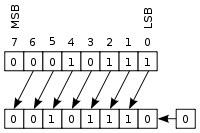
\includegraphics[scale=0.66]{14_bitfields/200px-Rotate_left_logically.png}
\caption{\IFRU{Как работает инструкция \SHL\protect\footnotemark}
{How \SHL instruction works\protect\footnotemark}}
\end{figure}

\footnotetext{\IFRU{иллюстрация взята из}{illustration taken from} wikipedia}

\index{x86!\Instructions!AND}
\IFRU{Макрос \TT{IS\_SET} на самом деле это операция логического И (\IT{AND}) 
и она возвращает $0$ если бита там нет, 
либо эту же битовую маску, если бит там есть. 
В \CCpp, конструкция \TT{if()} срабатывает, если выражение внутри её не ноль, пусть хоть $123456$, 
поэтому все будет работать.}
{The \TT{IS\_SET} macro is in fact logical and operation (\IT{AND}) 
and it returns $0$ if specific bit is absent there,
or bit mask, if the bit is present.
\IT{if()} operator triggered in \CCpp if expression in it is not a zero, it might be even $123456$, that is why
it always working correctly.}

\subsubsection{x86}

\IFRU{Компилируем}{Let's compile} (MSVC 2010):

\lstinputlisting[caption=MSVC 2010]{\IFRU{14_bitfields/shifts_MSVC_ru.asm}{14_bitfields/shifts_MSVC_en.asm}}

\IFRU{Вот так работает SHL (\IT{SHift Left})}{That's how SHL (\IT{SHift Left}) working}.

\IFRU{Скомпилируем то же и в}{Let's compile it in} GCC 4.4.1:

\lstinputlisting[caption=GCC 4.4.1]{14_bitfields/shifts_gcc.asm}

\IFRU{Инструкции сдвига также активно применяются при делении или умножении 
на числа-степени двойки ($1$, $2$, $4$, $8$, итд).}
{Shift instructions are often used in division and multiplications by power of two numbers 
($1$, $2$, $4$, $8$, etc).}

\IFRU{Например:}{For example:}

\begin{lstlisting}
unsigned int f(unsigned int a)
{
	return a/4;
};
\end{lstlisting}

\IFRU{Имеем в итоге}{We got} (MSVC 2010):

\begin{lstlisting}[caption=MSVC 2010]
_a$ = 8							; size = 4
_f	PROC
	mov	eax, DWORD PTR _a$[esp-4]
	shr	eax, 2
	ret	0
_f	ENDP
\end{lstlisting}

\label{SHR}
\index{x86!\Instructions!SHR}
\IFRU{Инструкция \SHR (\IT{SHift Right}) в данном примере сдвигает число на 2 бита вправо. 
При этом, освободившиеся два бита слева (т.е., самые 
старшие разряды), выставляются в нули. А самые младшие 2 бита выкидываются. 
Фактически, эти два выкинутых бита ~--- остаток от деления.}
{\SHR (\IT{SHift Right}) instruction in this example is shifting a number by 2 bits right.
Two freed bits at left (e.g., two most significant bits) are set to zero.
Two least significant bits are dropped.
In fact, these two dropped bits ~--- division operation remainder.}

\index{x86!\Instructions!SHL}
\IFRU{Инструкция \SHR работает так же как и \SHL, только в другую сторону.}
{\SHR instruction works just like as \SHL but in other direction.}

\begin{figure}[ht!]
\centering
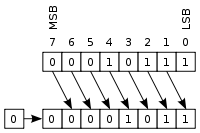
\includegraphics[scale=0.66]{14_bitfields/200px-Rotate_right_logically.png}
\caption{\IFRU{Как работает инструкция \SHR\protect\footnotemark}
{How \SHR instruction works\protect\footnotemark}}
\end{figure}

\footnotetext{\IFRU{иллюстрация взята из}{illustration taken from} wikipedia}

\label{division_by_shifting}
\IFRU{Для того, чтобы это проще понять, представьте себе десятичную систему счисления и число $23$. 
$23$ можно разделить на $10$ просто откинув последний разряд ($3$ ~--- это остаток от деления). 
После этой операции останется $2$ как частное
\footnote{результат деления}.}
{It can be easily understood if to imagine decimal numeral system and number $23$.
$23$ can be easily divided by $10$ just by dropping last digit ($3$ ~--- is division remainder). 
$2$ is leaving after operation as a quotient
\footnote{division result}.}

\IFRU{Так и с умножением. Умножить на $4$ это просто сдвинуть число на 2 бита влево, 
вставив 2 нулевых бита справа (как два самых младших бита). 
Это как умножить $3$ на $100$ ~--- нужно просто дописать два нуля справа.}
{The same story about multiplication.
Multiplication by $4$ is just shifting the number to the left by 2 bits,
while inserting 2 zero bits at right (as the last two bits).
It's just like to multiply $3$ by $100$ ~--- we need just to add two zeroes at the right.}




\subsubsection{ARM + \OptimizingXcode + \ARMMode}

\begin{lstlisting}[caption=\OptimizingXcode + \ARMMode]
                MOV             R1, R0
                MOV             R0, #0
                MOV             R2, #1
                MOV             R3, R0
loc_2E54
                TST             R1, R2,LSL R3 ; set flags according to R1 & (R2<<R3)
                ADD             R3, R3, #1    ; R3++
                ADDNE           R0, R0, #1    ; if ZF flag is cleared by TST, R0++
                CMP             R3, #32
                BNE             loc_2E54
                BX              LR
\end{lstlisting}

\index{ARM!\Instructions!TST}
\TT{TST} \IFRU{это то же что и}{is the same things as} \TEST \IFRU{в}{in} x86.

\index{ARM!Optional operators!LSL}
\index{ARM!Optional operators!LSR}
\index{ARM!Optional operators!ASR}
\index{ARM!Optional operators!ROR}
\index{ARM!Optional operators!RRX}
\index{ARM!\Instructions!MOV}
\index{ARM!\Instructions!TST}
\index{ARM!\Instructions!CMP}
\index{ARM!\Instructions!ADD}
\index{ARM!\Instructions!SUB}
\index{ARM!\Instructions!RSB}
\IFRU{Как я уже указывал}{As I mentioned before}~\ref{shifts_in_ARM_mode}, 
\IFRU{в режиме ARM нет отдельной инструкции для сдвигов.}
{there are no separate shifting instructions in ARM mode.}
\IFRU{Однако, модификаторами}{However, there are modifiers} 
LSL (\IT{Logical Shift Left}), 
LSR (\IT{Logical Shift Right}), 
ASR (\IT{Arithmetic Shift Right}), 
ROR (\IT{Rotate Right}) \IFRU{и}{and} 
RRX (\IT{Rotate Right with Extend}) \IFRU{можно дополнять некоторые инструкции, такие как}
{, which may be added to such instructions as} \MOV, \TT{TST},
\CMP, \ADD, \SUB, \TT{RSB}\footnote{\DataProcessingInstructionsFootNote}.

\IFRU{Эти модифицкаторы указывают, как сдвигать второй операнд, и на сколько.}
{These modificators are defines, how to shift second operand and by how many bits.}

\index{ARM!Optional operators!LSL}
\IFRU{Таким образом, инструкция }{Thus} \TT{``TST R1, R2,LSL R3''} 
\IFRU{здесь работает как}{instruction works here as} $R1 \land (R2 \ll R3)$.

\subsubsection{ARM + \OptimizingXcode + \ThumbTwoMode}

\index{ARM!\Instructions!LSL.W}
\index{ARM!\Instructions!LSL}
\IFRU{Почти такое же}{Almost the same}, 
\IFRU{только здесь применяется пара инструкций}{but here are two} 
\TT{LSL.W}/\TT{TST} 
\IFRU{вместо одной}{instructions are used instead of single} 
\TT{TST},
\IFRU{ведь в режиме thumb нельзя добавлять указывать модификатор}{becase, in thumb mode, it's not
possible to define} \TT{LSL} \IFRU{прямо в}{modifier right in} \TT{TST}.

\begin{lstlisting}
                MOV             R1, R0
                MOVS            R0, #0
                MOV.W           R9, #1
                MOVS            R3, #0
loc_2F7A
                LSL.W           R2, R9, R3
                TST             R2, R1
                ADD.W           R3, R3, #1
                IT NE
                ADDNE           R0, #1
                CMP             R3, #32
                BNE             loc_2F7A
                BX              LR
\end{lstlisting}





\subsection{\IFRU{Пример вычисления CRC32}{CRC32 calculation example}}
\index{CRC32}

\newcommand{\URLCRCSRC}{\url{http://burtleburtle.net/bob/c/crc.c}}

\IFRU{Это распространенный табличный способ вычисления хеша алгоритмом 
CRC32\footnote{Исходник взят тут: \URLCRCSRC}.}
{This is very popular table-based CRC32 hash calculation 
method\footnote{Source code was taken here: \URLCRCSRC}.}

\lstinputlisting{14_bitfields/CRC.c}

\index{\CLanguageElements!for}
\IFRU{Нас интересует функция \TT{crc()}. 
Кстати, обратите внимание на два инициализатора в выражении \TT{for()}: \TT{hash=len, i=0}. 
Стандарт \CCpp, конечно, допускает это. А в итоговом коде, вместо одной операции инициализации цикла, будет две.}
{We are interesting in the \TT{crc()} function only.
By the way, pay attention to two loop initializers in the \TT{for()} statement: \TT{hash=len, i=0}.
\CCpp standard allows this, of course.
Emitted code will contain two operations in loop initialization part
instead of usual one.}

\IFRU{Компилируем в MSVC с оптимизацией (\Ox). 
Для краткости, я приведу только функцию \TT{crc()}, с некоторыми комментариями.}
{Let's compile it in MSVC with optimization (\Ox).
For the sake of brevity, only \TT{crc()} function is listed here, with my comments.}

\lstinputlisting{\IFRU{14_bitfields/CRC_2_ru.asm}{14_bitfields/CRC_2_en.asm}}

\IFRU{Попробуем то же самое в GCC 4.4.1 с опцией \Othree:}
{Let's try the same in GCC 4.4.1 with \Othree option:}

\lstinputlisting{\IFRU{14_bitfields/CRC_gcc_O3_ru.asm}{14_bitfields/CRC_gcc_O3_en.asm}}

\index{x86!\Instructions!NOP}
\index{x86!\Instructions!LEA}
\IFRU{GCC немного выровнял начало тела цикла по 8-байтной границе, для этого добавил 
\NOP и \TT{lea esi, [esi+0]} (что тоже \IT{холостая операция}). 
Подробнее об этом смотрите в разделе о npad~\ref{sec:npad}.}
{GCC aligned loop start on a 8-byte border by adding \NOP and \TT{lea esi, [esi+0]} (that is \IT{idle operation} too).
Read more about it in npad section~\ref{sec:npad}.}




\section{\IFRU{Структуры}{Structures}}

\IFRU{В принципе, структура в \CCpp это, с некоторыми допущениями, просто всегда лежащий рядом, 
и в той же последовательности, набор переменных, не обязательно одного типа.}
{It can be defined that \CCpp structure, with some assumptions, just a set of variables, always stored
in memory together, not necessary of the same type.}

\subsection{\IFRU{Пример SYSTEMTIME}{SYSTEMTIME example}}

\newcommand{\FNSYSTEMTIME}{\footnote{\href{http://msdn.microsoft.com/en-us/library/ms724950(VS.85).aspx}{MSDN: SYSTEMTIME structure}}}

\IFRU{Возьмем, к примеру, структуру SYSTEMTIME\FNSYSTEMTIME{} из win32 описывающую время.}
{Let's take SYSTEMTIME\FNSYSTEMTIME{} win32 structure describing time.}

\IFRU{Она объявлена так:}{That's how it's defined:}

\begin{lstlisting}[caption=WinBase.h]
typedef struct _SYSTEMTIME {
  WORD wYear;
  WORD wMonth;
  WORD wDayOfWeek;
  WORD wDay;
  WORD wHour;
  WORD wMinute;
  WORD wSecond;
  WORD wMilliseconds;
} SYSTEMTIME, *PSYSTEMTIME;
\end{lstlisting}

\IFRU{Пишем на Си функцию для получения текущего системного времени:}
{Let's write a C function to get current time:}

\lstinputlisting{15_structs/systemtime.c}

\IFRU{Что в итоге}{We got} (MSVC 2010):

\lstinputlisting[caption=MSVC 2010]{15_structs/systemtime.asm}

\IFRU{Под структуру в стеке выделено 16 байт ~--- именно столько будет \TT{sizeof(WORD)*8}
(в структуре 8 переменных с типом WORD).}
{16 bytes are allocated for this structure in local stack ~--- that's exactly \TT{sizeof(WORD)*8}
(there are 8 WORD variables in the structure).}

\newcommand{\FNMSDNGST}{\footnote{\href{http://msdn.microsoft.com/en-us/library/ms724390(VS.85).aspx}{MSDN: GetSystemTime function}}}

\IFRU{Обратите внимание на тот факт что структура начинается с поля \TT{wYear}. 
Можно сказать что в качестве аргумента для \TT{GetSystemTime()}\FNMSDNGST передается указатель на структуру 
SYSTEMTIME, но можно также сказать, что передается указатель на поле \TT{wYear}, 
что одно и тоже! 
\TT{GetSystemTime()} пишет текущий год в тот WORD на который указывает переданный указатель, 
затем сдвигается на 2 байта вправо, пишет текущий месяц, итд, итд.}
{Pay attention to the fact the structure beginning with \TT{wYear} field.
It can be said, an pointer to SYSTEMTIME structure is passed to \TT{GetSystemTime()}\FNSYSTEMTIME,
but it's also can be said, pointer to \TT{wYear} field is passed, and that's the same!
\TT{GetSystemTime()} writting current year to the WORD pointer pointing to, then shifting 2 bytes
ahead, then writting current month, etc, etc.}

\IFRU{Тот факт что поля структуры это просто переменные расположенные рядом, 
я могу проиллюстрировать следующим образом.}
{The fact that structure fields are just variables located side-by-side, 
I can illustrate by the following method.}
\IFRU{Глядя на описание структуры}{Keeping in ming} \TT{SYSTEMTIME}\IFRU{, я могу переписать этот простой пример так:}
{ structure description, I can rewrite this simple example like this:}

\lstinputlisting{15_structs/systemtime2.c}

\IFRU{Компилятор немного поворчит:}{Compiler will warn us:}

\begin{lstlisting}
systemtime2.c(7) : warning C4133: 'function' : incompatible types - from 'WORD [8]' to 'LPSYSTEMTIME'
\end{lstlisting}

\IFRU{Тем не менее, выдаст такой код}{But nevertheless, it will produce this code}:

\lstinputlisting[caption=MSVC 2010]{15_structs/systemtime2.asm}

\IFRU{И это работает так же}{And it works just as the same}!

\IFRU{Любопытно что результат на ассемблере неотличим от предыдущего}{It's very interesting fact that
result in assembly form cannot be distinguished from the result of previous compilation}.
\IFRU{Таким образом, глядя на этот код, 
никогда нельзя сказать с уверенностью, была ли там объявлена структура, либо просто набор переменных.}
{So by looking at this code, one cannot say for sure, was there structure declared, or just pack of variables.} 

\IFRU{Тем не менее, никто в здравом уме делать так не будет}{Nevertheless, no one will do it in sane state of mind}.
\IFRU{Потому что это неудобно}{Because it's not handy}. 
\IFRU{К тому же, иногда, поля в структуре могут меняться разработчиками, 
переставляться местами, итд}{Also, structure fields may be changed by developers, swapped, etc}.



\subsection{\IFRU{Выделяем место для структуры через malloc()}{Let's allocate place for structure using malloc()}}

\IFRU{Однако, бывает и так, что проще хранить структуры не в стеке а в куче\footnote{heap}:}
{However, sometimes it's simpler to place structures not in local stack, but in heap:}

\lstinputlisting{15_structs/systemtime_malloc.c}

\IFRU{Скомпилируем на этот раз с оптимизацией (\Ox) чтобы было проще увидеть то, что нам нужно.}
{Let's compile it now with optimization (\Ox) so to easily see what we need.}

\lstinputlisting[caption=\Optimizing MSVC]{15_structs/systemtime_malloc.asm}

\index{\CStandardLibrary!malloc()}
\IFRU{Итак, \TT{sizeof(SYSTEMTIME) = 16}, именно столько байт выделяется при помощи \TT{malloc()}. 
Она возвращает указатель на только что выделенный блок памяти в \EAX, который копируется в \ESI. 
Win32 функция \TT{GetSystemTime()} обязуется сохранить состояние \ESI, 
поэтому здесь оно нигде не сохраняется и продолжает использоваться после вызова \TT{GetSystemTime()}.}
{So, \TT{sizeof(SYSTEMTIME) = 16}, that's exact number of bytes to be allocated by \TT{malloc()}.
It return the pointer to freshly allocated memory block in \EAX, which is then moved into \ESI.
\TT{GetSystemTime()} win32 function undertake to save \ESI value, 
and that's why it is not saved here and continue to be used after \TT{GetSystemTime()} call.}

\index{x86!\Instructions!MOVZX}
\IFRU{
Новая инструкция ~--- \MOVZX (\IT{Move with Zero eXtent}). 
Она нужна почти там же где и \MOVSX, 
только всегда очищает остальные биты в $0$. Дело в том что \printf требует 32-битный тип \Tint, 
а в структуре лежит WORD ~--- это 16-битный беззнаковый тип. Поэтому копируя значение из WORD в \Tint, 
нужно очистить биты от 16 до 31, иначе там будет просто случайный мусор, оставшийся от предыдущих действий 
с регистрами.}
{New instruction ~--- \MOVZX (\IT{Move with Zero eXtent}).
It may be used almost in those cases as \MOVSX, but, it clearing other bits to $0$.
That's because \printf require 32-bit \Tint, but we got WORD in structure ~--- that's 16-bit unsigned type.
That's why by copying value from WORD into \Tint{}, bits from 16 to 31 should be cleared, 
because there will be random noise otherwise, leaved from previous operations on registers.}

\IFRU{В этом примере я тоже могу представить структуру как массив WORD-ов}{In this example, I can represent
structure as array of WORD-s}:

\lstinputlisting{15_structs/systemtime_malloc2.c}

\IFRU{Получим такое}{We got}:

\lstinputlisting[caption=\Optimizing MSVC]{15_structs/systemtime_malloc2.asm}

\IFRU{И снова мы получаем идетичный код, неотличимый от предыдущего}{Again, we got a code that cannot be distinguished
from previous}.
\IFRU{Но и снова я должен отметить, что в реальности так лучше не делать}{And again I should note, one shouldn't do
this in practice}.



\subsection{struct tm}

\subsubsection{Linux}

\IFRU{В Линуксе, для примера, возьем структуру \TT{tm} из \TT{time.h}:}
{As of Linux, let's take \TT{tm} structure from \TT{time.h} for example:}

\lstinputlisting{15_structs/GCC_tm.c}

\IFRU{Компилируем при помощи}{Let's compile it in} GCC 4.4.1:

\IFRU{\lstinputlisting[caption=GCC 4.4.1]{15_structs/GCC_tm_ru.asm}}{\lstinputlisting{15_structs/GCC_tm_en.asm}}

\IFRU{К сожалению, по какой-то причине, \IDA не сформировала названия локальных переменных в стеке. 
Но так как мы уже опытные реверсеры :-) то можем обойтись и без этого в таком простом примере.}
{Somehow, \IDA didn't created local variables names in local stack.
But since we already experienced reverse engineers :-) we may do it without this information in 
this simple example.}

\IFRU{Обратите внимание на \TT{lea edx, [eax+76Ch]} ~--- эта инструкция прибавляет $0x76C$ к \EAX, 
но не модифицирует флаги. См. также соответствующий раздел об инструкции \LEA{}~\ref{sec:LEA}.}
{Please also pay attention to \TT{lea edx, [eax+76Ch]} ~--- this instruction just adding $0x76C$ to \EAX,
but not modify any flags. See also relevant section about \LEA{}~\ref{sec:LEA}.}

Чтобы проиллюстрировать то что структура это просто набор переменных лежащих в одном месте, переделаем немного
пример, заглянув предварительно в файл time.h:

\begin{lstlisting}[caption=time.h]
struct tm
{
  int	tm_sec;
  int	tm_min;
  int	tm_hour;
  int	tm_mday;
  int	tm_mon;
  int	tm_year;
  int	tm_wday;
  int	tm_yday;
  int	tm_isdst;
};
\end{lstlisting}

\lstinputlisting{15_structs/GCC_tm2.c}

Обратите внимание на то что в \TT{localtime\_r} передается указатель именно на \TT{tm\_sec}, 
т.е., на первый элемент ``структуры''.

В итоге, и этот компилятор поворчит:

\begin{lstlisting}[caption=GCC 4.7.3]
GCC_tm2.c: In function 'main':
GCC_tm2.c:11:5: warning: passing argument 2 of 'localtime_r' from incompatible pointer type [enabled by default]
In file included from GCC_tm2.c:2:0:
/usr/include/time.h:59:12: note: expected 'struct tm *' but argument is of type 'int *'
\end{lstlisting}

Тем не менее, сгенерирует такоу:

\lstinputlisting[caption=GCC 4.7.3]{15_structs/GCC_tm2.asm}

Этот код почти идентичен уже рассмотренному, и нельзя сказать, была ли структура
в оригинальном исходном коде либо набор переменных.

И это работает. Однако, в реальности так лучше не делать. Обычно, компилятор располагает переменные в локальном
стеке в том же порядке, в котором они объявляются в функции. Тем не менее, никакой гарантии нет.

Кстати, какой-нибудь другой компилятор может предупредить, что переменные \TT{tm\_year}, \TT{tm\_mon}, \TT{tm\_mday},
\TT{tm\_hour}, \TT{tm\_min}, но не \TT{tm\_sec}, используются без инициализации. 
Действительно, ведь компилятор не знает
что они будут заполнены при вызове функции \TT{localtime\_r()}.

Я выбрал именно этот пример для иллюстрации, потому что члены структуры имеют тип \Tint, а члены структуры
\TT{SYSTEMTIME} ~--- 16-битные \TT{WORD}, и если их объявлять так же, то они будут выровнены по 32-битной границе 
и ничего не выйдет (потому что \TT{GetSystemTime()} заполнит их неверно). Читайте об этом в следующей секции
``\StructurePackingSectionName''.

\index{\SyntacticSugar}
Так что, структура это просто набор переменных лежащих в одном месте, рядом. Я мог бы сказать что структура
это такой синтаксический сахар, заставляющий компилятор удерживать их в одном месте. Впрочем, я не специалист
по языкам программирования, так что, скорее всего, ошибаюсь с этим термином.
Кстати, когда-то, в очень ранних версиях Си (перед 1972) структур не 
было вовсе\cite{Ritchie:1993:DCL:155360.155580}.

\subsubsection{ARM + \OptimizingKeil + \ThumbMode}

Этот же пример:

\lstinputlisting[caption=\OptimizingKeil + \ThumbMode]{15_structs/tm_ARM_keil_thumb.asm}

\subsubsection{ARM + \OptimizingXcode + \ThumbTwoMode}

\IDA ``узнала'' структуру tm (потому что \IDA ``знает'' типы аргументов библиотечных функций, 
таких как \TT{localtime\_r()}), поэтому показала здесь обращения к элементам структуры.

\lstinputlisting[caption=\OptimizingXcode + \ThumbTwoMode]{15_structs/tm_ARM_xcode_thumb.asm}



\subsection{\StructurePackingSectionName}

\IFRU{Достаточно немаловажный момент, это упаковка полей в структурах\footnote{См.также: \URLWPDA}.}
{One important thing is fields packing in structures\footnote{See also: \URLWPDA}.}

\IFRU{Возьмем простой пример:}{Let's take a simple example:}

\lstinputlisting{15_structs/packing.c}

\IFRU{Как видно, мы имеем два поля \Tchar (занимающий один байт) и еще два ~--- \Tint (по 4 байта).}
{As we see, we have two \Tchar fields (each is exactly one byte) and two more ~--- \Tint (each - 4 bytes).}

\subsubsection{x86}

\IFRU{Компилируется это все в:}{That's all compiling into:}

\lstinputlisting{15_structs/packing.asm}

\IFRU{Мы видим здесь что адрес каждого поля в структуре выравнивается по 4-байтной границе. 
Так что каждый \Tchar здесь занимает те же 4 байта что и \Tint. Зачем? 
Затем что процессору удобнее обращаться по таким адресам и кешировать данные из памяти.}
{As we can see, each field's address is aligned on a 4-bytes border.
That's why each \Tchar occupies 4 bytes here (like \Tint). Why?
Thus it is easier for CPU to access memory at aligned addresses and to cache data from it.}

\IFRU{Но это не экономично по размеру данных.}{However, it is not very economical in size sense.}

\IFRU{Попробуем скомпилировать тот же исходник с опцией}{Let's try to compile it with option} (\TT{/Zp1}) 
(\IT{/Zp[n] pack structs on n-byte boundary}).

\lstinputlisting[caption=MSVC /Zp1]{15_structs/packing_msvc_Zp1.asm}

\IFRU{Теперь структура занимает 10 байт и все \Tchar занимают по байту. Что это дает? 
Экономию места. Недостаток ~--- процессор будет обращаться к этим полям не так эффективно 
по скорости как мог бы.}
{Now the structure takes only 10 bytes and each \Tchar value takes 1 byte. What it give to us?
Size economy. And as drawback ~--- CPU will access these fields without maximal performance it can.}

\IFRU{Как нетрудно догадаться, если структура используется много в каких исходниках и объектных файлах, 
все они должны быть откомпилированы с одним и тем же соглашением об упаковке структур.}
{As it can be easily guessed, if the structure is used in many source and object files,
all these should be compiled with the same convention about structures packing.}

\newcommand{\FNURLMSDNZP}{\footnote{\href{http://msdn.microsoft.com/en-us/library/ms253935.aspx}
{MSDN: Working with Packing Structures}}}
\newcommand{\FNURLGCCPC}{\footnote{\href{http://gcc.gnu.org/onlinedocs/gcc/Structure_002dPacking-Pragmas.html}
{Structure-Packing Pragmas}}}

\IFRU{Помимо ключа MSVC \TT{/Zp}, указывающего, по какой границе упаковывать поля структур, есть также 
опция компилятора \TT{\#pragma pack}, её можно указывать прямо в исходнике. 
Это справедливо и для MSVC\FNURLMSDNZP и GCC\FNURLGCCPC{}.}
{Aside from MSVC \TT{/Zp} option which set how to align each structure field, here is also
\TT{\#pragma pack} compiler option, it can be defined right in source code.
It is available in both MSVC\FNURLMSDNZP and GCC\FNURLGCCPC{}.}

\IFRU{Давайте теперь вернемся к \TT{SYSTEMTIME}, которая состоит из 16-битных полей. 
Откуда наш компилятор знает что их надо паковать по однобайтной границе?}
{Let's back to the \TT{SYSTEMTIME} structure consisting in 16-bit fields.
How our compiler know to pack them on 1-byte alignment method?}

\IFRU{В файле \TT{WinNT.h} попадается такое:}{\TT{WinNT.h} file has this:}

\begin{lstlisting}[caption=WinNT.h]
#include "pshpack1.h"
\end{lstlisting}

\IFRU{И такое:}{And this:}

\begin{lstlisting}[caption=WinNT.h]
#include "pshpack4.h"                   // 4 byte packing is the default
\end{lstlisting}

\IFRU{Сам файл PshPack1.h выглядит так:}{The file PshPack1.h looks like:}

\begin{lstlisting}[caption=PshPack1.h]
#if ! (defined(lint) || defined(RC_INVOKED))
#if ( _MSC_VER >= 800 && !defined(_M_I86)) || defined(_PUSHPOP_SUPPORTED)
#pragma warning(disable:4103)
#if !(defined( MIDL_PASS )) || defined( __midl )
#pragma pack(push,1)
#else
#pragma pack(1)
#endif
#else
#pragma pack(1)
#endif
#endif /* ! (defined(lint) || defined(RC_INVOKED)) */
\end{lstlisting}

\IFRU{Собственно, так и задается компилятору, как паковать объявленные после \TT{\#pragma pack} структуры.}
{That's how compiler will pack structures defined after \TT{\#pragma pack}.}

\subsubsection{ARM + \OptimizingKeil + \ThumbMode}

\lstinputlisting[caption=\OptimizingKeil + \ThumbMode]{15_structs/packing_Keil_thumb.asm}

\IFRU{Как мы помним, здесь передается не указатель на структуру, а сама структура, а так как в ARM первые 4 аргумента
функции передаются через регистры, то поля структуры передаются через}
{As we may recall, here a structure passed instead of pointer to structure,
and since first 4 function arguments in ARM are passed via registers,
so then structure fields are passed via} \TT{R0-R3}.

\index{ARM!\Instructions!LDRB}
\index{x86!\Instructions!MOVSX}
\IFRU{Инструкция }\TT{LDRB} \IFRU{загружает один байт из памяти и расширяет до 32-бит учитывая знак.}
{loads one byte from memory and extending it to 32-bit, taking into account its sign.}
\IFRU{Это похоже на инструкцию}{This is similar to} \MOVSX \IFRU{в}{instruction in} x86.
\IFRU{Она здесь применяется дла загрузки полей}{Here it is used for loading fields} $a$ \AndENRU $c$ 
\IFRU{из структуры}{from structure}.

\index{Function epilogue}
\IFRU{Еще что бросается в глаза, так это то что вместо эпилога функции, переход на эпилог другой функции!}
{One more thing we spot easily, instead of function epilogue, here is jump to another function's epilogue!}
\IFRU{Действительно, то была совсем другая, не относящаяся к этой, функция, однако, она имела точно такой же
эпилог}{Indeed, that was another function, not related in any way to our function, however, it has exactly
the same epilogue} 
(\IFRU{видимо, тоже хранила в стеке 5 локальных переменных}{probably because, it hold 5 local variables too} 
($5*4=0x14$)).
\IFRU{К тому же, она находится рядом (обратите внимание на адреса).}
{Also it is located nearly (take a look on addresses).}
\IFRU{Действительно, нет никакой разницы, какой эпилог исполнять, если он работает так же как нам нужно.}
{Indeed, there are no difference, which epilogue to execute, if it works just as we need.}
\IFRU{Keil решил сделать так, вероятно, из-за экономии.}{Apparently, Keil decides to do this by a reason of economy.}
\IFRU{Эпилог занимает 4 байта, а переход ~--- только 2.}{Epilogue takes 4 bytes while jump ~--- only 2.}

\subsubsection{ARM + \OptimizingXcode + \ThumbTwoMode}

\lstinputlisting[caption=\OptimizingXcode + \ThumbTwoMode]{15_structs/packing_Xcode_thumb.asm}

\index{ARM!\Instructions!SXTB}
\index{x86!\Instructions!MOVSX}
\TT{SXTB} (\IT{Signed Extend Byte}) \IFRU{это так же аналог}{is analogous to} \MOVSX \In 
x86\IFRU{, только работает не с памятью, а с регистром.}{ as well, but works not with memory, but with register.}
\IFRU{Всё остальное ~--- так же.}{All the rest ~--- just the same.}



\subsection{\IFRU{Вложенные структуры}{Nested structures}}

\IFRU{Теперь, как насчет ситуаций, когда одна структура определяет внутри себя еще одну структуру?}
{Now what about situations when one structure defines another structure inside?}

\lstinputlisting{15_structs/nested.c}

\dots \IFRU{в этом случае, оба поля \TT{inner\_struct} просто будут располагаться между полями a,b и d,e в 
\TT{outer\_struct}.}
{in this case, both \TT{inner\_struct} fields will be placed between a,b and d,e fields of
\TT{outer\_struct}.}

\IFRU{Компилируем}{Let's compile} (MSVC 2010):

\lstinputlisting[caption=MSVC 2010]{15_structs/nested_msvc.asm}

\IFRU{Очень любопытный момент в том, что глядя на этот код на ассемблере, мы даже не видим, 
что была использована какая-то еще другая структура внутри этой!
Так что, пожалуй, можно сказать, что все вложенные структуры в итоге разворачиваются в одну, \IT{линейную} 
или \IT{одномерную} структуру.}
{One curious point here is that by looking onto this assembly code, we do not even see that
another structure was used inside of it!
Thus, we would say, nested structures are finally unfolds into \IT{linear} or \IT{one-dimensional} structure.}

\IFRU{Конечно, если заменить объявление \TT{struct inner\_struct c;} на \TT{struct inner\_struct *c;} 
(объявляя таким образом указатель), ситауция будет совсем иная.}
{Of course, if to replace \TT{struct inner\_struct c;} declaration to \TT{struct inner\_struct *c;} 
(thus making a pointer here) situation will be significally different.}



\subsection{\IFRU{Работа с битовыми полями в структуре}{Bit fields in structure}}

\subsubsection{\IFRU{Пример CPUID}{CPUID example}}

\IFRU{Язык \CCpp позволяет укзывать, сколько именно бит отвести для каждого поля структуры. 
Это удобно если нужно экономить место в памяти. К примеру, для переменной типа \Tbool достаточно одного бита.
Но, это не очень удобно, если нужна скорость.}
{\CCpp language allow to define exact number of bits for each structure fields.
It is very useful if one needs to save memory space. 
For example, one bit is enough for variable of \Tbool type.
But of course, it is not rational if speed is important.}

\newcommand{\FNCPUID}{\footnote{\url{http://en.wikipedia.org/wiki/CPUID}}}

\index{x86!\Instructions!CPUID}
\IFRU{Рассмотрим пример с инструкцией \CPUID\FNCPUID. 
Эта инструкция возвращает информацию о том, какой процессор имеется в наличии и какие фичи он имеет.}
{Let's consider \CPUID\FNCPUID instruction example.
This instruction returning information about current CPU and its features.}

\IFRU{Если перед исполнением инструкции в \EAX будет 1, 
то \CPUID вернет упакованную в \EAX такую информацию о процессоре:}
{If the \EAX is set to 1 before instruction execution, 
\CPUID will return this information packed into the \EAX register:}

\begin{center}
\begin{tabular}{ | l | l | }
\hline
3:0 & Stepping \\
7:4 & Model \\
11:8 & Family \\
13:12 & Processor Type \\
19:16 & Extended Model \\
27:20 & Extended Family \\
\hline
\end{tabular}
\end{center}

\newcommand{\FNGCCAS}{\footnote{\href{http://www.ibiblio.org/gferg/ldp/GCC-Inline-Assembly-HOWTO.html}
{\IFRU{Подробнее о встроенном ассемблере GCC}{More about internal GCC assembler}}}}

\IFRU{MSVC 2010 имеет макрос для \CPUID, а GCC 4.4.1 ~--- нет. 
Поэтому для GCC сделаем эту функцию сами, используя его встроенный ассемблер\FNGCCAS.}
{MSVC 2010 has \CPUID macro, but GCC 4.4.1 ~--- has not.
So let's make this function by yourself for GCC with the help of its built-in assembler\FNGCCAS.}

\lstinputlisting{15_structs/CPUID.c}

\IFRU{После того как \CPUID заполнит \EAX/\EBX/\ECX/\EDX, у нас они отразятся в массиве \TT{b[]}. 
Затем, мы имеем указатель на структуру \TT{CPUID\_1\_EAX}, и мы указываем его на значение 
\EAX из массива \TT{b[]}.}
{After \CPUID will fill \EAX/\EBX/\ECX/\EDX, these registers will be reflected in the \TT{b[]} array.
Then, we have a pointer to the \TT{CPUID\_1\_EAX} structure and we point it to the value in the \EAX from \TT{b[]} array.}

\IFRU{Иными словами, мы трактуем 32-битный \Tint как структуру.}
{In other words, we treat 32-bit \Tint value as a structure.}

\IFRU{Затем мы читаем из структуры.}{Then we read from the stucture.}

\IFRU{Компилируем в MSVC 2008 с опцией \Ox}{Let's compile it in MSVC 2008 with \Ox option}:

\lstinputlisting[caption=\Optimizing MSVC 2008]{15_structs/CPUID_msvc_Ox.asm}

\index{x86!\Instructions!SHR}
\IFRU{Инструкция \TT{SHR} сдвигает значение из \EAX на то количество бит, 
которое нужно \IT{пропустить}, то есть, мы игнорируем некоторые биты \IT{справа}.}
{\TT{SHR} instruction shifting value in the \EAX register by number of bits should be
\IT{skipped}, e.g., we ignore a bits \IT{at right}.}

\index{x86!\Instructions!AND}
\IFRU{А инструкция \ANDIns очищает биты \IT{слева} которые нам не нужны, или же, говоря иначе, 
она оставляет по маске только те биты в \EAX, которые нам сейчас нужны.}
{\ANDIns instruction clears bits not needed \IT{at left}, or, in other words, 
leaves only those bits in the \EAX register we need now.}

\IFRU{Попробуем GCC 4.4.1 с опцией \Othree.}{Let's try GCC 4.4.1 with \Othree option.}

\lstinputlisting[caption=\Optimizing GCC 4.4.1]{15_structs/CPUID_gcc_O3.asm}

\IFRU{Практически, то же самое. Единственное что стоит отметить это то, что GCC решил зачем-то объеденить 
вычисление \TT{extended\_model\_id} и \TT{extended\_family\_id} в один блок, 
вместо того чтобы вычислять их перед соответствующим вызовом \printf.}
{Almost the same. The only thing worth noting is that GCC somehow united calculation of
\TT{extended\_model\_id} and \TT{extended\_family\_id} into one block,
instead of calculating them separately, before corresponding each \printf call.}

\subsubsection{\WorkingWithFloatAsWithStructSubSubSectionName}
\label{sec:floatasstruct}

\IFRU{Как уже раннее указывалось в секции о FPU~\ref{sec:FPU}, и \Tfloat и \Tdouble содержат в себе знак, 
мантиссу и экспоненту. 
Однако, можем ли мы работать с этими полями напрямую? Попробуем с \Tfloat.}
{As it was already noted in section about FPU~\ref{sec:FPU}, both \Tfloat and \Tdouble types consisted of sign,
significand (or fraction) and exponent.
But will we able to work with these fields directly? Let's try with \Tfloat.}

\index{IEEE 754}
\index{float}
\begin{figure}[ht!]
\centering
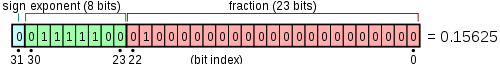
\includegraphics[scale=0.66]{15_structs/500px-Float_example.png}
\caption{\IFRU{Формат значения float\protect\footnotemark}
{float value format\protect\footnotemark}}
\end{figure}

\footnotetext{\IFRU{иллюстрация взята из}{illustration taken from} wikipedia}

\lstinputlisting{15_structs/float_en.c}

\IFRU{Структура \TT{float\_as\_struct} занимает в памяти столько же места сколько и \Tfloat, 
то есть 4 байта или 32 бита.}
{\TT{float\_as\_struct} structure occupies as much space is memory as \Tfloat, e.g., 4 bytes or 32 bits.}

\IFRU{Далее мы выставляем во входящем значении отрицательный знак, 
а также прибавляя двойку к экспоненте, мы тем 
самым умножаем всё значение на \TT{$2^2$}, то есть на 4.}
{Now we setting negative sign in input value and also by addding 2 to exponent we thereby multiplicating
the whole number by \TT{$2^2$}, e.g., by 4.}

\IFRU{Компилируем в MSVC 2008 без оптимизации:}{Let's compile in MSVC 2008 without optimization:}

\lstinputlisting[caption=\NonOptimizing MSVC 2008]
{\IFRU{15_structs/float_msvc_ru.asm}{15_structs/float_msvc_en.asm}}

\IFRU{Слекга избыточно. В версии скомпилированной с флагом \Ox нет вызовов \TT{memcpy()}, 
там работа происходит сразу с переменной f. Но по неоптимизированной версии будет проще понять.}
{Redundant for a bit.
If it is compiled with \Ox flag there is no \TT{memcpy()} call,
\TT{f} variable is used directly.
But it is easier to understand it all considering unoptimized version.}

\IFRU{А что сделает GCC 4.4.1 с опцией \TT{-O3}?}{What GCC 4.4.1 with \TT{-O3} will do?}

\lstinputlisting[caption=\Optimizing GCC 4.4.1]
{\IFRU{15_structs/float_gcc_O3_ru.asm}{15_structs/float_gcc_O3_en.asm}}

\IFRU{Да, функция \TT{f()} в целом понятна. Однако, что интересно, еще при компиляции, 
не взирая на мешанину с полями структуры, GCC умудрился вычислить результат функции \TT{f(1.234)} и 
сразу подставить его в аргумент для \printf{}!}
{The \TT{f()} function is almost understandable. However, what is interesting, GCC was able to calculate
\TT{f(1.234)} result during compilation stage despite all this hodge-podge with structure fields
and prepared this argument to the \printf{} as precalculated!}





\section{\IFRU{Объединения (union)}{Unions}}

\subsection{\IFRU{Пример генератора случайных чисел}{Pseudo-random number generator example}}

\IFRU{Если нам нужны случайные значения с плавающей запятой в интервале от 0 до 1, самое простое это взять
\ac{PRNG} вроде Mersenne twister выдающий случайные 32-битные числа в виде DWORD, преобразовать
это число в \Tfloat и затем разделить на \TT{RAND\_MAX} (\IT{0xffffffff} в данном случае) ~--- 
полученное число будет в интервале от 0 до 1.}
{If we need float random numbers from 0 to 1, the most simplest thing is to use \ac{PRNG} like
Mersenne twister produces random 32-bit values in DWORD form, transform this value to \Tfloat and then
dividing it by \TT{RAND\_MAX} (\IT{0xffffffff} in our case)~---value we got will be in 0..1 interval.}

\IFRU{Но как известно, операция деления это медленная операция. 
Сможем ли мы избежать её, как в случае с делением через умножение?}
{But as we know, division operation is slow.
Will it be possible to get rid of it, as in case of division by multiplication?}
~(\ref{sec:divisionbynine})

\index{IEEE 754}
\IFRU{Вспомним состав числа с плавающей запятой: это бит знака, биты мантиссы и биты экпоненты. 
Для получения случайного числа, нам нужно просто заполнить случайными битами все биты мантиссы!}
{Let's recall what float number consisted of: sign bit, significand bits and exponent bits.
We need just to store random bits to all significand bits for getting random float number!}

\IFRU{Экспонента не может быть нулевой (иначе число будет денормализованным), 
так что в эти биты мы запишем \IT{01111111} ~--- 
это будет означать что экспонента равна единице. Далее заполняем мантиссу случайными битами, 
знак оставляем в виде 0 (что значит наше число положительное), и вуаля. 
Генерируемые числа будут в интервале от 1 до 2, так что нам еще нужно будет отнять единицу.}
{Exponent cannot be zero (number will be denormalized in this case), so we will store \IT{01111111} 
to exponent~---this means exponent will be 1. Then fill significand with random bits, set sign bit to
0 (which means positive number) and voilà.
Generated numbers will be in 1 to 2 interval, so we also must subtract 1 from it.}

\newcommand{\URLXOR}{\url{http://xor0110.wordpress.com/2010/09/24/how-to-generate-floating-point-random-numbers-efficiently}}

\IFRU{В моем примере\footnote{идея взята здесь: \URLXOR} 
применяется очень простой линейный конгруэнтный генератор случайных чисел, выдающий 32-битные числа.
Генератор инициализируется текущим временем в стиле UNIX.}
{Very simple linear congruential random numbers generator is used in my 
example\footnote{idea was taken from: \URLXOR}, produces 32-bit numbers. 
The PRNG initializing by current time in UNIX-style.}

\IFRU{Далее, тип \Tfloat представляется в виде \IT{union} ~--- это конструкция \CCpp позволяющая 
интерпретировать часть памти по-разному. В нашем случае, мы можем создать переменную типа \TT{union} 
и затем обращаться к ней как к \Tfloat или как к \IT{uint32\_t}. Можно сказать что это хак, причем грязный.}
{Then, \Tfloat type represented as \IT{union}~---it is the \CCpp construction enabling us
to interpret piece of memory as differently typed.
In our case, we are able to create a variable
of \TT{union} type and then access to it as it is \Tfloat or as it is \IT{uint32\_t}. 
It can be said, it is just a hack. A dirty one.}

\lstinputlisting{17_unions/FPU_PRNG.cpp}

MSVC 2010 (\Ox): 

\lstinputlisting{\IFRU{17_unions/FPU_PRNG_msvc_2010_Ox_ru.asm}{17_unions/FPU_PRNG_msvc_2010_Ox_en.asm}}

\IFRU{А результат GCC будет почти таким же.}{GCC produces very similar code.}



\section{\IFRU{Указатели на функции}{Pointers to functions}}
\label{sec:pointerstofunctions}

\index{\CLanguageElements!\Pointers}
\IFRU{Указатель на функцию, в целом, как и любой другой указатель, просто адрес указывающий на начало функции 
в сегменте кода.}
{Pointer to function, as any other pointer, is just an address of function beginning in its code segment.}

\index{Callbacks}
\IFRU{Это применяется часто в т.н. callback-ах}{It is often used in callbacks}
\footnote{\url{http://en.wikipedia.org/wiki/Callback_(computer_science)}}.

\IFRU{Известные примеры:}{Well-known examples are:}

\begin{itemize}
\item
\qsort\footnote{\url{http://en.wikipedia.org/wiki/Qsort_(C_standard_library)}},
{\TT{atexit()}}\footnote{\url{http://www.opengroup.org/onlinepubs/009695399/functions/atexit.html}} \IFRU{из стандартной библиотеки Си}{from the standard C library}; 
\item
\IFRU{сигналы в *NIX ОС}{signals in *NIX OS}\footnote{\url{http://en.wikipedia.org/wiki/Signal.h}};
\item
\IFRU{запуск тредов}{thread starting}: \TT{CreateThread()} (win32), \TT{pthread\_create()} (POSIX);
\item
\IFRU{множество функций win32, например}{a lot of win32 functions, e.g.} \TT{EnumChildWindows()}\footnote{\url{http://msdn.microsoft.com/en-us/library/ms633494(VS.85).aspx}}.
\end{itemize}

\index{\CStandardLibrary!qsort()}
\IFRU{Итак, функция \qsort это реализация алгоритма ``быстрой сортировки''. 
Функция может сортировать что угодно, 
любые типы данных, но при условии что вы имеете функцию сравнения двух элементов данных и 
\qsort может вызывать её.}
{So, \qsort function is a \CCpp standard library quicksort implemenation. The functions is able to sort
anything, any types of data, if you have a function for two elements comparison and \qsort is able
to call it.}

\IFRU{Эта функция сравнения может определяться так:}{The comparison function can be defined as:}

\begin{lstlisting}
int (*compare)(const void *, const void *)
\end{lstlisting}

\IFRU{Воспользуемся немного модифицированным примером, который я нашел вот}
{Let's use slightly modified example I found} \href{http://cplus.about.com/od/learningc/ss/pointers2_8.htm}
{\IFRU{здесь}{here}}:

\lstinputlisting{18_pointers_to_functions/17_1.c}

\IFRU{Компилируем в MSVC 2010 (я убрал некоторые части для краткости) с опцией \Ox}
{Let's compile it in MSVC 2010 (I omitted some parts for the sake of brefity) with \Ox option}:

\lstinputlisting[caption=\Optimizing MSVC 2010]{18_pointers_to_functions/17_2_msvc_Ox.asm}

\IFRU{Ничего особо удивительного здесь мы не видим. В качестве четвертого аргумента, 
в \qsort просто передается адрес метки \TT{\_comp}, где собственно и располагается функция \TT{comp()}.}
{Nothing surprising so far. As a fourth argument, an address of label \TT{\_comp} is passed, that is just a place
where function \TT{comp()} located.}

\IFRU{Как \qsort вызывает её?}{How \qsort calling it?}

\index{Windows!MSVCR80.DLL}
\IFRU{Посмотрим в MSVCR80.DLL (эта DLL куда в MSVC вынесены функции из стандартных библиотек Си):}
{Let's take a look into this function located in MSVCR80.DLL (a MSVC DLL module with C standard library functions):}

\lstinputlisting[caption=MSVCR80.DLL]{18_pointers_to_functions/17_3_MSVCR.lst}

\IFRU{\TT{comp} ~--- это четвертый аргумент функции. 
Здесь просто передается управление по адресу указанному в \TT{comp}. 
Перед этим подготавливается два аргумента для функции \TT{comp()}. Далее, проверяется результат её выполнения.}
{\TT{comp} ~--- is fourth function argument.
Here the control is just passed to the address in the \TT{comp} argument.
Before it, two arguments prepared for \TT{comp()}. Its result is checked after its execution.}

\IFRU{Вот почему использование указателей на функции ~--- это опасно. 
Во-первых, если вызвать \qsort с неправильным указателем на функцию, 
то \qsort, дойдя до этого вызова, может передать управление неизвестно куда, 
процесс упадет, и эту ошибку можно будет найти не сразу.}
{That's why it is dangerous to use pointers to functions.
First of all, if you call \qsort with incorrect pointer to function, \qsort may pass control
to incorrect point, a process may crash and this bug will be hard to find.}

\IFRU{Во-вторых, типизация callback-функции должна строго соблюдаться, 
вызов не той функции с не теми аргументами не того типа, 
может привести к плачевным результатам, 
хотя падение процесса это и не проблема ~--- а проблема это найти ошибку ~--- ведь компилятор 
на стадии компиляции может вас и не предупредить о потенциальных неприятностях.}
{Second reason is that callback function types should comply strictly, calling wrong function
with wrong arguments of wrong types may lead to serious problems, however, process crashing is not a 
big problem ~--- big problem is to determine a reason of crashing ~--- because compiler may be 
silent about potential trouble while compiling.}

\subsection{GCC}

\IFRU{Не слишком большая разница:}{Not a big difference:}

\begin{lstlisting}[caption=GCC]
                lea     eax, [esp+40h+var_28]
                mov     [esp+40h+var_40], eax
                mov     [esp+40h+var_28], 764h
                mov     [esp+40h+var_24], 2Dh
                mov     [esp+40h+var_20], 0C8h
                mov     [esp+40h+var_1C], 0FFFFFF9Eh
                mov     [esp+40h+var_18], 0FF7h
                mov     [esp+40h+var_14], 5
                mov     [esp+40h+var_10], 0FFFFCFC7h
                mov     [esp+40h+var_C], 43Fh
                mov     [esp+40h+var_8], 58h
                mov     [esp+40h+var_4], 0FFFE7960h
                mov     [esp+40h+var_34], offset comp
                mov     [esp+40h+var_38], 4
                mov     [esp+40h+var_3C], 0Ah
                call    _qsort
\end{lstlisting}

\IFRU{Функция \TT{comp()}}{\TT{comp()} function}:

\begin{lstlisting}
                public comp
comp            proc near

arg_0           = dword ptr  8
arg_4           = dword ptr  0Ch

                push    ebp
                mov     ebp, esp
                mov     eax, [ebp+arg_4]
                mov     ecx, [ebp+arg_0]
                mov     edx, [eax]
                xor     eax, eax
                cmp     [ecx], edx
                jnz     short loc_8048458
                pop     ebp
                retn
loc_8048458:
                setnl   al
                movzx   eax, al
                lea     eax, [eax+eax-1]
                pop     ebp
                retn
comp            endp
\end{lstlisting}

\index{Linux!libc.so.6}
\IFRU{Реализация \qsort находится в \TT{libc.so.6}, и представляет собой просто враппер для \TT{qsort\_r()}.}
{\qsort implementation is located in the \TT{libc.so.6} and it is in fact just a wrapper for \TT{qsort\_r()}.}

\IFRU{Она, в свою очередь, вызывает \TT{quicksort()}, где есть вызовы определенной нами функции через 
переданный указатель:}
{It will call then \TT{quicksort()}, where our defined function will be called via passed pointer:}


\begin{lstlisting}[caption=
\IFRU{(файл libc.so.6, версия glibc ~--- 2.10.1)}{(File libc.so.6, glibc version ~--- 2.10.1)}]

.text:0002DDF6                 mov     edx, [ebp+arg_10]
.text:0002DDF9                 mov     [esp+4], esi
.text:0002DDFD                 mov     [esp], edi
.text:0002DE00                 mov     [esp+8], edx
.text:0002DE04                 call    [ebp+arg_C]
...
\end{lstlisting}

\section{SIMD}

SIMD \IFRU{это акроним:}{is just acronym:} \IT{Single Instruction, Multiple Data}.

\IFRU{Как можно судить по названию, это обработка множества данных исполняя только одну инструкцию.}
{As it is said, it is multiple data processing using only one instruction.}

\IFRU{Как и \ac{FPU}, эта подсистема процессора выглядит также отдельным процессором внутри x86.}
{Just as \ac{FPU}, that \ac{CPU} subsystem looks like separate processor inside x86.}

\index{x86!MMX}
\IFRU{SIMD в x86 начался с MMX. Появилось 8 64-битных регистров MM0-MM7.}
{SIMD began as MMX in x86. 8 new 64-bit registers appeared: MM0-MM7.}

\IFRU{Каждый MMX-регистр может содержать 2 32-битных значения, 4 16-битных или же 8 байт. 
Например, складывая значения двух MMX-регистров, можно складывать одновременно 8 8-битных значений.}
{Each MMX register may hold 2 32-bit values, 4 16-bit values or 8 bytes.
For example, it is possible to add 8 8-bit values (bytes) simultaneously by adding two values in MMX-registers.}

\IFRU{Простой пример, это некий графический редактор, который хранит открытое изображение как двумерный массив. 
Когда пользователь меняет яркость изображения, редактору нужно, например, прибавить некий коэффициент 
ко всем пикселям, или отнять. 
Для простоты можно представить, что изображение у нас бело-серо-черное и каждый пиксель занимает один байт, 
то с помощью MMX можно менять яркость сразу у восьми пикселей.}
{One simple example is graphics editor, representing image as a two dimensional array.
When user change image brightness, the editor must add a coefficient to each pixel value, or to subtract.
For the sake of brevity, our image may be grayscale and each pixel defined by one 8-bit byte, then it is possible
to change brightness of 8 pixels simultaneously.}

\IFRU{Когда MMX только появилось, эти регистры на самом деле распологались в FPU-регистрах. 
Можно было использовать 
либо FPU либо MMX в одно и то же время. Можно подумать что Intel решило немного сэкономить на транзисторах, 
но на самом деле причина такого симбиоза проще ~--- более старая \ac{OS} не знающая о дополнительных 
регистрах процессора не будет сохранять их во время переключения задач, а вот регистры FPU сохранять будет. 
Таким образом, процессор с MMX + старая \ac{OS} + задача использующая возможности MMX = все 
это может работать вместе.}
{When MMX appeared, these registers was actually located in FPU registers. 
It was possible to use either FPU or MMX at the same time. One might think, Intel saved on transistors,
but in fact, the reason of such symbiosis is simpler ~--- older \ac{OS} may not aware 
of additional CPU registers would not save them at the context switching, but will save FPU registers.
Thus, MMX-enabled CPU + old \ac{OS} + process utilizing MMX features = that all will work together.}

\index{x86!SSE}
\index{x86!SSE2}
SSE ~--- \IFRU{это расширение регистров до 128 бит, теперь уже отдельно от FPU.}{is extension of SIMD registers up to 128 bits, now separately from FPU.}

\index{x86!AVX}
AVX ~--- \IFRU{расширение регистров до 256 бит.}{another extension to 256 bits.}

\IFRU{Немного о практическом применении.}{Now about practical usage.}

\IFRU{Конечно же, копирование блоков в памяти (\TT{memcpy}), сравнение (\TT{memcmp}), и подобное.}
{Of course, memory copying (\TT{memcpy}), memory comparing (\TT{memcmp}) and so on.}

\index{DES}
\IFRU{Еще пример: имеется алгоритм шифрования DES, который берет 64-битный блок, 56-битный ключ, 
шифрует блок с ключем и образуется 64-битный результат.
Алгоритм DES можно легко представить в виде очень большой электронной цифровой схемы, 
с проводами, элементами И, ИЛИ, НЕ.}
{One more example: we got DES encryption algorithm, it takes 64-bit block, 56-bit key, encrypt block and produce 64-bit result.
DES algorithm may be considered as a very large electronic circuit, with wires and AND/OR/NOT gates.}

\label{bitslicedes}
\newcommand{\URLBS}{\url{http://www.darkside.com.au/bitslice/}}

\IFRU{Идея bitslice DES\footnote{\URLBS} ~--- это обработка сразу группы блоков и ключей одновременно. 
Скажем, на x86 перменная типа \IT{unsigned int} вмещает в себе 32 бита, так что там можно хранить 
промежуточные результаты сразу для 32-х блоков-ключей, используя 64+56 переменных типа \IT{unsigned int}.}
{Bitslice DES\footnote{\URLBS} ~--- is an idea of processing group of blocks and keys simultaneously.
Let's say, variable of type \IT{unsigned int} on x86 may hold up to 32 bits, so, it is possible to store there
intermediate results for 32 blocks-keys pairs simultaneously, using 64+56 variables of \IT{unsigned int} type.}

\index{Oracle RDBMS}
\IFRU{Я написал утилиту для перебора паролей/хешей Oracle RDBMS (которые основаны на алгоритме DES), 
переделав алгоритм bitslice DES для SSE2 и AVX ~--- и теперь возможно шифровать одновременно 
128 или 256 блоков-ключей:}
{I wrote an utility to brute-force Oracle RDBMS passwords/hashes (ones based on DES),
slightly modified bitslice DES algorithm for SSE2 and AVX ~--- now it is possible to encrypt 128 
or 256 block-keys pairs simultaneously.}

\url{http://conus.info/utils/ops_SIMD/}
 
\subsection{\IFRU{Векторизация}{Vectorization}}

\newcommand{\URLVEC}{\href{http://en.wikipedia.org/wiki/Vectorization_(computer_science)}{Wikipedia: vectorization}}

\IFRU{Векторизация\footnote{\URLVEC} это когда у вас есть цикл, который берет на вход несколько массивов и выдает, 
например, один массив данных. 
Тело цикла берет некоторые элементы из входных массивов, что-то делает с ними и помещает в выходной. 
Важно что операция применяемая ко всем элементам одна и та же. 
Векторизация ~--- это обрабатывать несколько элементов одновременно.}
{Vectorization\footnote{\URLVEC}, for example, is when you have a loop taking couple of arrays at input and produces one array.
Loop body takes values from input arrays, do something and put result into output array.
It is important that there is only one single operation applied to each element.
Vectorization ~--- is to process several elements simultaneously.}

\IFRU{Например:}{For example:}

\begin{lstlisting}
for (i = 0; i < 1024; i++)
{
    C[i] = A[i]*B[i];
}
\end{lstlisting}

\IFRU{Этот фрагмент кода берет элементы из A и B, перемножает и сохраняет результат в C.}
{This fragment of code takes elements from A and B, multiplies them and save result into C.}

\index{x86!\Instructions!PLMULLD}
\index{x86!\Instructions!PLMULHW}
\newcommand{\PMULLD}{\IT{PMULLD} (\IT{\IFRU{Перемножить запакованные знаковые DWORD и сохранить младшую часть результата}
{Multiply Packed Signed Dword Integers and Store Low Result}})}
\newcommand{\PMULHW}{\TT{PMULHW} (\IT{\IFRU{Перемножить запакованные знаковые DWORD и сохранить старшую часть результата}
{Multiply Packed Signed Integers and Store High Result}})}

\IFRU{Если представить что каждый элемент массива ~--- это 32-битный \Tint, то их можно загружать сразу 
по 4 из А в 128-битный XMM-регистр, 
из B в другой XMM-регистр и выполнив инстукцию \PMULLD и \PMULHW, можно получить 4 64-битных 
\glslink{product}{произведения} сразу.}
{If each array element we have is 32-bit \Tint, then it is possible to load 4 elements from A into 128-bit 
XMM-register, from B to another XMM-registers, and by executing \PMULLD and \PMULHW, 
it is possible to get 4 64-bit \glspl{product} at once.}

\IFRU{Таким образом, тело цикла исполняется $1024/4$ раза вместо 1024, что в 4 раза меньше, и, конечно, быстрее.}
{Thus, loop body count is $1024/4$ instead of $1024$, that is 4 times less and, of course, faster.}

\newcommand{\URLINTELVEC}{\href{http://www.intel.com/intelpress/sum_vmmx.htm}{Excerpt: Effective Automatic Vectorization}}

\index{Intel C++}
\IFRU{Некоторые компиляторы умеют делать автоматическую векторизацию в простых случаях, 
например Intel C++\footnote{Еще о том как Intel C++ умеет автоматически векторизировать циклы: \URLINTELVEC}.}
{Some compilers can do vectorization automatically in a simple cases, 
e.g., Intel C++\footnote{More about Intel C++ automatic vectorization: \URLINTELVEC}.}

\IFRU{Я написал очень простую функцию:}{I wrote tiny function:}

\begin{lstlisting}
int f (int sz, int *ar1, int *ar2, int *ar3)
{
	for (int i=0; i<sz; i++)
		ar3[i]=ar1[i]+ar2[i];

	return 0;
};
\end{lstlisting}

\subsubsection{Intel C++}

\IFRU{Компилирую при помощи}{Let's compile it with} Intel C++ 11.1.051 win32:

\begin{verbatim}
icl intel.cpp /QaxSSE2 /Faintel.asm /Ox
\end{verbatim}

\IFRU{Имеем такое (в \IDA):}{We got (in \IDA):}

\lstinputlisting{19_SIMD/18_1_en.asm}

\IFRU{Инструкции имеющие отношение к SSE2 это:}{SSE2-related instructions are:}
\index{x86!\Instructions!MOVDQA}
\index{x86!\Instructions!MOVDQU}
\index{x86!\Instructions!PADDD}
\begin{itemize}
\item
\MOVDQU (\IT{Move Unaligned Double Quadword}) ~--- \IFRU{она просто загружает 16 байт из памяти в XMM-регистр}
{it just load 16 bytes from memory into a XMM-register}.

\item
\PADDD (\IT{Add Packed Integers}) ~--- 
\IFRU{складывает сразу 4 пары 32-битных чисел чисел и оставляет в первом операнде результат. 
Кстати, если произойдет переполнение, то исключения не произойдет и никакие флаги не установятся, 
запишутся просто младшие 32 бита результата. 
Если один из операндов \PADDD ~--- адрес значения в памяти, 
то требуется чтобы адрес был выровнен по 16-байтной границе. Если он не выровнен, произойдет исключение
\footnote{О выравнивании данных см. также: \URLWPDA}.}
{adding 4 pairs of 32-bit numbers and leaving result in first operand.
By the way, no exception raised in case of overflow and no flags will be set, just low 32-bit of result will
be stored.
If one of \PADDD operands is address of value in memory,
then address must be aligned on a 16-byte border. If it is not aligned, exception will be occurred
\footnote{More about data aligning: \URLWPDA}.}

\item
\MOVDQA (\IT{Move Aligned Double Quadword}) ~--- \IFRU{тоже что и \MOVDQU, только подразумевает 
что адрес в памяти выровнен по 16-байтной границе. 
Если он не выровнен, произойдет исключение. 
\MOVDQA работает быстрее чем \MOVDQU, но требует вышеозначенного.}
{the same as \MOVDQU, but requires address of value in memory to be aligned on a 16-bit border.
If it is not aligned, exception will be raised.
\MOVDQA works faster than \MOVDQU, but requires aforesaid.}

\end{itemize}

\IFRU{Итак, эти SSE2-инструкции исполнятся только в том случае если еще осталось просуммировать 
4 пары переменных типа \Tint плюс если указатель \TT{ar3} выровнен по 16-байтной границе.}
{So, these SSE2-instructions will be executed only in case if there are more 4 pairs to work on
plus pointer \TT{ar3} is aligned on a 16-byte border.}

\IFRU{Более того, если еще и \TT{ar2} выровнен по 16-байтной границе, то будет выполняться этот фрагмент кода:}
{More than that, if \TT{ar2} is aligned on a 16-byte border too, this fragment of code will be executed:}

\begin{lstlisting}
movdqu  xmm0, xmmword ptr [ebx+edi*4] ; ar1+i*4
paddd   xmm0, xmmword ptr [esi+edi*4] ; ar2+i*4
movdqa  xmmword ptr [eax+edi*4], xmm0 ; ar3+i*4
\end{lstlisting}

\IFRU{А иначе, значение из \TT{ar2} загрузится в \XMMZERO используя инструкцию \MOVDQU, 
которая не требует выровненного указателя, зато может работать чуть медленнее:}
{Otherwise, value from \TT{ar2} will be loaded into \XMMZERO using \MOVDQU,
it does not require aligned pointer, but may work slower:}

\begin{lstlisting}
movdqu  xmm1, xmmword ptr [ebx+edi*4] ; ar1+i*4
movdqu  xmm0, xmmword ptr [esi+edi*4] ; ar2+i*4 is not 16-byte aligned, so load it to xmm0
paddd   xmm1, xmm0
movdqa  xmmword ptr [eax+edi*4], xmm1 ; ar3+i*4
\end{lstlisting}

\IFRU{А во всех остальных случаях, будет исполняться код, который был бы как если бы не была 
включена поддержка SSE2.}
{In all other cases, non-SSE2 code will be executed.}

\subsubsection{GCC}

\newcommand{\URLGCCVEC}{\url{http://gcc.gnu.org/projects/tree-ssa/vectorization.html}}

\IFRU{Но и GCC умеет кое-что векторизировать\footnote{Подробнее о векторизации в GCC: \URLGCCVEC}, 
если компилировать с опциями \Othree и включить поддержку SSE2: \TT{-msse2}.}
{GCC may also vectorize in a simple cases\footnote{More about GCC vectorization support: \URLGCCVEC},
if to use \Othree option and to turn on SSE2 support: \TT{-msse2}.}

\IFRU{Вот что вышло}{What we got} (GCC 4.4.1):

\lstinputlisting{19_SIMD/18_2_gcc_O3.asm}

\IFRU{Почти то же самое, хотя и не так дотошно как Intel C++.}
{Almost the same, however, not as meticulously as Intel C++ doing it.}

\subsection{\IFRU{Реализация \strlen при помощи SIMD}{SIMD \strlen implementation}}

\newcommand{\URLMSDNSSE}{\href{http://msdn.microsoft.com/en-us/library/y0dh78ez(VS.80).aspx}{MSDN: MMX, SSE, and SSE2 Intrinsics}}

\IFRU{Прежде всего, следует заметить, что SIMD-инструкции можно вставлять в \CCpp код при помощи специальных 
макросов\footnote{\URLMSDNSSE}. В MSVC, часть находится в файле \TT{intrin.h}.}
{It should be noted the \ac{SIMD}-instructions may be inserted into \CCpp code via 
special macros\footnote{\URLMSDNSSE}.
As of MSVC, some of them are located in the \TT{intrin.h} file.}

\index{\CStandardLibrary!strlen()}
\IFRU{Имеется возможность реализовать функцию \strlen\footnote{strlen() ~--- стандартная функция Си 
для подсчета длины строки} при помощи SIMD-инструкций, работающий в 2-2.5 раза быстрее обычной реализации. 
Эта функция будет загружать в XMM-регистр сразу 16 байт и проверять каждый на ноль.}
{It is possible to implement \strlen function\footnote{strlen() ~--- standard C library function for calculating
string length} using SIMD-instructions, working 2-2.5 times faster than common implementation.
This function will load 16 characters into a XMM-register and check each against zero.}

\lstinputlisting{19_SIMD/18_3.c}

\newcommand{\URLSTRLEN}{http://www.strchr.com/sse2\_optimised\_strlen}

\IFRU{(пример базируется на исходнике \href{\URLSTRLEN}{отсюда}).}
{(the example is based on source code from \href{\URLSTRLEN}{there}).}

\IFRU{Компилируем в MSVC 2010 с опцией \Ox:}{Let's compile in MSVC 2010 with \Ox option:}

\lstinputlisting{19_SIMD/18_4_msvc_Ox.asm}

\IFRU{Итак, прежде всего, мы проверяем указатель \TT{str}, выровнен ли он по 16-байтной границе. 
Если нет, то мы вызовем обычную реализацию \strlen.}
{First of all, we check \TT{str} pointer, if it is aligned on a 16-byte border.
If not, let's call generic \strlen implementation.}

\IFRU{Далее мы загружаем по 16 байт в регистр \XMMONE при помощи команды \MOVDQA.}
{Then, load next 16 bytes into the \XMMONE register using \MOVDQA instruction.}

\IFRU{Наблюдательный читатель может спросить, почему в этом месте мы не можем использовать \MOVDQU, 
которая может загружать откуда угодно не взирая на факт, выровнен ли указатель?}
{Observant reader might ask, why \MOVDQU cannot be used here since it can load data from the memory
regardless the fact if the pointer aligned or not.}

\IFRU{Да, можно было бы сделать вот как: если указатель выровнен, загружаем используя \MOVDQA, 
иначе используем работающую чуть медленнее \MOVDQU.}
{Yes, it might be done in this way: if pointer is aligned, load data using \MOVDQA,
if not ~--- use slower \MOVDQU.}

\IFRU{Однако здесь кроется не сразу заметная проблема, которая проявляется вот в чем:}
{But here we are may stick into hard to notice caveat:}

\index{Page (memory)}
\newcommand{\URLPAGE}{\url{http://en.wikipedia.org/wiki/Page_(computer_memory)}}

\IFRU{В \ac{OS} линии Windows NT\footnote{Windows NT, 2000, XP, Vista, 7, 8}, и не только, память выделяется страницами по 4 KiB (4096 байт). 
Каждый win32-процесс якобы имеет в наличии 4 GiB, но на самом деле, 
только некоторые части этого адресного пространства присоеденены к реальной физической памяти. 
Если процесс обратится к блоку памяти, которого не существует, сработает исключение. 
Так работает виртуальная память\footnote{\URLPAGE}.}
{In Windows NT line of \ac{OS}\footnote{Windows NT, 2000, XP, Vista, 7, 8} but not limited to it, memory allocated by pages of 4 KiB (4096 bytes).
Each win32-process has ostensibly 4 GiB, but in fact, only some parts
of address space are connected to real physical memory.
If the process accessing to the absent memory block, exception will be raised.
That's how virtual memory works\footnote{\URLPAGE}.}

\IFRU{Так вот, функция, читающая сразу по 16 байт, имеет возможность нечаянно вылезти за границу 
выделенного блока памяти. 
Предположим, \ac{OS} выделила программе 8192 (0x2000) байт по адресу 0x008c0000. 
Таким образом, блок занимает байты с адреса 0x008c0000 по 0x008c1fff включительно.}
{So, a function loading 16 bytes at once, may step over a border of allocated memory block.
Let's consider, \ac{OS} allocated 8192 (0x2000) bytes at the address 0x008c0000.
Thus, the block is the bytes starting from address 0x008c0000 to 0x008c1fff inclusive.}

\IFRU{За этим блоком, то есть начиная с адреса 0x008c2000 нет вообще ничего, т.е., \ac{OS} не выделяла там память. 
Обращение к памяти начиная с этого адреса вызовет исключение.}
{After the block, that is, starting from address 0x008c2000 there is nothing at all, e.g., \ac{OS} not allocated
any memory there.
Attempt to access a memory starting from the address will raise exception.}

\IFRU{И предположим, что программа хранит некую строку из, скажем, пяти символов почти в самом конце блока, 
что не является преступлением:}
{And let's consider, the program holding a string containing 5 characters almost at the end of block,
and that is not a crime.}

\begin{center}
  \begin{tabular}{ | l | l | }
    \hline
        0x008c1ff8 & 'h' \\
        0x008c1ff9 & 'e' \\
        0x008c1ffa & 'l' \\
        0x008c1ffb & 'l' \\
        0x008c1ffc & 'o' \\
        0x008c1ffd & '\textbackslash{}x00' \\
        0x008c1ffe & \IFRU{здесь случайный мусор}{random noise} \\
        0x008c1fff & \IFRU{здесь случайный мусор}{random noise} \\
    \hline
  \end{tabular}
\end{center}

\IFRU{В обычных условиях, программа вызвает \strlen передав ей указатель на строку \TT{'hello'} 
лежащую по адресу 0x008c1ff8. 
\strlen будет читать по одному байту до 0x008c1ffd, где ноль, и здесь она закончит работу.}
{So, in common conditions the program calling \strlen passing it a pointer to string \TT{'hello'} 
lying in memory at address 0x008c1ff8.
\strlen will read one byte at a time until 0x008c1ffd, where zero-byte, and so here it will stop working.}

\IFRU{Теперь, если мы напишем свою реализацию \strlen читающую сразу по 16 байт, с любого адреса, 
будь он выровнен по 16-байтной границе или нет, 
\MOVDQU попытается загрузить 16 байт с адреса 0x008c1ff8 по 0x008c2008, и произойдет исключение. 
Это ситуация которой, конечно, хочется избежать.}
{Now if we implement our own \strlen reading 16 byte at once, starting at any address, will it be alligned or not,
\MOVDQU may attempt to load 16 bytes at once at address 0x008c1ff8 up to 0x008c2008, 
and then exception will be raised.
That's the situation to be avoided, of course.}

\IFRU{Поэтому мы будем работать только с адресами выровненными по 16 байт, что в сочетании со знанием 
что размер страницы \ac{OS} также как правило выровнен по 16 байт, 
даст некоторую гарантию что наша функция не будет пытаться читать из мест в невыделенной памяти.}
{So then we'll work only with the addresses aligned on a 16 byte border, what in combination with a knowledge
of \ac{OS} page size is usually aligned on a 16-byte border too, give us some warranty our function will not
read from unallocated memory.}

\IFRU{Вернемся к нашей функции}{Let's back to our function}.

\index{x86!\Instructions!PXOR}
\verb|_mm_setzero_si128()| ~--- \IFRU{это макрос, генерирующий \TT{pxor xmm0, xmm0} ~--- инструкция просто обнуляет регистр \XMMZERO.}
{is a macro generating \TT{pxor xmm0, xmm0} ~--- instruction just clears the \XMMZERO register}

\verb|_mm_load_si128()| ~--- \IFRU{это макрос для \MOVDQA, он просто загружает 16 байт по адресу из указателя в \XMMONE.}
{is a macro for \MOVDQA, it just loading 16 bytes from the address in the \XMMONE register.}

\index{x86!\Instructions!PCMPEQB}
\verb|_mm_cmpeq_epi8()| ~--- \IFRU{это макрос для \PCMPEQB, это инструкция которая 
побайтово сравнивает значения из двух XMM регистров.} 
{is a macro for \PCMPEQB, is an instruction comparing two XMM-registers bytewise.}

\IFRU{И если какой-то из байт равен другому, то в результирующем значении будет выставлено на месте этого 
байта \TT{0xff}, либо 0, если байты не были равны.}
{And if some byte was equals to other, there will be \TT{0xff} at this point in the result or 0 if otherwise.}

\IFRU{Например.}{For example.}

\begin{verbatim}
XMM1: 11223344556677880000000000000000
XMM0: 11ab3444007877881111111111111111
\end{verbatim}

\IFRU{После исполнения \TT{pcmpeqb xmm1, xmm0}, регистр \XMMONE будет содержать:}
{After \TT{pcmpeqb xmm1, xmm0} execution, the \XMMONE register shall contain:}

\begin{verbatim}
XMM1: ff0000ff0000ffff0000000000000000
\end{verbatim}

\IFRU{Эта инструкция в нашем случае, сравнивает каждый 16-байтный блок с блоком состоящим из 16-и нулевых байт, 
выставленным в \XMMZERO при помощи \TT{pxor xmm0, xmm0}.}
{In our case, this instruction comparing each 16-byte block with the block of 16 zero-bytes,
was set in the \XMMZERO register by \TT{pxor xmm0, xmm0}.}

\index{x86!\Instructions!PMOVMSKB}
\IFRU{Следующий макрос \TT{\_mm\_movemask\_epi8()} ~--- это инструкция \TT{PMOVMSKB}.}
{The next macro is \TT{\_mm\_movemask\_epi8()} ~---
that is \TT{PMOVMSKB} instruction.}

\IFRU{Она очень удобна как раз для использования в паре с \PCMPEQB.}
{It is very useful if to use it with \PCMPEQB.}

\TT{pmovmskb eax, xmm1}

\IFRU{Эта инструкция выставит самый первый бит \EAX в единицу, если старший бит первого байта в 
регистре \XMMONE является единицей. 
Иными словами, если первый байт в регистре \XMMONE является \TT{0xff}, то первый бит в \EAX будет также единицей, 
иначе нулем.}
{This instruction will set first \EAX bit into 1 if most significant bit of the first byte in the \XMMONE is $1$.
In other words, if first byte of the \XMMONE register is \TT{0xff}, first \EAX bit will be set to 1 too.}

\IFRU{Если второй байт в регистре \XMMONE является \TT{0xff}, то второй бит в \EAX также будет единицей. 
Иными словами, инструкция отвечает на вопрос, \IT{какие из байт в \XMMONE являются \TT{0xff}?}
В результате приготовит 16 бит и запишет в \EAX. Остальные биты в \EAX обнулятся.}
{If second byte in the \XMMONE register is \TT{0xff}, then second \EAX bit will be set to 1 too.
In other words, the instruction is answer to the question \IT{which bytes in the \XMMONE are \TT{0xff?}}
And will prepare 16 bits in the \EAX register. Other bits in the \EAX register are to be cleared.}

\IFRU{Кстати, не забывайте также вот о какой особенности нашего алгоритма:}
{By the way, do not forget about this feature of our algorithm:}

\IFRU{На вход может прийти 16 байт вроде}{There might be 16 bytes on input like} \TT{hello\textbackslash{}x00garbage\textbackslash{}x00ab}

\IFRU{Это строка \TT{'hello'}, после нее терминирующий ноль, затем немного мусора в памяти.}
{It is a \TT{'hello'} string, terminating zero, and also a random noise in memory.}

\newcommand{\MSBFOOTNOTE}{\footnote{most significant bit}}
\newcommand{\LSBFOOTNOTE}{\footnote{least significant bit}}

\IFRU{Если мы загрузим эти 16 байт в \XMMONE и сравним с нулевым \XMMZERO, то в итоге получим такое 
(я использую здесь порядок с MSB\MSBFOOTNOTE до LSB\LSBFOOTNOTE):}
{If we load these 16 bytes into \XMMONE and compare them with zeroed \XMMZERO, we will get something like
(I use here order from MSB\MSBFOOTNOTE to LSB\LSBFOOTNOTE):}

\begin{verbatim}
XMM1: 0000ff00000000000000ff0000000000
\end{verbatim}

\IFRU{Это означает что инструкция сравнения обнаружила два нулевых байта, что и не удивительно.}
{This means, the instruction found two zero bytes, and that is not surprising.}

\IFRU{\TT{PMOVMSKB} в нашем случае подготовит \EAX вот так (в двоичном представлении):} 
{\TT{PMOVMSKB} in our case will prepare \EAX like (in binary representation):} \IT{0010000000100000b}.

\IFRU{Совершенно очевидно что далее наша функция должна учитывать только первый встретившийся
нулевой бит и игнорировать все остальное.}
{Obviously, our function must consider only first zero bit and ignore others.}

\index{x86!\Instructions!BSF}
\IFRU{Следующая инструкция}{The next instruction} ~--- \TT{BSF} (\IT{Bit Scan Forward}). 
\IFRU{Это инструкция находит самый младший бит во втором операнде и записывает его позицию в первый операнд.}
{This instruction find first bit set to 1 and stores its position into first operand.}

\begin{verbatim}
EAX=0010000000100000b
\end{verbatim}

\IFRU{После исполнения этой инструкции \TT{bsf eax, eax}, в \EAX будет 5, что означает, 
что единица найдена в пятой позиции (считая с нуля).}
{After \TT{bsf eax, eax} instruction execution, \EAX will contain 5, this means, 
1 found at 5th bit position (starting from zero).}

\IFRU{Для использования этой инструкции, в MSVC также имеется макрос}
{MSVC has a macro for this instruction:} \TT{\_BitScanForward}.

\IFRU{А дальше все просто. Если нулевой байт найден, его позиция прибавляется к тому что 
мы уже насчитали и возвращается результат.}
{Now it is simple. If zero byte found, its position added to what we already counted and now we have 
ready to return result.}

\IFRU{Почти всё.}{Almost all.}

\IFRU{Кстати, следует также отметить, что компилятор MSVC сгенерировал два тела цикла сразу, для оптимизации.}
{By the way, it is also should be noted, MSVC compiler emitted two loop bodies side by side, for optimization.}

\IFRU{Кстати, в SSE 4.2 (который появился в Intel Core i7) все эти манипуляции со строками могут быть еще проще:}
{By the way, SSE 4.2 (appeared in Intel Core i7) offers more instructions where these string manipulations might be
even easier:} \url{http://www.strchr.com/strcmp\_and\_strlen\_using\_sse\_4.2}


\section{\IFRU{64 бита}{64 bits}}

\subsection{x86-64}
\index{x86-64}

\IFRU{Это расширение x86-архитуктуры до 64 бит.}{It is a 64-bit extension to x86-architecture.}

\IFRU{С точки зрения начинающего reverse engineer-а, наиболее важные отличия от 32-битного x86 это:}
{From the reverse engineer's perspective, most important differences are:}

\index{\CLanguageElements!\Pointers}
\begin{itemize}

\item
\IFRU{Почти все регистры (кроме FPU и SIMD) расширены до 64-бит и получили префикс r-. 
И еще 8 регистров добавлено. 
В итоге имеются эти регистры общего пользования:}
{Almost all registers (except FPU and SIMD) are extended to 64 bits and got r- prefix.
8 additional registers added.
Now general purpose registers are:} \TT{rax}, \TT{rbx}, \TT{rcx}, \TT{rdx}, 
\TT{rbp}, \TT{rsp}, \TT{rsi}, \TT{rdi}, \TT{r8}, \TT{r9}, \TT{r10}, 
\TT{r11}, \TT{r12}, \TT{r13}, \TT{r14}, \TT{r15}. 

\IFRU{К ним также можно обращаться так же как и прежде. Например, для доступа к младшим 32 битам \TT{RAX} 
можно использовать \EAX.}
{It is still possible to access to \IT{older} register parts as usual. 
For example, it is possible to access lower 32-bit part of the \TT{RAX} register using \EAX.}

\IFRU{У новых регистров \TT{r8-r15} также имеются их \IT{младшие части}: \TT{r8d-r15d} 
(младшие 32-битные части), 
\TT{r8w-r15w} (младшие 16-битные части), \TT{r8b-r15b} (младшие 8-битные части).}
{New \TT{r8-r15} registers also has its \IT{lower parts}: \TT{r8d-r15d} (lower 32-bit parts),
\TT{r8w-r15w} (lower 16-bit parts), \TT{r8b-r15b} (lower 8-bit parts).}

\IFRU{Удвоено количество SIMD-регистров: с 8 до 16:}
{SIMD-registers number are doubled: from 8 to 16:} \TT{XMM0-XMM15}.

\item
\IFRU{В win64 передача всех параметров немного иная, это немного похоже на fastcall~\ref{fastcall}. 
Первые 4 аргумента записываются в регистры \TT{RCX}, \TT{RDX}, \TT{R8}, \TT{R9}, а остальные ~--- в стек. 
Вызывающая функция также должна подготовить место из 32 байт чтобы вызываемая функция могла сохранить 
там первые 4 аргумента и использовать эти регистры по своему усмотрению. 
Короткие функции могут использовать аргументы прямо из регистров, но б\'{о}льшие функции могут сохранять 
их значения на будущее.}
{In Win64, function calling convention is slightly different, somewhat resembling fastcall~\ref{fastcall}.
First 4 arguments stored in the \TT{RCX}, \TT{RDX}, \TT{R8}, \TT{R9} registers, others ~--- in the stack.
Caller function must also allocate 32 bytes so the callee may save there 4 first arguments and use these 
registers for own needs.
Short functions may use arguments just from registers, but larger may save their values on the stack.}

\IFRU{См.также в соответствующем разделе о способах передачи аргументов через стек}
{See also section about calling conventions}~\ref{sec:callingconventions}.

\item
\IFRU{Сишный \Tint остается 32-битным для совместимости.}{C \Tint type is still 32-bit for compatibility.}

\item
\IFRU{Все указатели теперь 64-битные.}{All pointers are 64-bit now.}

\end{itemize}

\index{Register allocation}
\IFRU{Из-за того что регистров общего пользования теперь вдвое больше, у компиляторов теперь больше 
свободного места для маневра называемого \IT{register allocation}\footnote{распределение переменных по регистрам}. 
Для нас это означает, что в итоговом коде будет меньше локальных переменных.}
{Since now registers number are doubled, compilers has more space now for maneuvering calling 
\IT{register allocation}\footnote{assigning variables to registers}.
What it meanings for us, emitted code will contain less local variables.}

\index{DES}
\IFRU{Для примера, функция вычисляющая первый S-бокс алгоритма шифрования DES, 
она обрабатывает сразу 32/64/128/256 значений, в зависимости от типа \TT{DES\_type} (uint32, uint64, SSE2 или AVX), 
методом bitslice DES (больше об этом методе читайте здесь~\ref{bitslicedes}):}
{For example, function calculating first S-box of DES encryption algorithm, it processing
32/64/128/256 values at once (depending on \TT{DES\_type} type (uint32, uint64, SSE2 or AVX)) 
using bitslice DES method
(read more about this method here ~\ref{bitslicedes}):}

\lstinputlisting{20_x64/19_1.c}

\IFRU{Здесь много локальных переменных. Конечно, далеко не все они будут в локальном стеке. 
Компилируем обычным MSVC 2008 с опцией \Ox:}
{There is a lot of local variables. Of course, not them all will be in local stack.
Let's compile it with MSVC 2008 with \Ox option:}

\lstinputlisting[caption=\Optimizing MSVC 2008]{20_x64/19_2_msvc_Ox.asm}

\IFRU{5 переменных компилятору пришлось разместить в локальном стеке.}
{5 variables was allocated in local stack by compiler.}

\IFRU{Теперь попробуем то же самое только в 64-битной версии MSVC 2008:}
{Now let's try the same thing in 64-bit version of MSVC 2008:}

\lstinputlisting[caption=\Optimizing MSVC 2008]{20_x64/19_3_msvc_x64.asm}

\IFRU{Компилятор ничего не выделил в локальном стеке, а \TT{x36} это синоним для \TT{a5}.}
{Nothing allocated in local stack by compiler, \TT{x36} is synonym for \TT{a5}.}

\IFRU{Кстати, видно что функция сохраняет регистры \TT{RCX}, \TT{RDX} в отведенных для 
этого вызываемой функцией местах, 
а \TT{R8} и \TT{R9} не сохраняет, а начинает использовать их сразу.}
{By the way, we can see here, the function saved \TT{RCX} and \TT{RDX} registers in allocated by caller space,
but \TT{R8} and \TT{R9} are not saved but used from the beginning.}

\IFRU{Кстати, существуют процессоры с еще большим количеством регистров общего использования, например, 
Itanium ~--- 128 регистров.}
{By the way, there are CPUs with much more general purpose registers, Itanium, for example ~---
128 registers.}

\subsection{ARM}

\IFRU{64-битные инструкции в ARM появились в}{In ARM, 64-bit instructions are appeared in} ARMv8.


\section{C99 restrict}
\index{\CLanguageElements!C99!restrict}
\index{\CLanguageElements!restrict}
\index{FORTRAN}

\IFRU{А вот причина из-за которой программы на FORTRAN, в некоторых случаях, работают быстрее чем на Си.}
{Here is a reason why FORTRAN programs, in some cases, works faster than \CCpp ones.}

\begin{lstlisting}
void f1 (int* x, int* y, int* sum, int* product, int* sum_product, int* update_me, size_t s)
{
	for (int i=0; i<s; i++)
	{
		sum[i]=x[i]+y[i];
		product[i]=x[i]*y[i];
		update_me[i]=i*123; // some dummy value
		sum_product[i]=sum[i]+product[i];	
	};
};
\end{lstlisting}

\IFRU{Это очень простой пример, в котором есть одна особенность}{That's very simple example with one specific
thing in it}: 
\IFRU{указатель на массив}{pointer to} \TT{update\_me} \IFRU{может быть указателем на массив}{array could be
a pointer to}
\TT{sum}\IFRU{}{ array}, \TT{product}\IFRU{}{ array}, \IFRU{или даже}{or even} \TT{sum\_product}\IFRU{}{ array} 
~--- \IFRU{ведь нет ничего криминального в том чтобы аргументам функции быть такими, верно?}
{since there are no crime in it, right?}

\IFRU{Компилятор знает об этом, поэтому генерирует код, где в теле цикла будет 4 основных стадии:}
{Compiler is fully aware about it, so it generates a code with four stages in loop body:}
\begin{itemize}
\item \IFRU{вычислить следующий}{calculate next} \TT{sum[i]}
\item \IFRU{вычислить следующий}{calculate next} \TT{product[i]}
\item \IFRU{вычислить следующий}{calculate next} \TT{update\_me[i]}
\item \IFRU{вычислить следующий}{calculate next} \TT{sum\_product[i]} ~--- 
\IFRU{на этой стадии придется снова загружать из памяти подсчитанные}
{on this stage, we need to load from memory already calculated} \TT{sum[i]} \AndENRU \TT{product[i]}
\end{itemize}

\IFRU{Возможно ли соптимизировать последнюю стадию?}{Is it possible to optimize the last stage?}
\IFRU{Ведь подсчитанные}{Since already calculated} \TT{sum[i]} \AndENRU \TT{product[i]} 
\IFRU{не обязательно снова загружать из памяти, ведь мы их только что подсчитали.}
{are not necessary to load from memory again, becuse we already calculated them.}
\IFRU{Можно, но компилятор не уверен, что на третьей стадии ничего не затерлось!}
{Yes, but compiler isn't sure that nothing was overwritten on 3rd stage!}
\IFRU{Это называется}{This is called}
``pointer aliasing'', \IFRU{ситуация, когда компилятор не может быть уверен что память на которую указывает 
какой-то указатель, не изменилась.}
{a situation, when compiler can't be sure that a memory to which some pointer is pointing, wasn't changed.}

\IT{restrict} \IFRU{в стандарте Си C99}{in C99 standard}\cite[6.7.3.1]{C99TC3} 
\IFRU{это обещание, даваемое компилятору программистом, что аргументы функции отмеченные этим ключевым словом,
всегда будут указывать на разные места в памяти и пересекаться не будут.}
{is a promise, given by programmer to compiler that function arguments marked by this keyword will always
be pointing to different memory locations and never be crossed.}

\IFRU{Если быть более точным, и описывать это формально, \IT{restrict} показывает, что только данный указатель будет
использоваться для доступа к этому объекту, с которым мы работаем через этот указатель, больше никакой указатель для
этого использоваться не будет.}
{If to be more precise and describe this formally, \IT{restrict} shows that only this pointer is to be used
to access an object, with which we are working via this pointer, and no other pointer will be used for it.}
\IFRU{Можно даже сказать, что к всякому объекту, доступ будет осуществляться только через
один единственный указатель, если он отмечен как}
{It can be even said that some object will be accessed
only via one single pointer, if it's marked as} \IT{restrict}.

\IFRU{Добавим это ключевое слово к каждому аргументу-указателю}{Let's add this keyword to each argument-pointer}:

\begin{lstlisting}
void f2 (int* restrict x, int* restrict y, int* restrict sum, int* restrict product, int* restrict sum_product, 
	int* restrict update_me, size_t s)
{
	for (int i=0; i<s; i++)
	{
		sum[i]=x[i]+y[i];
		product[i]=x[i]*y[i];
		update_me[i]=i*123; // some dummy value
		sum_product[i]=sum[i]+product[i];	
	};
};
\end{lstlisting}

\IFRU{Посмотрим результаты}{Let's see results}:

\lstinputlisting[caption=GCC x64: f1()]{21_C99_restrict/f1.asm}

\lstinputlisting[caption=GCC x64: f2()]{21_C99_restrict/f2.asm}

\IFRU{Разница между скомпилированной функцией \TT{f1()} и \TT{f2()} такая}
{The difference between compiled \TT{f1()} and \TT{f2()} function is as follows}:
\In \TT{f1()}, \TT{sum[i]} \AndENRU \TT{product[i]} \IFRU{загружаются снова посреди тела цикла}
{are reloaded in the middle of loop},
\IFRU{а в}{and in} \TT{f2()} \IFRU{этого нет, используются уже подсчитанные значения}{there are no such thing,
already calculated values are used}, 
\IFRU{ведь мы ``пообещали'' компилятору}{since we ``promised'' to compiler}, 
\IFRU{что никто и ничто не изменит значения в}{that no one and nothing will change values in} \TT{sum[i]} 
\AndENRU \TT{product[i]} \IFRU{во время исполнения тела цикла}{while execution of loop body}, 
\IFRU{поэтому он ``уверен'', что значения из памяти можно не загружать снова}
{so it is ``sure'' that value from memory may not be again}.
\IFRU{Очевидно, второй вариант будет работать быстрее.}{Obviously, second example will work faster.}

\IFRU{Но что будет если указатели в аргументах функций все же будут пересекаться?}
{But what if pointers in function arguments will be crossed somehow?}
\IFRU{Это останется на совести программиста, а результаты вычислений будут неверными.}
{This will be on programmer's conscience, but results will be incorrect.}

\IFRU{Вернемся к}{Let's back to} FORTRAN. 
\IFRU{Компиляторы с этого ЯП, по умолчанию, все указатели считают таковыми}
{Compilers from this programming language treats all pointers as such}, 
\IFRU{поэтому, когда в Си не было возможности указать}{so when there are was not possible to set} \IT{restrict}, 
FORTRAN \IFRU{в этих случаях мог генерировать более быстрый код}{in these cases may generate faster code}.

\IFRU{Насколько это практично}{How practical is it}? 
\IFRU{Там где функция работает с несколькими большими блоками в памяти.}
{In the cases when function works with several big blocks in memory.}
\IFRU{Такого очень много в линейной алгебре, например.}
{There are a lot of such in linear algebra, for example.}
\IFRU{Очень много линейной алгебры используется на суперкомпьютерах/HPC,
возможно, поэтому, традиционно, там часто используется FORTRAN, до сих пор}
{A lot of linear algebra used on supercomputers/HPC, probably, that's why, traditionally, FORTRAN is still
used there}\cite{Loh:2010:IHP:1810226.1820518}.

\IFRU{Ну а когда итераций цикла не очень много, конечно, тогда прирост скорости не будет ощутимым.}
{But when there are not a big number of iterations, certainly, speed boost will not be significant.}


\section{\IFRU{Inline-функции}{Inline functions}}
\index{Inline code}

\IFRU{Inline-код это когда компилятор, вместо того чтобы генерировать инструкцию вызова небольшой функции,
просто вставляет её тело прямо в это место.}
{Inlined code is when compiler, instead of placing call instruction to small or tiny function,
just placing its body right in-place.}

\lstinputlisting[caption=\IFRU{Простой пример}{Simple example}]{22_inline_function/1.c}

\IFRU{... это компилируется вполне предсказуемо, хотя, если включить оптимизации GCC (-O3), мы увидим:}
{... is compiled in very predictable way, however, if to turn on GCC optimization (-O3), we'll see:}

\lstinputlisting[caption=GCC 4.8.1 -O3]{22_inline_function/1.s}

(\IFRU{Здесь деление заменено умножением}{Here division is done by multiplication}\ref{sec:divisionbynine}.)

\IFRU{Да, наша маленькая ф-ция была помещена прямо перед вызовом \printf.}
{Yes, our small function was just placed befor \printf call.}
\IFRU{Почему? Это может быть быстрее чем исполнять код самой ф-ции плюс затраты на вызов и возврат.}
{Why? It may be faster than executing this function's code plus calling/returning overhead.}

\IFRU{В прошлом, такие ф-ции нужно было маркировать ключевым словом ``inline'' в определении ф-ции, хотя,
в наше время, такие ф-ции выбираются компилятором автоматически.}
{In past, such function must be marked with ``inline'' keyword in function's declaration, however,
in modern times, these functions are chosen automatically by compiler.}

\IFRU{Другая очень частая оптимизация это вставка кода строковых ф-ций таких как}
{Another very common automatic optimization is inlining of string functions like}
\IT{strcpy()}, \IT{strcmp()}, \IFRU{итд}{etc}.

\lstinputlisting[caption=\IFRU{Еще один простой пример}{Another simple example}]{22_inline_function/2.c}

\lstinputlisting[caption=GCC 4.8.1 -O3]{22_inline_function/2.s}

\IFRU{Вот пример очень часто попадающегося фрагмента кода strcmp() генерируемого MSVC:}
{Here is an example of very frequently seen piece of strcmp() code generated by MSVC:}

\lstinputlisting[caption=MSVC]{22_inline_function/strcmp.lst}

\IFRU{Я написал небольшой скрипт для \IDA для поиска и сворачивания таких очень часто 
попадающихся inline-функций:}
{I wrote small \IDA script for searching and folding such very frequently seen pieces of inline code:}
\url{https://github.com/yurichev/IDA_scripts}.

